\documentclass[adobefonts,cs4size,a4paper,openany]{ctexbook}
\usepackage{supertabular}
\usepackage{tabularx}
\usepackage{ltxtable}
\usepackage{chngcntr}
\usepackage{color}
\usepackage{graphicx}
\usepackage{algorithm}
\usepackage{amsmath}
\usepackage{algorithmic}
\usepackage{graphics}
\usepackage{slashbox}
\usepackage[super,square]{natbib}
\CTEXsetup[format={\heiti\zihao{3}\centering},beforeskip={0pt}]{chapter}
\CTEXsetup[format+={\heiti\zihao{4}\flushleft},number={\arabic{chapter}.\arabic{section}}]{section}
\CTEXsetup[format+={\heiti\zihao{-4}\flushleft},number={\arabic{chapter}.\arabic{section}.\arabic{subsection}}]{subsection}
\setmainfont{Times New Roman}

\usepackage{titlesec}
%\titlespacing*{\chapter}{0pt}{-4\baselineskip}{0.5\baselineskip}
\titlespacing{\section}{0pt}{0.5\baselineskip}{0.5\baselineskip}
\titlespacing{\subsection}{0pt}{0.5\baselineskip}{0.5\baselineskip}
\usepackage{geometry}
\geometry{paper=a4paper,vmargin={25mm},hmargin={30mm,20mm},footskip={10mm},headheight={6mm},headsep={4mm}}

\usepackage{fancyhdr}
\pagestyle{fancy}

\fancyhf{}
\fancyhead[co]{北京航空航天大学博士学位论文}
\fancyhead[ce]{\leftmark}
\cfoot{\thepage}
\renewcommand{\chaptermark}[1]{\markboth{第 \chinese{chapter} 章 \quad
    #1}{}}



\counterwithout{table}{chapter}
\renewcommand{\baselinestretch}{1.62}

\makeatletter
\newcommand\arraybslash{\let\\\@arraycr}
\makeatother


\begin{document}
%\chapter{绪论}
  \section{论文选题的背景意义和根据}

  \subsection{研究背景}

  
面对经济的全球化和竞争的日益加剧,人们越来越认识到,知识已经成为组织保持竞争优
势关键的甚至是唯一的要素\cite{Drucker1995}。如何有效地利用并管理好知
识,已经成为组织所面临的最重要的任务之一。随着知识管理的理论逐渐成熟和
信息技术的进步,通过知识管理提升组织的创新能力已经成为当前研究的热点问
题。

然而,尽管知识管理在知识抽取、知识表示、知识存贮等方面取得了大量的研究
成果,但是大量的实践表明,在组织内部实行有效的知识管理仍然是困难的。一份对欧洲和北美的研究报告显示,只有$13\%$的经理认为
知识在企业各组织单元中能有效地进行共享,大部分的知识管理活动都是不尽如人意的
\cite{Ruggles1998}。组织中依然出现了大量的“知识孤岛”,知识流动的“粘性”\cite{szulanski2000pkt}
问题长期得不到有效解决。造成这种情况的原因在于,人们未能充分地理解知识
共享的机制。组织中的知识构成非常复
杂,并且大量的知识是以隐形知识的形式存在的,包括成体系的经验、价值观、
与环境相关的信息和专家的洞察力等等。这些知识存在于组织每日的例行事务,过
程和标准规范中。隐性知识的共享往往是在无意识的情况下,潜移默化地进行转
移的。Sveiby指出
“问题在于共享不是有意的或者是通过某种正式的渠道进行的$\cdots$ 知识
总是以一种最经济的、无意识无目的的方式一代一代传承下去的
\cite{sveiby1996tka}。因此,当前以
将隐性知识转化为显性知识作为知识管理主要内容的实践并未取得预期的成功。
隐性知识一旦离开了问题本身和应用环境,就很难与其他人共享。

实践社区的兴起为组织知识管理提供了新的管理手段。实践社区的成员拥有共同
关注的主题,一起协作解决问题,在实践的过程中实现知识的共享与协同。实践
社区本身是一种松散的组织结构,它在知识创造、
知识交流、知识共享和促进参与者学习方面具有不可低估的作用,被认为是组织内部和组织之间
支持知识共享和知识创新的一种特别有效的组织形式,是正式的组织机构有益的
补充和延伸。可以说,实践社区本身的特点真正体现了组织在知识管理实践中的
作用:更好地培育、利用和激励人们改进和分享他们的行动能
力\cite{Seviby1997}。

实践社区成员自愿组织起来,围绕特定的知识领域共同工作和学习,通过持续的
相互交流分享知识,目的是为了共同完成某项目标。尽管实践过程中存在着大量
的知识共享行为,但是实践社区的本质在于成员间进行知识协同,共同实践某一
知识型任务,从而增强自己在此领
域的知识和技能。协同的结果可以是一个新知识,也可能是实践一个项目或解决
一个问题。社区中的实践活动强调的是针
对某种主题的实践知识的整合与优化,而不是知识的转移和扩散。

当前有关实践社区中知识协同方面深入、系统的研究很少,已有研究大多关注于实践社
区中知识共享和交流方面,缺乏更深层次的研究。另外,大量的实践社区在实践
上取得了成功,迫切需要从理论上进行科学、系统的归纳。对实践社区知识协同的
机理问题进行深入探讨和研究,已经成为知识管理领域重要的研究课题。

\subsection{选题依据及意义}

动机因素研究是揭示实践社区知识协同活动机理的重要内容。在实践社区这样一
个松散的组织中,组织成员为什么要同其他人共享和协同,有哪些因素会影响成
员的动机,研究这些问题对于改善协同的效率,提高个体的创新能力具有重要作用。

尽管在心理学和组织行为学等学科中,对于动机因素的研究已
经进行了相当长的时间,但是对知识协同领域的动机因素研究还属于初级阶段。
以往的研究大都集中在对知识共享的动机因素研究方面,讨论的是个体的、局部
的动机,这些动机大多是稳定的、较少变化的。而在实践社区这种存在大量交互、
协同活动的环境下,群体活动会使得动机因素具有更大的动态性和不稳定性,从
而呈现出和个人动机不一样的表现。对于协同活动的动机因素还需要进行
大量的研究。



动机因素可以分为两种:外部动机和内部动机。外部动机是对他人而言
可以接触和观察到的,通过和外界进行物质、能量和信息的交换而获得的。外部
动机是由其他人或机构进行分配,包括工资、福利和晋升,同时也包括避免惩罚
的驱动力。外在的奖励通常是以一致性为基础,即外在的激励因子需要与绩效的
提高保持一致。外部激励因素经常被用于鼓励员工达到更高的绩效水平或者新的
目标。但是外部动机不能完全解释员工个体所进行的每一项努力。
 内部动机是自内部产生的。换句话说,是这些激励因子将个体与任务或者工
 作本身联系起来的。内源性回报包括责任感、成功感、成就感,他们是通过经
 验习得的。还包括挑战感或竞争感。他们涉及某些吸引人的任务或目标。长久
 以来,完成有意义的工作总是与内在动机相联系的\cite{Luthans2001}。

对于外部动机因素来说,尽管通过复杂的薪酬制度设计可以较长时间地提高员工的
工作动机,但是很多学者认为通过激励制度不能带来长期、稳定、持续的动机。“在过去三十年里至少两打以上的研究论文已经得出的结论表明,希望因为完成一项任务或者成功地完成该项任务而得到奖赏的人就是没有根本不想获取报酬的人干得好”\cite{93120316461993}。
另一方面,一些组织是在几乎完全没有外源性
因素的作用下持续运作的,仅仅依靠诸如热情、信仰之类的内源性因素就可以不
断发展壮大下去。因此,本研究将针对内部动机开展,通过对虚拟实践社区进行
实证研究,具体研究有哪些内
部动机因素会影响实践社区中的知识协同行为并分析各个因素之间的联系。

随着知识协同活动越来越显示出对企业知识能力的重要作用,建立完整
的理论框架已经成为管理者迫切的需求。虚拟实践社区为知识协同提供了有效的平
台,而如何调动人的积极因素,发挥其主观能动性,是协同活动有效开展的保障。
本研究从动机因素角度着手,分析影响协同者参与协同活动的动机因素,从人的
行为方面揭示知识协同的本质。本研究对于完善和丰富知识管理理论,指导知识
管理实践具有重要的理论和实际意义。




\section{有关方面的最新成果和发展动态}
目前,已经有一些学者对虚拟实践社区中的知识协同进行了一定的研究,这些研究分
析了实践社区的重要作用以及知识协同的特点;同时,动机因
素研究在心理学和行为科学领域也取得了丰富的理论成果。这两部分成果是本研
究的基础。另外,对于虚拟实践社区中知识协同的动机因素研究也取得了一定的
成果,对于本研究具有重要的借鉴作用。下面将从这三个部分总
结并分析国内外的研究现状。



\subsection{实践社区与知识协同}


实践社区的概念最早由Lave和Wenger提出\cite{lave1991sll}。他们分析了组织
中成员共享知识的行为,认为“情景学习”是知识传递的有效方式。通过这种方
式,知识在员工中(尤其是从老员工到新员工)共享和传递,各种新的想法和解
决方法不断涌向出来。另一方面,知识管理实践在组织中遇到了困难。组织管理者一直试图能找到一个
有效的途径使得员工的经验可以共享,即使在员工离开组织他们的宝贵技能也能
留在组织中。然而以将知识编码化作为共享的手段似乎并不能真正解决如何进行
有效的知识共享的问题。Huysman等分析了其中的原因:人们很难显性化地表述
他们的经验和见识\cite{huysman2002ksp}。一旦脱离了相应的环境,知识很难
通过常用的表达手段展现出来。因此,组织成员更愿意将自己的思想经验等记录
在本地环境中,而不是共享给其他人。由此代来的结果就是人们不愿意向企业中的知识管理系
统贡献内容。Kwan等将这种情况归结为知识管理系统本身为员工带来了额外的负
担,因为他们需要将隐藏在实践中的知识“文档化”;而且不同的人关注知识的角
度不同,缺乏同一的知识结构的表述方式也是重要的原因\cite{MillieKwan2003}。实践社区实际上提供了一个知识共享的基本环境,在这个
环境下成员通过实践理解、体验新的知识,从而更好地实现知识的共享。这种松
散的组织结构强调了组织知识的作用,又保存了知识共享特有的个人性。Kogut认为实践社区的作用在于连接了个人与组织间
的隐性知识共享和传递过程\cite{443473219920801},从而当社区成员通过不断
的知识创造实践活动改进自身能力的同时,组织也获得了组织学习和持续创新的
能力\cite{wenger1999cpl}。Millen等从三个层次总结了实践社区的好处:对个
人来讲,个人可以通过实践活动接触到领域专家和信息资源;对社区来说,可以
促进新想法的诞生、改进知识的质量、提供公共的认知基础等;对整个组织来
讲,通过实践社区的活动获得了商业价值\cite{millen2002uba}。这些研究表明,实践
社区在知识创造、
知识交流、知识共享和促进参与者学习方面具有不可低估的作用,被认为是组织内部和组织之间
支持知识共享和知识创新的一种特别有效的组织形式,是正式的组织机构有益的补充和延伸。



在实践社区中,社区成员分享他们的兴趣以及特定主题的问题,针对某一话题
展开交互从而获得知识和专业技能\cite{Wenger2002}。新加入的成
员通过参与社区中相关的实践活动从而获得新的知识,随着时间的推移,新成员
从社区的边缘人物变为社区的积极参与者。Wenger等认为实践社区
不同于组织内部其他形式的内部小组,例如项目小组、运作小组等。首先,社区
成员没有一个被赋予的组织角色,也不会有相应的任务分工;第二,成员在组织
中的角色也并不象在项目小组中那样明确。衡量实践社区成功与否不在于它完成
了多少既定目标,而在于社区中产生了多少可以改进组织绩效的实践行为。即使
一个实践社区达到了先前规划的目标,也不会象项目组一样随即停止。第三:社
区没有明确的约定成员应该履行何种义务,担负什么样的责任。最后实践社区的
主题非常明确,种类也很单一,致力于成员对知识“知其所以然”。
Wenger 又进一步归纳出实践社区三个基本特征:领域、社区以及实践
\cite{wenger2004kmd}。领域知识凝聚了社区成员,并且赋予社区独特的标志。
成员关注本领域的关键问题,寻找解决问题的办法。实践社区总是关注某一主题
的,这是它和个人网络的本质区别。社区的特征不是由任务或者团队决定
的,而是由成员探索与创造的领域知识决定的。社区由与领域相关的一组成员组
成。成员之间开展交互并建立联系,以共同解决问题并分享知识。实践是指社区
成员创造、分享知识、方法、工具、案例、文档等活动。成员从实践活动中改进
和提高自己的能力。这三种特性使得实践社区可以有效地管理知识。实践社区实
际上解决了两个关键问题:如何寻找相关的知识以及如何寻找知识的交互对象\cite{Yang2008}。

实践社区对组织可以产生积极的影响。它一方面为组织中知识共享和创造提供了良好的环境,从而提高组织中各类实践
的效果\cite{lesser2001ucp},同时还提供了一种良好的知识重用的机
制,可以降低新进员工的学习曲线\cite{dube2005isc}。一些研究已经证明实践
社区是一种有效的解决非结构化为题的工具\cite{vonwartburg2004csa}。实践
社区的成功之处就在于:移除了个人参与实践活动的壁垒;支持组织成员在特
定环境下交互自己独特的知识并将这种独特性与社区的目标结合起来
\cite{ardichvili2003mab}。实践社区将组织的结构重新进行了编排,不再是从
组织功能的角度,而是从增强组织的核心竞争力方面进行重组\cite{Pan2003}。
因此从传统的角度来看实践社区是一个没有组织结构的组织形式\cite{lesser2001cpa}。
Lin等人从组织结构的角度分析了实践社区,认为知识地图、社会网络和助记功
能是实践社区的关键部分\cite{lin2001cmv}。知识地图描述了知识对象之间的关
系,社会网络则够成了成员之间的关系,助记功能则包括知识分配、社会网络更
新、知识维护以及协同知识获取。这是这三者提升了组织学习的能力。从总体上看, 实
践社区中的创新过程是在实践社区自我组织、自我管理、自我调节的过
程中进行的。通过整合组织的内外部知识资源, 使组织学习、利
用和创造知识的整体效益大于各独立组成部分总和
的效应。实践社区的两大功能正是社会化的知识构建并为其提供创新环境。

Chu等人指出:虚拟社区中蕴藏的知识资产可以改变人的行为,反过来使组织从
中获利\cite{Chu2008}。当实践社区更倾向于共享显性知识时,组织的实现会侧
重于知识重用,强调知识的存储和访问。通过对知识加以整理和分类,成员共享
的效率会得到改进,工作效率随之提高。当实践社区偏向于隐性知识的共享时,
社区的任务就是提供适合群体学习的环境,推动成员于专家的交流和互动。这种
类型的社区会促进组织创新能力的提高。他们还进一步提出了实践社区对企业战
略的影响:1)可以提升创新学习的能力。跨领域的知识学习和共享有利于提升
知识的创新能力,建立共同知识。2)提高反应能力。因为社区的主题明确,因
此专业领域的专家会非常容易地加入到社区中,并且给出面向问题的解决方法。
3)增强核心竞争力。组织成员在社区中提高了知识水平,同时专家的经验也得
以保存和传承。4)增强工作效率。通过知识重用,减少重复工作使员工的效率
得到提高。另外一个实践社区的成员可能同时还属于其他社区,在实践中他会将
其他组织的引入到本社区中来,在客观上实现了组织间的知识贡献促进了组织整
体效能的提升\cite{Garrety2004}。

知识的共享是虚拟实践社区中的主要实践行为之一。但是实践社区的本意并不在于如何更好
地促进知识共享,而是如何利用现有的知识创造出新的知识,也就是知识协同。
管理学领域的“协同”概念最早由Ansoff, H .I
( 1965) 提出。他认为, 企业组织的协同可使整体价值大
于各部分价值之合\cite{Ansoff1965}。Karlenzig将知识协同定义为: “它是一种组
织战略方法, 可以动态集结内部和外部系统、商业过程、
技术和关系( 社区、客户、伙伴、供应商) , 以最大化商业绩
效"\cite{karlenzig2002tip}。研究表明知识协同可以促进资源的交换与融合,
从而提升组织的竞争优势\cite{ghoshal1998sci,galunic1998rrf}。Anklam 指出, 知识协同就是知识管理的
协同化发展阶段, 他将知识管理的发展划分为三个主要
阶段: 第一阶段是以数据/信息传递为主要标志; 第二个
发展阶段是以知识共享/隐性知识管理为主要标志; 第三
个发展阶段是以知识协同为主要标志。并指出在第三个
发展阶段, 大多数公司是以协同/协作、共享、合作创新为
主题, 通过实践社区、学习社区、兴趣社区、目的社区等进
行知识的协同和交互\cite{anklam2002kmc}。可见,知识协同虽然包括大量的知识共
享活动,但目的是在更高层次上实现知识创造\cite{Heiman2004}。Fischer等认
为人的创新能
力来自于同他人的交互和协同\cite{Fischer2005}。而实践社区中的实践行为正是社区成员通过对其拥有知识的共享与交流,共同实践某一知识型任
务的过程。知识协同具有以下特征:1. 实质上是一种知识开发活动;2.  在合作协议或合作结果中这些活动是“可
见的”,例如发明专利或科学论文;3. 有多方参与其中\cite{mckelvey2003dcl}。
社区中某一个知识请求者首先认识到自己没有能力解决
某个问题,而另一个知识提供者恰好有这方面的能力,如果双方能够达成共识,则可以整合双方的
知识,以弥补知识请求者的知识需求,最终解决问题\cite{Leijen2002}。通过“协同”的方式进行知
识创新, 能够弥补知识缺口, 有效的解决知识情景嵌入和
路径依赖的问题, 消除“知识孤岛”, 并可获得多主体、多
目标、多任务间的“1+1>2”的知识协同效应\cite{fanzhiping2007}。而实践社区
则为知识协同提供了良好的支持环境。




随着信息技术的发展,实践社区已经不再局限于本地的成员了。异地的、不同背
景的成员不断加入到实践社区中,使得实践社区呈现出越来越多的虚拟性
\cite{preece2004eea}。Dube认为实践社区的组织形式应该是与组织的管理需求相关
的\cite{dube2006ttv}。随着虚拟组织的优势被更多的管理者所认同,实践社区
向
虚拟组织转化的趋势也就愈发明显了。  然而组织的虚拟性却为知识的共享与协
同带
来了阻力。Zigurs认为团队分散的维度越多, 团队的虚拟性就越大。她提出了4 个影
响虚拟性的维度:地理分散、时间分散、组织分散和文化分散\cite{ZIGURS2003}。
组织分散意味着成员加入和退出非常自由,而组织的建立和消亡也非常迅速
\cite{655269}。文化分散代表这虚拟团队成员的多样性
\cite{huangyouliandliutuanjie}。这些分离性影响了人们共享知识的动机。Davenport将这些问题归因为知识的本地性:人们总是
从身边的人获取知识,而这些人往往是他们信任的人。当人们进行非面对面的交流
时,这种信任往往消失掉,从而减弱了知识的转移\cite{davenport1998wko}。
信任问题对知识协同至关重要。从个人角度说,实质协同的障碍源自缺乏沟通的
技巧和成员间的社会关系、文化背景上的差异、以及缺乏沟通的时间与相互信任。
从组织的角度讲,障碍通常来自缺乏必要的基础设施和资源
\cite{riege2005tdk}。而社区的分散性实际增强了这些负面因素的影响。
Sole等人也认为,组织的分散会带来解释性的障碍,也就是说人们丧失了交流的
共同基础\cite{sole2000bkg}。尽管现代科技可以在一定程度上弥补这种缺陷,
通过各种通信媒体,并结合面对面的沟通,能够构建工作实践的情景\cite{robey2000slc},
但是消除时空距离带来的摩擦需要靠技术于社会虚拟组织中的各个社会单元共同
作用\cite{sarker2004isa}。为了应对组织的分散性,需要组织建立一个系统的
共享参考框架和一种互信机制。Sarker等对虚拟社区的发展最早进行了比较充分和细致的
研究分析\cite{sarker2000uvt}。他们调查了12个由美国和加拿大学生组成的信息系统开发的虚拟团
队,研究分析后认为:不同领域背景和专业水平的组织成员要想有效地开展协
作,仅仅通过广泛地沟通是不够的。学习过程的发生不但需要信息的交互,更重
要的是将信息置于每日工作的实践环境中,将结果及时反馈,才能使接收方有效
掌握相关知识。理解团队的知识协同必须同时理解团队的结构、沟通的模式和业
务形态三个方面。这些因素应该同沟通方式匹配且均是有效的,才能保证知识协
同的有效性。Sackmann等认为文化背景的差异会在三个层次上影响成员间的交互:来自感情的影响、
认知影响和来自经验的影响\cite{sackmann2007eci}。其中来自情感的影响最为
显著。而互信则够成了共同认识的基础。通过情感的交流与相互信任,可以较好
地克服文化差异。Lin从四个方面讨论了文化分散对知识协同的影响:员工之间
的和谐、组织的义务、任务独立性以及参与决策的程度\cite{lin2007son}。和
谐代表了组织成员的相似性。人们总是试图寻找与自己的想法一致的观点并最大
化一致的部分\cite{vianen2000pof},因此成员之间的相似程度越高,知识共享
就越容易进行。Kane也证明了一个群体对于外来成员的接纳程度取决于该成员与
群体间的共同度又多大,群体总是愿意吸收那些拥有共同社会认知的成员\cite{Kanea2005}。组织义务体现了成员对工作环境的认同程度
\cite{testa2001ocj},对组织越是依赖,越是有认同,那么员工分享知识的意
愿也就越强烈。尽管这两个因素都可以对知识协同起到积极作用,但是对于不同
文化背景的社区,其作用可能是不同的。对于那些协同意识淡薄的社区,可能会
起到明显的作用,因为他们之前可能较少关注知识贡献的作用
\cite{witt2001iep}。而对那些协同意识比较浓厚的社区,成员更关注的是针对
哪些工作开展协同和如何进行协同,因此他们的行为不会有明显的改变\cite{eisenberger2001rpo}。


从以上分析可以看出,实践社区正在成为企业知识管理越来越重要的工具。特别
是信息技术的应用使得实践社区向虚拟实践社区的转变,克服了传统组织形式的
缺陷。然而虚拟性同时也为知识的共享和协同带来了困难,使得共享和协同的成
本大大增加了,因此,组织成员需要有更强的动机因素来推动知识的流动和创新。



\subsection{个体的内部动机}



动机因素对组织来说至关重要,正如McConnell指出的:“动机是一种软因素,它
难于量化而且总是排在那些次要而容易测度的因素之后。每个组织都知道动机很
重要,但是很少有人想到利用动机。很多日常的管理活动小处精打细算、大处大
手大脚,为了改进一些不重要的管理思想或者节约一些成本就把动机因素所能带来的
巨大价值白白忽略掉了"\cite{663801}。

尽管相关理论和学说众多,但是几乎所有的相
关学者都不约而同地把动机分为两大类:内部动机
和外部动机\cite{sansone2000iae}。内
部动机的主要特征为对活动本身的注意和兴
趣,而外部动机的主要特征为关注外在的奖励,外在认同和外在的指导
\cite{collins1999mac}。
对希望采取的行为进行外部激励是外部动机的特征。当员工只有在获得物质回报
的时候才愿意和他人分享知识时,外部动机就占据了主导地位。而内部动机来自
任务本身,并且以特定活动的内部激励为先决条件。而且,行为并不因报酬的缘
故而发生,而是其活动使人有成就感。严格来说,内部动机不能自发产生;只能创造合
适的发展环境。大前提是任务的设计,以唤起内部动机
\cite{KaiMertins2003}。



然而,关于哪种动机因素能够更好地激
励人们完成工作这个问题一直以来都没有确定的答案。从经济学的角度来看,个
体会对外界刺激作出反应,而正向的刺激可望获得正向的结果。在经济学中一个
中心理念是激励能够提升努力的程度和绩效水平,并且在研究中得到证实
\cite{388530120001201}。虽然经济学家们同时也承认内部动机的存在,但是内
部动机相对来说更难为管理者把握,结果也更加不确定,因此管理者在实际上更
偏重于建立各种奖惩制度和规章\cite{argyris1998ee}。心理学领域给出的研究
论断则正好相反,研究表明内部动机可以有效地提升员工的绩效,达到很多正向
激励难以实现的效果。内部动机有助于解决企业的多重任务问题
\cite{gibbons1998io,holmstrom1991mpa,prendergast1999pif}:即员工只关注
于与奖励直接挂钩的工作,而对那些与奖励没有直接关系的任务视而不见。Austin指出:企业在很大程度上是依赖
于内源因素而存续的\cite{austin1996mam}。很多研究表明,在有激励的情况下工作的
人反而没有那些不受任何激励的人做得好
\cite{Deci1975,wilson1981aas,kruglanski1971eei,lepper1973ucs}
。例如:一些学者通过对软件工程师的动机因素进行研究发现,
他们的工作动机并不在外界的奖励和承认方面,而是享受工作本身的乐趣,例如技术上的
新发现或者是挑战技术难题等\cite{1252263,1125221}。
激励可以暂时地改变改变人的行为,但是却不能改变人的态度。


外部动机与内部动机并不是互不干涉的,而是常常交织在一起同时做用的。这种
作用被称为群集效应(Crowding Effect)。如果外部动机对内部动机有正向的
影响,则称为挤入效应,反之称为挤出效应。从已有的文献来看,对挤出效应的
研究数量远大于对挤入效应的研究。Kruglanski发现激励
可能在实际上降低绩效水平,尤其是从长期来看,反向强化的作用更加明显
\cite{Kruglanski1978}。Deci等进行了一组全面的实验验证了:所有的奖励,
不论是实物奖励还是期望奖励,都严重地降低了自我选择的内源性动机。尽管奖
励改变了人们的行为,却阻碍了自我约束发挥效用\cite{deci1999mar}。即使员
工开始是因为内在动机而从事工作,当外部的奖励
反复出现时,个体很容易忽视那些重要的内在价值、
需要和道德因素\cite{deci2000agp}。当外部
激励因素强化到一定程度时,个体开始完全将外部动机作为惟一的动机,而取代
内部动机\cite{kasser2002hpm}。在外部动机激励下的员工更倾向于重复已经做
过的工作,而不愿意从事更具创新性的工作\cite{amabile1998kc,schwartz1993cad}。在组织中,同奖励随之而来
的还有更严格的监督,更频繁的评审以及更激烈的竞争\cite{Kohn1993},同样
损害了内源动机\cite{deci1985ima}。尽管外源性动机会损害内源动机
已经被多次证明,但是仍有研究证明了挤入效应的存在。Eisenberger和Cameron分析认为:通过恰当的激励手段可
以降低外源性动机的负面影响,同时提高个体的创造能力;外部动机
和内部动机之间可以有不显著甚至是正向的关联
\cite{eisenberger1996der}。Vansteenkiste等认为这是由于尽管实
物性奖励增强了外部控制感,会导致对自主性产生负面影响,但是任务性奖励却对个体的能力进行了
肯定,从而促进了其兴趣水平,因此个体反而会从外部激励中获得正向反应\cite{vansteenkiste2003ccr}。Eisenberger和Armeli发现,对于非
创造性任务非显著绩效的报酬奖励会降低内在动
机,但对于创造性任务高绩效的报酬奖励会增强内
在动机\cite{eisenberger1997csr}。奖励可以增加个人的自决能
力,使人感到着我们不再依赖于外界的施舍,从而提高了人的自主性\cite{eisenberger1999dpp,eisenberger1999eri}。从以上内容可以看到外部动机与内部动机
之间的复杂关系,看似矛盾的结论实际上说明:适当的外部激励可以提高人的动
机,而不适当的外部激励会降低人的动机。



对于内部动机,不同的学者给出了不同的定义。Hull认为习得性行为均源自基
本需要的满足,凡是内在驱动的行为都跟当事人的基本需要有密切的关系,许多
场合正是这些基本需要导致了行为的内在驱动的\cite{hull1943pbi}。White认为:人们经常参与某些活动只不过为了
体验效能或能力\cite{white66wmr}。类似的,DeCharms提出一个人天生有一种
原始驱动的本性,它关乎自身从事活动的缘由\cite{decharms1968pci}。这类观
点认为内在动机主要与人们的某些精神需要相联系\cite{Kanfer1990}。另外一些学者主要从个体的行为归因来对内在
动机进行界定。他们认为,如果个体认为某活动或
工作是自己本身愿意去做的,那么其主要的工作动
机就是内在动机。受到内在动机激励的员工,他们
往往觉得自身能力在工作中得到了发挥,具有很大
的工作自主性。他们往往不是追求一些明显的外在
报酬而是由于对活动或工作本身感兴趣而产生强烈
的工作动机\cite{chenandwu2008}。Hackman和Oldman将内在动机定义为员工在
工作过程中通过自我激励而达到的有效程度,这种程度越高,那么员工的工作体
验越好\cite{hackman1975djd}。

内在动机的影响因素很多。Amabile对内在动机的相关研究进
行了总结,确定了内部动机的五种主要构成要素,
它们分别是自我决定、胜任感、工作参与、好奇心
和兴趣\cite{amabile1996cc}。Hackman 和
Oldham指出,技能多样性、工作完整性、重要性、
自主性及回馈性等五种工作特性激励性较高,有助
于提高员工工作动机\cite{hackman1975djd}。Waterman等人通过实证研究认为,自我决定以及
任务的挑战性与技能的平衡是影响内部动机的前因
变量\cite{AlanSWaterman11012003}。Eisenberger等人的实证
研究表明,对于成就导向的员工来说,高技能与挑
战性工作的结合有助于提高其对任务的兴趣和积极
情绪体验;但对于低成就需要的员工来说则不存在
这种现象\cite{Eisenberger2005}。Deci和Ryan认为自主性(autonomy)即个体的自由选择性是内部动
机的一个关键性因素。无论对于何种行
为,自主性都只是一个程度问题,是内部性与外在
性连续维度上的某一点。当个体的自主性达到内部
性的最高值,这时候的行为动机就是内部动机\cite{ryan2000sdt}。Guay等人的研究表明,
自主性有助于个体自我能力评估的提高,进而提高
个体的内部动机。当自主性被破坏时,员工的内部
动机也随之降低,直接导致其效率降低成本增高,
这种现象在需要创造性和灵活性的任务中尤其明显
\cite{FredericGuay06012001}。



个人目标也会影响内源性动机因素。个人目标可以大致分为两类:一类主要是通过某项工作任务的完成来展示
自己的工作能力,从而得到领导或同事对其正向的
评价,此类目标属于绩效型目标(performance goal)
或任务导向型目标(task-oriented goal);另一类工
作目标主要是通过从事某项活动来发展和提高自己
的工作技能与能力,此类工作目标属于学习型目标
(learning goal)或掌握型目标(mastery
goal)\cite{LairdJRawsthorne11011999,Pajares2000}。Utman证明了学
习型目标同内部动机的关系更为密切:学习目标型
员工在工作过程中会体验到更多乐趣,具有较高的
工作满意度;而任务目标型员工则体验到较少甚至
体验不到乐趣,相反他们体验到的是更多的压力\cite{ChristopherHUtman05011997}。Potosk和Ramakrishna研究发现,学习型目
标与自我效能感呈显著的正相关,任务型目标则与
自我效能感呈显著的负相关,学习型或任务型目标
的设置可能通过自我效能感的中介作用对内部动机
产生间接影响\cite{potosky2002mru}。Dweck则认为一个人未
来的成功与天分和当前的成就没有太大关系,而是与个人的目标紧密相关
\cite{dweck2000stt}。她提出了两种目标倾向:成绩目标取向(performance
goal orientation),致力于通过寻求关于自身能力的肯定性评价、避免否定性
评价来展示自身能力的高水平;学习目标取向(learning goal
orientation),致力于发展掌握新技能、适应新环境的能力。Elliot进一步提出了三因素的目标取向模型,即把成绩目标再分成两类:进取(proving)或趋近(approach)型成绩目标和回避型(avoidance)成绩目标\cite{elliot1996aaa}。成就趋向型目
标个体关注的是赢得对能力的正向评价,成就逃避
型目标个体逃避对能力的负面评价。只要是希望成功而不是逃避失败,不管个体
的目的是为了掌握任务本身还是为了获取一个好的
结果,都可以提高内部动机水平 。




以上内容表明,内部动机是人们从事某种行为的关键因素。组织中尤其需要对内
部动机的重视。内部动机发挥积极作用对于组织长期、稳定地提高组织绩效有重要
影响。


\subsection{虚拟实践社区知识协同的动机因素}


知识资产已经成为企业发展最重要的驱动力。Leventhal和March将其描述为“由
组织内部的个人或团体持有的一组特殊的竞争力\cite{levinthal1993ml}。知识管理的重要目标是力图在最恰当的时间将最恰当的知识传递给最恰当的人,
以期能做出最好的决策\cite{Petrash1996}。而不断地生产出新的知识是知识管
理重要的目标之一。Alavi指出:单纯的知识编码不一定能够改进企业绩效和企业价值
\cite{alavi2000mok}。然而,组织中的知识协同并不是容易的事情。协同的各方不
但要有很强的合作精神,更重要的各方必须要在协同过程中以整体利益为重,而
不是寻求自身利益的最大化以。例如,在协同过程中必然会伴随着一定程度的知
识共享。Szulanski分析了
知识共享的各个阶段,提出了共享的“粘性”问题:知识共享并不是自动发生的,
而且在共享过程中存在着许多阻碍因素\cite{szulanski2000pkt}。因此,研究
知识协同的动机因素,对于推动知识管理理论的发展具有重要的作用。Choi等指出:推动有效的知识
协同的社会因素(信任、奖励等)远比技术因素重要
\cite{SueYoungChoi10012008}。因此,越来越多的学者开始从动机因素的角度
研究如何推动知识协同。

在不断进步的信息技术的支持下,虚拟社区这种松散的组织形式越来越多地涌现
出来。由于虚拟社区本身有许多特点不同于实体社区,虚拟社区中知识共享和协
同的动
机因素也发生了一些变化。当前对于虚拟社区中知识共享和协同的动机因素研究主要以
这两类虚拟社区为目标:一种是开源软件开发社区;另一种是开放的内容生产社
区。前一种以Apache和Sourceforge等为代表,后一种以维基百科为代表。而对
于开源软件社区的研究数量有远远大于对内容生产社区的研究,研究的结果也更
为复杂。

许多学者都对用户参与虚拟实践社区的动机进行了研究。其中成果最多的当属对
社区知识共享的研究。社区中的知识共享同知识协同类似,都属于个体在没有明
显的经济补偿的情况下,自愿放弃
对知识的所有权即其所带来的各种收益。因此,对于知识共享动机的研究成果对
于研究知识协同的动机有很大借鉴作用。
诸葛海等总结了组织中
知识共享的动机因素,除了利他主义外,主要包括:希望获得物质奖励、希望获
得组织中他人的赞扬、认同、名誉等以及希望能与组织中的其他成员互惠互利,
在自己需要知识的时候可以从他人那里获取三个动机因素\cite{Zhugea}。企业
可以通过设计有效的奖励机制(不论是基于个人贡献还是基于组织绩效),从而
达到促进知识共享的目的\cite{Lee2007}。在组
织中还同时存在着大量的无形回报形式的共享
行为。组织成员的互惠互利实际上可以看作是一种知识分工。一个人的时间和精
力都是有限的,即使是自己的专业知识要想全部掌握也几乎是不可能的。因此,
通过与他人的交易,通过互换的手段来达到目标就成了组织成员的必然选择。回
报不一定会马上发生,知识的出让方确信自己会在将来的某一时刻可以从别人那
里获得相应的回报,以弥补自己出让知识的损失。对于追求名誉的人来说,尽管
名誉本身不能为其带来实际的利益,但是名誉可以保障工作稳定,帮助职位的晋
升以及提供同其他专家交流的机会。而且,如果一个人拥有知识渊博且乐于分享
这样的名声的话,会有更多的人与他进行互利的知识交易。因此,应该在企业内部建立高
效的知识市场,提高知识共享的效率\cite{Andreas2007}。以上观点实际上反映
了知识共享的外部动机,并且长期作为知识共享的主要动机。



以开源软件社区为代表的虚拟实践社区的兴起对用外部动机解释知识的共享和协同行为的
论断带来了挑战。虚拟社区中的成员大部分都不会从这些社区中获得任何收益,
社区也不会雇用这些人员。他们是完全自愿为社区做义工的
\cite{lerner2002sse}。一些学者开始从内部动机那里寻找答案,认为他们的
动机来源于利他主义以及对自己心理需求上的满足,或者是追求某种道德准则
\cite{Wu2007}。其中,纯粹的利他主义被一些学者视为人们参与开源社区的主
要动机。利他主义是人性的一部分,每个人都或多或少地以某种形式表现出来。
开源社区中的参与者其实是非常乐于向需要的人伸出援手的,同时他们也会想方
设法回报帮助他们的人。在他们的世界里,决定社会地位的因素不是个人拥有什
么,而是个人向社会回馈了什么\cite{raymond1999cab}。然而这种观点却受到了经济学家的质疑,他们认为这不足以解
释为什么有如此数量巨大参与者投入到这种活动中并且不计报酬,尽管开源软件
的使用者中
有很多人可以支付的起这些报酬。开源社区在本质上和其他产业并无不同,但是却很
难在其他产业 中见到这种普遍的自愿行为\cite{schmidt2002pso}。Hars等人认
为尽管人们为社区免费贡献自己的成果,其实是希望通过间接的方式获得回报。
这实际上是一种投资行为\cite{hars2002wfm}。Hars等将人们参与社区的动机分为三类:
\begin{enumerate}
\item  希望从相关的实体产品和服务中获得收益。比如开源软件社区中许多开
  源软件的开发实际上增加了相关实体企业的软硬件销售收入。通过软件开源,
  而从服务上获得利润已经成为越来越多的企业的盈利模式。
\item 提升个人能力。通过参与实际的开源项目,以及同社区中的专家进行交
  互,学习并掌握更多的工作技巧可以提升个人的竞争力,进一步谋求更好的职
  业和更优厚的待遇。Ye和Kishida认为学习是人们参与虚拟社区的主要原因。
  社区中的开发者和用户构成了一个实践社区。在不断的共享知识与协同工作的
  同时,社区中每个成员都学到了新的知识。尤其是那些新手更有机会从专业人
  员那里习得经验和诀窍。社区成员从社区学到的东西越多,就越会深入参与各
  种活动中去\cite{1201220}。
\item 自我推销。虚拟社区创造出的“产品”由于其自由性必然会受到大量的关
  注,这也成为了一些人自我展示的舞台。通过这个平台参与者可以向外界展示
  自己的能力和技术,从而在将来获得某种回报。
\end{enumerate}
Lerner和Tirole对外部动机作出了全面的总结:只有当参与者能够从社区
活动中获得净收益的时候才会为社区贡献自己的力量。这种净收益包括即时的收
益和延迟的收益\cite{lerner2002sse}。这样,社区参与者的动机因素又重新
纳入到经济学的轨道中来。

希望通过参与知识协同而获得声名、机会等动因确实获得了一批实证研究的支
持,但是这里仍然有一个问题无法解释:为什么那些领域中的顶级专家也会参与
到社区中来?显然这些专家并不需要通过这种形式来证明自己,他们已经获得了
足够的名声。另外,如果社区中的参与者真的是受到声名的驱动,那么在社区中
应该有许多的挑战项目领导者权威的行动,或者干脆脱离社区另立门户以获得领导地
位\cite{WeberWeberSteven}。但是现实中这样的情况却很少发生,除非是成员
之间因为理念不合才会分道扬镳。另一方面,如果协同可以换来名声,那么协同
的内容本身将会成为影响参与者动机的重要因素,对于那些不那么重要的、几乎不能带
来任何名誉的知识自然会没人有动力参与到协同中去,而对那些“有价值”的知识,应该会有很多人
竞争加入协同群体。但是一些研究发现,有很多人恰恰就是在从事创造那些“价值较小”的知识,例
如一些人会为开源软件撰写文档,对程序本身给与评论和描述,以这种方式向社区贡献。Rossi指出,这证明名
声已经不再是社区参与者主要的动机因素了\cite{Rossi2004}。

另一种广为接受的动机来自于用户自身的需求,参与者存在对他人知识的需求。
他首先贡献自身的知识,以换取更多的人分享知识。这在开源软件社区中尤为明
显,例如有的人创建某一功能的初始代码,后来者会解决程序中的错误或者改进
该项
功能。由于虚拟社区的开放性,任何人都可以自由地在用户和贡献者两种角色之
间自由转化,造就了群策群力共同完成目标的模式。在这种情况下,个人可以借
助集体的力量,以较少的投入获得高质量的回报。而且,同在知识集市中常出现
的知识垄断现象不同,创新的共享者并不将创新结果的采用者视为对手,反而欢
迎别人体验、利用自己的成果。开放的成果越多,越能吸引更多的人
参与进来。而不同背景的、异质的参与者带来了不同的用户需求,反过来又促进
了更多有用的成果的产生。同样,那些从事文档工作或者热衷于回答各种用户提
问的热心人实际上也是希望能够通过这些活动获取有价值的信息
\cite{lakhani2003fos}。



众多的实证研究表明,外部动机确实在虚拟社区中,尤其是开源软件开发社区中
扮演了重要角色。但是,我们很难说到底那种因素占主导地位,也没有证据表明
一个参与者仅仅因为某一个动机而加入到社区中。更重要的是,象维基百科这类
社区是在几乎没有外部激励的刺激下,依靠作者的热情而不断发展壮大的。因
此,内源性因素对虚拟社区实际上是至关重要的。

自我效能是一种重要的内部动机。自我
效能是一种个人信念,即个人可以以某种方式达成某个目标
\cite{ormrod2003epd}。自我效能高的人会更加努力地投入某项工作,工作热情
也会更加持久\cite{schunk1990gsa}。研究表明,高自我效能感的员工会对自己的
能力表现出更强的信心也在工作过程中拥有更高的
内部动机。如果员工自我效能感较高,由此激发的
内部动机会促使其选择充满挑战性的工作;相反,
如果员工对自己顺利完成某项任务的能力表示怀
疑,自然倾向于逃避相应工作\cite{David2007,bandura2003nse}。Brown 和Dutton 的研究发现,
具有较低自我效能感的个体往往对失败具有更强的
消极体验,而且往往倾向于把自己某一方面的失败
泛化到生活中其他非相关领域。而具有较高自我效
能感的个体对于自己在某种特定情境下的失败有清
晰的情境认知,不会轻易泛化到生活中其他情境,
因而其消极体验就相对较弱\cite{brown1995tvc}。即使工作有比较大的难度,
承担起来有一定的压力,自我效能所激发的自信也能抵消这些不利因素。自我效能有助于激发个人与组织中的其他成员
共享知识。Hsiu-Fen通过对台湾50家大企业172个员工的
调查,证明了自我效能越高的人知识协同的态度越积极,意图也更加明显
\cite{Hsiu-FenLin04012007}。Wasko等研究了网络上人们共享知识的动机因
素,认为在专业水平和共享知识的程度呈正相关关系。一个人的专业水平越高,
共享的动机也就越强。同时,知识的保有量也是共享的重要影响因素。一个人占
有的知识越多,他越是可能向其他人共享\cite{1631335820050301}。不论是专
业水平还是知识的保有量,都决定了一个人自我效能的高低。Kankanhalli等研
究了企业员工向企业知识库贡献知识的动机因素,也
认为如果组织中的成员认为自己所创造的知识不会给组织带来什么实际用处的话,创造
自己知识的动机就会降低\cite{1631337020050301}。Bock等调查了4个大型公共
组织中的476个雇员,发现员工在参与知识协同前都会作出评估,给出一个“期望贡
献”,如果员工认为自己贡献的内容能够使企业绩效得到提升的话,那么参与的态
度会更加积极\cite{631757820020401}。Hsu等研究了虚拟社区中知识协同的动
机因素,也得到了类似的结论:自我效能是知识协同的重要动机\cite{Hsu2007}。


个人义务是另一个经常出现的内部动机。个人义务和利他主义看上去很像,都
是个人心中的一种信念:即我应该帮助其他人。但是与利他主义不同的是,个人
义务不是从个体心理活动的角度,而是从社会交换的角度表现出来的。社会交换
会对个体产生非特定的义务。例如一个新进员工收到了老员工的帮助,新进员工
会感到有义务在将来设法回报老员工。这种义务会促进彼此之间的信任,从而增
强人与人之间的社会联系\cite{gouldner1960nrp}。

利他主义尽管收到了一定程度的批评,但是仍然是知识协同非常重要的内部动机。
Dixon指出,我们本质上都是乐于帮助别人的\cite{dixon2000ckc}。利他主义者
在知识的共享过程中获得心理上的满足。这些心理上的满足包括:通过展现自己
的专业技能来显示自身的价值甚至是对组织的影响力;或者是满足自身的自豪感
以及对组织的归属感;或者是显现自己在组织中的竞争力
\cite{443078119941201}。Constant等研究了组织中异地员工的共享行为
\cite{44348771996}。研究发现尽管相隔遥远且彼此不认识,仍然有许多人愿意
向陌生的信息寻求者提供有用的建议。而且问题越是分散,参与的人数就越多,
共享的行为也就更加明显。Ye等人以虚拟社区为研究对象,发现乐于帮助他人参
与虚拟
社区中各种活动的最重要的因素,其显著程度大大超过其他动机因素\cite{Ye2006}。

个人态度与主观规范也是动机因素研究中经常提及的动机因素。根据理性行
为理论\cite{fishbein1975bai}和计划行为理论\cite{Ajzenbw2002},人的态度
决定其意图,而主观规范是个人决定做或者不做某事时感受到的社会压力。
Jarvanpaa提出人们共享知识的行为反映了他们对共享的偏好态度
\cite{Jarvenpaaee2000}。Kolekofski指出知识协同的态度是影响共享行为的重
要因素。相反,如果人们对知识协同的积极性不高,那么他们就不太愿意和别人
共事\cite{cabrera2002ksd}。De Long等的研究表明在不太崇尚知识协同的企业中,主观规范成
了影响知识协同的阻碍因素\cite{DeLong2000}。如果一个企业的企业文化不太能接受错误的产生,
那么知识协同会受到很大的削弱。

大量的研究从不同角度分别论证了外部动机和内部动机对个体行为的影响。同时我们
也常常看到外部动机与内部动机相互影响。Christensen认为组织中的成员的动机实际上是内部动机和外部动机的混合,进而构成了一个连续体,从
最纯粹的机会主义(外部动机)到完全的利他主义(内部动机)\cite{Christensen2005}。Kwok等人对P2P社区中的共享行为进行了分析,提出
了四种动机因素:奖励、个人需求、利他主义和名誉,这几种因素综合作用构成
了社区中的个人动机\cite{kwok2004ksc}。Roberts等人通过对Apache社区的研
究发现开发者的动机不是独立的,而是相互影响的。一种动机可能会提升另一种
动机水平,同时降低其他动机的水平。动机作用的方式也可能互不相同:有的动
机提升开发者的共享程度而另一种动机可能会减弱开发者的共享程度
\cite{2151758320060701}。Chiu等人的研究也证明了不同的动机因素有不同的
作用。他们发现组织的预期收益会对共享知识的数量和质量有正向影响,而个人
的预期收益同知识共享的数量呈负相关。社会交互和互惠互利可以增加知识共享
的数量,对知识的质量却没有显著影响。而影响知识共享的信任因素同样作用不
显著\cite{Chiu2006}。可见,外部动机与内部因素同时作用是非常普遍的,而
且不同的因素作用的方式也不尽相同。


除了个体的动机因素之外,动机因素还包括个体间的动机因素
\cite{Hackman1975,Hackman1980}。个体间的动机对知识协同也有非常重要的影响。个人动机因素在个人独立工作的时候
起作用,而人际间的动机因素只在个体间相互协作的时候才发挥作用。随着对知识协同的行为越来与普遍,群体间的行为对于个体行为的影响越来越大
,因而研究个体间的动机也就变得更为重要了。个体间的动机
因素包括能力直觉和相属感。能力知觉是指一个人相信自己做好了某事,或者能够做好某件事情的
程度\cite{harter1981nsr,bandura1982sem}。能力知觉越高,个体就越
愿意向组织贡献自己的劳动。反之,如果一个人觉得自己的工作不受到别人的重
视,他的工作动机就会显著下降\cite{Hertel2003}。正向的反馈可以有效提升
工作动机,而负向的反馈则会削弱工作动机。


当前对个体间的动机
因素实例研究较少。Xiaoquan等研究了维基百科中知识协同的动机因素,发现如果一
个条目被修改的次数越多,则条目的原始作者贡献的动机会降低
\cite{Zhang2006}。群体的反应对原作者带来了负效应。Tong等人通过对在线反
馈系统的研究发现,评论的数量会对评论者带来不同的影响。最开始评论数量较少
的时候评论者的动机最强,因为这使得评论能为大多数人看到,所以往往是最有
价值的。随着评论的数量增加,评论者评论的意愿开始下降,因为他们担心自己
的评论会淹没在众多的评论中\cite{tong2007uii}。

当个体参与到社区的活动中时,个体就逐渐建立起社区意识。这种意识是个体感
到同其他人有类似的特点,愿意与他人交互、给予他人帮助、共同完成某项任
务,是一种可靠即稳定的情感\cite{mcmillan1986sense}。社区意识对于个体的动机影响很大,当个体能够
在社区中感受到温暖和力量时,个体会愿意为社区做出自己的贡献,反之如果社
区中其他人对个体态度冷淡,则个体也会做出相应的负面反应。








Festinger提出的认知失调理论是另一个非常重要的动机理论。认知失调是一个
心理学上的名词,用来描述在同一时间有着两种相矛盾的想法,因而产生了一种
不甚舒适的紧张状态。更精确一点来说,是两种认知中所产生的一种不兼容的知
觉,这里的“认知”指的是任何一种知识的型式,包含看法、情绪、信仰,以及
行为等。认知失调的理论表示相冲突的认知是一种原动力,会强迫心灵去寻求或
发明新的思想或信仰,或是去修改已在心里存在的信仰,好让认知间相冲突的程
度减到最低。已有实验试图去量化此一理论上的趋动力\cite{aronson1969tcd}。

另外,动机因素因素与实际行为可能存在偏差,而这一点在许多文献中被忽略掉
了。 Kuo等人研究了虚拟社区中知识共享的动机与行为,发现了二者的不一致性。
在许多文献中认为的共享意图同共享行为正相关的结论在他们的研究中受到了否
定,数据显示两种因素的关系并不显著。仅有共享的意图并不一定导致共享的行
为\cite{Kuowiley2008}。在Kuo等人的另一项研究中还揭示了知觉行为控制与共
享行为的不一致性,同时控制因素同共享行为也没有必然联系\cite{Kuo2008}。



以上综述内容表明对实践社区的知识协同动机已经成为了研究的热点问题,随着协同活动的日益重要,急需相关理论的研究
促进其发展。



\section{研究内容与研究方法}

目前,对于虚拟实践社区协同的动机因素主要集中在两类社区:开源社区(类似于Apache)和
内容协同社区(例如维基百科)。开源社区是针对创建软件代码而展开的共享协
同,内容协同社区则以创建开放的内容而进行知识共享。对于开源社区中知识共享动机因素的研究要
比对内容协同社区的研究丰富的多,研究结果也要复杂的多。这是由于外源性动机与内源性动机并不是完全独立的,而是常常交织在一起并相互作用的。
外源性动机即可以强化内源性动机,也可以削弱内源性动机,有时候二者之间还可
能互不影响\cite{deci1971eem}。有学者的研究结果
显示外源性动机在开源社区中占主导地位\cite{10.1109/HICSS.2001.927045},
另一些学者研究发现内源性因素起重要作用\cite{Lakhani2003}。Xiaoquan等认
为开源社区不论是从软件的功能性和复杂性还是社区的规模、粒度上都迥异不同。
不同的开源社区采用不同的协作方式,不同的开源许可,导致了很难通过对一小
部分社区的研究而获得足够丰富的信息以体现这些差异\cite{Zhang2006}。相对来说,内容创造社区的协同行为更为明显
和频繁,另外受到外部因素的干扰较少。而开源软件社区已经有越来越多的外部
因素参与到其运作过程中去。根据Linux基金会的报告:“过去三年中
有70\%到95\%的Linux开发人员对Linux社区所作的开发工作都是有酬劳的,这些
费用 是由企业支付的\footnote{http://www.linuxfoundation.org/publications/linuxkerneldevelopment.php}。为此,为了研究内源性因素,希望能够选择一
个比较“纯净”的研究对象,该对象应该较少或者根本不受外源性因素的影响。

本
研究拟以内容协同社区为研究对象,具体深入地研究实践社区中知识协同的内源
性动机因素。具体地说,以中文维基百科作为虚拟实践社区的代表,对其内部的协同
行为和内部动机因素开展研究。主要研究内容包括:

\begin{enumerate}
\item 虚拟实践社区中的协同行为研究。通过深入分析虚拟实践社区中的用户行
  为,明确知识协同行为的定义和特点,并确定协同行为的度量方法,将协同行
  为进行量化。进一步,根据量化的行为分析用户的协同参与水平和贡献度。
\item 虚拟实践社区中的用户分类研究。虚拟实践社区中存在着不同类型的用
  户,这些用户间的协同行为和模式各不相同。利用量化的用户贡献度和用户参
  与水平两个维度,将不同类型的用户区分开。同时,利用社会网络分析工具具
  体分析每一类用户的行为特点,提出社区中不同类型用户的协同形式。
\item 知识协同的动机因素模型研究。协同活动的特点决定了协同的动机不仅仅
包括个人动机,也包括人际动机。两种动机的共同作用影响了人的实际行为。这
一部分研究将这两类动机融入到动机模型中,建立适合分析协同活动的动机模型。
既考虑个人的主观因素,又考虑协同活动对于动机的影响,综合分析个人动机与
行为、人际动机与行为、个人动机与人际动机之间的关系。利用系统动力学理
论,建立个体参与知识协同的动机模型。
\item 模型仿真与结果分析。使用实际数据验证模型的有效性,并利用模型分析
  动机因素是如何影响用户行为的。在此基础上,提出相应的管理建议,促进社
  区提升管理水平,达到良性发展的目的。

\end{enumerate}

本文通过理论研究与系统仿真相结合的方法,按照提出问题、理论研究、建立模
型、系统仿真、提出管理建议的总体思路开展研究工作。论文所采用的研究方法
主要包括以下几种:

\begin{enumerate}
\item 运用文本挖掘方法,比较每个条目中不同版本的文本相似度,在此基础上
  计算用户的编辑贡献度,并成为用户分类的依据。
\item 运用社会网络分析方法,针对不同类型的用户群体,分析其协同的特点和
  方式以及不同用户群体间的相互关系。
\item 因果分析。协同动机可能会受到多种因素的影响,
  通过因果分析,判定某一因素对于协同动机的影响以及作用机制。同时利用心
  理学模型,构建动机因素对于协同行为影响的因果模型。
\item 运用系统动力学方法,验证动机因素模型,同时利用系统仿真,模拟因素
  发生改变时用户行为的变化,从而提出有效的管理建议。
\end{enumerate}
论文的主要结构安排如
下:

第一章:绪论。介绍论文研究背景和主要研究问题,分析相关领域国内外研究对象,提出
本文的研究内容和研究方法。

第二章:用户行为分析。分析用户行为,在已有的度量用户行为贡献方法的基础
上进行改进,弥补既有方法的不足,提出新的用户贡献度量方法。

第三章:用户分类。将用户按照其参与社区的广度和深度加以分类,分析每类用
户的行为特征,以及社区中的知识协同模式。

第四章:建立用户知识协同的动机因素模型。通过对文献的梳理提出影响行为的动机
因素,根据不同用户的行为特点提出相应的动机模型。

第五章:模型仿真和分析,分析模型结果,进行仿真实验,在此基础上提出管理
建议。

第六章:结论与展望。总结全文的内容,指出研究的不足和可改进之处,提出未
来的研究方向。







  


%%% Local Variables: 
%%% mode: latex
%%% TeX-master: "master"
%%% End: 

%%% Local Variables: 
%%% mode: latex
%%% TeX-master: "master"
%%% End: 
%
\chapter{维基百科用户分析}
\label{cha:wikipedian}

\section{维基百科简介}
维基百科(Wikipedia),网址:http://www.wikipedia.org/  ,是一个语言、
内容开放的网络百科全书计划。英文的“Wikipedia”是“wiki”(一种可供协
作的网络技术)和“encyclopedia”(百科全书)结合而成的混成词。(wikipedia)

维基百科由来自全世界的自愿者协同写作。自2001年1月15日英文维基百科成立
以来,维基百科不断的快速成长,已经成为最大的资料来源网站之一,而以热门
度来说,则为世界第六大的网站,在2008年吸引了超过684,000,000的访客,目
前在272种的独立语言版本中,共有6万名以上的使用者贡献了超过1000万篇条目。
截至今天,共有314,766篇条目以中文撰写;每天有数十万的访客作出数十万次
的编辑,并建立数千篇新条目以让维基百科的内容变得更完整。(请参见维基百
科统计)

维基百科一直坚持内容的开放性。这时维基百科取得成功的一个重要原因。维基
百科所有的内容,包括文字、图片等均在“知识共享 署名-相同方式共享 3.0协
议”之条款下提供。任何人都可以自由引用维基百科的全部或者部分内容,仅需
要注明其出处即可。维基百科不仅赋予内容使用的开放性,还奉行参与的开放性。
这种开放性同自由软件运动有很大的相似之处。Raymond将这种开放、自由的参
与和使用方式比喻为“集市”似的方式,区别于传统的那种严谨、刻板、集中的
“大教堂”方式。任何人只要愿意遵守维基百科社区的政策,就可以加入到协同
创作过程中来。

维基百科的成功证明了“群体智慧”的力量。Surowiecki指出利用群体的智慧开
展协同
工作对于当今的政治、经济、商业等各个方面具有重要的影响。日益频繁的人际
交互已经超出了时空的阻隔,正在改变人们的生活方式。维基百科的成功不仅仅
是信息技术创新的结果,更是人们相互协作,共同应对面临的各种挑战,利用集
体的力量取得成功的最好体现。

\section{维基百科社区的知识协同平台}

Wiki技术本质上是一种超文本系统。这种超文本系统支持面向社群的协作式写
作,同时也包括一组支持这种写作的辅助工具。用户可以在Web的基础上对 Wiki
文本进行浏览、创建、更改等,而且创建、更改、发布的代价远比HTML文本为
小;同时Wiki系统还支持面向社群的协作式写作,为协作式写作提供必要帮助;
最后,Wiki的写作者自然构成了一个社群,Wiki系统为这个社群提供简单的交流
工具。与其它超文本系统相比,Wiki有使用方便及开放的特点,所以Wiki系统可
以帮助我们在一个社群内共享某领域的知识。 (baidu)

Wiki技术为世界各地的人们在互联网上进行协同工作提供了一个技术平台。应用
Wiki技术开展协同的网站最早可追溯到1995年Ward Cunningham创立的c2.com。
随着WEB 2.0的兴起,协同创作这一新的内容产生方式逐渐受到人们的重视。工
业界不断推出新的技术和标准,而学术界也对协同创作的机理、方式、产生的影
响等进行了研究。维基百科在这样的背景下应运而生。

协同创作是在互联网环境下,创作者借助信息技术超越时间和空间的限制,共同
合作完成特定主体的内容创作。随着知识分工的日益细化,仅凭个人所掌握的知
识越来越难易适应不断提升的知识创新需求。为了弥补自身知识的不足,以协同
方式共同完成新知识的产生成了越来越多的人的必然选择。然而,新的知识创新
方式尽管能积极应对知识创新所带来的压力和挑战,也随之产生了新的问题。
Liccardi等人将这些问题归纳为五个方面\cite{liccardi2007caws}:
\begin{enumerate}
\item 沟通不足。
知识协同是促进知识创新的手段,而持续有效的沟通是知识协同的基础。协同平
台不但要保证协同成员间的沟通顺畅,更重要的是能够追溯思想、灵感的产生过
程,确保这些内容能够完整真实地记录下来。
\item 内容与讨论脱节。
知识创新是一个持续、反复的过程中,需要存于者进行大量的讨论、评价,对有
疑问、不明确的地方进行辨析、扬弃,最终达成一致。讨论是最终内容形成的完
整链条,串起了内容各个版本间的变化过程,对于理解最终内容非常重要。一旦
导论于内容间的关系没有得到紧密关联,那么协同过程中必然会出现大量的误解
和矛盾。
\item 对群组讨论缺乏足够的支持。
对内容的讨论常常是以群组讨论的方式开展的。当参与协同的成员众多时,会出
现大量参与者同时参与多个讨论主体的情况,而讨论本身会进一步衍生出其他的
讨论。这就要求协同平台能够支持有效的
群组讨论,维系特定的讨论线索,并有效解决讨论过程中出现的各类问题。
\item 缺乏旧有版本的回溯功能。
协同参与者需要不时审视以前的内容,并做出决定是否之前某一版本更好,进而
应该恢复到那一版本。如果缺乏回溯功能,这些需求将很难得到满足。
\item 解决冲突。
 当多个协同者对内容进行编辑时,必然会产生冲突。冲突的原因是由于协同者
 “同时”对某一段文字进行了修改,一般来说这类冲突很难通过自动化的手段
 解决。好的协同平台除了要及时给出冲突的提示
 外,还应该根据相应的规则和手段协助协同成员解决冲突。
\end{enumerate}

一个好的协同平台,应该能有效地处理好以上问题,为协同者提供强大的技术支
持和保障
Neuwirth等人归纳了一个优秀的协同平台所应该具有的特征:
\begin{enumerate}
\item 提供适合的方法和手段促进创作者在内容创作过程中开展有效的交互。
\item 将内容创作和对内容的讨论,意见等内容有机地结合起来。
\item 提供有效的工具支持协同创作和内容讨论这两种形式的交互。
\end{enumerate}
这几个特征实际上揭示了协同创新的本质。新的内容(或者知识)来源于个
体、团队、组织等不同层次群体之间的交互和沟通,在思维的碰撞中产生。协同
创作的本意在于激发参与者的沟通欲望,调动参与者的协作热情,共同完成某一
主题的知识或者内容的创新。在创新过程中,共享各自的知识已经不再是主要目
的,因此,支持协同成员间的社会化交互,提供高效、简洁、易用的交流平台就
成为wiki平台成功的关键因素。

维基百科从几个方面来保障协同活动的开展。首先,维基百科对每一个条目都设
置了讨论页。讨论页是特殊的维基百科页面,它包含了所有对主题文章的讨论。
任何的问题、疑虑、怀疑、参考文献、有关文章的论战或者评论都可以在相关的
讨论页提出来。在讨论页中,协同者可以分享自己的思想和观点,整理内容创作
的思路和逻辑,分析内容的取舍,澄清材料的真伪,最大限度地保障协同的质量。
讨论页可以包括多个讨论主体,维基百科平台会对最近的讨论话题和热门的讨论
话题醒目地标识出来,从而方便使用者进行讨论。

维基百科对所有内容的变更都保留了记录。事实上维基百科的内容无法作出任何
改变。你只能增加内容。每一次内容的变更则作为一个历史版本保留下来。读者
阅读的每一个条目均只是好像只是一份当前的草稿一样。这个做法使我们能比较
不同版本之间的差异,或者在需要时将文章回复到旧版本。读者甚至可以引用其
中一个特定的版本。你只要在左方控制列的「工具箱」中点下「永久连结」,就
可以连结到该文章版本的网址,其内容永远不会改变。这种做法的最大目的在于将每一
个协同参与者的活动及其蕴涵的信息能够呈现在每一个人面前(而不仅仅是其他
的协同参与者)。不但如此,条目的历史版本还和讨论有效地整合起来。每一个
历史版本都可以连接到针对此版本的讨论主题,从而将内容变更的原因和结果直
接联系起来。Dourish和Bellotti将其称之为共享反馈。

协同编辑带来的一个重要不利影响就是冲突几乎不可避免。冲突可能来自于两方
面的原因:作者所持观点和立场的不同,以及对内容的恶意破坏。维基百科的一
个重要原则是中立和不偏不倚。维基百科的创始人之一吉米 $\cdot$ 威尔士说,必须保
持中立观点(NPOV)这个原则在维基百科中是绝对的和不可争辩的的编辑原则,
维基百科的章程是,“中立观点意味着应努力让支持者和反对者都同意某种观点
或事实……”维基百科的管理员这样解释中立政策,“我们应该把争论中各方面
的声音都公平地表达出来,而不是在文章中指出或暗示任何一方的观点是正确
的”,“中立的立场,中性的描述”。然而,在现实中并不存在纯粹的中立与客
观。当两位或多位协同参与者意见相左时,如果没有良好的冲突解决机制,那么
不断地互相删改对方的编辑内容以维持己方观点,甚至进行人身攻击就必然会发
生。冲突的第二个来源来自于维基百科参与者的匿名性。由于参与到维基百科社
区几乎不需要任何身份的核实于验证过程,因此会有一小部分带有纯粹恶意的人
参与进来。这些人不断地篡改别人的劳动成果,胡乱添加违反维基百科创作原则
的内容。这种做法不但伤害了维基百科内容的真实性和完整性,也大大损害了其
他社区成员的利益和热情。

冲突的极端后果是导致“编辑战”的产生。“编辑战”是指明知会招致反对时仍然固执己见,采取挑衅性的编辑行为,并且反复使用回退功能。编辑战通常会使条目在短时间内内容
频繁变化,并会造成大量的版本覆盖。维基百科社区为此制定了大量的规则和政
策,防止编辑战的产生。条目可能会被被临时甚至永久性的保护或锁定,以进行
一段时间的强制冷却,等待适当时机再次开放编辑。有时也会采取保留较为合适
的版本并长期锁定的措施。对参与编辑战的人员,社区提供了讨论、投诉和仲裁
等机制来解决冲突。在技术上,维基社区采取“回退不过三”的措施,即“一位
编辑者对于一个维基百科的页面,在24小时内,不可以执行多于三次的回退”。
通过这些手段,维基百科社区在最大程度上避免冲突的发生。同时一旦发生冲
突,能够快速进行处理,将冲突的损失将为最低。

\section{维基百科社区的知识协同}
维基百科的协同活动主要是协同协作,是由一群人一起,而非单独一人完成的写
作工作计划。协同的目标是针对某一主题给出其“百科式”的解释,不仅包括该
主题自身的含义,还可能包括其历史背景和演变过程,其他人的评价,对其他方
面的影响等内容。协同的最终结果是一个个具体的条目。维基百科用户可以
参与到绝大部分条目的协同协作中。条目被分为不同的种类,维基百科成不同的
种类为命名空间。维基百科目前有20个命名空间,其中包括9个基本的名字空间
;此外还有两个虚拟名字空间。
表\ref{tab:namespace}给出了维基百科中基本命名空间的清单:

\LTXtable{13cm}{namespace.tbl}

命名空间对维基百科中所有创建的内容用途角度进行了划分。尽管几乎所有的内
容都是社区成员的协同结果,但是这并不意味着这些内容都会纳入到本文的研究
范围。事实上,协同的主要成果是各个条目页面,而其他几个命名空间的内容均
是为了更好地编写条目而提供辅助功能的。因此,本文将维基百科社区内的知识
协同活动限制为共同编写某一条目内容,而忽略其他内容的协同编写活动。这样
的目的是:一方面保留了协同活动的主体,同时有减少了数据分析和处理的难
度,突出了研究的重点。
协同创作条目还可以分为两个部分,条目的编写和讨论。显然,条目的内容本身
是协同的直接结果,条目的编写是直接的协同活动,参与条目创作的用户是协同的直接参与者;而条目的讨论是
协同过程的间接结果,讨论本身不是协同的目的而是必要手段,那么参与讨论的
用户是否也应该作为协同活动的参与
者?维基
百科的讨论的目的在于解决协同创作过程中所遇到的一些问题,主要的方式是头脑风暴,汇
集各方的思路和意见;而条目的编写在于组织各类材料和内容,完成实际的内容
创作,强调“做”而不是“说”。同讨论过程的松散性不同,内容编写是非常正
式、严谨的。Viégas等认为,用户参与讨论本质上是一种合作行为而非协同行
为。讨论的内容可以分为以下几个部分:
\begin{enumerate}
\item 征集合作者。征集着意识到条目内容本身还有不完善的地方,但是个人又
  无力完成,因此号召具有相关知识的人补充完善条目内容。
\item 寻找信息。一些用户试图从条目中寻找相关信息,但是条目内容并未涉及
  这些信息,因此希望有人能够提供这些信息。
\item 讨论本页面的恶意篡改行为。例如是否暂停页面编辑,或者是否取消对页面
  的保护等内容。
\item 讨论条目内容是否符合维基百科的编写指南和相应的政策。维基百科条目
  的编写有许多规定和准则,如果怀疑某一部分内容同这些规定和准则相违背,
  那么参与者会在讨论页提出自己的质疑。
\item 引用其它维基资源。通过引用其他的条目或者讨论内容来解释自己的编辑
  行为。
\item 与讨论主题无关的内容。用户在讨论页发布广告、交友等垃圾或恶意信息。
\item 投票。当某一部分内容存在争议,且没有压倒性的证据支持某一方的论
  点,用户通过投票方式来解决争端。
\item 征集内容审阅着。条目编写者期望提高内容质量,征集熟悉相关领域的用
  户对内容进行审阅,提出具体意见。
\item 其他讨论。

\end{enumerate}
讨论所涉及的内容是协同创作的辅助手段,是提升知识协同水平,达到预期协同
成果的保障。但是讨论本身并不直接产生协同的结果,而仅仅是协同活动的必要
补充。因此,本研究所讨论的知识协同活动并不包括讨论的内容。在本文中,将
知识协同定义为:用户参与的维基百科条目的协同创作活动。

\section{知识协同的参与者}
\label{sec:participants}
维基百科的开放性决定了任何人都可以参与到协同创作中来。不论是在维基百科
中注册的用户还是未注册的匿名用户,均可以为编写条目贡献自己的力量。维基
百科社区将用户分为不同的角色,每种角色有各自的权限。用户的角色还可以进
一步划分为普通用户和管理用户。表\ref{tab:user}列出了普通用户的角色和权
限。

\LTXtable{13cm}{collaboration.tbl}

\LTXtable{13cm}{user.tbl}
从表中可以看出,协同创作的参与者必然属于某个普通用户角色。即使是权限最
低的匿名用户,也可以参与到已创建条目的编写过程中去。而一旦在维基百科进
行注册,则可以获得更高级的编辑功能。维基百科的内容主要是有不同用户创建
的。

管理用户主要参与到社区成员和内容的管理工作。比如用户权限的授予和回收,
管理内容的创建和编辑工作,对争议和冲突进行调解和仲裁,执行特定的任务,
以及开发各类辅助工具方便用户使用维基百科,协助管理者和学术研究人员进行
数据统计和分析。维基百科中的管理用户主要包括:系统管理员;系统行政员;
系统监督员;回退员;IP封禁例外者;账户创建员;上传者;机器人;程序开发
人员等。

管理用户不直接参与到条目的协同创作中,但是管理用户仍然会给条目的内容带
来一定的变动,这些变动包括:
\begin{itemize}
\item 管理员删除条目。由于条目本身未能达到维基百科自身的要求,或者是条
  目内容被其它条目所取代或覆盖,则管理员将删除该条目。
\item 机器人编辑条目内容。机器人是由用户开发的自动化或者半自动化程序,
  参与各类内容创建与编辑的辅助性工作,主要用于自动处理繁琐的格式或数据。机器人按
照预定的目标和规则对页面内容进行重新编辑,比如调整内容的结构,增加条目
间的链接等。
\end{itemize}
管理用户对条目的变更的主要目的是:保障条目的一致性,清除冗余条目,促进条
目内容更加符合维基百科的编写规范和格式要求。管理用户本身并不创建新的内
容,也并不提升已有内容的编写质量。因此,管理用户不视为协同的参与者,其
对于条目内容的变更也不视为知识协同活动。在本研究中,协同的参与者仅限于
普通用户。

\section{协同贡献度量}
在上一部分中,本研究明确定义了维基百科社区的知识协同:维基百科普通用户
共同参与条目内容的编写。参与同一条目编写的用户可能会多达数百人,尽管每
个人都为内容创建贡献了自己的时间、精力和知识,但是每个人对于条目内容的
贡献程度确实各不相同的。为了反应社区成员参与知识协同活动的积极程度和共
贡献大小,需要对用户的协同行为进行度量。度量协同行为对于研究维基百科社区知识协同的模
式、理解协同行为具有重要的意义。首先,度量用户的协同贡献可以更好地促进
虚拟实践社区的发展。对于贡献程度很大的用户,社区可以通过表彰,激励等手
段促进其更好地参与社区的发展中去,同时调整社区对用户的支持力度,最大限
度发挥这些用户的能力,合理利用社区资源。其次,通过度量协同行为可以帮助
社区发现协同平台,协同政策等方面的不足,促进社区对相关的问题进行改进,
更好地支持用户的协同。在本研究中,度量协同活动可以揭示维基百科用户的协
同模式,区分不同的用户群体,从而为分析用户参与维基百科社区知识协同的动
机因素打下基础。

用户的协同贡献可以从多个方面进行度量。Kittur和Chi认为用户的编辑次数
(Edit count)可以用于衡量用户的贡献。一个用户参与的编辑次数越多,那么
意味着他对此条内容的改进就越大,从而作出的贡献也就大于编辑次数少的用户。
根据维基百科社区进行的一次针对英文维基百科的统计结果,维基百科的内容并非是由社区所有的用户持续不
断地进行小规模的改进,最终汇集成现在的内容规模。实际上,维基百科的大部
分内容是由一小部分的用户完成的。统计结果表明,在所有针对条目的编辑
中,超过50\%的编辑是由0.7\%的用户(524人)完成的,而社区中最活跃的2\%
的用户贡献了总编辑次数的74\%。这也就意味着,维基百科的大部分用户仅仅是
参与少量的内容修订,真正对协同创作做出主要贡献的仅仅是一小部分核心用户。正是这些核心用户的努力使
 得维基百科取得了巨大的成功。但是,有学者认为,编辑次数本身只反应了用
 户参与协同活动的活跃程度,而不是对贡献内容多少(Text count)的反应。
 Swartz随机选取了一些条目,分别统计出编辑次数最多的10位用户,以及贡献
 内容最多的10位用户,发现两组用户的差异极大:编辑次数最多的10位用户均
 进行了至少上千次的编辑,但是几
 乎没有人同时成为内容贡献最多的人;贡献内容最多的10位用户最多只进行了
 25次编辑,最少的甚至只进行了一次编辑,但是却贡献了绝大部分的内容
 \cite{aswartz}。基于编辑次数以及基于贡献内容这两种方式反映了不同研究
 着对贡献的不同理解,不同的度量方式所得到的结果也不尽相同。

尽管这两种类型的贡献度量得到了广泛研究,但是其缺点也非常明显。Adler等批评
 这两种度量方式均是不稳健的\cite{Adler2008}。不论是编辑次数还是内容贡
 献,二者都容易被恶意利用,从而导致最终结果产生偏差。如果根据编辑次数
 统计用户贡献,那么一个用户很容易将一次规模较大的修订分解成数个小修订,从
 而增加编辑次数;或者该用户可以进行错误的编辑,然后利用回退功能取消这
 次编辑,同样可以达到欺骗的目的。由于维基百科的条目众多,使得这种行为
 很难被发现。更重要的是,这种行为严重扰乱了条目的正常编辑过程,从而降
 低了条目质量和内容的稳定性,甚至打击其他协同用户的积极性。因此,使用
 编辑次数来衡量用户贡献在实际中效果并不好。类似地,如果以文字数量作为
 贡献度量,那么恶意的用户可以在一次编辑中集中添加大量的文本,随后删除
 这些内容,从而达到欺骗的目的。

这两种贡献度量的方式的根本问题在于:首先,它们不能抑制恶意用户利用度量
本身的缺陷进行欺骗,而且欺骗的行为也难于识别;其次,这两种度量仅仅反映
了内容贡献的一个侧面,而不是完整,全面的衡量用户的贡献。因此,这两种类
型的度量往往会低估用户的实际贡献。编辑次数反映了一个用户参与协同的频
率,但是却无法衡量该用户的“生产力”;而内容贡献仅仅以新增的文本内容为
统计依据,对于那些重组文章内容,修订文字错误,移除恶意篡改等内容维护工
作则忽略不计。因此,迫切需要一种协同贡献的度量,来真实反应维基百科用户
对知识协同的实际作用。

编辑次数和文本数量均是协同贡献的数量指标。对于贡献的度量,更重要的是衡
量其质量。Alder等将贡献的质量定义为内容文本从加入到移除的时间长度。由
于维基百科的条目编辑对于所有人开放,因此条目的内容会很快发生变动。如果
某位用户再一次编辑中所新增的内容质量很高,那么这些内容就会在很长一段时
间内,历经多次修订而得以保留,除非有用户用更高质量的内容替代之。反之,如果一段内容的质
量很低,那么其实际寿命就会很短,很快就在随后的编辑中被取代。因此,内容
的质量可以用一个位于区间$[-1,1]$的常数来表示。基于以上假
设,因此一个用户的内容贡献可以根据其文字寿命来度量。文本寿命是指在一次
编辑过程中,一个用户实际新增加的文字在随后的各个修订版本中所存续的时间。
文本寿命同新增文本的数量和其存续的时间成正比,因此在度量过程中兼顾了内
容的数量和质量两方面的因素。文本寿命的主要缺陷在于:它难于识别恶意的篡
改和破坏。不论用户的编辑属于何种类型,最终都会被视为是用户贡献,而不是
根据其特征将正常的编辑行为和破坏行为区分开来。因此,可以将回退编辑视为
“负”的贡献,一旦某一段文字被撤销或者被新的内容代替,那么即认为该段内
容的作者的贡献为“负”。对于恶意用户的编辑行为,由于其篡改和破坏的内容
往往能在很短的时间内被修正,因此其贡献可以立即被判定为“负”,从而有效
地将恶意用户和正常用户的实际贡献区隔开来。但是,这两种度量方式均不能有
效地反映出从事内容维护工作的用户的贡献。

尽管上述方法对于衡量用户仍有不足之处,但是该方法实际上揭示了用户贡献认
定的本质:被其他协同互用所认可的内容数量。用户创建内容本身是为了完成协
同目标而进行的,其工作必然要被其他协同者所接受。然而,使用基于时间的判定方
式来判断协同内容的质量本身是不稳定的。一段文字内容即使在较长的时间段
内,尽力数个修订版本后仍得以保留并不意味着内容本身是高质量的。一方面,
由于参与内容编辑的用户完全是根据个人兴趣和热情参与进来的,因此不同条目
的用户活跃程度各不相同,对于哪些相对不活跃的条目来说,每次变更需要花费
更多的时间。另一方面,即使内容经历了多次保本修订仍然保留也并不意味着其
质量是受到认可的,有可能是存在着质量更为低劣的内容吸引了协同者的注意。
尤其是编辑过程中出现编辑战或者恶意破坏的行为时,参与者主要精力都用于恢
复正确的内容而无暇顾及其他内容。因此,衡量真正的内容质量需要一个更稳健、
准确的指标。

维基百科的研究者认为,经过一段较长时间的协同编辑,条目最终可以达到一个
稳定、高质量的状态。这也就意味着,一个条目的最终版本可以被视为是一个高
质量的协同成果,最终版本里的所有内容是经过该条目所有参与者共同认可的,
因此可以将最终版本中的内容视为衡量一个用户参与协同活动
所做出贡献的标准。一个条目从最初创建开始,经过不断的完善与修订,所有高
质量的内容得以保留,而低质量的、错误的内容不断得到替换与改进。最终形成
一个稳定的版本。尽管维基百科的所有条目本质上并不存在一个最终的版本,但
是经过较长时间的演化,条目的内容基本上已经固定,修订则主要集中在新内容
的添加及修正原有内容的错误等方面,在总体上已经十分接近最终版本。因此,
本研究认为,在某个时间点上,对于那些内容十分稳定成熟的来说,可以使用该
事件点上的最后一个版本作为条目最终版本的近似,用以分析协同用户各自的具
体贡献。

记维基百科中所有的内容条目集合为$E=\{e_i|i=1,2,3,\ldots \}$,协同用户
的集合为$A=\{a_i|i=1,2,3,\ldots \}$,则对于任意一个条目$e_i$,在任意一
个时间点上必然存在$n, n>0$个版本,记为$v_{i,j} , j=0,1,2,\ldots,n$。其
中,$v_{i,n}$表示条目$e_i$当前时间点的最后一个版本,而$v_{i0}$表示条目
$e_i$在没有任何内容时的初始状态版本,这时条目$e_i$实际上为空。每次用户
的编辑都会增添或者删改一部分内容,这些内容最后都可能在条目的最后版本中
得到保留。因此, 用户在每一次编辑过程所做的贡献可以视为究竟有多少内容
在最后版本中仍然存在。如果两个版本中有一部分文字相同,则两个版本的文字
在一定程度上是相似的,如果存在一个函数
$similarity(v_{i,j_1},v_{i,j_2})$能够将相似程度以数值的程度表示出来,
则该值可以作为用户在一次编辑中所做出的贡献。为此,可
以定义条目$e_i$的各个中间版本同版本$v_{i,n}$的相似度$s$:
\[
s_{i,j}=
\left\{
  \begin{array}{ll}
   0&j=0\\
   similarity(v_{i,j},v_{i,n})&j=1,2,\ldots,n-1 
  \end{array}
  \right.
\]
条目的最初始版本$v_{i0}$同其他版本的相似度总为$0$。其他版本同最后版本
的相似度表示为函数similarity的函数值,通过该函数可以计算出每个中间版本
同最终版本的相似程度,即在中间版本和最终版本中均出现的内容。

\subsection{文本相似度的确定}
\label{sec:similarity}
一般来说,判断两段文本内容在多大程度上相似,就是寻找在两端文本中能够完全匹配的文字
的长度。Ratcliff/Obershelp提出的文本匹配算法是一个得到广泛应用的方法。
该方法通过寻找在两段文本中均出现的最长文本字串从而得出两段文本的相似程
度。设有两段文本$T_1$、$T_2$,其长度分别为$t_1$、$t_2$,两段文本可以完
全匹配的最长字文本串为$S_1$、$S_2$,其长度为$s$,则两段文本的相似程度
可以表示为:
\[
similarity(T_1,T_2)=\frac{2 \cdot  s}{t_1+t_2}
\]
例如,有两段文本“abcdef“和”abcd“,其最长完全匹配字串为”abcd“,因
此可以计算其相似度为$s=\frac{2 \times 4}{6+4}=0.8$。当相似度为1的时候,说
明两段文本完全相同,其最大完全匹配字串就是其自身;当相似度为0的时候,说明
两端文本完全不同,最大完全匹配字串不存在。

在条目的一次编辑中,如果编辑行为主要是文字的删改和添加,则
Ratcliff/Obershelp算法对于计算文本相似度非常适合。但是,如果编辑行为是
重组文本顺序,则Ratcliff/Obershelp算法会显示出极大的不足性。在条目的编
辑过程中,用户往往为了使内容更符合维基百科的编写规范,生内容更流畅,逻
辑更通顺,在不改变条目的内容基础上(或仅作出少量文字性地修改),调成段
落和句子的顺序。设有一段文本$T$,该文本可以分为两部分$T(T_1,T_2)$,长
度分别为$t_1$和$t_2$,不妨设$t_1>t_2$。用
户在一次编辑中变更了两部分文本的顺序,新的文本为$T'(T_2,T_1)$。两段文本的
相似度经计算可得:$\frac{2 \cdot t_1}{2(t_1+t_2)}$。另一方面,如果用户在
原始文本的基础上将$T_2$部分删除,得到新的文本$T(T_1)$,可以计算其于原
始文本的相似度为:$\frac{2 \cdot t_1}{2t_1+t_2}$。显然,
$
\frac{2 \cdot t_1}{2 \cdot t_1+t_2}>\frac{2 \cdot t_1}{2(t_1+t_2)}
$。这就意味着应用Ratcliff/Obershelp算法,删除一段文本比改变文本的数序
更接近原始版本。但是,改变文本顺序保留了原始文本的所有内容,直观上更接
近原始文本,而删除文本内容使得新的文本同原始文本产生了较大的差异,相似
度应该较小。造成这种结果的原因是,Ratcliff/Obershelp算法仅仅考虑了最大
完全匹配的文本字串,而对其他完全匹配完全忽略。在上例中,文本$T_2$尽管
也是完全匹配字串,但是却不能直接影响相似度的计算。本研究在该算法的基础
上,进一步改进了原有算法,使其即能适应一般的文本操作,也适用于文本的重
新组织。改进的方法应该满足以下条件:
若有文本$T(T_1,T_2)$、文本$T'(T_1)$以及文本$T''(T_2,T_1)$,分别使用Ratcliff/Obershelp
  算法和改进的算法计算相似度$s(T,T')$和$s'(T,T'')$,则$s(T,T'')<s'(T,T'')<1$。

算法改进的思路是:文本的相似度不应仅考虑最大完全匹配子串的长度,而是应
该考虑所有的完全匹配字串。每一个完全匹配的字串均可以得到一个相似度,这
些相似度的线性组合最终成为整段文本的相似度。为此,可以在首次计算相似度
之后,将两段文本中的最大完全匹配子串移除,使用一个虚拟字符代替该字串,即保
持原有文本其他字串的相对位置不变。重新计算新的文本段落的相似度,并乘以
适当的系数。反复使用该算法进行迭代,直到新生成的文本段落没有完全匹
配字串。则迭代过程中所得到的所有相似度的和即为两段原始文本的相似度。详
细算法如下:
\begin{algorithm}
  \begin{algorithmic}
  \STATE 输入:文本$T_1$,$T_2$\\
\STATE $S=0$ \\
\STATE $s=1$
\WHILE {文本相似度$ s(T_1,T_2) \neq 0$}
\STATE  $S=S+s \cdot s(T_1,T_2)$ \\
\STATE $s=s(1-s(T_1,T_2))$
\STATE 将$T_1$和$T_2$的最大完全匹配字串$T$从原始文本中移除,用长度为1的虚
拟字符代替,得到新的文本:
 $T'_1=T_1-T$,$T'_2=T_2-T$ \\
\STATE $T_1=T'_1$,$T_2=T'_2$
\ENDWHILE
\RETURN S
\end{algorithmic}
\end{algorithm}

该算法通过反复提取文本的最大完全匹配子串来达到计算相似度的目的,同时满
足算法的有效性,首先证明使用改进的算法得到的文本相似度$s \in [0,1]$,证明如下:
\begin{eqnarray*}
  \label{eq:2}
&S=s_1+(1-s_1)s_2+(1-s_1)(1-s_2)s_3+\ldots+(1-s_1)(1-s_2)
\cdots (1-s_{n-1})s_n& \\
&\text{显然}S \geq s_1 \geq 0& \\
&1>S \Leftarrow & \\
&1>s_1+(1-s_1)s_2+(1-s_1)(1-s_2)s_3+\ldots+(1-s_1)(1-s_2)
\cdots (1-s_{n-1})s_n \Leftarrow & \\
&1-s_1>(1-s_1)s_2+(1-s_1)(1-s_2)s_3+\ldots+(1-s_1)(1-s_2)
\cdots (1-s_{n-1})s_n \Leftarrow & \\
& 1-s_2>(1-s_2)s_3+\ldots+(1-s_2)
\cdots (1-s_{n-1})s_n \Leftarrow & \\
&\vdots& \\
&1>s_n& \\
&&\text{证毕}
\end{eqnarray*}

对于文本的重排,算法有效性也可以证明。设有一段文本$T(T_1,T_2)$,$T_1$
和$T_2$长度分别为$t_1$和$t_2$且$t_1>t_2$。现对其
进行两类不同的编辑,分别得到文本$T'(T_1)$和$T''(T_2,T_1)$,可以证明$s(T,T')<s(T,T'')$。证明如下:
\begin{eqnarray*}
  \label{eq:3}
&s(T,T')=\frac{2t_1}{2t_1+t_2}& \\
&s(T,T'')=\frac{2t_1}{2(t_1+t_2)}+(1-\frac{2t_1}{2(t_1+t_2)})\frac{2t_2}{2(t_2+1)}&\\
         &=\frac{t_1}{t_1+t_2}+\frac{t_2^2}{(t_1+t_2)(t_2+1)}& \\
&s(T,T')<s(T,T'') \Leftarrow&   \\
&\frac{2t_1}{2t_1+t_2}<\frac{t_1t_2+t_1+t_2^2}{(t_1+t_2)(t_2+1)} \Leftarrow& \\
&2t_1t_2^2+2t_1^2t_2+2t_1t_2+2t_1^2<2t_1^2t_2+2t_1^2+2t_1t_2^2+t_1t_2^2+t_1t_2+t_2^3
\Leftarrow & \\
&t_1t_2<t_1t_2^2+t_2^3& \\
&&\text{证毕}
\end{eqnarray*}

为了进一步验证算法的有效性,本文随机选取了5000个维基条目,每个条目中
个选取两个版本,应用改进算法同Ratcliff/Obershelp算法进行比对。同时,本
文将编辑行为进行了分类,归纳为:文本的增减、文本重排、文本增减/重排三
种类型。通过比对实验发现:对于纯粹的文本增减,两个算法所得到的相似度值
基本一致,波动幅度小于$1\%$;对于纯粹的文本重排,改进算法所得到的相似
度值相对传统算法有明显提升,平均提升幅度为$12\%$;而对于文本增减和重排
混合类型的编辑,改进算法所得到的相似度值相对传统算法有小幅提升,平均提
升幅度为$4\%$。试验结果表明,改进算法即保留了传统算法的优点,同时对于
传统算法所不适合处理的文本重排类型的编辑有较大幅度的改进。

改进Ratcliff/Obershelp算法是一个理想的计算用户协同贡献的方
法。通过计算
各个版本同最后版本之间的相似度,可以进一步得到用户在每个版本中的实际贡献。对于条目
$e_i$,用户在版本$v_{i,j-1}$基础上进行编辑,得到版本$v_{i,j}$所做出的
实际贡献可以表示为:
\[
c_{i,j}=v_{i,j}-v_{i,j-1}, \quad 1<j \leq n
\]
由此,可以将用户的协同贡献量化为具体数值$c$。显然,$c$的取值范围在
$[1,-1]$之间。如果$c_{i,j}>0$,则意味着用户在当前版本的编辑活动为条目
的完善作出了正的贡献;反之如果$c_{i,j}<0$,意味着用户在当前版本所做的
编辑未得到承认,做出了负的贡献。图\ref{fig:contribution}显示了一个典型的条目编辑演化过
程,以及用户在各个版本的贡献。
\begin{figure}[htp]
  \centering
 % GNUPLOT: LaTeX picture
\setlength{\unitlength}{0.240900pt}
\ifx\plotpoint\undefined\newsavebox{\plotpoint}\fi
\begin{picture}(1500,900)(0,0)
\sbox{\plotpoint}{\rule[-0.200pt]{0.400pt}{0.400pt}}%
\put(171.0,131.0){\rule[-0.200pt]{4.818pt}{0.400pt}}
\put(151,131){\makebox(0,0)[r]{0}}
\put(1429.0,131.0){\rule[-0.200pt]{4.818pt}{0.400pt}}
\put(171.0,277.0){\rule[-0.200pt]{4.818pt}{0.400pt}}
\put(151,277){\makebox(0,0)[r]{0.2}}
\put(1429.0,277.0){\rule[-0.200pt]{4.818pt}{0.400pt}}
\put(171.0,422.0){\rule[-0.200pt]{4.818pt}{0.400pt}}
\put(151,422){\makebox(0,0)[r]{0.4}}
\put(1429.0,422.0){\rule[-0.200pt]{4.818pt}{0.400pt}}
\put(171.0,568.0){\rule[-0.200pt]{4.818pt}{0.400pt}}
\put(151,568){\makebox(0,0)[r]{0.6}}
\put(1429.0,568.0){\rule[-0.200pt]{4.818pt}{0.400pt}}
\put(171.0,713.0){\rule[-0.200pt]{4.818pt}{0.400pt}}
\put(151,713){\makebox(0,0)[r]{0.8}}
\put(1429.0,713.0){\rule[-0.200pt]{4.818pt}{0.400pt}}
\put(171.0,859.0){\rule[-0.200pt]{4.818pt}{0.400pt}}
\put(151,859){\makebox(0,0)[r]{1}}
\put(1429.0,859.0){\rule[-0.200pt]{4.818pt}{0.400pt}}
\put(171.0,131.0){\rule[-0.200pt]{0.400pt}{4.818pt}}
\put(171,90){\makebox(0,0){0}}
\put(171.0,839.0){\rule[-0.200pt]{0.400pt}{4.818pt}}
\put(278.0,131.0){\rule[-0.200pt]{0.400pt}{4.818pt}}
\put(278,90){\makebox(0,0){1}}
\put(278.0,839.0){\rule[-0.200pt]{0.400pt}{4.818pt}}
\put(384.0,131.0){\rule[-0.200pt]{0.400pt}{4.818pt}}
\put(384,90){\makebox(0,0){2}}
\put(384.0,839.0){\rule[-0.200pt]{0.400pt}{4.818pt}}
\put(491.0,131.0){\rule[-0.200pt]{0.400pt}{4.818pt}}
\put(491,90){\makebox(0,0){3}}
\put(491.0,839.0){\rule[-0.200pt]{0.400pt}{4.818pt}}
\put(597.0,131.0){\rule[-0.200pt]{0.400pt}{4.818pt}}
\put(597,90){\makebox(0,0){4}}
\put(597.0,839.0){\rule[-0.200pt]{0.400pt}{4.818pt}}
\put(704.0,131.0){\rule[-0.200pt]{0.400pt}{4.818pt}}
\put(704,90){\makebox(0,0){5}}
\put(704.0,839.0){\rule[-0.200pt]{0.400pt}{4.818pt}}
\put(810.0,131.0){\rule[-0.200pt]{0.400pt}{4.818pt}}
\put(810,90){\makebox(0,0){6}}
\put(810.0,839.0){\rule[-0.200pt]{0.400pt}{4.818pt}}
\put(917.0,131.0){\rule[-0.200pt]{0.400pt}{4.818pt}}
\put(917,90){\makebox(0,0){7}}
\put(917.0,839.0){\rule[-0.200pt]{0.400pt}{4.818pt}}
\put(1023.0,131.0){\rule[-0.200pt]{0.400pt}{4.818pt}}
\put(1023,90){\makebox(0,0){8}}
\put(1023.0,839.0){\rule[-0.200pt]{0.400pt}{4.818pt}}
\put(1130.0,131.0){\rule[-0.200pt]{0.400pt}{4.818pt}}
\put(1130,90){\makebox(0,0){9}}
\put(1130.0,839.0){\rule[-0.200pt]{0.400pt}{4.818pt}}
\put(1236.0,131.0){\rule[-0.200pt]{0.400pt}{4.818pt}}
\put(1236,90){\makebox(0,0){10}}
\put(1236.0,839.0){\rule[-0.200pt]{0.400pt}{4.818pt}}
\put(1343.0,131.0){\rule[-0.200pt]{0.400pt}{4.818pt}}
\put(1343,90){\makebox(0,0){11}}
\put(1343.0,839.0){\rule[-0.200pt]{0.400pt}{4.818pt}}
\put(1449.0,131.0){\rule[-0.200pt]{0.400pt}{4.818pt}}
\put(1449,90){\makebox(0,0){12}}
\put(1449.0,839.0){\rule[-0.200pt]{0.400pt}{4.818pt}}
\put(171.0,131.0){\rule[-0.200pt]{0.400pt}{175.375pt}}
\put(171.0,131.0){\rule[-0.200pt]{307.870pt}{0.400pt}}
\put(1449.0,131.0){\rule[-0.200pt]{0.400pt}{175.375pt}}
\put(171.0,859.0){\rule[-0.200pt]{307.870pt}{0.400pt}}
\put(50,495){\makebox(0,0){\rotatebox{90}{相似度}}}
\put(810,29){\makebox(0,0){变更版本}}
\put(171,131){\usebox{\plotpoint}}
\multiput(171.58,131.00)(0.499,0.682){211}{\rule{0.120pt}{0.646pt}}
\multiput(170.17,131.00)(107.000,144.660){2}{\rule{0.400pt}{0.323pt}}
\multiput(278.00,277.58)(0.737,0.499){141}{\rule{0.689pt}{0.120pt}}
\multiput(278.00,276.17)(104.570,72.000){2}{\rule{0.344pt}{0.400pt}}
\multiput(384.58,349.00)(0.499,0.682){211}{\rule{0.120pt}{0.646pt}}
\multiput(383.17,349.00)(107.000,144.660){2}{\rule{0.400pt}{0.323pt}}
\multiput(491.00,493.92)(0.727,-0.499){143}{\rule{0.681pt}{0.120pt}}
\multiput(491.00,494.17)(104.587,-73.000){2}{\rule{0.340pt}{0.400pt}}
\multiput(597.00,422.58)(0.733,0.499){143}{\rule{0.686pt}{0.120pt}}
\multiput(597.00,421.17)(105.576,73.000){2}{\rule{0.343pt}{0.400pt}}
\multiput(704.00,493.92)(0.727,-0.499){143}{\rule{0.681pt}{0.120pt}}
\multiput(704.00,494.17)(104.587,-73.000){2}{\rule{0.340pt}{0.400pt}}
\multiput(810.00,422.58)(0.733,0.499){143}{\rule{0.686pt}{0.120pt}}
\multiput(810.00,421.17)(105.576,73.000){2}{\rule{0.343pt}{0.400pt}}
\multiput(917.00,493.92)(0.727,-0.499){143}{\rule{0.681pt}{0.120pt}}
\multiput(917.00,494.17)(104.587,-73.000){2}{\rule{0.340pt}{0.400pt}}
\multiput(1023.00,422.58)(0.733,0.499){143}{\rule{0.686pt}{0.120pt}}
\multiput(1023.00,421.17)(105.576,73.000){2}{\rule{0.343pt}{0.400pt}}
\multiput(1130.58,495.00)(0.499,1.030){209}{\rule{0.120pt}{0.923pt}}
\multiput(1129.17,495.00)(106.000,216.085){2}{\rule{0.400pt}{0.461pt}}
\multiput(1236.00,711.92)(0.744,-0.499){141}{\rule{0.694pt}{0.120pt}}
\multiput(1236.00,712.17)(105.559,-72.000){2}{\rule{0.347pt}{0.400pt}}
\multiput(1343.58,641.00)(0.499,1.030){209}{\rule{0.120pt}{0.923pt}}
\multiput(1342.17,641.00)(106.000,216.085){2}{\rule{0.400pt}{0.461pt}}
\put(171,131){\makebox(0,0){$+$}}
\put(278,277){\makebox(0,0){$+$}}
\put(384,349){\makebox(0,0){$+$}}
\put(491,495){\makebox(0,0){$+$}}
\put(597,422){\makebox(0,0){$+$}}
\put(704,495){\makebox(0,0){$+$}}
\put(810,422){\makebox(0,0){$+$}}
\put(917,495){\makebox(0,0){$+$}}
\put(1023,422){\makebox(0,0){$+$}}
\put(1130,495){\makebox(0,0){$+$}}
\put(1236,713){\makebox(0,0){$+$}}
\put(1343,641){\makebox(0,0){$+$}}
\put(1449,859){\makebox(0,0){$+$}}
\put(171.0,131.0){\rule[-0.200pt]{0.400pt}{175.375pt}}
\put(171.0,131.0){\rule[-0.200pt]{307.870pt}{0.400pt}}
\put(1449.0,131.0){\rule[-0.200pt]{0.400pt}{175.375pt}}
\put(171.0,859.0){\rule[-0.200pt]{307.870pt}{0.400pt}}
\end{picture}

  \caption{不同版本的用户贡献}
  \label{fig:contribution}
\end{figure}

由图中可以看出,条目从初始没有任何内容的状态,经历了3个版本的编辑,形
成了一定质量的内容。从第4个版本到第9个版本经历了一次编辑战,双方围绕
某一内容反复进行修改和回退。当编辑战最终得到解决后,从第10个版本开始,
条目内容进一步得到该进。第11个版本所编辑的内容未收到认可,在随后的第12
个版本中,不但修正了第11个版本的内容,还进一步提升了条目的内容质量,形
成了条目的最后版本。

用户的每一次编辑都可以计算得到贡献值,用户在一个条目中获得的所有贡献值
的代数和即为该用户为该条目内容所做的总的贡献值。显然,所有用户的贡献值
的代数和为1,即$\sum_{j=0}^{n}c_{i,j}$。用户对于一个条目的贡献可能大于
1,这意味着该用户不但自身贡献条目内容,同时也不断修正、改进其他协同者
贡献的内容。用户的贡献也可能会小于0,说明用户所贡献的内容并不为其他协
同者所认可,要么被回退,要么在随后的编辑过程中被舍弃。

应用本文所提出的用户协同贡献的度量方法,克服了已有方法的不足之处,有效
地区分了不同用户的协同贡献,主要表现为:
\begin{enumerate}
\item 协同编辑的每一次版本变更均可以计算用户在该次编辑中所做的实际贡
  献,贡献值即考虑了编辑内容的数量,也体现了内容质量的优劣。 
\item 用户对于某一条目的贡献是其在每一个版本中的贡献的总和,这对于那些
  以维护 条目内容为主要工作的用户来说,能够恰当地体现其贡献。这些用户
  的特点是每次内容编辑的数量不大,但是编辑次数很多;因此,尽管其每次编
  辑的贡献值可能并不高,但是经过编辑,贡献值的总和仍有可能达到比较高的
  值,体现其不可或缺的作用。
\item 对于明显的恶意编辑行为具有一定的识别能力。恶意行为对于研究正常用户的
  协同行为有很大的负面影响。应用本文提出的方法可以判断编辑
  过程中的“编辑战”和明显的恶意破坏行为,对于正确分析用户的协同行为具
  有重要作用。
\end{enumerate}
 
\section{条目质量的评价}
  上文提出的用户贡献的计算方法对于分析同一条目的协同者之间的贡献大小具
  有良好的效果,但是该方法对于不同条目之间的协同者之间如何比较协同贡献
  是不适用的。事实上,不论是基于内容字数(word count)的方法,还是本文
  提出的基于相似度的方法均无法应用于不同条目间协同者的贡献比较。例如,
  如果有两个条目$e_1$和$e_2$,均由一个作者独立完成,且两个条目的长度基
  本一致。但是,条目$e_1$因为编写质量较高而被认定为“特色条目”,而条
  目$e_2$仅仅是一般质量的条目。根据现有的用户贡献计算方法,均可以得到
  两个作者的贡献是基本相同的。显然,这个结论并不符合虚拟社区和研究人员
  对于协同贡献的定义。即使两位作者参与编写的内容在数量上相同,贡献较高质量
  的内容的作者理应获得更高的评价,既他的贡献应该大于内容质量一般的作者。

  这个问题说明衡量一个用户的协同贡献不仅应该考虑该用户在参与同一条目编
  写的群体中所做的贡献,还应该考虑该条目自身的编写质量。事实上,不同的
  条目编写者对于条目自身的质量认可程度是不同的,这就造成了条目内容的质
  量千差万别。在英文维基百科社区,条目的质量被分为7个等级,从质量最高
  的特色条目到质量最低的小作品
  \footnote{http://en.wikipedia.org/wiki/Wikipedia:Version\_1.0\_Editorial\_Team/Assessment}
  。中文维基百科目前的评级制度并不完善,仅仅涉及到了编写质量较高的特色
  条目。根据统计,截止到2010年8月,中文维基百科在所有320,510条目中共有152修改篇特色条目,平均每
  2,108条条目有一条特色条目
  \footnote{http://zh.wikipedia.org/zh-cn/Wikipedia:特色条目}。这些数
  据说明,即使条目的内容经过
  了本条目的其他协同用户的认可得以保留,也不代表其质量可以获得到社区其他用户和读
  者的认同。因此为了比较协同用户在社区中所做的实际贡献贡
  献,必须要考虑条目的编写质量。

维基百科社区为高质量的条目制定了一系列的评价准则,包括:详实的内容;恰
当的遣词;观点中立客观;引用外部资料准确;内容结构编排合理;适当添加图
片说明;符合格式指南;无错别字,且标点符号应用得当;链接适当,没有多余的链接\footnote{http://zh.wikipedia.org/zh-cn/Wikipedia:特色条目标准}。
这些评价标准中一部分是可以通过定量指标来描述,一部分则几乎无法使用定量
指标来描述(如观点中立客观)。这就给评价条目内容的质量带来了很大的困难。
当前虽然有一些学者针对评价内容质量开展了初步的定量研究研究,试图通过自
动化的方式使用机器进行评级,但是这些研究均只是反
映了质量评价的一个侧面,不可能完整的反应条目质量,更不可能代替人工的审
核和评价。但是,应用自动化的评价方法对于确定条目内容质量仍然具有重要的作用。首先,
维基百科中条目的数量巨大,英文维基的条目数量已经超过300万,中文维基的
条目数量也已经超过30万,并且还在持续快
速增长。如此巨大的数量使得严格的人工评级远远赶不上内容的增长。其次,条
目内容是处在不断演进的过程中。即使条目经过评级,其内容还是会不断变化。
尤其是当一个条目被评为特色条目时,会吸引更多的用户参与到内容的编辑中
\cite{thomas.woehner}。内容的动态性意味着评价也应该是动态的,及时反应
变更的内容对条目质量的影响。第三,维基百科条目的内容涉及非常广泛,需要
不同领域的专业人士对内容质量进行评价,这也为人工评价内容带来了很大的困
难。最后,由于参与评价的人员可能具有不同的背景、阅历、和主观倾向,因此
评价结果不可避免地带有一定程度的主观性。如果一个条目有两组具有不同价值
取向的成员进行评价,其结果可能会大相径庭。也就是说,评价标准一致性难
以保证。基于以上原因,一些学者试图利用一些定量指标,构建一个客观的评价
标准。

评价条目内容质量的指标大致可以分为两类:基于条目本身的属性和基于用户的
属性。如果一个条目自身的质量比较高的话,那么该条目一定会表现出一些异于
其他低质量条目的特点。Lih认为参与条目编写的人员数目和条目的编辑次数是
影响条目质量的重要指标。这两个指标实际上反映了维基用户的参与程度,参与
成员和内容变更越多,意味着更多的内容被囊括到条目中,更多的错误被发现并
得到纠正,不同角度的观点得到充分阐述,最终提升了整个条目的质量。这个观
点在后续的研究中陆续得到支持。Lim等基于条目内容的长度,条目的编辑次数,以
及每个用户各自编辑的次数构建了一个评价模型。利用该模型可以针对条目内容
评价其质量等级。Zeng等人基于动态北野斯网络提出了一个条目内容的信任模型。
他们认为:如果一个条目的内容被某一用户所修改,那么修改后的内容的可信度
取决于三个因素,条目以前版本的可信度,当前版本作者的声誉和当前版本所修
该的内容数量。三个因素同内容质量的关系为:如果之前版本的内容可信度高,那么修改后的内容可信度仍然会
比较高;如果当前版本作者的声誉比较好(即经常贡献高质量的内容),那么他
修改的内容也应该有较高的可信度;当前版本修改的内容越少,越有可能维持内
容的可信度。Stvilia等提取了七个指标作为评价条目内容质量的度量,包
括:1)内容涉及的范围;2)内容的格式;3)内容的独创性;4)内容的权威
性;5)内容的准确程度;6)内容的时效性以及7)内容的可访问性。Stivilia
等还进一步将这些指标量化,通过条目长度、编辑次数、回退频率、外部链接等
数量指标将上述指标转换为可计算的指标。Dondio等从十个角度提出了内容质量
的评价指标。随着越来越多的数值属性被引入到评价体系中来,Blumenstock针
对近100个指标,例如内容长度,句子长度,内部链接和外部链接的数量等分别
进行研究,考察其能否有效区分特色条目和非特色条目。实验表明,单纯利用内
容长度的值可以达到$97\%$的正确率。

根据用户的特征来判断条目内容的质量是另一类广泛采用的方法。用户的特征一
般包括用户的注册状态、参与协同的活跃程度以及用户的声誉。其中,用户的声
誉对于内容的质量呈现出显著的正相关性。Adler等通过对意大利语维基百科的
研究发现:由声誉较低的用户所贡献的内容质量低下的可能性要远远高于由声誉
高的用户所贡献的内容,并且这些其存在的时间也非常短暂,很快会被其他用户回退
或者删除\cite{Adler2008}。用户的声誉来自于其以往的编辑行为,如果其编辑
的内容越能得到其他人的认可,存在的时间越长,那么该用户就越容易在社区中
积累良好的声誉。因此,
如果一个条目由声誉较高的用户进行编辑的话,那么该条目的内容质量较高的可
能性就较大。

上述两种思路在本质上是一致的。用户的权威程度(声誉)决定了其参与的条目
质量的,而用户的声誉也是由条目文本自身的特征计算得到的。区别在于,前者
是对当前条目特征的分析,而后着是根据其他条目的文本特征预测当前条目的质
量。本研究认为,利用条目内容自身的属性来评价其内容质量更符合质量评价的
准则,利
用条目内容自身的属性完全可以用来进行条目质量的评价。Blumenstock总结了
现有研究关于文本自身的特征属性,由于这些特征是针对英文维基百科的,有相
当一部分并不适合中文维基(如音节、分词等)。本研究在综合分析的基础上,
去除了不适合的文本特征,总结归纳了适用于中文维基的文本特征,如表
\ref{text-feature}所示。
\begin{table}[!htb]
  \centering
\small
\caption{\small{内容条目的文本特征}} 
 \begin{tabular}{|c|c|c|c|}
 \hline
    文字特征&结构特征&演化特征&其他特征\\\hline
    条目内容的长度&条目划分的段落&条目的编辑次数&该条目被其他内容引用
    次数\\
 &内部链接数量&参与编写的用户数量&\\
 &外部链接数量&条目编辑的频率& \\
 &条目中图、表的数量& &\\
  &参考文献的数量&& \\\hline
  \end{tabular}
  
  \label{text-feature}
\end{table}

表\ref{text-feature}中所列出的文本特征,均为可以直接获取的数量指标。其
中,条目内容的长度同内容质量关系最为密切。Blumenstock认为:条目越长,
则其质量越佳。尽管维基百科对于特色条目的评价准则中并未对条目的长度作出
明确的要求,并且明确指出“较短的条目也有可能入选”,但是实际上目前所入
选的特色条目的长度都是较长的。维基百科自身的性质决定了较短的条目很难做
到内容翔实、丰富,兼收并蓄各种思想和观点。但是,内容的长度对于内容质量
来说本身只是一个必要条件而非充分条件。高质量的特色条目一般会比较长,但
是内容较长的条目却不一定都具有较高的质量。这是由于条目长度本身是一个不
够稳健的指标,任何人都各以通过纯粹的复制粘贴来扩展条目,而不论这些内容
是否可靠、准确、合法。因此,只有综合考虑其他因素,才能准确地对条目质量
做出评价和判断。

如果将条目内容质量作为因变量,表\ref{text-feature}中所列出的因素作为
自变量,则可以构建一个回归模型,来表现各个因素同内容质量的关系。如果该
模型能够很好地拟合现有数据,则可以利用该模型来对维基百科中的其他条目的
质量进行评价。本文采用一元线性回归模型来分析自变量和因变量的关系。回归
模型如下:
\begin{eqnarray*}
  \label{eq:1}
  \text{内容质量}&=&\alpha+\beta_1\text{内容长度}+\beta_2 \text{条目段
    落数}+\beta_3\text{内部链接数}+\beta_4\text{外部链接
    数}\\
 &&+\beta_5\text{图表数量} +\beta_6\text{参考文献数}+\beta_7\text{编辑
   次数}+\beta_8\text{用户数量}\\
 &&+\beta_9\text{编辑频率}+\beta_{10}\text{其他内容引用数}+\epsilon
\end{eqnarray*}

模型中的$\alpha$和$\beta$为待定系数,$\epsilon$为随机误差,服从均值为
$0$,方差为$\sigma^2$的正态分布。

\subsection{数据集的选择}
\label{sec:dataset}
中文维基百科目前并没有非常完善的分级制度,仅有的两类级别分别是特色条目
和小作品。小作品是比较短的文章,通常只有一段或更少,大多数小作品除了一
点儿微不足道的主题之外,就没有其他资讯了
\footnote{http://zh.wikipedia.org/zh-cn/Wikipedia:小作品}。小作品是
所有条目中质量最低的一类条目。与之相对的是特色条目。其他条目的质量介于
这二者之间。

截止到2010年8月,中文维基百科共有特色条目152条,小作品173个,这些条目
都将纳入到数据集中。质量尚可的条目将从其他条目中选取。对于其他
未评级的条目,可能既包括质量很高,但是因为各种原因还未进入到特色条目
中的跳木;也包括一些质量同小作品相似,但是未被表示为小作品的条目。这就
给选择质量一般的条目带来了一定的困难。本文所采取的方式是,
选择一定长度的条目进入数据集。当前特色条目的内容长度至少达到20000字,而小
条目则规定长度不超过3000字。因此本文选取内容长度在5000--10000的条目。
这个长度的条目一方面有一定数量的内容支撑,同时又存在各种缺陷难以达到特
色条目的条件,条目质量属于“一般”等级的概率很高。在满足条件的条目中,
随机选取了500个条目,作为一般质量的条目。在选取的数据集中,随机抽取100
个特色条目、100个小作品和400个一般条目作为模型拟合的数据,其余数据作为
模型的验证数据。
%拟合数据的一些统计结果如表\ref{tab:data-stat}所示。
% \begin{table}[htb]
%  \small
%   \centering
% \caption{\small{拟合数据的基本统计特征}} 
%  \begin{tabular}{|c|c|c|c|c|}
%  \hline
%     &文本特征&最小值&最大值&均值\\\hline
%  小作品&内容长度&155&2136&824\\
%        &编辑次数
%   \end{tabular}
  
%   \label{tab:data-stat}
% \end{table}

通过使用最小二乘法拟合数据,可以求得线性回归模型的各项系数,具体值如下:
\begin{table}[htb]
  \centering
\caption{\small{回归模型系数}}
 \small
  \begin{tabular}{|c|c|c|}
\hline
    回归模型系数&系数取值&$|t|>p$\\\hline
     $\beta_1$&1.338&0.000\\\hline
$\beta_2$&0.267&0.34\\\hline
$\beta_3$&1.214&0.01\\\hline
$\beta_4$&0.633&0.22\\\hline
$\beta_5$&0.491&0.54\\\hline
$\beta_6$&1.004&0.1\\\hline
$\beta_7$&0.948&0.01\\\hline
$\beta_8$&1.33&0.000\\\hline
$\beta_9$&0.348&0.37\\\hline
$\beta_{10}$&0.259&0.57\\\hline
$\alpha$&1.244&0.01\\\hline
  \end{tabular}
  
  \label{tab:coefficient}
\end{table}

从结果可以看出条目内容的长度、内部链接数、参考文献数、编辑次数、用户数
量这几个因素均通过$t$检验对条目内容的质量具有显著影响。模型总体的效度
$R^2=91.34\%$,$F$检验的结果$F=22.85, sig.=0.000$,说明模型拟合优度很
好。条目内容的质量可以通过计算这几个文本特征的线性组合而得到。

利用得到的回归模型,通过测试数据可以检验模型的实际效果。验证结果如表\ref{tab:model-test}所
示:
\begin{table}[htb]
  \centering
\small
\caption{\small{模型检验结果}} 
 \begin{tabular}{|c|c|c|c|}
 \hline
    &小作品&一般条目&特色条目\\\hline
识别正确率&$97.14\%$&$94.57\%$&$91.33\%$\\\hline
  \end{tabular}
  
  \label{tab:model-test}
\end{table}
可以看到,模型对于条目内容质量的评价具有较高的正确率和可靠性。相对于特
色条目来说,对
于小作品和一般条目的评价的准确度更高,说明判断一个条目内容“不够好”要
比判断条目内容是否“足够好”要容易的多。这也只是模型可以继续改进的方向。

通过评价条目内容的质量,使得用户贡献有了一致的比较基准。用户贡献最终可
以定义为:$\text{用户对某条目的协同贡献}=\text{条目质量} \times \sum
\text{用户每次编辑贡献}$。这样就可以根据用户对协同的贡献进一步分析其协
同行为和动机,为下一步的研究打好基础。

\section*{本章小结}
本章首先分析了维基百科社区中用户的各种行为,在此基础上明确地定义了用户
的协同行为。随后提出计算用户的协同贡献是分析用户行为模式,进行用户分类
的基本前提。本章分析了现有对用户贡献计算的文献,提出用户对某一条目的贡献应该由用户
在该条目中的贡献度和条目自身质量两个方面决定,并给出了相应的计算方法。
通过本章的研究,为后序章节的研究工作打下基础。

%优良条目
%\LTXtable{13cm}{admin.tbl}

%%% Local Variables: 
%%% mode: latex
%%% TeX-master: "master"
%%% End: 

%
\chapter{用户分类}
\label{cha:user-category}

在虚拟社区中,用户是内容的创建者和分享者。社区的活力取决于用户的参与和
活跃程度,并最终影响到社区能否持续存在。
虚拟实践社区中个人的特质、参与动机、参与行为和资历的各不相同,每人的积
极程度、个人性格、表达能力和知识水平也不同,个体在社区互动中扮演的角色
不同,因而在同一虚拟社区内的用户会在社区意识上有所区别,并自然分化为多
个不同的群体。

大量的研究表明,虚拟社区中总是存在着一小部分热忱的参与者和人数众多的潜
水者。积极参与的社区成员实际上介入了社区的绝大部分活动,包括内容的创
建,各类社区活动的发起和组织,以及各类日常的维护工作。Bryant曾经对英文维基
百科的活跃用户进行过调查,发现这些活跃用户所参与的工作要远远多于那些非
活跃用户,除了条目内容本身的编写外,还参与社区政策的指定,讨论社区的发
展方向,以及其他为保证社区正常运转的活动\cite{1099205}。而大多数人则只是
作为社区中的看客,很少介入到社区的活动中,尤其是那些需要投入时间和精力
的活动,例如创建新内容。这种特性已经在包括社会网络、论坛、
邮件组、维基和邮件列表等在内的各类虚拟社区中得到了验证。

通过定量分析可以发现,大部分虚拟社区的内容创建是服从幂率分布的:即一小
部分用户贡献了社区中的绝大部分内容。图\ref{fig:power-law}展示了英文维
基百科中内容的贡献于用户数量之间的关系:

\begin{figure}
  \centering
 \scalebox{0.4}{ \includegraphics{02-3}}
  \caption{幂率分布}
  \label{fig:power-law}
\end{figure}

成员是虚拟社区形成和存在的基础。分清成员在虚拟社区中扮演何种角色,以及
不同类型的成员所占的比例是关系到社区能否进一步发展的重要问题。Amsrtnog和Hgael(1997) 提出,虚拟社区用户是被感兴趣的话题及内容所吸引,
在错综复杂的网络环境中找到社区。尽管他们具有加入社区的潜在倾向,但还是
要根据兴趣及满意程度决定是否从单纯的浏览者转变为社区用户,反复进入其中
并参与互动,乃至成为生产内容的社区建设者。他们根据参与程度和价值两个维
度将虚拟社区成员分为如下四种:浏览者(Browser)、潜水者(Lurker)、贡献者
(Contributor)、购买者(Shopper)。Adler和Christopher(1998)则根据参与形式
将虚拟社区成员分为以下四种:被动者、主动者、诱导者、管理者[20]。巴特勒
(Bartle,1990)在对基于游戏编程的MUD型虚拟社区进行多年群体动力学观察
基础上,从使用动机及相关行为的角度将其用户大致分为恶作剧者(killers)、
成就者(achievers)、社交者(socializes)、探索者(explorers)四类[21]。
Kozinest(1999)在研究虚拟消费社区时根据成员与消费活动的关系和成员与虚拟
社区的关系两个因素来将虚拟社区的成员划分为不同的类型:浏览者、社交者、
贡献者以及内部者。Kozinets认为一个虚拟社区成员的最后确认要基于两个非独
立的因素:个人与特定的消费行为之间的关系以及个体与社区中其他成员社会关
系的强度,这两个因素是相关的。依据这两个因素可以将社区中的成员划分为如
图1所示的四种类型[22]:

(1) 浏览者:与群体缺乏强的社会联系,对消费行为只有比较小的或短暂的兴趣。
(2) 社交者:与群体的社会联强,但对核心的消费行为兴趣不大。
(3) 贡献者:对于消费行为有着很强的兴趣和热情,但与群体的社会联系比较弱。
(4) 内部者:与消费行为的个体联系以及与群体的社会联系都比较强。
\begin{figure}[htp]
  \centering
  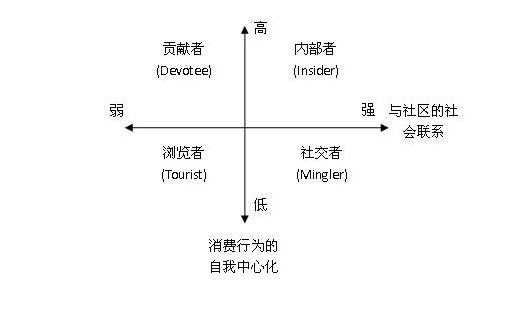
\includegraphics{users.jpg}
  \caption{虚拟社区的四种成员类型}
  \label{fig:user-type}
\end{figure}

杨堤雅进一步将虚拟社区成员分为了八种类别,并总结了每种类型成员的特征:
\begin{table}[htb]
  \centering \small
\caption{\small{虚拟社区成员角色及特征}} 
 \begin{tabular}{|c|c|c|c|c|}
    \hline
\backslashbox{特性}{角色} &参与程度&专业知识 &成员互动& 文章主要内容
\\\hline
成员领袖&高$\backslash$ 中&高&高&提供意见、分享经验\\\hline
意见呼应者&高$\backslash$ 中&中$\backslash$低&高&提供意见、分享经验
\\\hline
自我揭露者&中$\backslash$ 低&低&低&分享经验\\\hline
经验意见分享者&高$\backslash$ 中$\backslash$低$\backslash$路过&高
$\backslash$中&中&提供意见、分享经验\\\hline
查询者&低$\backslash$路过&中
$\backslash$低&中$\backslash$低&提问\\\hline
信息推广者&高$\backslash$ 中$\backslash$低$\backslash$路过&高
$\backslash$中&高$\backslash$ 中$\backslash$低&信息推广、建立关系
\\\hline
浏览者&---&低&低&无\\\hline
干扰者&低$\backslash$路过&低&低&其他\\\hline
  \end{tabular}
  
  \label{tab:characteristic}
\end{table}
\section{数据处理}
\label{sec:wikimedia-data}

维基基金会大约每隔3周就会对下属所有语言版本的维基百科的数据下载备份,
形成一个时间点的归档。备份的目的除了用于灾难回复外,更重要的是为所有有
志于参与维基百科学术研究的个人和团体提供数据支持。备份的内容除了所有条
目的内容外,还包括页面链接的列表以及图片元数据等内容。备份按照包涵内容
的不同分为3种类型:
\begin{itemize}
\item pages-articles备份。该类型的备份包含所有条目、模板和其它页面的当
  前版本,去除了条目的讨论页面和用户主页,适用于在其他地方再发布维基百
  科的内容。
\item pages-meta-current备份。提供所有页面的当前版本。
\item pages-meta-history备份。提供所有页面的所有历史版本,适合于学术研
  究。
\end{itemize}

本研究为了分析用户的协同行为并据此为其分类,因此需要研究用户的协同贡
献,比较所有历史版本同最后版本间的内容。显然,pages-meta-history备份包
含了研究所需要的全部数据。维基基金会提供了不同时段的pages-meta-history
备份,随着时间的推移,数据量显著增大。其中,最近的备份数据量在未压缩的情况下
达到了140Gb,数据的处理量非常大。为此,本研究选择了一个较小的数据集,
囊括了中文维基百科从创立值2008年8月的所有历史数据。数据集在未压缩情况
下大小为70Gb,存储格式为XML,其数据结构如下:

\begin{verbatim}
<page>
    <title>Wikipedia:Upload log</title>
    <id>1</id>
    <restrictions>sysop</restrictions>
    <revision>
      <id>288633</id>
      <timestamp>2002-12-11T09:10:02Z</timestamp>
      <contributor>
        <username>Formulax</username>
        <id>3</id>
      </contributor>
      <comment>uploaded &quot;Shanghai1.jpg&quot;: 上海夜景</comment>
      <text xml:space="preserve">Below is a list of the most recent file uploads.
       .........
    </revision>
</page>
\end{verbatim}

数据由一个个<page>组成,每个page是维基百科中的一个页面(如条目页面、讨
论页面、用户页面等)。每个page包括标题、id、以及所有的历史版本等信息。
其中page的标题由两部分组成,用“:”分割开:第一部分是该page所属的命名
空间;第二部分是该page实际的标题。这样,就可以通过标题判断出该page的实
际所属类型。
通常一个page中会包括多个版本。各个版本的内容记录在<revision>标签中,包
括版本的id、该版本修订的时间、作者的相关信息、每个版本的实际文字内容和
修订备注。利用这些信息,可以得到所有的用户协同行为的量化的属性值,为下
一步分析用户行为并分类做好数据准备。

\subsection{协同用户的选择}
\label{sec:user-exclude}

本文研究的对象是维基百科社区中的用户的协同行为。社区用户应该是具有正常
行为,努力为社区发展贡献力量的用户。但是,由于维基百科社区的开放性,各
类非正常的用户不断地涌现,不仅危害了社区的正常发展,也为相应的学术研究
带来了困难。维基百科社区中不正常的用户主要包括以下几种:
\begin{enumerate}
\item 被封禁的用户。这里用户通常是在社区中有不恰当的行为,例如攻击他人、
  广告宣传以及恶意地破坏等。封禁的目的只有一个,就是防止维基百科遭到持
  续或严重破坏。维基百科社区小心地对待各种不正常行为,谨慎使用封禁的权
  利。被封禁的用户绝大部分都出现过持续的非理性行为。因此本文认为被封禁
  的用户及其行为不应该被纳入到研究中来。
\item 傀儡用户。维基百科社区规定每位用户只能拥有一个帐号,防止用户使用
  傀儡来伪造对某件事的支持度,误导他人,挑起争端,协助破坏,或回避封禁。
  除非有及特殊的原因,傀儡帐号不用来参与同社区的知识协同活动,而是进行
  伪冒、滋扰等任何违反维基百科方针的行为。傀儡也不会纳入到本文的研究范
  围。
\item 用户名不规范的用户。用户名是每一个社区用户注册后的唯一标识。维基
  百科不允许使用带有误导性、宣传性、侮辱性或破坏性的用户名;也不允许用
  户名与现实世界中各组织或团体相关,或令人混淆于具体的人或组织。一旦发现具
  有以上特征的用户名,用户可以报告至“维基百科:需要管理员注意的用户名”页
  面并附上相关的解释,管理员可于审核以后把之封禁。上报不规范的用户
  名不意味着马上就会封禁,也就是说不会立刻出现在封禁列表中,但是历史记
  录表明绝大部分上报的用户名都受到了封禁。因此,本文排除了所有用户名不
  规范的用户。
\item 机器人用户。机器人是实际用户创建的为了完成特定目的,按照一定规则
  以自动化方式运行的账户。机器人对内容的操作极其有限,大部分机器人只能
  用于维护跨语言链接和修复重定向。除非有社群的批准,否则机器人不能用于
  拼写检查和纠正错字,以及处理繁简转换问题,尤其是对条目内容的检查。机
  器人本身并不创建任何内容,也不反应所属用户的协同行为和协同动机。本文
  的研究将机器人用户排除在外。
\item 匿名用户。关于匿名用户在维基百科社区中的作用一直是有争议的研究问
  题。就社区本身来说,尽管并不限制匿名用户的编辑,但是社区仍然鼓励用户
  注册一个账户,而非匿名编辑。维基百科认为匿名编辑的质量在本质是是存疑
  的,因此应该尽量避免。另一方面,匿名用户为识别用户带来了困难。匿名用
  户使用其IP地址作为其标识,这就意味着来自同一个IP地址的编辑可能实际上
  是由多个用户完成的,而单个用户也可能使用多个IP地址进行内容编辑。匿名
  用户本身并不是一个正常的用户状态,用户的行为也难以确认。同时,匿名用
  户本身的数量在所有用户中所占比例非常小,其贡献完全可以忽略。

\end{enumerate}

在所有的内容条目中,有一些条目也不适于纳入到研究范畴,需要从数据集中剔
除,主要包括:
\begin{enumerate}
\item 重定向页面。在维基百科中,经常会出现不同的用户针对相同的内容创建
  了不同的条目,例如“中华人民共和国”和“中国”两个条目本身的内容是一
  致的。为了避免这种情况,需要对两个条目进行合并,避免用户做重复工作,
  也使读者不会因此而产生困惑。重定向是一种特殊的页面,它提供一种运作机
  制,使得人们在输入该名称进入条目或者点击指向该名称的内部链接时,系统
  能够自动导航到重定向页面内部指定的另一相关页面中,从而实现相关页面可
  以以多个名称进行访问\footnote{http://zh.wikipedia.org/zh-cn/Help:重
    定向}。被重定向的页面将不再包含条目的实质内容,因此也就不存在用户
  的协同。
\item 消歧页和列表页。消歧义在维基百科中指消除由于不同条目拥有相同名称(一词多
  义)所引起的歧义。用户建立消歧页面,通过一些简单的注释内容消除混淆条目间的歧
  义,并引导读者链接到准确的具体的条目。列表页是为同一类别下的条目建立
  的索引式入口,如“亚洲国家列表”条目。列表页提供了该类下的所有条目的
  链接,方便导航读者。消歧页和列表页严格来说不算是合格的维基百科条目,
  而更像是方便读者的辅助性页面。另外,这两类页面的内容也常常由机器人完
  成。 
\end{enumerate}

\subsection{数据分析}
\label{sec:data-analysis}
通过对数据集的处理,提取内容条目,在去除了重定向页面、消歧页和列表页之后,共得到
205378个条目页面。所有的用户都围绕这些条目开展知识协同。社区中共有注册
用户55218名,占总用户数的$93\%$;另有数百名匿名用户和近百个机器人用户。这近六万名用户协
力完成了4592042次编辑,平均每个用户参与了77次编辑,每个条目得到了22次编辑。

利用上一章提出的计算用户协同贡献的方法,对数据进行处理。首先计算所有条
目的条目质量,计算的结果进行归一化。随后分别计算每个条目中参与用户各自
的贡献,最终可以得到每个用户在每次编辑后所做的贡献。将同一条目的编辑贡
献累加可以得到该用户为该条目所做的协同贡献,将用户所有编辑的贡献累加则
可以得到用户为整个社区所做的协同贡献。协同贡献计算完成后,本文进一步检
验了匿名用户在社区中的行为活动。匿名用户共参与了 96389个条目的知识协同活动,贡献了907763次编辑,分
别占总条目数的$46.9\%$以及总编辑次数的$19\%$。这个结果表明匿名用户似乎
是维基社区中的一股重要力量,不应该轻易舍弃。但是协同贡献的计算结果表
明,匿名用户的贡献度要远远低于注册用户的贡献度。注册用户平均每次编辑的
贡献达到了0.049,而匿名用户的平均贡献只有0.008,不及注册用户的六分之一。这
也验证了前文提到的匿名用户从从总体上来说
总的贡献来说,匿名用户的贡献只占总量的$3\%$。从匿名用户的数量和对社区的
贡献两方面因素考虑,本研究不考虑匿名用户的协同行为是合理的选择。

在将所有不适合
参与研究的用户从数据集中剔除,剩下的正常用户即为本文的研究对象,即维基
百科中参与或者试图参与知识协同的用户。这些用户在参与社区的协同编辑过程
中逐渐分化为不同的类别,每种类别均有各自不同的行为模式和特征。但是,同
其他类型的虚拟社区不同,已有的关于用户分类的研究并不完全适合本文的研究
对象。

首先,参与知识协同的用户并不存在传统意义上的潜水者(Lurker)和浏览者
(Browser)。潜水者和浏览者均是
社区的外围成员,他们加入社区的主要目的是为了消费社区的知识产品和信息产
品,几乎没有贡献内容的行为。Yong Du分析了这两类用户产生的原因,包括:1)
认为即使自己不贡献内容也不影响社区的运行;2)希望通过加入社区进一步了
解社区的相关情况;3)不愿意与他人分享自己的知识和经验\cite{4052703}。由于维基百科的
开放性,如果一个用户试图从维基百科获取有用信息,根本就不需要进行注册,
只是单纯浏览就可以了。注册用户都是在维基百科精神的感召下,对社区已经有
了一定的了解,愿意为之贡献自己的一份力量而进行注册的。即使一部分用户注
册完之后一次编辑行为也没有,这通常是由于没有找到合适的、可以参与的条
目,或者是不熟悉界面操作等因素造成的。因此,本文研究的用户群并不具备这
两类用户的特征。

其次,非协同用户已经被排除在外。大部分虚拟社区都不可避免地存在一些不受
欢迎的用户,如破坏者和广告发布者等。这些人不是以知识协同为目的参与到社
区中来的。本文在数据处理过程中已经将这些用户排除。从广义上讲,本文所研
究的协同用户都是实际的或者潜在的内容贡献者。

实际上,本文研究用户的分类实际上是研究虚拟社区中用户的一个子集,
即参与协同的用户的分类。因此传统的针对虚拟社区所有用户的分类并不适合,
需要寻找新的分类方法。这些协同用户参与维基百科社区具有相似的目的,但是仍可以根据其行
为特点划分出不同类别。

\subsection{分类维度}
\label{sec:dimension}
用户的协同行为可以从几个角度来考察,这些角度反映了用户协同的特点,从而
最终形成分类的依据。

用户对每个条目的平均贡献。用户对条目的平均贡献反映了一个用户的投入程度
及其价值。条目的贡献取决于用户自身的知识水平和其将知识转化为符合维基百
科标准的内容的能力。用
户所拥有的知识越多,越是积极参与该条目的编写,那么最终在条目中所作的贡
献就越大。
不同的用户的平均贡献相差非常大。图\ref{con-detri}显示了用户贡献不均衡
的分布情况。
\begin{figure}
  \label{con-detri}
  \centering
  \scalebox{0.7}{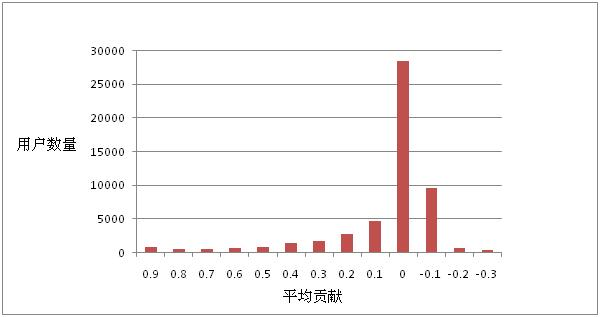
\includegraphics{con-distri.jpg}}
  \caption{\small{用户平均贡献分布}}
\end{figure}

图中显示了每个贡献度区间内的用户数量。可以看到贡献度的分布明显可以分为
几个部分。从0.9至0.5这个区间可以看出用户分布非常均匀,几乎每个区间段的
用户数量差别都不大。从0.5-0.1区间,用户数量开始稳步提升。在区间
[0.1,-0.1]之间用户数量暴涨,在这个区间的用户数达到了总用户数的$69\%$。
随后用户数量迅速减少。

不同区段的用户其特点也非常鲜明。对于平均贡献大于0.5的用户来说,这意味
着一个条目中有超过一半的内容是由该用户贡献的。称这名用户为该条目的主导
者毫不为过。这类用户除了亲自编写内容外,往往还会负责引领条目的编写方
向,规划内容的结构等,是组织条目编写的积极的带头人。对于平均贡献在0.1
至0.5这个区间的用户来说,他们尽管在知识协同中不占据主导力量,但是确实
整个协同过程中不可或缺的中坚力量。毕竟条目带头人的群体只占总用户数量的
$6.6\%$,面对数量如此众多的条目,仅靠这一小部分人是无法完成的。这类用
户是积极的追随者和稳定的实践者,按照条目编辑的预定目标,最大程度地贡献
自己的力量。最后一类用户是整个用户群体的低端用户,他们的平均贡献不超过
0.1。这意味着他们在条目编辑过程中所起的作用微不足道。甚至,平均贡献为
负值的用户占到了总用户数的$20.5\%$。从数值上看,很难说这个用户群体究竟
对维基百科社区起到了关键作用。但是,这个数量庞大的群体却是社区存在的坚
实基础。首先,高级用户产生于这个用户群体。任何的高级用户必然要经历一个
从初级用户到高级用户的过程,在这个过程中不断增加对社区的了解,不断提升
自己的技能和经验,最终才能带领其他用户共同建设一个繁荣的社区。只有拥有
数量庞大的初级用户群体,才会不断地产生更多的高级用户。其次,这些初级用
户所参与的工作大部分是维护性的工作,如修正条目中的错别字,改进内容的表
达方式,补充内容来源等工作。这些工作虽小,但是对于改进读者的阅读体验却有很大帮
助。因此,尽管这个用户群短期内对社区发展的影响很小,但是社区仍应将其视
为社区发展的重要资源。

另一个分类维度是用户参与编辑的条目数量。这个角度反映了用户的参与和活跃
程度。积极的用户往往不满足于参与有限的条目编辑中去,而是希望能尽可能地
为更多的条目贡献自己的力量。用户越是活跃,越
是积极参与,那么该用户所涉及到的条目也就越多。

同用户的平均贡献类似,用户参与的条目数量的分布也是极为不均衡。绝大部分
在其加入社区的整个生命周期内只参与了一、两个条目的协同。图\ref{fig:user-entry-1}显示了参与
条目数量在10以内的用户分布。
\begin{figure}[htb]
  \centering
 \scalebox{0.68}{ 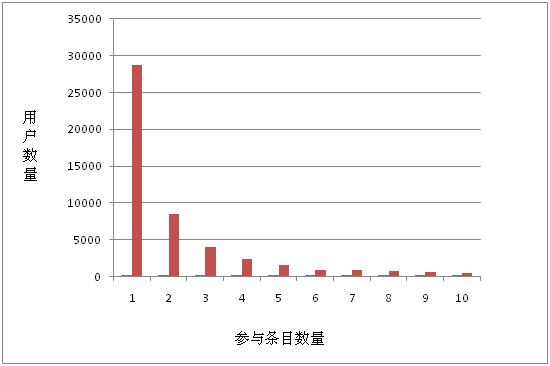
\includegraphics{user-entry-1.jpg}}
  \caption{\small{用户参与的条目数量}}
  \label{fig:user-entry-1}
\end{figure}

从图中可以看出,只参与了一个条目编写的用户数量达到了28749人,占总
用户数量的$52\%$。即有超过一半的用户处于这种极度不活跃的状态。而编辑条目数在5个以下的用户数共计45187人,占总用户数
量的$81.83\%$。这一部分用户可以视为社区中的不活跃人群,他们因为各种原
因没能找到发挥自己才能的条目,成为了沉默者。社区流失的成员大部分来自于
这个群体。从用户的分布数量看,编辑条目数量在1--5之间的用户数量从最大值
28749人急剧减少,随后,人数呈缓慢的下降趋势,由于数值太小,难以看出分
布随后的变化趋势。图\ref{fig:user-entry-2}进一步显示了较活跃的用户数量
的分布。
\begin{figure}[htb]
  \centering
 \scalebox{0.68}{ 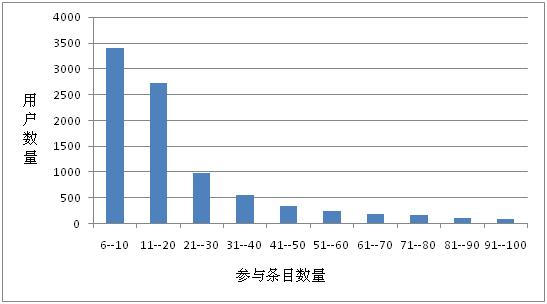
\includegraphics{user-entry-2.jpg}}
  \caption{\small{用户参与的条目数量2}}
  \label{fig:user-entry-2}
\end{figure}

图\ref{fig:user-entry-2}也表现出类似的用户分布。用户数量先是显著下降,
当到达51--60这个区间段后开始平缓下降。可以认为从这个区间段开始,用户表
现出了非常显著和活跃的协同行为。但一个用户参与条目的数量超过了50,表明
该用户已经完全熟悉并掌握了社区的基本规则,确立了自身的定位,并以一种非
常积极的态度参与到社区的协同活动中来。这一群体的用户是维基精神的积极践
行者。尽管他们可能不具有很多的专业知识,不能引领每一个条目的发展方向,
但是他们尽可能地发挥自身的优势,以巨大的热情为社区做出自己的贡献。在这
类用户中还存在着是一些“超人”用户:有10个用户参与的条目数量超过了
10000,其中参与条目最多的用户达到了23991个条目。正是这类活跃用户的努力
繁荣了整个社区。第三类用户是处于上述两
类用户之间的“中间用户”。这类用户逐渐从不活跃的状态向活跃状态转变,开始有
意识地寻找一些自己关心或是感兴趣的条目,试图从中发现可以贡献自身知识的
机会。另一方面,这一类用户由于时间、精力等方面的因素,没能象活跃用户那
样全情投入。尽管如此,由于人数上的优势(约为活跃用户的4倍),这类用户
仍然是社区繁荣的可靠力量。

通过以上分析的两个分类维度以及每个分类维度下的分类原则,最终可以得到适
用于分析用户协同行为及其特征的分类法。所有的用户按照该分类法都会分到一
个恰当的类别中去,分类的结果如表\ref{tab:category}所示:
\begin{table}[htb]
  \centering
 \small
 \caption{\small{用户分类结果}}
  \begin{tabular}{|c|c|c|c|c|}
\hline
    分类&条目平均贡献&参与条目数量&人数&百分比\\\hline
    分类1&高&高&61&$0.11\%$\\\hline
    分类2&高&中&224&$0.41\%$\\\hline
    分类3&高&低&3182&$5.76\%$\\\hline
    分类4&中&高&1027&$1.86\%$\\\hline
    分类5&中&中&2835&$5.13\%$\\\hline
    分类6&中&低&6866&$12.43\%$\\\hline
    分类7&低&高&1044&$1.89\%$\\\hline
    分类8&低&中&4839&$8.76\%$\\\hline
    分类9&低&低&35139&$63.64\%$\\\hline
  \end{tabular}
 
  \label{tab:category}
\end{table}

初始的分类结果形成了9个分类,并且不同分类间用户数量相差非常大。由于本
研究的目的是考察不同类型的用户参与知识协同的动机因素,考虑到形成的分类过多并且有些分类之间的界限并不明显,未能突出该类别的明
显特点,因此合并一些分类。合并的依据是,对于人数较少的分类合并到相似的
分类中;对于区分度不够明显的分类合并为一类。合并的结果为:分类2和分类3合并;分类4、分
类5及分类6合并;分类7和分类8合并。最终将维基百科的协同用户划分为5个类
别。
\begin{enumerate}
\item 领导者。这类用户的特点是广泛深入地参与到社区的协同活动中去。不但
  参与了大量条目的编辑工作,而且对于每个条目都积极投入,是协同编辑主要
  的领导者和最重要的贡献者。这类用户所占的比例极小,但是却起到了引领社
  区前进和发展的作用。领导者是社区最重要的用户群体。
\item 领域专家。这类用户的特点是对某些领域的知识精通。对于该领域下的条
  目具有独立撰写、或者领导其他用户共同完成编写条目的能力。对于每个参与
  的条目,他们都能深入地参与并贡献高质量的内容。同领导者群体
  不同,领域专家参与社区活动的热情要小得多,只求做好自己擅长的工作即可。
  因此他们实际参与的条目数量都比较小。
\item 内容贡献者。这类用户是协同活动的积极参与者。尽管他们限于自身的知识水
  平还不足以起到领导知识协同的作用,但是他们是专家和领导者的追随者。他
  们的工作对于补充、丰富条目的内容起到了重要的作用。对于前两类用户所忽
  视或者涉及不到的内容,都是由这类用户完成的。尽管由于时间和精力的原因
  他们参与的广泛程度不同,但是参与的动机基本是一致的。
\item 内容维护者。内容维护者的主要作用在于修补条目内容的疏漏,及时更新
  过时、无效的信息。对于每个条目,内容维护者参与的程度都不高,但是其参
  与的范围却很广泛。内容维护者自身并不具有太多的专业知识,但是他们通过
  维护内容的方式弥补了自身的不足,为改进条目质量和促进社区发展贡献力量。
\item 边缘用户。边缘用户是所有用户类别中数量最为庞大的群体。他们很少参
  与到协同活动中,即使偶尔参与协同也往往会由于经验不足而贡献低质量的内
  容,很快被回退或被其他用户修改。从主观上讲,边缘用户愿意参与到社区活
  动中,这是他们区别于破坏者和潜水者的显著特征。但是他们的意愿收到了某
  种客观条件的制约,一旦条件成熟,将促进边缘用户向更高级的用户转变。
\end{enumerate}

不同类型的用户间的关系如图\ref{fig:user-cat}所示。
\begin{figure}[htb]
  \centering
  \scalebox{0.51}{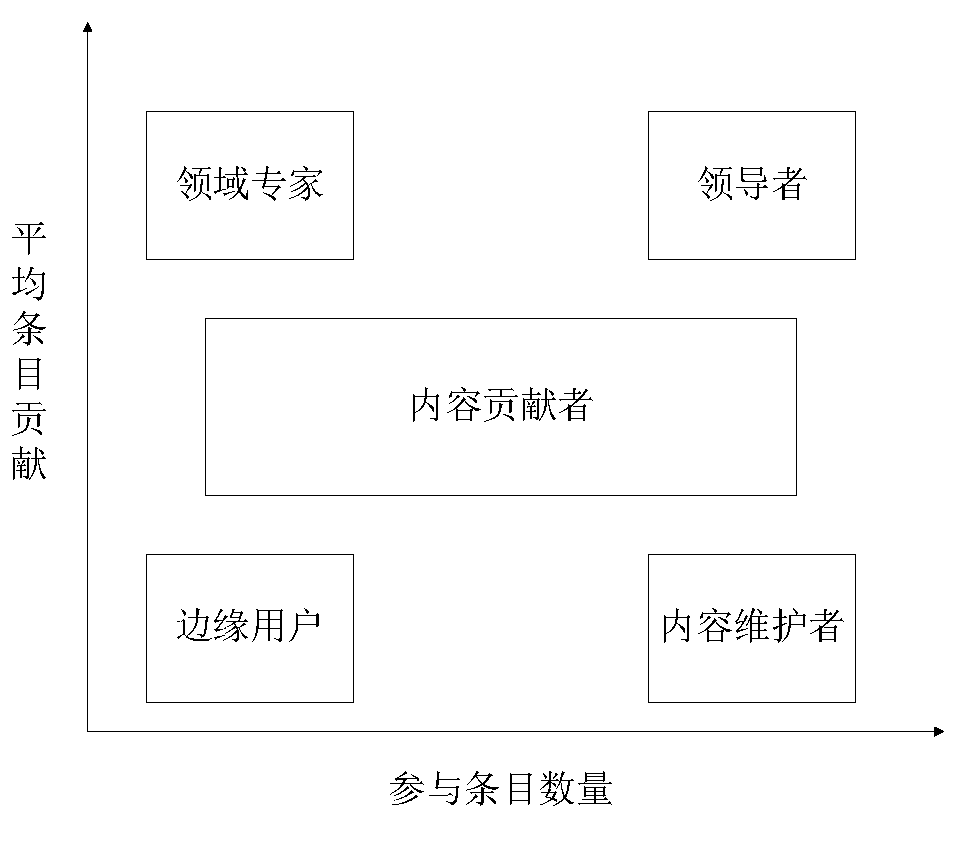
\includegraphics{user-cat.pdf}}
  \caption{\small{不同类型的用户间的关系}}
  \label{fig:user-cat}
\end{figure}
\section{用户协同的社会网络分析}
\label{sec:social-analysis}


至此,维基百科社区中的用户依据其贡献度和参与程度两个维度共分为5个类别。
同一类型用户之间的协同以及不同类型之间的用户协同构成了社区中的所有协同
活动。用户在协同中形成了用户间的复杂网络。运用社会网络分析手段,可以更
为清晰地理解维基百科社区中用户的协同
模式。

对于复杂网络的度量,往往使用图论来研究网络属性。由用户形成的复杂网络中,用户是网络中的节点,这些节点通过某种关系而连接
起来,形成了网络中的边。如果两个用户共同参与编辑了一个条目,则认为二者
进行了知识协同,形成了网络中的关联关系。

度(Degree)是复杂网络中最重要的度量之一。对于节点$i$,定义度$k_i$为与
该节点连接的其他节点的数目。在有向网络中还要进一步定义初度和入度。由于
协同关系是双相关联,即如果用户$A$与用户$B$协同一定意味着用户$B$与用户
$A$协同,因此用户网络实际上相当于无向图。在分析节点的度是主要考虑的指
标有三个:节点的平均度$\tilde{ k}=\frac{1}{N}\sum_i k_i$;节点的最大度
$k_{max}=max \  k_i$以及节点的度分布$P(k_i)$,它是节点度的概率分布函
数,表示节点$i$有$k$条边的概率。

集聚系数是衡量一个网络的集团化程度的重要的特征参数。在社会化网络中,如
果两个人同为一
个人的朋友,往往这两个人也是朋友。聚集系数就是为了表示网络中朋友圈的凝
聚成度,描述这种集团化现象的属性。一个节点$i$的聚集系数可以定义为于该
节点邻接的节点之间实际的连接数量同可能的最大连接数量的
比,即:$C_i=\frac{2E_i}{k_i(k_i-1)}$。其中$frac{k_i(k_i-1)}{2}$表示于
节点$i$邻接的节点间最大可能邻接数,而$E_i$是邻接节点间的实际连接数。这
样,通过聚集系数,可以反映不同群体间用户关联的紧密程度,从而分析其协同
模式。

领导者是所有类别中人数最少的,但是却是最为投入的群体。领导者共参与了37939
个条目的编写,平均每个人参与了622个条目。该类用户另外一个特点是:用户
参与的条目贡
献均值很高,但是贡献的方差却很大。在参与的所有条目中有$41.7\%$的条目贡献度
超过了0.8,几乎达到了单个领导者独立编写的程度;与之相对的有$39.2\%$的
条目领导者用户的贡献度
不足0.1。这个结果意味着领导者用户实际上存在着两种特征,除了自身用具有
的特征外还同时具有维护者的特征。通过进一步的分析发现,领导者用户所做的
维护工作同维护者所做的维护工作略有不同。领导者用户不是以消除文字错误、
更新信息等为目的的,而是为纠正其他用户错误的或不适当的行为为目的。由于
维基百科对用户参与的要求较高,除了必须有一定的独立撰写能力、遵从维基百
科的编写规范,还必须熟悉编写系统和标记语言的用法。对于没有经验的用户来
说很容易犯各种类型的错误。领导者于是承担起教育用户的责任,希望用户能在
参与编辑的过程中不断提升自身的水平。尽管这类用户同时存在这两种特征,但
是在接下来对用户参与知识协同活动的动机的研究中,将主要考虑领导者的特
征,而不考虑其维护者的特征。

领导者用户的最大度为42,但是平均度却只有9.2,超过一半的用户度在6一下,
说明领导者用户间很少有合作编写条目的经历,这和之前分析的领导者用户的特
征是一致的。同时,领导者的聚类系数只有0.17,远远小于整个社区的聚类系数
0.53。这说明用户之间并没有形成紧密联系的群体,一个用户也没有太多的意愿
去参与由另一个领导者主导的条目。用户间彼此的协同更多地是
在偶然的情况下发生的。

领域专家拥有和领导者类似的平均条目贡献,但是其参与条目的数量要小的多。
领域专家共计3406人,只参与了7424个条目的编写,平均每个人不到2.2个条目。
同领导者不同,领域专家的条目贡献离散程度要小的多,说明该类用户的协
同模式非常稳定:每参与到一个条目中,就尽全力把工作做好;而对于其他条目
则完全不理睬。

领域专家用户的最大度为4,平均度只有0.04,用户间的关联非常稀疏。网络的
聚集系数更是趋紧于0。这类用户比领导者用户还要独立,用户间的协同几乎不
发生。另外,领导者和领域专家两类用户之间也鲜有协同发生。
领域专家和领导者两类用户都属于能够主导条目编写的用户,
同时有领导者和领域
专家参与编写的条目共计403个,只占领域专家参于条目总数的$5.4\%$,对于领
导者来说更是微不足道。如果把两类用户合成一类共同考察的话,在新形成的用
户网络中,节点的最大度也只有103,而平均度也只达到了0.43,仍然是非常稀
疏的连接。网络的聚集系数值为0.03,显示用户之间几乎没有任何凝聚效应。

但是,这两类用户彼此之间很少发生协同行为并不意味着这两类用户真的是特立独行
的。事实上,
在有领域专家和领导者参与的条目中,参与协同的用户数量平均为127人/条目,
远远高于社区的均值46人/条目。尽管这两类用户掌控了条目的编辑工作,但是
似乎“独裁”并未影响用户的参与程度,反倒是
由于这两类用户的积极投入,给其他用户带来了更多的参与机会去丰富内容和提
升质量。

内容贡献者是所有用户中参与范围最广的群体,共参与了184746个条目的编写,
几乎占整个维基百科条目数量的$90\%$。平均每个用户参与编写17.2个条目。巨
大的参与数量意味着该类用户同其他几类用户都具有较强的联系。其中,内容贡
献者于领导者协作参与了24954个条目,占领导者参与总量的$65.77\%$;与领域
专家协作参与了5552个条目,占领域专家参与总量的$74.79\%$。说明内容贡
献者积极地参与了这两类用户领导的条目的编写工作。另外也应该注意到,尽管这两类用户都是维基百科社区的优质用户、
但是其参与的条目总数只占社区中条目总数的$21.9\%$。社区的精英并不能完成
所有的工作,还必须要依靠那些热心的普通用户配合。每个人的精力都是有限的。
对于维基百科这样完全依靠参与者在业余时间自愿投入的社区来说,明星用户永
远是少数,群体的力量才是真正可以依靠的力量。内容贡献者本身就承担了大量
的内容编写工作,是整个社区中力量最大的群体。

同领导者和领域专家不同,内容贡献者群体内部的协同非常频繁和活跃。网络节
点的最大度为7109,平均度为195,均远远高于其他两个类别。网络的聚集系数为
0.65,体现出了非常明显的聚集特征,意味着这一类用户的协同效应非常显著。
尽管他们每个人的能力都是有限的,但是他们依靠集体的
力量,相互合作,最终为社区做出自己的贡献。

维护者也是一个广泛参与知识协同的群体。该类用户共参与了143863个条目的编
写,约占条目总量的$70\%$。平均每个用户参与编辑24.5个条目。维护者与内容
贡献者的具有类似的网络特征。同上述几类用户的联系也非常紧密。其中,维护
者于领导者共同参与了21192个条目,占领导者参与总量的$55.86\%$;与领域专
家共同参与了5410个条目,占领域专家参与总量的$72.87\%$;与内容贡献者共
同参与了132539个条目,占维护者参与总量的$92.13\%$。可以看到,维护者于
社区中的主要成员关系都非常密切,尤其是和内容贡献者。

维护者群体内部的知识协同是所有类型用户中最为频繁和活跃的。其网络节点的
最大度数为5104,虽然不及内容贡献者的最大度,但是该类用户的数量只有内容
贡献者的一半,所以其平均度达到了320,为所有类别中最高。网络的聚集系数
为0.63,其聚集特征更为明显,成员之间的关系也更为密切。

边缘用户是人数最多的一类用户,但是却只参与了27732个条目的编写,平均没
人参与的条目为0.97个,是所有类型用户中最少的。边缘用户与其他类别的用户
协同则呈现明显的两极分化的特征。其于领导者共同参与了4299个条目,占边缘
用户参与总量的$15.49\%$;与领域专
家共同参与了1270个条目,占领域专家参与总量的$17.11\%$。而与之相对的,与内容贡献者共
同参与了27254个条目,占边缘用户参与总量的$98.28\%$,与维护用户共同参与
了26134个条目,占边缘用户参与总量的$94.24\%$。边缘用户几乎所有的协同都
是和内容贡献者和维护者之间发生的,而与领导者和领域专家间的协同则非常少。
这一方面是由于领导者和领域专家所参与条目的数量比较少,同时也是由于这两
类用户领导的条目质量普遍较高,并没有给边缘用户太多的参与机会。而内容贡
献者和维护者受自身条件的限制,给边缘用户留下了参与协同的空间。

边缘用户之间基本上没有什么直接联系,只有少数人具有较高的度。最大度为
151,但是有近$1/3$的用户度为0,也就是没有和任何其他边缘用户间发生过协
同,而网络平均度为9,表明连接是非常稀疏的。边缘用户的聚类系数为0.09,
证明用户之间非常独立,没有聚集特征。

通过社会网络分析,本文分析了维基百科社区中5类用户的协同行为和其特征。
可以明显地看出社区中主要存在两种形式的协同:一种是以领导者或者领域专家
为主导,内容贡献者和维护者参与辅助性工作最终完成条目的编写;另一种是参
与编写的条目中没有真正的主导者,而是由多个内容贡献者和维护者通力合作,
利用集体的力量共同完成的。这个结果同时也回答了人们一直以来对维基百科如
何取得成功而产生的疑问:究竟是“少数人的力量”还是“多数人的智慧”。一
部分学者认为如此数量巨大的内容不可能仅仅由少数人来完成,必然是很多人齐
心协力的结果;而维基百科的创始人Jimmy Wales则以英文维基百科为例,列举
了用户参与的数据:“有$50\%$的编辑是由不到$0.7\%$的用户完成的,最活跃
的$2\%$的用户,约1400人,则贡献了总编辑数量的$73.4\%$。本文的研究结果
表明,两种协同模式的
存在使得维基百科既体现了“少数人的力量”,由体现了“多数人的智慧”。少数明
星用户是社区最积极的推动力量,并取得了非常耀眼的成就,但是这并不意味着
其他用户就处于陪衬的角色。不同类型的用户通过不同的协同模式为社区贡献力量,最终才造就了维基百科的成
功。

\section{本章小结}
\label{sec:conclusion}

本章利用上一章研究的用户贡献算法,对维基百科中的数据进行整理和分析,并
从用户贡献和用户参与程度两个维度对维基百科社区中的用户进行了分类。分类
经过调整和合并后共分为五类:领导者、领域专家、内容贡献者、内容维护者以
及边缘用户。随后分析了这五类用户的特征,并使用社会网络分析研究了不同用
户的协同模式分析结果表明,这五类用户各自都有独特的协同模式,因此其参与
协同的动机可能各不相同。在随后的章节中将分别讨论各个动机因素对每种用户
的影响,构建每类用户的动机模型。
%%% Local Variables: 
%%% mode: latex
%%% TeX-master: t
%%% End: 

%The more
people involved, the slower and stupider their union is

the greater overhead imposed by the costs for coordination and
bureaucracy;
%%% Local Variables: 
%%% mode: latex
%%% TeX-master: t
%%% End: 

 
\chapter{知识协同动机因素模型仿真与决策分析}
\label{cha:emulation}

在上一章中,本文提出了个体参与社区知识协同的动机因素模型,描述了动机因
素与协同行为的关系。为了进一步验证模型的有效性,以及利用模型分析社区中
知识协同行为的演化过程,为管理决策提供依据,需要对模型进行仿真实验。

\section{动机因素模型仿真}

\subsection{仿真的基本过程}
建立模型要素的因果回路是模型仿真的第一步。但是仅靠因果回路图是无法进行
仿真的。因果回路图的适用范围是表达系统要素间的关联和反馈过程,但是变量
的性质却未能因果回路图中并没有表现出来。因果回路图无法描述系统管理和控
制过程,因此被应用于早期建模过程中,重点反应最基本的模型结构,方便建模
者对模型主体的把握。

流量和存量是社会经济系统中的两种基本变量。存量反映了系统在某一时刻的状
态,而流量则揭示了存量的变化快慢情况,这在因果图中是无法体现出来的。存
量变化的速率是系统演化的重要决定因素之一。因此,区分存量和流量是对因果
关系更细致和深入的描述,反应系统中各要素的控制与反馈。在存量流量模型的
基础上,通过设定各个变量的初值,步长等参数,用方程来描述各因素间的函数关
系,最终得到系统仿真的模型。通过多次试运行和调整,以及对模型进行有效性
检验,使模型可以较准确地反映现实世
界的变动,研究者可以利用模型进行决策分析。模型仿真的基本过程如图\ref{fig:vensim}所示。
\begin{figure}[htb]
  \centering
  \scalebox{0.7}{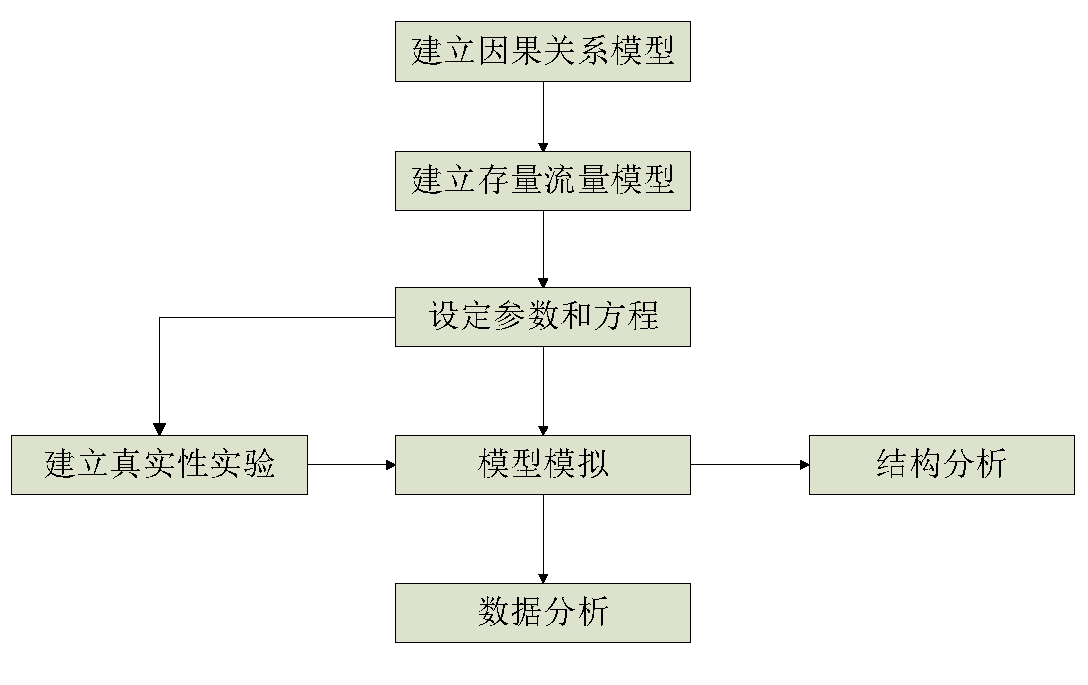
\includegraphics{vensim.pdf}}
  \caption{\small{\textbf{模型仿真过程}}}
  \label{fig:vensim}
\end{figure}
\subsection{动机因素存量流量图}

在因果图中,不论是动机因素,还是个体的行为都是系统的状态,是存量。为了
描述动机于行为间的关系而故意忽略了一些流量变量和外生变量。但是,这些被
忽略的变量对于整个系统起到了重要作用,没有这些变量系统就不可能正确地表
示现实系统的运行。

对于大部分动机因素,它们和个体的行为之间构成了一个正反馈回路和一个负反
馈回路,既动机的
增强会提升个体的行为水平,如果协同行为的得到了他人的正反馈,则会提升个体的动
机;反之如果协同行为得到了他人的负反馈,个体的动机会受到伤害。对于现实
系统来说,有几个重要的变量未能包含在因果图中。首先,个体的协同行为水平
不仅受到动机的影响,还受到其他因素,尤其是个体工作能力的限制。无论个体怎么
提升协同水平,都不可能超过个体的最大工作能力。这就是所谓“增长的极限”。
个体的最大工作能力是行为水平的抑制因素,使得行为水平不可能无限制地增长
下去。其次,动机作为系统中的存量,必然要受到流量的影响。动机的流
入是从协同活动中获得的正反馈转化的动机,动机的流出则是协同活动中获得的
负反馈使动机削弱的数量。流入水平和流出水平综合决定了动机存量的变化。第
三,不论是动机转化为行为还是行为的结果反馈影响动机都不是线性过程。这种
变换也存在遍及递减效应,动机的水平越高,每增加一单位动机所能引起的行为
水平的增加就越少。因此如果仅考虑行为与动机的互动关系的话,个体的动机应
该呈对数增长(或减弱),最后接近某个极大(小)值。最后,成就动机同其他
动机略有不同。成就动机促使个体参与某种活动从中获得成就感。成就感的提升
削弱成就需求。但是成就感有一种随时间自动削弱的属性,在没有任何外力介入
的情况下成就感将逐渐流失,从而提升了个体的成就需求,促使他们参与新的活
动重新获得成就感。流失速度的不同决定了不同人的行为模式,对于流失速度快
的人来说,他们从参与活动中所获得的成就感迅速减少,因此这些人表现为进取
精神非常强,不停地追逐新的目标来满足自己对成功的渴望。而流失速度慢的人则
会很长时间满足于自身取得的成就,表现为为止步不前,不愿接受新的挑战。

根据以上分析的结果,本文将把因果关系图转换为存量流量图,同时在模型中加
入新的变量,使模型更符合现实世界。因为转换的模型力图完整描述存量于流量
的关系,因此对因果关系进行了简化处理。变量间具体、详细的因果关系请参考
因果关系图。大部分的动机因素都有同样的特征:动机增加引起行为水平的提升;
如果行为得到正反馈则会促使动机也得到相应的提升,负反馈则会使动机减弱。。对于利他主义和感知到的意义两类动机由
于和行为之间是单向关系,行为的结果不会对这两个变量产生。影响。成就动机和认知失调两类动机有
各自的特点:成就动机根据满足感的变化而变化;认知失调的变化方向则和其他
因素相反,正反馈会减少认知失调水平,从而降低个体动机。在模型中引入了流量变量“每次协同行为增加的动机”表示
动机的流入,“他人对个体的协同行为减少的动机”表示动机的流出,以此表示
动机的动态性;引入变量“疲劳“和外生变量“个人工作的最大能力”构建行为
的负反馈闭环,反应行为水平受到抑制的特征。引入流量变量“满足感的流失”
反应满足感随时间减少的特点。转换的存量流量图如图
\ref{fig:refined-model}和图\ref{fig:refined-model2}所示。
\begin{figure}[!htb]
  \centering
  \scalebox{0.59}{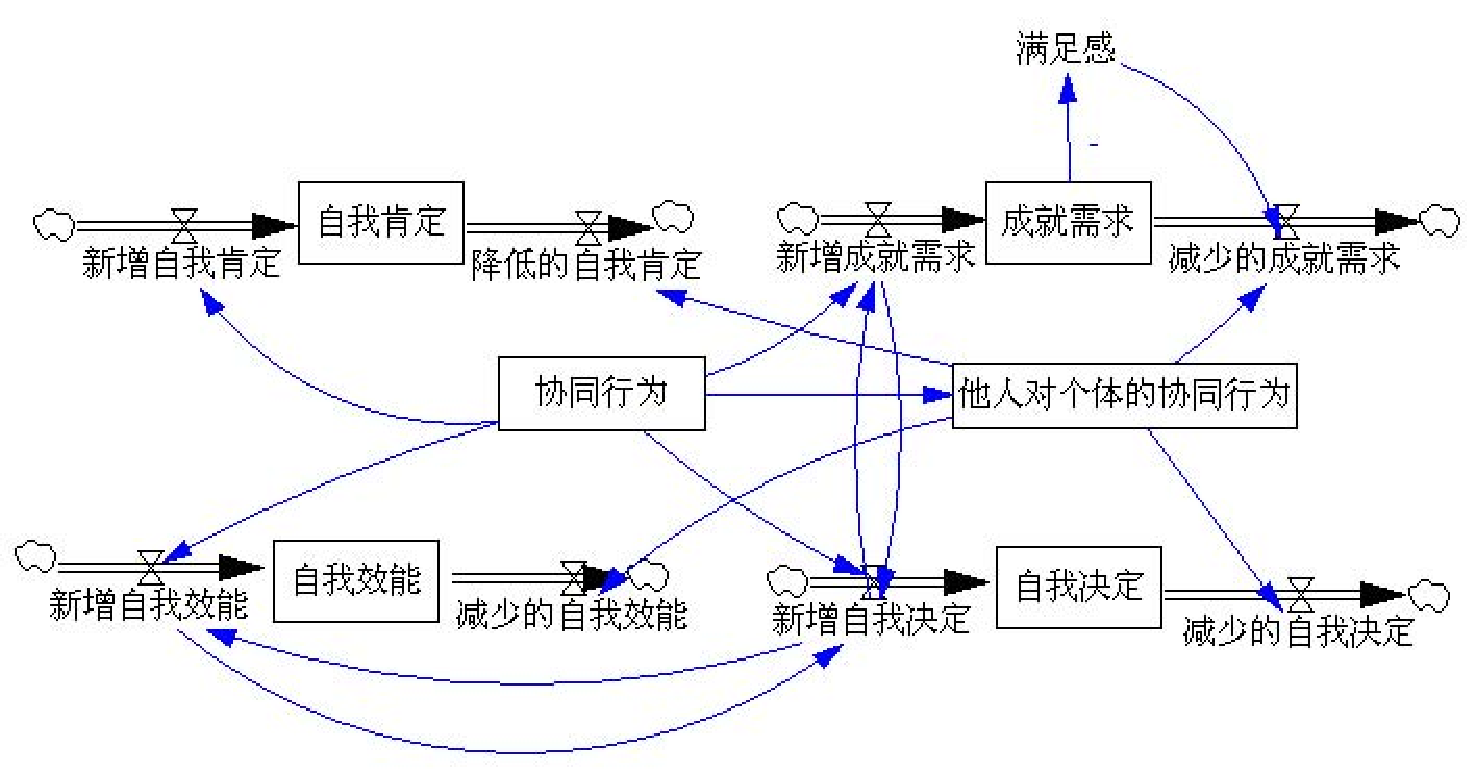
\includegraphics{io1.pdf}}
  \caption{\small{\textbf{知识协同个体动机因素的存量流量图}}}
  \label{fig:refined-model}
\end{figure}

\ref{fig:refined-model}所示。
\begin{figure}[!htb]
  \centering
  \scalebox{0.59}{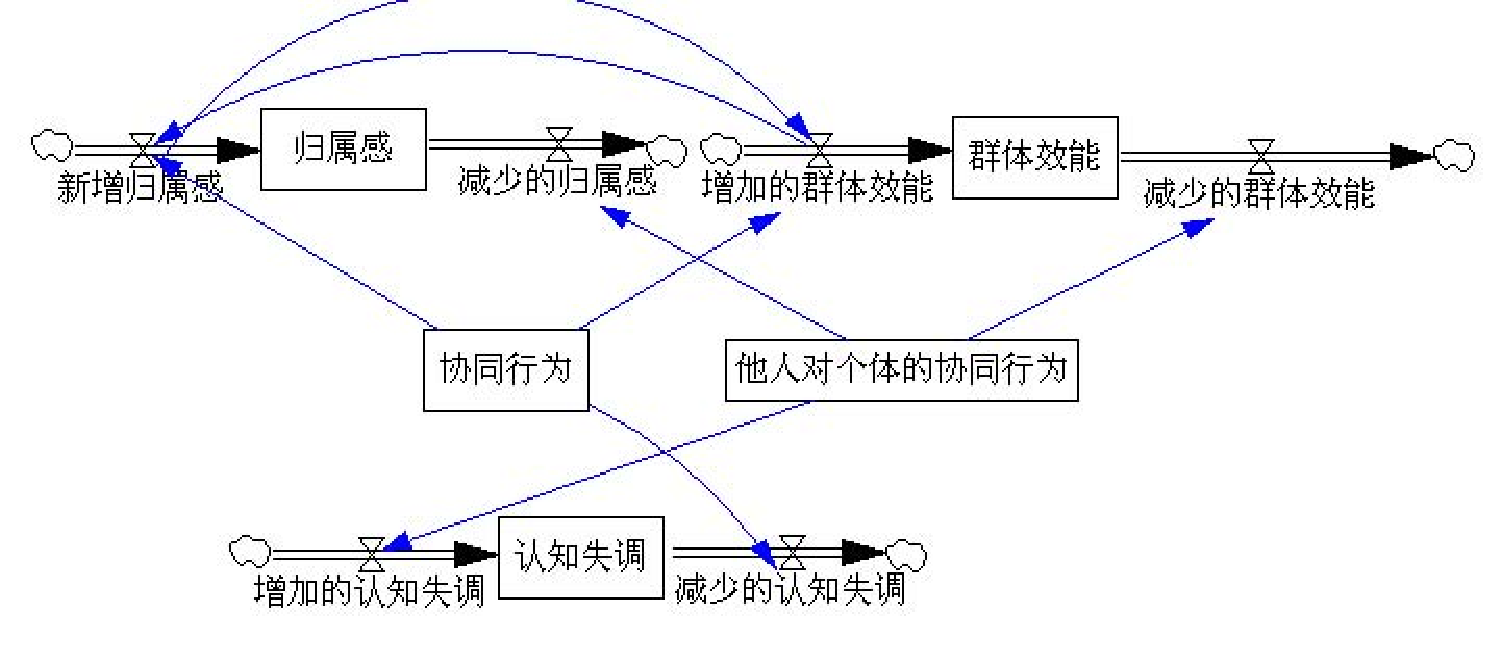
\includegraphics{io2.pdf}}
  \caption{\small{\textbf{知识协同人际间动机因素的存量流量图}}}
  \label{fig:refined-model2}
\end{figure}

\subsection{模型方程的设置}

每个变量都和其他变量形成一定的函数关系,这种关系使用方程来表示。下面列
举了了模型中所有涉及到的方程。其中称领导者和领域专家的模型为模型1,内
容贡献者、维护者和边缘用户的模型为模型2.
\begin{enumerate}
\item 模型1行为水平=转换水平$_1$$\times (\sum$成就动机+利他主
  义+感知到的意义+自我决定+自我效能+自我肯定)
\item 模型2行为水平=转换水平$_1$$\times (\sum$成就动机+利他主
  义+感知到的意义+自我决定+自我效能+自我肯定+认知失调+群体效能+归属感)
  
\item 成就需求=个体的最大成就需求-满足感$\times$转换系数+本期自我决定
  增量$\times$转换系数
\item 自我决定=上一期自我决定+正协同贡献$\times$转换系数+负协同贡献
  $\times$转换系数+本期自我效能增量 $\times$转换系数+本期归属感增量$\times$转换系数
\item  自我效能=上一期自我效能+正协同贡献$\times$转换系数+负协同贡献
  $\times$转换系数+本期自我决定增量 $\times$转换系数
\item 自我肯定=上一期自我肯定+正协同贡献$\times$转换系数+负协同贡献
  $\times$转换系数
\item 认知失调=他人的协同行为$\times$转换系数+他人对个体的协同行为
  $\times$转换系数-协同行为水平$\times$转换系数
\item 群体效能=上一期群体效能定+正协同贡献$\times$转换系数+负协同贡献
  $\times$转换系数+本期归属感增量$\times$转换系数
\item 归属感=上一期归属感+正协同贡献$\times$转换系数+负协同贡献
  $\times$转换系数+本期自我效能增量 $\times$转换系数+本期群体效能增量 $\times$转换系数



\end{enumerate}

\subsection{参数估计}
参数估计是建立系统动力学模型重要的过程。即使是参数值的微小变化,也可能会引起系统
行为产生较大幅度的波动,甚至改变整个系统行为的极
性。因此, 为保证模型模拟结果与真实系统的一致性, 应尽可能地准确估计模型
的参数。

模型的参数估计是模型的局部分别独立地进行,然后在总体模型进行模拟仿真时
在进行总的调试。系统动力学本身并不限制参数估计的方法,可以根据需要和具
体情况灵活地选用不同的参数估计方法。参数估计的完成标志着模型从定性向定
量的转化。

参数的估计方法可以分为以下几种。
目前SD 模型参数估计的技术大致可分为3 种[1, 2 ]: (1) 单个参数、表函数关系、间接计算等基于利用
模型变量集结程度以下的数据进行的估计; (2) 运用单方程进行估计; (3) 运用多方程进行估计等. 其中后
2 种都是基于与模型变量集结程度相当的数据进行的估计. 此外, 还可以运用统计技术进行估计.
但是, SD 模型基于结构而不是统计相关性的特征, 使得它所要求的许多参数(如国民经济系统中描述
人均国民收入对积累率影响程度的参数等) 往往缺乏可资利用的资料, 使建模工作者可以有效地运用前述
的种种方法对它们进行合理的估计. 还有一种情况, 由于SD 模型所处理的常是具有多重反馈的复杂系
统, 这使得处在因果链上相隔甚远的变量间的关系变得很不直观甚至反直观, 要估计描述它们对应关系的
参数也十分困难. 为了对这些难以估计的参数进行估计, 有时就得采用“仿真—分析—修正”这种类似于手
工式的“试凑法'' \cite{linwenhao2002}。

参数的估计工作分为两部分,一部分是估计变量的初值,另一部分是估计方程中
的参数。在动机因素于协同行为的模型中,大部分变量都是定性变量,本身就难
于量化。在缺乏资料的情况下,将定性变量数量化,本身就带有一定的盲目性和
随意性,因此手工调试是必不可少的环节。但是,通过使用一定的估计方法能大
大简化手工调试的工作量,减少调试的时间。

参数估计的结果如表\ref{tab:initail-value-level}和表\ref{tab:initail-value-transe}所示。
\begin{table}[!htbp]
  \centering
\small
  \caption{\small{\textbf{状态变量参数初始值}}}
% Table generated by Excel2LaTeX from sheet 'Sheet2'
\begin{tabular}{|c|c|c|c|c|c|}
\hline
\multicolumn{ 1}{|c|}{变量名称} &                                     \multicolumn{ 5}{|c|}{初始值} \\
\hline
\multicolumn{ 1}{|c|}{} &        领导者 &       领域专家 &      内容贡献者 &      内容维护者 &       边缘用户 \\
\hline
      利他主义 &      13      &        13    &        10    &   10         &      10      \\
\hline
    感知到的意义 &      10      &     10       &     10       &   10         &      10      \\
\hline
      自我决定 &      20      &     18       &      15      &          10  &    10        \\
\hline
      自我效能 &     25       &      15      &        15    &        8    &       5     \\
\hline
      自我肯定 &      25      &    15        &     10       &      10      &       10     \\
\hline
      成就需求 &     20       &     18       &      18      &      5      &        5    \\
\hline
      认知失调 &     $\slash$       &       $\slash$       &      10      &       15     &      9      \\
\hline
      群体效能 &     $\slash$         &          $\slash$    &    15        &      10      &       5     \\
\hline
       归属感 &       $\slash$       &     $\slash$         &      18      &        18    &        5    \\\hline
\end{tabular}  


  \label{tab:initail-value-level}
\end{table}

\begin{table}[!htb]
  \centering
\caption{\small{\textbf{转换系数初始值}}}
\small
% Table generated by Excel2LaTeX from sheet 'Sheet2'
\begin{tabular}{|c|c|c|c|c|c|}
\hline
\multicolumn{ 1}{|c|}{变量名称} &                                     \multicolumn{ 5}{|c|}{初始值} \\
\hline
\multicolumn{ 1}{|c|}{} &        领导者 &       领域专家 &      内容贡献者 &      内容维护者 &       边缘用户 \\
\hline
自我决定到协同水平的转换系数 &     0.003       &     0.003       &      0.002      &      0.001      &     0.001       \\
\hline
自我效能到协同水平的转换系数 &      0.005      &    0.005        &      0.006      &      0.008      &        0.008    \\
\hline
自我肯定到协同水平的转换系数 &      0.002     &       0.002    &      0.001      &     0.001       &       0.001     \\
\hline
成就需求到协同水平的转换系数 &     0.008       &     0.008       &     0.004       &         0.002   &       0.001     \\
\hline
认知失调到协同水平的转换系数 &      $\slash$       &    $\slash$         &    0.002        &         0.003   &      0.004      \\
\hline
群体效能到协同水平的转换系数 &          $\slash$    &       $\slash$       &   0.003         &    0.003        &        0.002    \\
\hline
归属感到协同水平的转换系数 &        $\slash$      &      $\slash$        &      0.003      &     0.003       &   0.003         \\
\hline
正协同贡献到自我决定的转换系数 &    0.0015        &    0.0014        &      0.0009      &        0.0006    &      0.0006      \\
\hline
正协同贡献到自我效能的转换系数 &    0.0022        &      0.0018      &       0.0013     &       0.0009     &  0.0009          \\
\hline
正协同贡献到自我肯定的转换系数 &     0.0014       &        0.0013    &     0.001       &        0.0006    &     0.0006       \\
\hline
正协同贡献到成就需求的转换系数 &       0.0008     &        0.0008    &      0.001      &       0.0008     &       0.0008     \\
\hline
正协同贡献到认知失调的转换系数 &     $\slash$        &     $\slash$        &    0.0007        &     0.0005       &       0.0006     \\
\hline
正协同贡献到群体效能的转换系数 &   $\slash$          &   $\slash$          &      0.0005      &     0.0005       &      0.0003      \\
\hline
正协同贡献到归属感的转换系数 &    $\slash$         &      $\slash$       &       0.0004     &      0.0005      &      0.0002      \\
\hline
负协同贡献到自我决定的转换系数 &     0.0001       &     0.0001       &    0.0005        &      0.0008      &     0.0009       \\
\hline
负协同贡献到自我效能的转换系数 &      0.0001      &     0.0001       &    0.0004        &      0.0009      &        0.001    \\
\hline
负协同贡献到自我肯定的转换系数 &     0.0001       &      0.0001
&0.0005&  0.0006            &  0.0006          \\
\hline
负协同贡献到成就需求的转换系数 &      0.0002      &       0.0002     &     0.0003       &       0.0003     &      0.0003      \\
\hline
负协同贡献到认知失调的转换系数 &       $\slash$      &    $\slash$         &    0.0002        &     0.0002       &     0.0001       \\
\hline
负协同贡献到群体效能的转换系数 &   $\slash$          &       $\slash$      &    0.0002        &       0.0002     &    0.0002        \\
\hline
负协同贡献到归属感的转换系数 &      $\slash$       &       $\slash$      &      0.0001      &        0.0003    &      0.0003      \\
\hline
\end{tabular}  

  
  \label{tab:initail-value-transe}
\end{table}

\section{模型检验}

当模型的所有参数都确定后,需要测试模型的有效性,检查模型是否能较准确地
模拟现实系统。模型的检验是一个不断证伪的过程。常见的检验方法包括结构评
价测试、参数估计测试、行为重现测试、灵敏度测试、系统改进测试等。检验往
往是通过同用户、专家的不断对话,深入理解系统行为,同时检查系统的因果关
系是否合理,方程量纲是否一致,对模型进行各种条件下的测试,并对比模型的
运行结果和实际数据。本文在参考大量文献的基础上,借鉴了其他学者的实证研
究成果,对模型进行历史检验,把模拟结果与历史数据进行
对照和比较, 以验证模型与客观系统的吻合程度, 从而判
定模型能否有效地反映客观系统,既观测模型是否能重现真实系统中的行为变化。
同时,对模型进行灵敏度检验,观测参数变化对于模型的影响。



模型是现实世界的简化和抽象,因此一个模型不可能精确地再现现实中的各种现
象。模型的主要目的在于反映趋势的变化。为了验证模型的正确性,本文将模型
仿真数据同真实数据进行对比。针对不同类型的用户,使用维基百科提供的数据分别计算了连续40个月的
月人均贡献度和仿真结果进行比对。

图\ref{fig:simu1}是领导者用户的仿真结果和真实数据图。从图中可以看出,领导者用户的月人
均贡献度呈现出比较明显的对数函数特征,而仿真的结果显示为系统行为呈现出
寻的模式,因此虽然模型同实际数据有误差,但是仍然较准确地再现了现实趋
势,可以使用模型模拟用户的知识协同行为。

\begin{figure}[!htb]
  \centering
 % \scalebox{0.65}{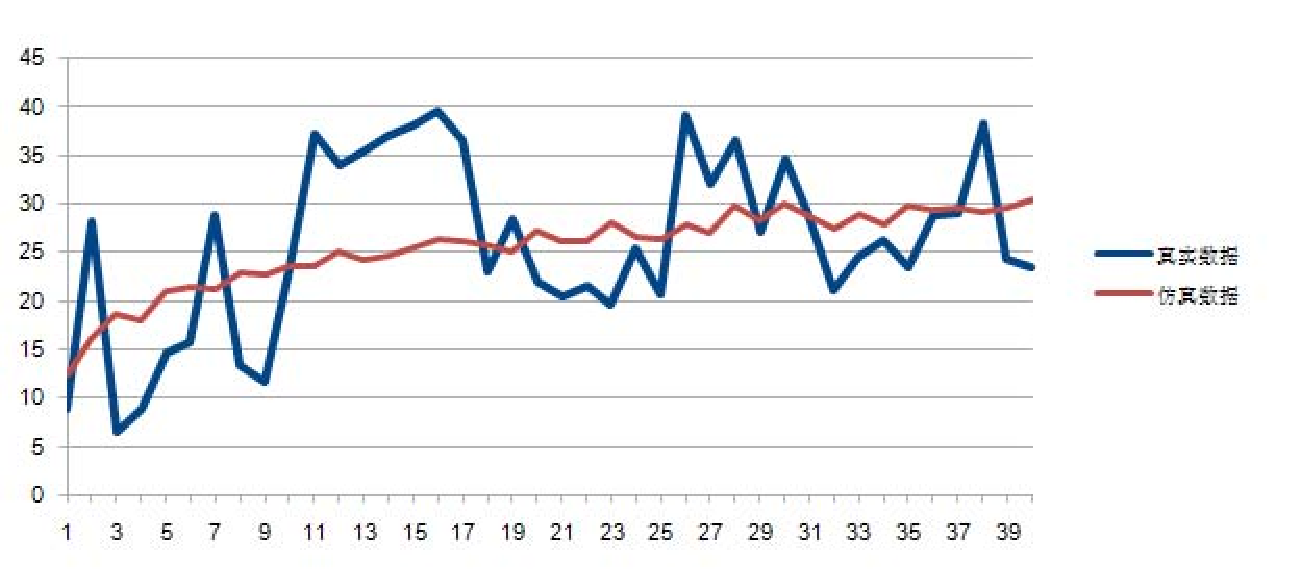
\includegraphics{simu-1.pdf}}
% GNUPLOT: LaTeX picture
\setlength{\unitlength}{0.240900pt}
\ifx\plotpoint\undefined\newsavebox{\plotpoint}\fi
\begin{picture}(1500,900)(0,0)
\sbox{\plotpoint}{\rule[-0.200pt]{0.400pt}{0.400pt}}%
\put(131.0,204.0){\rule[-0.200pt]{4.818pt}{0.400pt}}
\put(111,204){\makebox(0,0)[r]{5}}
\put(1419.0,204.0){\rule[-0.200pt]{4.818pt}{0.400pt}}
\put(131.0,277.0){\rule[-0.200pt]{4.818pt}{0.400pt}}
\put(111,277){\makebox(0,0)[r]{10}}
\put(1419.0,277.0){\rule[-0.200pt]{4.818pt}{0.400pt}}
\put(131.0,349.0){\rule[-0.200pt]{4.818pt}{0.400pt}}
\put(111,349){\makebox(0,0)[r]{15}}
\put(1419.0,349.0){\rule[-0.200pt]{4.818pt}{0.400pt}}
\put(131.0,422.0){\rule[-0.200pt]{4.818pt}{0.400pt}}
\put(111,422){\makebox(0,0)[r]{20}}
\put(1419.0,422.0){\rule[-0.200pt]{4.818pt}{0.400pt}}
\put(131.0,495.0){\rule[-0.200pt]{4.818pt}{0.400pt}}
\put(111,495){\makebox(0,0)[r]{25}}
\put(1419.0,495.0){\rule[-0.200pt]{4.818pt}{0.400pt}}
\put(131.0,568.0){\rule[-0.200pt]{4.818pt}{0.400pt}}
\put(111,568){\makebox(0,0)[r]{30}}
\put(1419.0,568.0){\rule[-0.200pt]{4.818pt}{0.400pt}}
\put(131.0,641.0){\rule[-0.200pt]{4.818pt}{0.400pt}}
\put(111,641){\makebox(0,0)[r]{35}}
\put(1419.0,641.0){\rule[-0.200pt]{4.818pt}{0.400pt}}
\put(131.0,713.0){\rule[-0.200pt]{4.818pt}{0.400pt}}
\put(111,713){\makebox(0,0)[r]{40}}
\put(1419.0,713.0){\rule[-0.200pt]{4.818pt}{0.400pt}}
\put(164.0,131.0){\rule[-0.200pt]{0.400pt}{4.818pt}}
\put(164,90){\makebox(0,0){ 1}}
\put(164.0,839.0){\rule[-0.200pt]{0.400pt}{4.818pt}}
\put(229.0,131.0){\rule[-0.200pt]{0.400pt}{4.818pt}}
\put(229,90){\makebox(0,0){ 3}}
\put(229.0,839.0){\rule[-0.200pt]{0.400pt}{4.818pt}}
\put(295.0,131.0){\rule[-0.200pt]{0.400pt}{4.818pt}}
\put(295,90){\makebox(0,0){ 5}}
\put(295.0,839.0){\rule[-0.200pt]{0.400pt}{4.818pt}}
\put(360.0,131.0){\rule[-0.200pt]{0.400pt}{4.818pt}}
\put(360,90){\makebox(0,0){ 7}}
\put(360.0,839.0){\rule[-0.200pt]{0.400pt}{4.818pt}}
\put(425.0,131.0){\rule[-0.200pt]{0.400pt}{4.818pt}}
\put(425,90){\makebox(0,0){ 9}}
\put(425.0,839.0){\rule[-0.200pt]{0.400pt}{4.818pt}}
\put(491.0,131.0){\rule[-0.200pt]{0.400pt}{4.818pt}}
\put(491,90){\makebox(0,0){ 11}}
\put(491.0,839.0){\rule[-0.200pt]{0.400pt}{4.818pt}}
\put(556.0,131.0){\rule[-0.200pt]{0.400pt}{4.818pt}}
\put(556,90){\makebox(0,0){ 13}}
\put(556.0,839.0){\rule[-0.200pt]{0.400pt}{4.818pt}}
\put(622.0,131.0){\rule[-0.200pt]{0.400pt}{4.818pt}}
\put(622,90){\makebox(0,0){ 15}}
\put(622.0,839.0){\rule[-0.200pt]{0.400pt}{4.818pt}}
\put(687.0,131.0){\rule[-0.200pt]{0.400pt}{4.818pt}}
\put(687,90){\makebox(0,0){ 17}}
\put(687.0,839.0){\rule[-0.200pt]{0.400pt}{4.818pt}}
\put(752.0,131.0){\rule[-0.200pt]{0.400pt}{4.818pt}}
\put(752,90){\makebox(0,0){ 19}}
\put(752.0,839.0){\rule[-0.200pt]{0.400pt}{4.818pt}}
\put(818.0,131.0){\rule[-0.200pt]{0.400pt}{4.818pt}}
\put(818,90){\makebox(0,0){ 21}}
\put(818.0,839.0){\rule[-0.200pt]{0.400pt}{4.818pt}}
\put(883.0,131.0){\rule[-0.200pt]{0.400pt}{4.818pt}}
\put(883,90){\makebox(0,0){ 23}}
\put(883.0,839.0){\rule[-0.200pt]{0.400pt}{4.818pt}}
\put(949.0,131.0){\rule[-0.200pt]{0.400pt}{4.818pt}}
\put(949,90){\makebox(0,0){ 25}}
\put(949.0,839.0){\rule[-0.200pt]{0.400pt}{4.818pt}}
\put(1014.0,131.0){\rule[-0.200pt]{0.400pt}{4.818pt}}
\put(1014,90){\makebox(0,0){ 27}}
\put(1014.0,839.0){\rule[-0.200pt]{0.400pt}{4.818pt}}
\put(1079.0,131.0){\rule[-0.200pt]{0.400pt}{4.818pt}}
\put(1079,90){\makebox(0,0){ 29}}
\put(1079.0,839.0){\rule[-0.200pt]{0.400pt}{4.818pt}}
\put(1145.0,131.0){\rule[-0.200pt]{0.400pt}{4.818pt}}
\put(1145,90){\makebox(0,0){ 31}}
\put(1145.0,839.0){\rule[-0.200pt]{0.400pt}{4.818pt}}
\put(1210.0,131.0){\rule[-0.200pt]{0.400pt}{4.818pt}}
\put(1210,90){\makebox(0,0){ 33}}
\put(1210.0,839.0){\rule[-0.200pt]{0.400pt}{4.818pt}}
\put(1276.0,131.0){\rule[-0.200pt]{0.400pt}{4.818pt}}
\put(1276,90){\makebox(0,0){ 35}}
\put(1276.0,839.0){\rule[-0.200pt]{0.400pt}{4.818pt}}
\put(1341.0,131.0){\rule[-0.200pt]{0.400pt}{4.818pt}}
\put(1341,90){\makebox(0,0){ 37}}
\put(1341.0,839.0){\rule[-0.200pt]{0.400pt}{4.818pt}}
\put(1406.0,131.0){\rule[-0.200pt]{0.400pt}{4.818pt}}
\put(1406,90){\makebox(0,0){ 39}}
\put(1406.0,839.0){\rule[-0.200pt]{0.400pt}{4.818pt}}
\put(131.0,131.0){\rule[-0.200pt]{0.400pt}{175.375pt}}
\put(131.0,131.0){\rule[-0.200pt]{315.097pt}{0.400pt}}
\put(1439.0,131.0){\rule[-0.200pt]{0.400pt}{175.375pt}}
\put(131.0,859.0){\rule[-0.200pt]{315.097pt}{0.400pt}}
\put(30,495){\makebox(0,0){\rotatebox{90}{用户贡献}}}
\put(785,29){\makebox(0,0){}}
\sbox{\plotpoint}{\rule[-0.400pt]{0.800pt}{0.800pt}}%
\sbox{\plotpoint}{\rule[-0.200pt]{0.400pt}{0.400pt}}%
\put(1279,819){\makebox(0,0)[r]{仿真数据}}
\sbox{\plotpoint}{\rule[-0.400pt]{0.800pt}{0.800pt}}%
\put(1299.0,819.0){\rule[-0.400pt]{24.090pt}{0.800pt}}
\put(164,309){\usebox{\plotpoint}}
\multiput(165.41,309.00)(0.503,0.785){57}{\rule{0.121pt}{1.450pt}}
\multiput(162.34,309.00)(32.000,46.990){2}{\rule{0.800pt}{0.725pt}}
\multiput(196.00,360.41)(0.568,0.504){51}{\rule{1.110pt}{0.121pt}}
\multiput(196.00,357.34)(30.695,29.000){2}{\rule{0.555pt}{0.800pt}}
\multiput(229.00,389.41)(0.793,0.505){35}{\rule{1.457pt}{0.122pt}}
\multiput(229.00,386.34)(29.976,21.000){2}{\rule{0.729pt}{0.800pt}}
\multiput(262.00,410.41)(1.055,0.507){25}{\rule{1.850pt}{0.122pt}}
\multiput(262.00,407.34)(29.160,16.000){2}{\rule{0.925pt}{0.800pt}}
\multiput(295.00,426.41)(1.278,0.509){19}{\rule{2.169pt}{0.123pt}}
\multiput(295.00,423.34)(27.498,13.000){2}{\rule{1.085pt}{0.800pt}}
\multiput(327.00,439.40)(1.586,0.512){15}{\rule{2.600pt}{0.123pt}}
\multiput(327.00,436.34)(27.604,11.000){2}{\rule{1.300pt}{0.800pt}}
\multiput(360.00,450.40)(1.768,0.514){13}{\rule{2.840pt}{0.124pt}}
\multiput(360.00,447.34)(27.105,10.000){2}{\rule{1.420pt}{0.800pt}}
\multiput(393.00,460.40)(1.936,0.516){11}{\rule{3.044pt}{0.124pt}}
\multiput(393.00,457.34)(25.681,9.000){2}{\rule{1.522pt}{0.800pt}}
\multiput(425.00,469.40)(2.752,0.526){7}{\rule{3.971pt}{0.127pt}}
\multiput(425.00,466.34)(24.757,7.000){2}{\rule{1.986pt}{0.800pt}}
\multiput(458.00,476.40)(2.752,0.526){7}{\rule{3.971pt}{0.127pt}}
\multiput(458.00,473.34)(24.757,7.000){2}{\rule{1.986pt}{0.800pt}}
\multiput(491.00,483.39)(3.365,0.536){5}{\rule{4.467pt}{0.129pt}}
\multiput(491.00,480.34)(22.729,6.000){2}{\rule{2.233pt}{0.800pt}}
\multiput(523.00,489.39)(3.476,0.536){5}{\rule{4.600pt}{0.129pt}}
\multiput(523.00,486.34)(23.452,6.000){2}{\rule{2.300pt}{0.800pt}}
\multiput(556.00,495.39)(3.476,0.536){5}{\rule{4.600pt}{0.129pt}}
\multiput(556.00,492.34)(23.452,6.000){2}{\rule{2.300pt}{0.800pt}}
\multiput(589.00,501.38)(5.126,0.560){3}{\rule{5.480pt}{0.135pt}}
\multiput(589.00,498.34)(21.626,5.000){2}{\rule{2.740pt}{0.800pt}}
\put(622,505.34){\rule{6.600pt}{0.800pt}}
\multiput(622.00,503.34)(18.301,4.000){2}{\rule{3.300pt}{0.800pt}}
\multiput(654.00,510.38)(5.126,0.560){3}{\rule{5.480pt}{0.135pt}}
\multiput(654.00,507.34)(21.626,5.000){2}{\rule{2.740pt}{0.800pt}}
\put(687,514.34){\rule{6.800pt}{0.800pt}}
\multiput(687.00,512.34)(18.886,4.000){2}{\rule{3.400pt}{0.800pt}}
\put(720,518.34){\rule{6.600pt}{0.800pt}}
\multiput(720.00,516.34)(18.301,4.000){2}{\rule{3.300pt}{0.800pt}}
\put(752,521.84){\rule{7.950pt}{0.800pt}}
\multiput(752.00,520.34)(16.500,3.000){2}{\rule{3.975pt}{0.800pt}}
\put(785,525.34){\rule{6.800pt}{0.800pt}}
\multiput(785.00,523.34)(18.886,4.000){2}{\rule{3.400pt}{0.800pt}}
\put(818,528.84){\rule{7.709pt}{0.800pt}}
\multiput(818.00,527.34)(16.000,3.000){2}{\rule{3.854pt}{0.800pt}}
\put(850,532.34){\rule{6.800pt}{0.800pt}}
\multiput(850.00,530.34)(18.886,4.000){2}{\rule{3.400pt}{0.800pt}}
\put(883,535.84){\rule{7.950pt}{0.800pt}}
\multiput(883.00,534.34)(16.500,3.000){2}{\rule{3.975pt}{0.800pt}}
\put(916,538.84){\rule{7.950pt}{0.800pt}}
\multiput(916.00,537.34)(16.500,3.000){2}{\rule{3.975pt}{0.800pt}}
\put(949,541.34){\rule{7.709pt}{0.800pt}}
\multiput(949.00,540.34)(16.000,2.000){2}{\rule{3.854pt}{0.800pt}}
\put(981,543.84){\rule{7.950pt}{0.800pt}}
\multiput(981.00,542.34)(16.500,3.000){2}{\rule{3.975pt}{0.800pt}}
\put(1014,546.84){\rule{7.950pt}{0.800pt}}
\multiput(1014.00,545.34)(16.500,3.000){2}{\rule{3.975pt}{0.800pt}}
\put(1047,549.34){\rule{7.709pt}{0.800pt}}
\multiput(1047.00,548.34)(16.000,2.000){2}{\rule{3.854pt}{0.800pt}}
\put(1079,551.84){\rule{7.950pt}{0.800pt}}
\multiput(1079.00,550.34)(16.500,3.000){2}{\rule{3.975pt}{0.800pt}}
\put(1112,554.34){\rule{7.950pt}{0.800pt}}
\multiput(1112.00,553.34)(16.500,2.000){2}{\rule{3.975pt}{0.800pt}}
\put(1145,556.84){\rule{7.709pt}{0.800pt}}
\multiput(1145.00,555.34)(16.000,3.000){2}{\rule{3.854pt}{0.800pt}}
\put(1177,559.34){\rule{7.950pt}{0.800pt}}
\multiput(1177.00,558.34)(16.500,2.000){2}{\rule{3.975pt}{0.800pt}}
\put(1210,561.34){\rule{7.950pt}{0.800pt}}
\multiput(1210.00,560.34)(16.500,2.000){2}{\rule{3.975pt}{0.800pt}}
\put(1243,563.34){\rule{7.950pt}{0.800pt}}
\multiput(1243.00,562.34)(16.500,2.000){2}{\rule{3.975pt}{0.800pt}}
\put(1276,565.34){\rule{7.709pt}{0.800pt}}
\multiput(1276.00,564.34)(16.000,2.000){2}{\rule{3.854pt}{0.800pt}}
\put(1308,567.34){\rule{7.950pt}{0.800pt}}
\multiput(1308.00,566.34)(16.500,2.000){2}{\rule{3.975pt}{0.800pt}}
\put(1341,569.34){\rule{7.950pt}{0.800pt}}
\multiput(1341.00,568.34)(16.500,2.000){2}{\rule{3.975pt}{0.800pt}}
\put(1374,571.34){\rule{7.709pt}{0.800pt}}
\multiput(1374.00,570.34)(16.000,2.000){2}{\rule{3.854pt}{0.800pt}}
\put(1406,573.34){\rule{7.950pt}{0.800pt}}
\multiput(1406.00,572.34)(16.500,2.000){2}{\rule{3.975pt}{0.800pt}}
\sbox{\plotpoint}{\rule[-0.200pt]{0.400pt}{0.400pt}}%
\put(1279,769){\makebox(0,0)[r]{实际数据}}
\put(1299.0,778.0){\rule[-0.200pt]{24.090pt}{0.400pt}}
\put(164,260){\usebox{\plotpoint}}
\multiput(164.58,260.00)(0.497,4.449){61}{\rule{0.120pt}{3.625pt}}
\multiput(163.17,260.00)(32.000,274.476){2}{\rule{0.400pt}{1.813pt}}
\multiput(196.58,533.03)(0.497,-2.597){63}{\rule{0.120pt}{2.161pt}}
\multiput(195.17,537.52)(33.000,-165.516){2}{\rule{0.400pt}{1.080pt}}
\multiput(229.58,372.00)(0.497,0.514){63}{\rule{0.120pt}{0.512pt}}
\multiput(228.17,372.00)(33.000,32.937){2}{\rule{0.400pt}{0.256pt}}
\multiput(262.58,402.52)(0.497,-0.928){63}{\rule{0.120pt}{0.839pt}}
\multiput(261.17,404.26)(33.000,-59.258){2}{\rule{0.400pt}{0.420pt}}
\multiput(295.00,345.58)(1.009,0.494){29}{\rule{0.900pt}{0.119pt}}
\multiput(295.00,344.17)(30.132,16.000){2}{\rule{0.450pt}{0.400pt}}
\multiput(327.58,361.00)(0.497,2.919){63}{\rule{0.120pt}{2.415pt}}
\multiput(326.17,361.00)(33.000,185.987){2}{\rule{0.400pt}{1.208pt}}
\multiput(360.58,543.94)(0.497,-2.322){63}{\rule{0.120pt}{1.942pt}}
\multiput(359.17,547.97)(33.000,-147.968){2}{\rule{0.400pt}{0.971pt}}
\multiput(393.58,400.00)(0.497,0.736){61}{\rule{0.120pt}{0.688pt}}
\multiput(392.17,400.00)(32.000,45.573){2}{\rule{0.400pt}{0.344pt}}
\multiput(425.00,447.58)(0.661,0.497){47}{\rule{0.628pt}{0.120pt}}
\multiput(425.00,446.17)(31.697,25.000){2}{\rule{0.314pt}{0.400pt}}
\multiput(458.58,472.00)(0.497,0.820){63}{\rule{0.120pt}{0.755pt}}
\multiput(457.17,472.00)(33.000,52.434){2}{\rule{0.400pt}{0.377pt}}
\multiput(491.58,526.00)(0.497,1.542){61}{\rule{0.120pt}{1.325pt}}
\multiput(490.17,526.00)(32.000,95.250){2}{\rule{0.400pt}{0.663pt}}
\multiput(523.58,621.87)(0.497,-0.514){63}{\rule{0.120pt}{0.512pt}}
\multiput(522.17,622.94)(33.000,-32.937){2}{\rule{0.400pt}{0.256pt}}
\multiput(556.00,590.58)(0.752,0.496){41}{\rule{0.700pt}{0.120pt}}
\multiput(556.00,589.17)(31.547,22.000){2}{\rule{0.350pt}{0.400pt}}
\multiput(589.00,610.92)(0.549,-0.497){57}{\rule{0.540pt}{0.120pt}}
\multiput(589.00,611.17)(31.879,-30.000){2}{\rule{0.270pt}{0.400pt}}
\multiput(622.00,580.93)(2.841,-0.482){9}{\rule{2.233pt}{0.116pt}}
\multiput(622.00,581.17)(27.365,-6.000){2}{\rule{1.117pt}{0.400pt}}
\multiput(654.58,576.00)(0.497,0.652){63}{\rule{0.120pt}{0.621pt}}
\multiput(653.17,576.00)(33.000,41.711){2}{\rule{0.400pt}{0.311pt}}
\multiput(687.58,612.40)(0.497,-1.877){63}{\rule{0.120pt}{1.591pt}}
\multiput(686.17,615.70)(33.000,-119.698){2}{\rule{0.400pt}{0.795pt}}
\multiput(720.58,496.00)(0.497,0.752){61}{\rule{0.120pt}{0.700pt}}
\multiput(719.17,496.00)(32.000,46.547){2}{\rule{0.400pt}{0.350pt}}
\multiput(752.00,542.93)(2.476,-0.485){11}{\rule{1.986pt}{0.117pt}}
\multiput(752.00,543.17)(28.879,-7.000){2}{\rule{0.993pt}{0.400pt}}
\multiput(785.58,534.77)(0.497,-0.545){63}{\rule{0.120pt}{0.536pt}}
\multiput(784.17,535.89)(33.000,-34.887){2}{\rule{0.400pt}{0.268pt}}
\multiput(818.00,501.58)(1.009,0.494){29}{\rule{0.900pt}{0.119pt}}
\multiput(818.00,500.17)(30.132,16.000){2}{\rule{0.450pt}{0.400pt}}
\multiput(850.00,515.92)(0.589,-0.497){53}{\rule{0.571pt}{0.120pt}}
\multiput(850.00,516.17)(31.814,-28.000){2}{\rule{0.286pt}{0.400pt}}
\multiput(883.00,489.58)(1.290,0.493){23}{\rule{1.115pt}{0.119pt}}
\multiput(883.00,488.17)(30.685,13.000){2}{\rule{0.558pt}{0.400pt}}
\multiput(916.58,502.00)(0.497,0.912){63}{\rule{0.120pt}{0.827pt}}
\multiput(915.17,502.00)(33.000,58.283){2}{\rule{0.400pt}{0.414pt}}
\multiput(949.58,562.00)(0.497,1.036){61}{\rule{0.120pt}{0.925pt}}
\multiput(948.17,562.00)(32.000,64.080){2}{\rule{0.400pt}{0.463pt}}
\multiput(981.00,626.92)(0.549,-0.497){57}{\rule{0.540pt}{0.120pt}}
\multiput(981.00,627.17)(31.879,-30.000){2}{\rule{0.270pt}{0.400pt}}
\multiput(1014.00,596.93)(2.476,-0.485){11}{\rule{1.986pt}{0.117pt}}
\multiput(1014.00,597.17)(28.879,-7.000){2}{\rule{0.993pt}{0.400pt}}
\multiput(1047.58,587.21)(0.497,-1.020){61}{\rule{0.120pt}{0.913pt}}
\multiput(1046.17,589.11)(32.000,-63.106){2}{\rule{0.400pt}{0.456pt}}
\multiput(1079.58,526.00)(0.497,1.663){63}{\rule{0.120pt}{1.421pt}}
\multiput(1078.17,526.00)(33.000,106.050){2}{\rule{0.400pt}{0.711pt}}
\multiput(1112.58,630.41)(0.497,-1.265){63}{\rule{0.120pt}{1.106pt}}
\multiput(1111.17,632.70)(33.000,-80.704){2}{\rule{0.400pt}{0.553pt}}
\multiput(1145.58,552.00)(0.497,0.515){61}{\rule{0.120pt}{0.512pt}}
\multiput(1144.17,552.00)(32.000,31.936){2}{\rule{0.400pt}{0.256pt}}
\multiput(1177.58,585.00)(0.497,0.744){63}{\rule{0.120pt}{0.694pt}}
\multiput(1176.17,585.00)(33.000,47.560){2}{\rule{0.400pt}{0.347pt}}
\multiput(1210.58,627.45)(0.497,-1.862){63}{\rule{0.120pt}{1.579pt}}
\multiput(1209.17,630.72)(33.000,-118.723){2}{\rule{0.400pt}{0.789pt}}
\multiput(1243.58,512.00)(0.497,1.617){63}{\rule{0.120pt}{1.385pt}}
\multiput(1242.17,512.00)(33.000,103.126){2}{\rule{0.400pt}{0.692pt}}
\multiput(1276.58,614.06)(0.497,-1.068){61}{\rule{0.120pt}{0.950pt}}
\multiput(1275.17,616.03)(32.000,-66.028){2}{\rule{0.400pt}{0.475pt}}
\multiput(1308.00,550.59)(3.604,0.477){7}{\rule{2.740pt}{0.115pt}}
\multiput(1308.00,549.17)(27.313,5.000){2}{\rule{1.370pt}{0.400pt}}
\multiput(1341.58,555.00)(0.497,1.586){63}{\rule{0.120pt}{1.361pt}}
\multiput(1340.17,555.00)(33.000,101.176){2}{\rule{0.400pt}{0.680pt}}
\multiput(1374.00,657.92)(0.551,-0.497){55}{\rule{0.541pt}{0.120pt}}
\multiput(1374.00,658.17)(30.876,-29.000){2}{\rule{0.271pt}{0.400pt}}
\multiput(1406.00,628.92)(1.290,-0.493){23}{\rule{1.115pt}{0.119pt}}
\multiput(1406.00,629.17)(30.685,-13.000){2}{\rule{0.558pt}{0.400pt}}
\put(164,260){\makebox(0,0){$+$}}
\put(196,542){\makebox(0,0){$+$}}
\put(229,372){\makebox(0,0){$+$}}
\put(262,406){\makebox(0,0){$+$}}
\put(295,345){\makebox(0,0){$+$}}
\put(327,361){\makebox(0,0){$+$}}
\put(360,552){\makebox(0,0){$+$}}
\put(393,400){\makebox(0,0){$+$}}
\put(425,447){\makebox(0,0){$+$}}
\put(458,472){\makebox(0,0){$+$}}
\put(491,526){\makebox(0,0){$+$}}
\put(523,624){\makebox(0,0){$+$}}
\put(556,590){\makebox(0,0){$+$}}
\put(589,612){\makebox(0,0){$+$}}
\put(622,582){\makebox(0,0){$+$}}
\put(654,576){\makebox(0,0){$+$}}
\put(687,619){\makebox(0,0){$+$}}
\put(720,496){\makebox(0,0){$+$}}
\put(752,544){\makebox(0,0){$+$}}
\put(785,537){\makebox(0,0){$+$}}
\put(818,501){\makebox(0,0){$+$}}
\put(850,517){\makebox(0,0){$+$}}
\put(883,489){\makebox(0,0){$+$}}
\put(916,502){\makebox(0,0){$+$}}
\put(949,562){\makebox(0,0){$+$}}
\put(981,628){\makebox(0,0){$+$}}
\put(1014,598){\makebox(0,0){$+$}}
\put(1047,591){\makebox(0,0){$+$}}
\put(1079,526){\makebox(0,0){$+$}}
\put(1112,635){\makebox(0,0){$+$}}
\put(1145,552){\makebox(0,0){$+$}}
\put(1177,585){\makebox(0,0){$+$}}
\put(1210,634){\makebox(0,0){$+$}}
\put(1243,512){\makebox(0,0){$+$}}
\put(1276,618){\makebox(0,0){$+$}}
\put(1308,550){\makebox(0,0){$+$}}
\put(1341,555){\makebox(0,0){$+$}}
\put(1374,659){\makebox(0,0){$+$}}
\put(1406,630){\makebox(0,0){$+$}}
\put(1439,617){\makebox(0,0){$+$}}
\put(1349,778){\makebox(0,0){$+$}}
\put(131.0,131.0){\rule[-0.200pt]{0.400pt}{175.375pt}}
\put(131.0,131.0){\rule[-0.200pt]{315.097pt}{0.400pt}}
\put(1439.0,131.0){\rule[-0.200pt]{0.400pt}{175.375pt}}
\put(131.0,859.0){\rule[-0.200pt]{315.097pt}{0.400pt}}
\end{picture}
 
 \caption{\small{\textbf{领导者用户仿真结果}}}
  \label{fig:simu1}
\end{figure}

图\ref{fig:simu2}是领域专家用户的仿真结果和真实数据图。真实数据反映出该类用户的月人均
贡献度在初期显著下降后迅速进入一个平稳状态。仿真结果则表现为一个递减
的对数函数。两者的趋势是一致的。

\begin{figure}[!htb]
  \centering
%  \scalebox{0.65}{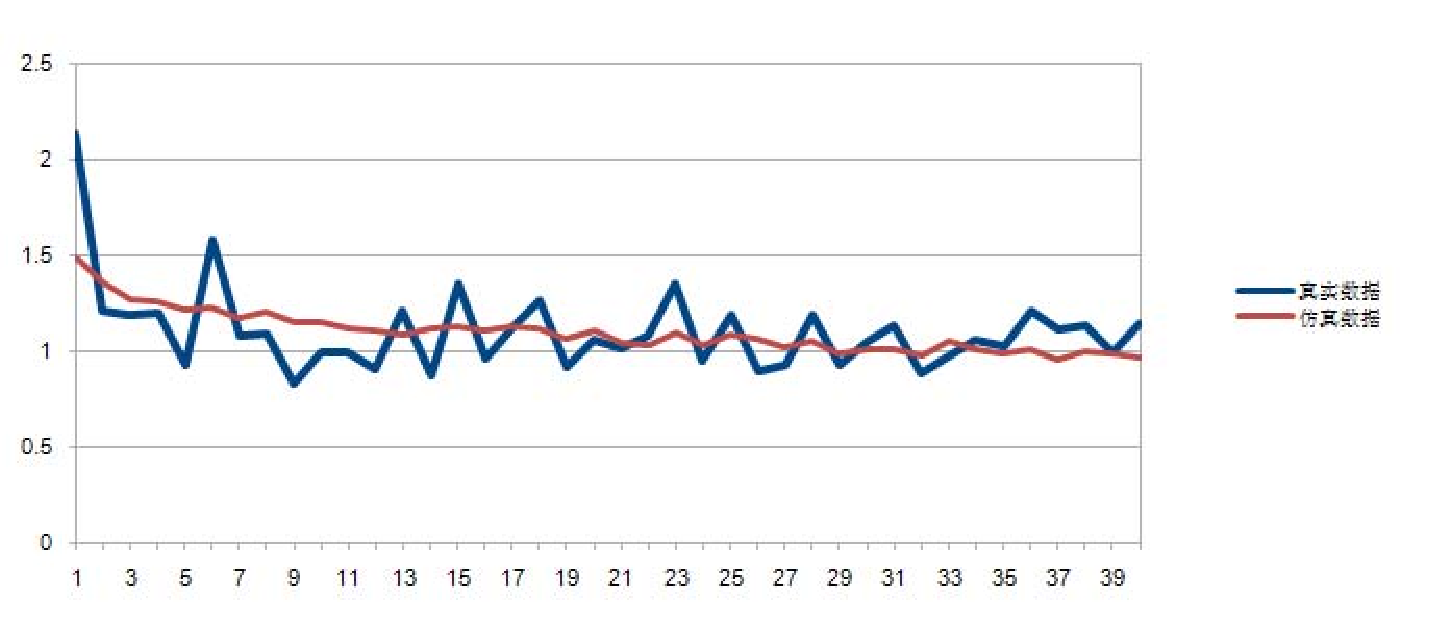
\includegraphics{simu-2.pdf}}
 % GNUPLOT: LaTeX picture
\setlength{\unitlength}{0.240900pt}
\ifx\plotpoint\undefined\newsavebox{\plotpoint}\fi
\begin{picture}(1500,900)(0,0)
\sbox{\plotpoint}{\rule[-0.200pt]{0.400pt}{0.400pt}}%
\put(131.0,82.0){\rule[-0.200pt]{4.818pt}{0.400pt}}
\put(111,82){\makebox(0,0)[r]{ 0}}
\put(1419.0,82.0){\rule[-0.200pt]{4.818pt}{0.400pt}}
\put(131.0,341.0){\rule[-0.200pt]{4.818pt}{0.400pt}}
\put(111,341){\makebox(0,0)[r]{ 1}}
\put(1419.0,341.0){\rule[-0.200pt]{4.818pt}{0.400pt}}
\put(131.0,600.0){\rule[-0.200pt]{4.818pt}{0.400pt}}
\put(111,600){\makebox(0,0)[r]{ 2}}
\put(1419.0,600.0){\rule[-0.200pt]{4.818pt}{0.400pt}}
\put(131.0,859.0){\rule[-0.200pt]{4.818pt}{0.400pt}}
\put(111,859){\makebox(0,0)[r]{ 3}}
\put(1419.0,859.0){\rule[-0.200pt]{4.818pt}{0.400pt}}
\put(131.0,82.0){\rule[-0.200pt]{0.400pt}{4.818pt}}
\put(131,41){\makebox(0,0){ 1}}
\put(131.0,839.0){\rule[-0.200pt]{0.400pt}{4.818pt}}
\put(198.0,82.0){\rule[-0.200pt]{0.400pt}{4.818pt}}
\put(198,41){\makebox(0,0){ 3}}
\put(198.0,839.0){\rule[-0.200pt]{0.400pt}{4.818pt}}
\put(265.0,82.0){\rule[-0.200pt]{0.400pt}{4.818pt}}
\put(265,41){\makebox(0,0){ 5}}
\put(265.0,839.0){\rule[-0.200pt]{0.400pt}{4.818pt}}
\put(332.0,82.0){\rule[-0.200pt]{0.400pt}{4.818pt}}
\put(332,41){\makebox(0,0){ 7}}
\put(332.0,839.0){\rule[-0.200pt]{0.400pt}{4.818pt}}
\put(399.0,82.0){\rule[-0.200pt]{0.400pt}{4.818pt}}
\put(399,41){\makebox(0,0){ 9}}
\put(399.0,839.0){\rule[-0.200pt]{0.400pt}{4.818pt}}
\put(466.0,82.0){\rule[-0.200pt]{0.400pt}{4.818pt}}
\put(466,41){\makebox(0,0){ 11}}
\put(466.0,839.0){\rule[-0.200pt]{0.400pt}{4.818pt}}
\put(533.0,82.0){\rule[-0.200pt]{0.400pt}{4.818pt}}
\put(533,41){\makebox(0,0){ 13}}
\put(533.0,839.0){\rule[-0.200pt]{0.400pt}{4.818pt}}
\put(601.0,82.0){\rule[-0.200pt]{0.400pt}{4.818pt}}
\put(601,41){\makebox(0,0){ 15}}
\put(601.0,839.0){\rule[-0.200pt]{0.400pt}{4.818pt}}
\put(668.0,82.0){\rule[-0.200pt]{0.400pt}{4.818pt}}
\put(668,41){\makebox(0,0){ 17}}
\put(668.0,839.0){\rule[-0.200pt]{0.400pt}{4.818pt}}
\put(735.0,82.0){\rule[-0.200pt]{0.400pt}{4.818pt}}
\put(735,41){\makebox(0,0){ 19}}
\put(735.0,839.0){\rule[-0.200pt]{0.400pt}{4.818pt}}
\put(802.0,82.0){\rule[-0.200pt]{0.400pt}{4.818pt}}
\put(802,41){\makebox(0,0){ 21}}
\put(802.0,839.0){\rule[-0.200pt]{0.400pt}{4.818pt}}
\put(869.0,82.0){\rule[-0.200pt]{0.400pt}{4.818pt}}
\put(869,41){\makebox(0,0){ 23}}
\put(869.0,839.0){\rule[-0.200pt]{0.400pt}{4.818pt}}
\put(936.0,82.0){\rule[-0.200pt]{0.400pt}{4.818pt}}
\put(936,41){\makebox(0,0){ 25}}
\put(936.0,839.0){\rule[-0.200pt]{0.400pt}{4.818pt}}
\put(1003.0,82.0){\rule[-0.200pt]{0.400pt}{4.818pt}}
\put(1003,41){\makebox(0,0){ 27}}
\put(1003.0,839.0){\rule[-0.200pt]{0.400pt}{4.818pt}}
\put(1070.0,82.0){\rule[-0.200pt]{0.400pt}{4.818pt}}
\put(1070,41){\makebox(0,0){ 29}}
\put(1070.0,839.0){\rule[-0.200pt]{0.400pt}{4.818pt}}
\put(1137.0,82.0){\rule[-0.200pt]{0.400pt}{4.818pt}}
\put(1137,41){\makebox(0,0){ 31}}
\put(1137.0,839.0){\rule[-0.200pt]{0.400pt}{4.818pt}}
\put(1204.0,82.0){\rule[-0.200pt]{0.400pt}{4.818pt}}
\put(1204,41){\makebox(0,0){ 33}}
\put(1204.0,839.0){\rule[-0.200pt]{0.400pt}{4.818pt}}
\put(1271.0,82.0){\rule[-0.200pt]{0.400pt}{4.818pt}}
\put(1271,41){\makebox(0,0){ 35}}
\put(1271.0,839.0){\rule[-0.200pt]{0.400pt}{4.818pt}}
\put(1338.0,82.0){\rule[-0.200pt]{0.400pt}{4.818pt}}
\put(1338,41){\makebox(0,0){ 37}}
\put(1338.0,839.0){\rule[-0.200pt]{0.400pt}{4.818pt}}
\put(1405.0,82.0){\rule[-0.200pt]{0.400pt}{4.818pt}}
\put(1405,41){\makebox(0,0){ 39}}
\put(1405.0,839.0){\rule[-0.200pt]{0.400pt}{4.818pt}}
\put(131.0,82.0){\rule[-0.200pt]{0.400pt}{187.179pt}}
\put(131.0,82.0){\rule[-0.200pt]{315.097pt}{0.400pt}}
\put(1439.0,82.0){\rule[-0.200pt]{0.400pt}{187.179pt}}
\put(131.0,859.0){\rule[-0.200pt]{315.097pt}{0.400pt}}
\put(30,470){\makebox(0,0){\rotatebox{90}{用户贡献}}}
\put(1279,819){\makebox(0,0)[r]{仿真数据}}
\put(1299.0,819.0){\rule[-0.200pt]{24.090pt}{0.400pt}}
\put(131,460){\usebox{\plotpoint}}
\multiput(131.00,458.92)(0.741,-0.496){43}{\rule{0.691pt}{0.120pt}}
\multiput(131.00,459.17)(32.565,-23.000){2}{\rule{0.346pt}{0.400pt}}
\multiput(165.00,435.92)(1.041,-0.494){29}{\rule{0.925pt}{0.119pt}}
\multiput(165.00,436.17)(31.080,-16.000){2}{\rule{0.463pt}{0.400pt}}
\multiput(198.00,419.93)(2.552,-0.485){11}{\rule{2.043pt}{0.117pt}}
\multiput(198.00,420.17)(29.760,-7.000){2}{\rule{1.021pt}{0.400pt}}
\multiput(232.00,412.93)(2.145,-0.488){13}{\rule{1.750pt}{0.117pt}}
\multiput(232.00,413.17)(29.368,-8.000){2}{\rule{0.875pt}{0.400pt}}
\multiput(265.00,404.93)(2.211,-0.488){13}{\rule{1.800pt}{0.117pt}}
\multiput(265.00,405.17)(30.264,-8.000){2}{\rule{0.900pt}{0.400pt}}
\multiput(299.00,396.93)(3.604,-0.477){7}{\rule{2.740pt}{0.115pt}}
\multiput(299.00,397.17)(27.313,-5.000){2}{\rule{1.370pt}{0.400pt}}
\multiput(332.00,391.95)(7.383,-0.447){3}{\rule{4.633pt}{0.108pt}}
\multiput(332.00,392.17)(24.383,-3.000){2}{\rule{2.317pt}{0.400pt}}
\multiput(366.00,388.93)(3.604,-0.477){7}{\rule{2.740pt}{0.115pt}}
\multiput(366.00,389.17)(27.313,-5.000){2}{\rule{1.370pt}{0.400pt}}
\multiput(399.00,383.95)(7.383,-0.447){3}{\rule{4.633pt}{0.108pt}}
\multiput(399.00,384.17)(24.383,-3.000){2}{\rule{2.317pt}{0.400pt}}
\put(433,380.17){\rule{6.700pt}{0.400pt}}
\multiput(433.00,381.17)(19.094,-2.000){2}{\rule{3.350pt}{0.400pt}}
\multiput(466.00,378.95)(7.383,-0.447){3}{\rule{4.633pt}{0.108pt}}
\multiput(466.00,379.17)(24.383,-3.000){2}{\rule{2.317pt}{0.400pt}}
\put(500,375.17){\rule{6.700pt}{0.400pt}}
\multiput(500.00,376.17)(19.094,-2.000){2}{\rule{3.350pt}{0.400pt}}
\multiput(533.00,373.95)(7.383,-0.447){3}{\rule{4.633pt}{0.108pt}}
\multiput(533.00,374.17)(24.383,-3.000){2}{\rule{2.317pt}{0.400pt}}
\multiput(567.00,370.95)(7.383,-0.447){3}{\rule{4.633pt}{0.108pt}}
\multiput(567.00,371.17)(24.383,-3.000){2}{\rule{2.317pt}{0.400pt}}
\put(601,367.17){\rule{6.700pt}{0.400pt}}
\multiput(601.00,368.17)(19.094,-2.000){2}{\rule{3.350pt}{0.400pt}}
\multiput(634.00,365.95)(7.383,-0.447){3}{\rule{4.633pt}{0.108pt}}
\multiput(634.00,366.17)(24.383,-3.000){2}{\rule{2.317pt}{0.400pt}}
\put(668,362.17){\rule{6.700pt}{0.400pt}}
\multiput(668.00,363.17)(19.094,-2.000){2}{\rule{3.350pt}{0.400pt}}
\multiput(735.00,360.95)(7.160,-0.447){3}{\rule{4.500pt}{0.108pt}}
\multiput(735.00,361.17)(23.660,-3.000){2}{\rule{2.250pt}{0.400pt}}
\put(768,357.17){\rule{6.900pt}{0.400pt}}
\multiput(768.00,358.17)(19.679,-2.000){2}{\rule{3.450pt}{0.400pt}}
\put(701.0,362.0){\rule[-0.200pt]{8.191pt}{0.400pt}}
\multiput(835.00,355.95)(7.383,-0.447){3}{\rule{4.633pt}{0.108pt}}
\multiput(835.00,356.17)(24.383,-3.000){2}{\rule{2.317pt}{0.400pt}}
\put(802.0,357.0){\rule[-0.200pt]{7.950pt}{0.400pt}}
\multiput(902.00,352.95)(7.383,-0.447){3}{\rule{4.633pt}{0.108pt}}
\multiput(902.00,353.17)(24.383,-3.000){2}{\rule{2.317pt}{0.400pt}}
\put(869.0,354.0){\rule[-0.200pt]{7.950pt}{0.400pt}}
\put(969,349.17){\rule{6.900pt}{0.400pt}}
\multiput(969.00,350.17)(19.679,-2.000){2}{\rule{3.450pt}{0.400pt}}
\put(936.0,351.0){\rule[-0.200pt]{7.950pt}{0.400pt}}
\multiput(1037.00,347.95)(7.160,-0.447){3}{\rule{4.500pt}{0.108pt}}
\multiput(1037.00,348.17)(23.660,-3.000){2}{\rule{2.250pt}{0.400pt}}
\put(1003.0,349.0){\rule[-0.200pt]{8.191pt}{0.400pt}}
\put(1104,344.17){\rule{6.700pt}{0.400pt}}
\multiput(1104.00,345.17)(19.094,-2.000){2}{\rule{3.350pt}{0.400pt}}
\put(1070.0,346.0){\rule[-0.200pt]{8.191pt}{0.400pt}}
\multiput(1171.00,342.95)(7.160,-0.447){3}{\rule{4.500pt}{0.108pt}}
\multiput(1171.00,343.17)(23.660,-3.000){2}{\rule{2.250pt}{0.400pt}}
\put(1137.0,344.0){\rule[-0.200pt]{8.191pt}{0.400pt}}
\multiput(1271.00,339.95)(7.383,-0.447){3}{\rule{4.633pt}{0.108pt}}
\multiput(1271.00,340.17)(24.383,-3.000){2}{\rule{2.317pt}{0.400pt}}
\put(1204.0,341.0){\rule[-0.200pt]{16.140pt}{0.400pt}}
\put(1372,336.17){\rule{6.700pt}{0.400pt}}
\multiput(1372.00,337.17)(19.094,-2.000){2}{\rule{3.350pt}{0.400pt}}
\put(1305.0,338.0){\rule[-0.200pt]{16.140pt}{0.400pt}}
\put(1405.0,336.0){\rule[-0.200pt]{8.191pt}{0.400pt}}
\put(1279,768){\makebox(0,0)[r]{真实数据}}
\put(1299.0,768.0){\rule[-0.200pt]{24.090pt}{0.400pt}}
\put(131,634){\usebox{\plotpoint}}
\multiput(131.58,621.91)(0.498,-3.546){65}{\rule{0.120pt}{2.912pt}}
\multiput(130.17,627.96)(34.000,-232.956){2}{\rule{0.400pt}{1.456pt}}
\multiput(165.00,393.93)(3.604,-0.477){7}{\rule{2.740pt}{0.115pt}}
\multiput(165.00,394.17)(27.313,-5.000){2}{\rule{1.370pt}{0.400pt}}
\multiput(232.58,386.21)(0.497,-1.020){63}{\rule{0.120pt}{0.912pt}}
\multiput(231.17,388.11)(33.000,-65.107){2}{\rule{0.400pt}{0.456pt}}
\multiput(265.58,323.00)(0.498,2.461){65}{\rule{0.120pt}{2.053pt}}
\multiput(264.17,323.00)(34.000,161.739){2}{\rule{0.400pt}{1.026pt}}
\multiput(299.58,482.19)(0.497,-1.939){63}{\rule{0.120pt}{1.639pt}}
\multiput(298.17,485.60)(33.000,-123.597){2}{\rule{0.400pt}{0.820pt}}
\put(198.0,390.0){\rule[-0.200pt]{8.191pt}{0.400pt}}
\multiput(366.58,358.16)(0.497,-1.035){63}{\rule{0.120pt}{0.924pt}}
\multiput(365.17,360.08)(33.000,-66.082){2}{\rule{0.400pt}{0.462pt}}
\multiput(399.58,294.00)(0.498,0.647){65}{\rule{0.120pt}{0.618pt}}
\multiput(398.17,294.00)(34.000,42.718){2}{\rule{0.400pt}{0.309pt}}
\put(332.0,362.0){\rule[-0.200pt]{8.191pt}{0.400pt}}
\multiput(466.00,336.92)(0.855,-0.496){37}{\rule{0.780pt}{0.119pt}}
\multiput(466.00,337.17)(32.381,-20.000){2}{\rule{0.390pt}{0.400pt}}
\multiput(500.58,318.00)(0.497,1.173){63}{\rule{0.120pt}{1.033pt}}
\multiput(499.17,318.00)(33.000,74.855){2}{\rule{0.400pt}{0.517pt}}
\multiput(533.58,390.29)(0.498,-1.301){65}{\rule{0.120pt}{1.135pt}}
\multiput(532.17,392.64)(34.000,-85.644){2}{\rule{0.400pt}{0.568pt}}
\multiput(567.58,307.00)(0.498,1.851){65}{\rule{0.120pt}{1.571pt}}
\multiput(566.17,307.00)(34.000,121.740){2}{\rule{0.400pt}{0.785pt}}
\multiput(601.58,426.50)(0.497,-1.540){63}{\rule{0.120pt}{1.324pt}}
\multiput(600.17,429.25)(33.000,-98.251){2}{\rule{0.400pt}{0.662pt}}
\multiput(634.58,331.00)(0.498,0.647){65}{\rule{0.120pt}{0.618pt}}
\multiput(633.17,331.00)(34.000,42.718){2}{\rule{0.400pt}{0.309pt}}
\multiput(668.00,375.58)(0.499,0.497){63}{\rule{0.500pt}{0.120pt}}
\multiput(668.00,374.17)(31.962,33.000){2}{\rule{0.250pt}{0.400pt}}
\multiput(701.58,403.29)(0.498,-1.301){65}{\rule{0.120pt}{1.135pt}}
\multiput(700.17,405.64)(34.000,-85.644){2}{\rule{0.400pt}{0.568pt}}
\multiput(735.58,320.00)(0.497,0.560){63}{\rule{0.120pt}{0.548pt}}
\multiput(734.17,320.00)(33.000,35.862){2}{\rule{0.400pt}{0.274pt}}
\multiput(768.00,355.92)(1.329,-0.493){23}{\rule{1.146pt}{0.119pt}}
\multiput(768.00,356.17)(31.621,-13.000){2}{\rule{0.573pt}{0.400pt}}
\multiput(802.00,344.58)(1.113,0.494){27}{\rule{0.980pt}{0.119pt}}
\multiput(802.00,343.17)(30.966,15.000){2}{\rule{0.490pt}{0.400pt}}
\multiput(835.58,359.00)(0.498,1.078){65}{\rule{0.120pt}{0.959pt}}
\multiput(834.17,359.00)(34.000,71.010){2}{\rule{0.400pt}{0.479pt}}
\multiput(869.58,426.20)(0.497,-1.632){63}{\rule{0.120pt}{1.397pt}}
\multiput(868.17,429.10)(33.000,-104.101){2}{\rule{0.400pt}{0.698pt}}
\multiput(902.58,325.00)(0.498,0.930){65}{\rule{0.120pt}{0.841pt}}
\multiput(901.17,325.00)(34.000,61.254){2}{\rule{0.400pt}{0.421pt}}
\multiput(936.58,383.81)(0.497,-1.142){63}{\rule{0.120pt}{1.009pt}}
\multiput(935.17,385.91)(33.000,-72.906){2}{\rule{0.400pt}{0.505pt}}
\multiput(969.00,313.58)(1.746,0.491){17}{\rule{1.460pt}{0.118pt}}
\multiput(969.00,312.17)(30.970,10.000){2}{\rule{0.730pt}{0.400pt}}
\multiput(1003.58,323.00)(0.498,0.960){65}{\rule{0.120pt}{0.865pt}}
\multiput(1002.17,323.00)(34.000,63.205){2}{\rule{0.400pt}{0.432pt}}
\multiput(1037.58,384.16)(0.497,-1.035){63}{\rule{0.120pt}{0.924pt}}
\multiput(1036.17,386.08)(33.000,-66.082){2}{\rule{0.400pt}{0.462pt}}
\multiput(1070.00,320.58)(0.548,0.497){59}{\rule{0.539pt}{0.120pt}}
\multiput(1070.00,319.17)(32.882,31.000){2}{\rule{0.269pt}{0.400pt}}
\multiput(1104.00,351.58)(0.689,0.496){45}{\rule{0.650pt}{0.120pt}}
\multiput(1104.00,350.17)(31.651,24.000){2}{\rule{0.325pt}{0.400pt}}
\multiput(1137.58,371.41)(0.498,-0.960){65}{\rule{0.120pt}{0.865pt}}
\multiput(1136.17,373.21)(34.000,-63.205){2}{\rule{0.400pt}{0.432pt}}
\multiput(1171.00,310.58)(0.719,0.496){43}{\rule{0.674pt}{0.120pt}}
\multiput(1171.00,309.17)(31.601,23.000){2}{\rule{0.337pt}{0.400pt}}
\multiput(1204.00,333.58)(0.710,0.496){45}{\rule{0.667pt}{0.120pt}}
\multiput(1204.00,332.17)(32.616,24.000){2}{\rule{0.333pt}{0.400pt}}
\multiput(1238.00,355.92)(1.534,-0.492){19}{\rule{1.300pt}{0.118pt}}
\multiput(1238.00,356.17)(30.302,-11.000){2}{\rule{0.650pt}{0.400pt}}
\multiput(1271.58,346.00)(0.498,0.722){65}{\rule{0.120pt}{0.676pt}}
\multiput(1270.17,346.00)(34.000,47.596){2}{\rule{0.400pt}{0.338pt}}
\multiput(1305.00,393.92)(0.635,-0.497){49}{\rule{0.608pt}{0.120pt}}
\multiput(1305.00,394.17)(31.739,-26.000){2}{\rule{0.304pt}{0.400pt}}
\multiput(1338.00,369.59)(3.022,0.482){9}{\rule{2.367pt}{0.116pt}}
\multiput(1338.00,368.17)(29.088,6.000){2}{\rule{1.183pt}{0.400pt}}
\multiput(1372.58,372.72)(0.497,-0.560){63}{\rule{0.120pt}{0.548pt}}
\multiput(1371.17,373.86)(33.000,-35.862){2}{\rule{0.400pt}{0.274pt}}
\multiput(1405.58,338.00)(0.498,0.573){65}{\rule{0.120pt}{0.559pt}}
\multiput(1404.17,338.00)(34.000,37.840){2}{\rule{0.400pt}{0.279pt}}
\put(131,634){\makebox(0,0){$+$}}
\put(165,395){\makebox(0,0){$+$}}
\put(198,390){\makebox(0,0){$+$}}
\put(232,390){\makebox(0,0){$+$}}
\put(265,323){\makebox(0,0){$+$}}
\put(299,489){\makebox(0,0){$+$}}
\put(332,362){\makebox(0,0){$+$}}
\put(366,362){\makebox(0,0){$+$}}
\put(399,294){\makebox(0,0){$+$}}
\put(433,338){\makebox(0,0){$+$}}
\put(466,338){\makebox(0,0){$+$}}
\put(500,318){\makebox(0,0){$+$}}
\put(533,395){\makebox(0,0){$+$}}
\put(567,307){\makebox(0,0){$+$}}
\put(601,432){\makebox(0,0){$+$}}
\put(634,331){\makebox(0,0){$+$}}
\put(668,375){\makebox(0,0){$+$}}
\put(701,408){\makebox(0,0){$+$}}
\put(735,320){\makebox(0,0){$+$}}
\put(768,357){\makebox(0,0){$+$}}
\put(802,344){\makebox(0,0){$+$}}
\put(835,359){\makebox(0,0){$+$}}
\put(869,432){\makebox(0,0){$+$}}
\put(902,325){\makebox(0,0){$+$}}
\put(936,388){\makebox(0,0){$+$}}
\put(969,313){\makebox(0,0){$+$}}
\put(1003,323){\makebox(0,0){$+$}}
\put(1037,388){\makebox(0,0){$+$}}
\put(1070,320){\makebox(0,0){$+$}}
\put(1104,351){\makebox(0,0){$+$}}
\put(1137,375){\makebox(0,0){$+$}}
\put(1171,310){\makebox(0,0){$+$}}
\put(1204,333){\makebox(0,0){$+$}}
\put(1238,357){\makebox(0,0){$+$}}
\put(1271,346){\makebox(0,0){$+$}}
\put(1305,395){\makebox(0,0){$+$}}
\put(1338,369){\makebox(0,0){$+$}}
\put(1372,375){\makebox(0,0){$+$}}
\put(1405,338){\makebox(0,0){$+$}}
\put(1439,377){\makebox(0,0){$+$}}
\put(1349,778){\makebox(0,0){$+$}}
\put(433.0,338.0){\rule[-0.200pt]{7.950pt}{0.400pt}}
\put(131.0,82.0){\rule[-0.200pt]{0.400pt}{187.179pt}}
\put(131.0,82.0){\rule[-0.200pt]{315.097pt}{0.400pt}}
\put(1439.0,82.0){\rule[-0.200pt]{0.400pt}{187.179pt}}
\put(131.0,859.0){\rule[-0.200pt]{315.097pt}{0.400pt}}
\end{picture}
 
 \caption{\small{\textbf{领域专家用户仿真结果}}}
  \label{fig:simu2}
\end{figure}

图\ref{fig:simu3}是内容贡献者的仿真结果和真实数据图。内容贡献者的月人均
贡献度非常平稳,没有明显的震荡。仿真的结果也几乎是一条直线,同实际数据
的拟合度很高。因此模型很好地反映了内容贡献者的动机与知识协同水平的相互
作用。

\begin{figure}[!htb]
  \centering
%  \scalebox{0.65}{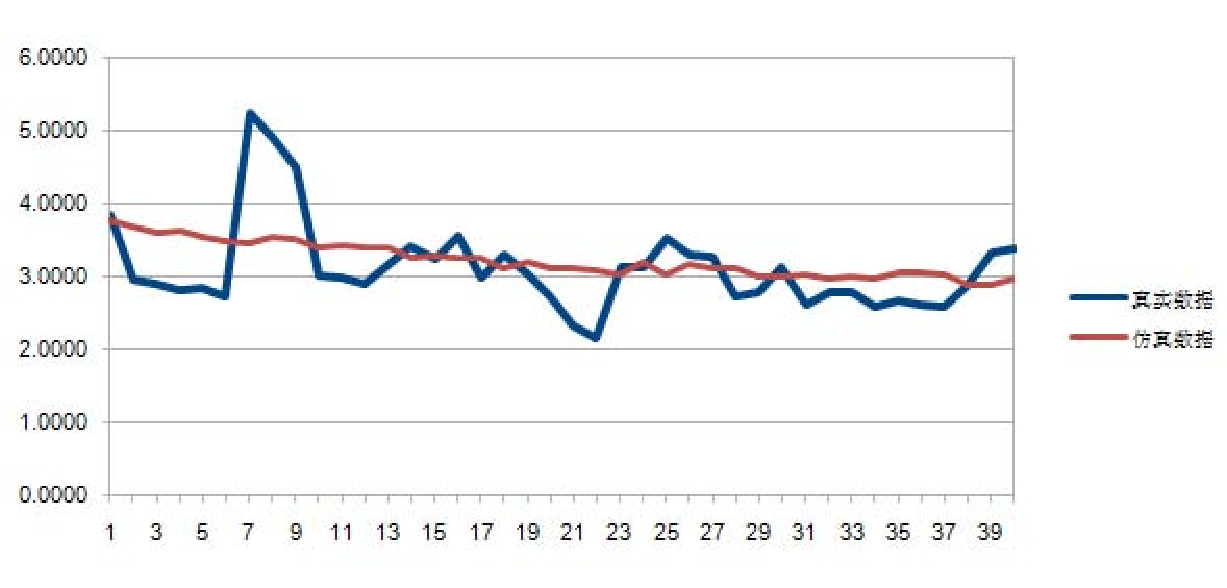
\includegraphics{simu-3.pdf}}
 % GNUPLOT: LaTeX picture
\setlength{\unitlength}{0.240900pt}
\ifx\plotpoint\undefined\newsavebox{\plotpoint}\fi
\begin{picture}(1500,900)(0,0)
\sbox{\plotpoint}{\rule[-0.200pt]{0.400pt}{0.400pt}}%
\put(131.0,82.0){\rule[-0.200pt]{4.818pt}{0.400pt}}
\put(111,82){\makebox(0,0)[r]{ 0}}
\put(1419.0,82.0){\rule[-0.200pt]{4.818pt}{0.400pt}}
\put(131.0,212.0){\rule[-0.200pt]{4.818pt}{0.400pt}}
\put(111,212){\makebox(0,0)[r]{ 1}}
\put(1419.0,212.0){\rule[-0.200pt]{4.818pt}{0.400pt}}
\put(131.0,341.0){\rule[-0.200pt]{4.818pt}{0.400pt}}
\put(111,341){\makebox(0,0)[r]{ 2}}
\put(1419.0,341.0){\rule[-0.200pt]{4.818pt}{0.400pt}}
\put(131.0,471.0){\rule[-0.200pt]{4.818pt}{0.400pt}}
\put(111,471){\makebox(0,0)[r]{ 3}}
\put(1419.0,471.0){\rule[-0.200pt]{4.818pt}{0.400pt}}
\put(131.0,600.0){\rule[-0.200pt]{4.818pt}{0.400pt}}
\put(111,600){\makebox(0,0)[r]{ 4}}
\put(1419.0,600.0){\rule[-0.200pt]{4.818pt}{0.400pt}}
\put(131.0,730.0){\rule[-0.200pt]{4.818pt}{0.400pt}}
\put(111,730){\makebox(0,0)[r]{ 5}}
\put(1419.0,730.0){\rule[-0.200pt]{4.818pt}{0.400pt}}
\put(131.0,859.0){\rule[-0.200pt]{4.818pt}{0.400pt}}
\put(111,859){\makebox(0,0)[r]{ 6}}
\put(1419.0,859.0){\rule[-0.200pt]{4.818pt}{0.400pt}}
\put(131.0,82.0){\rule[-0.200pt]{0.400pt}{4.818pt}}
\put(131,41){\makebox(0,0){ 1}}
\put(131.0,839.0){\rule[-0.200pt]{0.400pt}{4.818pt}}
\put(198.0,82.0){\rule[-0.200pt]{0.400pt}{4.818pt}}
\put(198,41){\makebox(0,0){ 3}}
\put(198.0,839.0){\rule[-0.200pt]{0.400pt}{4.818pt}}
\put(265.0,82.0){\rule[-0.200pt]{0.400pt}{4.818pt}}
\put(265,41){\makebox(0,0){ 5}}
\put(265.0,839.0){\rule[-0.200pt]{0.400pt}{4.818pt}}
\put(332.0,82.0){\rule[-0.200pt]{0.400pt}{4.818pt}}
\put(332,41){\makebox(0,0){ 7}}
\put(332.0,839.0){\rule[-0.200pt]{0.400pt}{4.818pt}}
\put(399.0,82.0){\rule[-0.200pt]{0.400pt}{4.818pt}}
\put(399,41){\makebox(0,0){ 9}}
\put(399.0,839.0){\rule[-0.200pt]{0.400pt}{4.818pt}}
\put(466.0,82.0){\rule[-0.200pt]{0.400pt}{4.818pt}}
\put(466,41){\makebox(0,0){ 11}}
\put(466.0,839.0){\rule[-0.200pt]{0.400pt}{4.818pt}}
\put(533.0,82.0){\rule[-0.200pt]{0.400pt}{4.818pt}}
\put(533,41){\makebox(0,0){ 13}}
\put(533.0,839.0){\rule[-0.200pt]{0.400pt}{4.818pt}}
\put(601.0,82.0){\rule[-0.200pt]{0.400pt}{4.818pt}}
\put(601,41){\makebox(0,0){ 15}}
\put(601.0,839.0){\rule[-0.200pt]{0.400pt}{4.818pt}}
\put(668.0,82.0){\rule[-0.200pt]{0.400pt}{4.818pt}}
\put(668,41){\makebox(0,0){ 17}}
\put(668.0,839.0){\rule[-0.200pt]{0.400pt}{4.818pt}}
\put(735.0,82.0){\rule[-0.200pt]{0.400pt}{4.818pt}}
\put(735,41){\makebox(0,0){ 19}}
\put(735.0,839.0){\rule[-0.200pt]{0.400pt}{4.818pt}}
\put(802.0,82.0){\rule[-0.200pt]{0.400pt}{4.818pt}}
\put(802,41){\makebox(0,0){ 21}}
\put(802.0,839.0){\rule[-0.200pt]{0.400pt}{4.818pt}}
\put(869.0,82.0){\rule[-0.200pt]{0.400pt}{4.818pt}}
\put(869,41){\makebox(0,0){ 23}}
\put(869.0,839.0){\rule[-0.200pt]{0.400pt}{4.818pt}}
\put(936.0,82.0){\rule[-0.200pt]{0.400pt}{4.818pt}}
\put(936,41){\makebox(0,0){ 25}}
\put(936.0,839.0){\rule[-0.200pt]{0.400pt}{4.818pt}}
\put(1003.0,82.0){\rule[-0.200pt]{0.400pt}{4.818pt}}
\put(1003,41){\makebox(0,0){ 27}}
\put(1003.0,839.0){\rule[-0.200pt]{0.400pt}{4.818pt}}
\put(1070.0,82.0){\rule[-0.200pt]{0.400pt}{4.818pt}}
\put(1070,41){\makebox(0,0){ 29}}
\put(1070.0,839.0){\rule[-0.200pt]{0.400pt}{4.818pt}}
\put(1137.0,82.0){\rule[-0.200pt]{0.400pt}{4.818pt}}
\put(1137,41){\makebox(0,0){ 31}}
\put(1137.0,839.0){\rule[-0.200pt]{0.400pt}{4.818pt}}
\put(1204.0,82.0){\rule[-0.200pt]{0.400pt}{4.818pt}}
\put(1204,41){\makebox(0,0){ 33}}
\put(1204.0,839.0){\rule[-0.200pt]{0.400pt}{4.818pt}}
\put(1271.0,82.0){\rule[-0.200pt]{0.400pt}{4.818pt}}
\put(1271,41){\makebox(0,0){ 35}}
\put(1271.0,839.0){\rule[-0.200pt]{0.400pt}{4.818pt}}
\put(1338.0,82.0){\rule[-0.200pt]{0.400pt}{4.818pt}}
\put(1338,41){\makebox(0,0){ 37}}
\put(1338.0,839.0){\rule[-0.200pt]{0.400pt}{4.818pt}}
\put(1405.0,82.0){\rule[-0.200pt]{0.400pt}{4.818pt}}
\put(1405,41){\makebox(0,0){ 39}}
\put(1405.0,839.0){\rule[-0.200pt]{0.400pt}{4.818pt}}
\put(131.0,82.0){\rule[-0.200pt]{0.400pt}{187.179pt}}
\put(131.0,82.0){\rule[-0.200pt]{315.097pt}{0.400pt}}
\put(1439.0,82.0){\rule[-0.200pt]{0.400pt}{187.179pt}}
\put(131.0,859.0){\rule[-0.200pt]{315.097pt}{0.400pt}}
\put(30,470){\makebox(0,0){\rotatebox{90}{用户贡献}}}
\put(785,-10){\makebox(0,0){月度}}
\put(1279,819){\makebox(0,0)[r]{仿真数据}}
\put(1299.0,819.0){\rule[-0.200pt]{24.090pt}{0.400pt}}
\put(1439,547){\usebox{\plotpoint}}
\multiput(1424.47,545.94)(-4.868,-0.468){5}{\rule{3.500pt}{0.113pt}}
\multiput(1431.74,546.17)(-26.736,-4.000){2}{\rule{1.750pt}{0.400pt}}
\multiput(1393.63,541.93)(-3.604,-0.477){7}{\rule{2.740pt}{0.115pt}}
\multiput(1399.31,542.17)(-27.313,-5.000){2}{\rule{1.370pt}{0.400pt}}
\multiput(1357.47,536.94)(-4.868,-0.468){5}{\rule{3.500pt}{0.113pt}}
\multiput(1364.74,537.17)(-26.736,-4.000){2}{\rule{1.750pt}{0.400pt}}
\multiput(1323.89,532.94)(-4.722,-0.468){5}{\rule{3.400pt}{0.113pt}}
\multiput(1330.94,533.17)(-25.943,-4.000){2}{\rule{1.700pt}{0.400pt}}
\multiput(1290.47,528.94)(-4.868,-0.468){5}{\rule{3.500pt}{0.113pt}}
\multiput(1297.74,529.17)(-26.736,-4.000){2}{\rule{1.750pt}{0.400pt}}
\multiput(1256.89,524.94)(-4.722,-0.468){5}{\rule{3.400pt}{0.113pt}}
\multiput(1263.94,525.17)(-25.943,-4.000){2}{\rule{1.700pt}{0.400pt}}
\multiput(1218.77,520.95)(-7.383,-0.447){3}{\rule{4.633pt}{0.108pt}}
\multiput(1228.38,521.17)(-24.383,-3.000){2}{\rule{2.317pt}{0.400pt}}
\multiput(1189.89,517.94)(-4.722,-0.468){5}{\rule{3.400pt}{0.113pt}}
\multiput(1196.94,518.17)(-25.943,-4.000){2}{\rule{1.700pt}{0.400pt}}
\multiput(1151.77,513.95)(-7.383,-0.447){3}{\rule{4.633pt}{0.108pt}}
\multiput(1161.38,514.17)(-24.383,-3.000){2}{\rule{2.317pt}{0.400pt}}
\multiput(1122.89,510.94)(-4.722,-0.468){5}{\rule{3.400pt}{0.113pt}}
\multiput(1129.94,511.17)(-25.943,-4.000){2}{\rule{1.700pt}{0.400pt}}
\multiput(1084.77,506.95)(-7.383,-0.447){3}{\rule{4.633pt}{0.108pt}}
\multiput(1094.38,507.17)(-24.383,-3.000){2}{\rule{2.317pt}{0.400pt}}
\multiput(1051.32,503.95)(-7.160,-0.447){3}{\rule{4.500pt}{0.108pt}}
\multiput(1060.66,504.17)(-23.660,-3.000){2}{\rule{2.250pt}{0.400pt}}
\multiput(1017.77,500.95)(-7.383,-0.447){3}{\rule{4.633pt}{0.108pt}}
\multiput(1027.38,501.17)(-24.383,-3.000){2}{\rule{2.317pt}{0.400pt}}
\multiput(983.77,497.95)(-7.383,-0.447){3}{\rule{4.633pt}{0.108pt}}
\multiput(993.38,498.17)(-24.383,-3.000){2}{\rule{2.317pt}{0.400pt}}
\multiput(950.32,494.95)(-7.160,-0.447){3}{\rule{4.500pt}{0.108pt}}
\multiput(959.66,495.17)(-23.660,-3.000){2}{\rule{2.250pt}{0.400pt}}
\multiput(916.77,491.95)(-7.383,-0.447){3}{\rule{4.633pt}{0.108pt}}
\multiput(926.38,492.17)(-24.383,-3.000){2}{\rule{2.317pt}{0.400pt}}
\multiput(883.32,488.95)(-7.160,-0.447){3}{\rule{4.500pt}{0.108pt}}
\multiput(892.66,489.17)(-23.660,-3.000){2}{\rule{2.250pt}{0.400pt}}
\put(835,485.17){\rule{6.900pt}{0.400pt}}
\multiput(854.68,486.17)(-19.679,-2.000){2}{\rule{3.450pt}{0.400pt}}
\multiput(816.32,483.95)(-7.160,-0.447){3}{\rule{4.500pt}{0.108pt}}
\multiput(825.66,484.17)(-23.660,-3.000){2}{\rule{2.250pt}{0.400pt}}
\put(768,480.17){\rule{6.900pt}{0.400pt}}
\multiput(787.68,481.17)(-19.679,-2.000){2}{\rule{3.450pt}{0.400pt}}
\multiput(749.32,478.95)(-7.160,-0.447){3}{\rule{4.500pt}{0.108pt}}
\multiput(758.66,479.17)(-23.660,-3.000){2}{\rule{2.250pt}{0.400pt}}
\put(701,475.17){\rule{6.900pt}{0.400pt}}
\multiput(720.68,476.17)(-19.679,-2.000){2}{\rule{3.450pt}{0.400pt}}
\put(668,473.17){\rule{6.700pt}{0.400pt}}
\multiput(687.09,474.17)(-19.094,-2.000){2}{\rule{3.350pt}{0.400pt}}
\put(634,471.17){\rule{6.900pt}{0.400pt}}
\multiput(653.68,472.17)(-19.679,-2.000){2}{\rule{3.450pt}{0.400pt}}
\put(601,469.17){\rule{6.700pt}{0.400pt}}
\multiput(620.09,470.17)(-19.094,-2.000){2}{\rule{3.350pt}{0.400pt}}
\put(567,467.67){\rule{8.191pt}{0.400pt}}
\multiput(584.00,468.17)(-17.000,-1.000){2}{\rule{4.095pt}{0.400pt}}
\put(533,466.17){\rule{6.900pt}{0.400pt}}
\multiput(552.68,467.17)(-19.679,-2.000){2}{\rule{3.450pt}{0.400pt}}
\put(500,464.17){\rule{6.700pt}{0.400pt}}
\multiput(519.09,465.17)(-19.094,-2.000){2}{\rule{3.350pt}{0.400pt}}
\put(466,462.67){\rule{8.191pt}{0.400pt}}
\multiput(483.00,463.17)(-17.000,-1.000){2}{\rule{4.095pt}{0.400pt}}
\put(433,461.67){\rule{7.950pt}{0.400pt}}
\multiput(449.50,462.17)(-16.500,-1.000){2}{\rule{3.975pt}{0.400pt}}
\put(399,460.17){\rule{6.900pt}{0.400pt}}
\multiput(418.68,461.17)(-19.679,-2.000){2}{\rule{3.450pt}{0.400pt}}
\put(366,458.67){\rule{7.950pt}{0.400pt}}
\multiput(382.50,459.17)(-16.500,-1.000){2}{\rule{3.975pt}{0.400pt}}
\put(332,457.67){\rule{8.191pt}{0.400pt}}
\multiput(349.00,458.17)(-17.000,-1.000){2}{\rule{4.095pt}{0.400pt}}
\put(299,456.67){\rule{7.950pt}{0.400pt}}
\multiput(315.50,457.17)(-16.500,-1.000){2}{\rule{3.975pt}{0.400pt}}
\put(265,455.67){\rule{8.191pt}{0.400pt}}
\multiput(282.00,456.17)(-17.000,-1.000){2}{\rule{4.095pt}{0.400pt}}
\put(198,454.67){\rule{8.191pt}{0.400pt}}
\multiput(215.00,455.17)(-17.000,-1.000){2}{\rule{4.095pt}{0.400pt}}
\put(232.0,456.0){\rule[-0.200pt]{7.950pt}{0.400pt}}
\put(131,453.67){\rule{8.191pt}{0.400pt}}
\multiput(148.00,454.17)(-17.000,-1.000){2}{\rule{4.095pt}{0.400pt}}
\put(165.0,455.0){\rule[-0.200pt]{7.950pt}{0.400pt}}
\put(1279,768){\makebox(0,0)[r]{实际数据}}
\put(1299.0,768.0){\rule[-0.200pt]{24.090pt}{0.400pt}}
\put(1439,581){\usebox{\plotpoint}}
\multiput(1434.55,581.58)(-1.231,0.494){25}{\rule{1.071pt}{0.119pt}}
\multiput(1436.78,580.17)(-31.776,14.000){2}{\rule{0.536pt}{0.400pt}}
\multiput(1396.76,593.93)(-2.476,-0.485){11}{\rule{1.986pt}{0.117pt}}
\multiput(1400.88,594.17)(-28.879,-7.000){2}{\rule{0.993pt}{0.400pt}}
\multiput(1366.88,586.92)(-1.444,-0.492){21}{\rule{1.233pt}{0.119pt}}
\multiput(1369.44,587.17)(-31.440,-12.000){2}{\rule{0.617pt}{0.400pt}}
\multiput(1319.32,576.61)(-7.160,0.447){3}{\rule{4.500pt}{0.108pt}}
\multiput(1328.66,575.17)(-23.660,3.000){2}{\rule{2.250pt}{0.400pt}}
\multiput(1300.55,577.92)(-1.231,-0.494){25}{\rule{1.071pt}{0.119pt}}
\multiput(1302.78,578.17)(-31.776,-14.000){2}{\rule{0.536pt}{0.400pt}}
\multiput(1269.92,565.00)(-0.497,1.035){63}{\rule{0.120pt}{0.924pt}}
\multiput(1270.17,565.00)(-33.000,66.082){2}{\rule{0.400pt}{0.462pt}}
\multiput(1236.92,633.00)(-0.498,0.856){65}{\rule{0.120pt}{0.782pt}}
\multiput(1237.17,633.00)(-34.000,56.376){2}{\rule{0.400pt}{0.391pt}}
\multiput(1201.39,689.92)(-0.661,-0.497){47}{\rule{0.628pt}{0.120pt}}
\multiput(1202.70,690.17)(-31.697,-25.000){2}{\rule{0.314pt}{0.400pt}}
\multiput(1169.92,658.70)(-0.498,-2.089){65}{\rule{0.120pt}{1.759pt}}
\multiput(1170.17,662.35)(-34.000,-137.349){2}{\rule{0.400pt}{0.879pt}}
\multiput(1135.92,522.47)(-0.497,-0.637){63}{\rule{0.120pt}{0.609pt}}
\multiput(1136.17,523.74)(-33.000,-40.736){2}{\rule{0.400pt}{0.305pt}}
\put(1070,481.67){\rule{8.191pt}{0.400pt}}
\multiput(1087.00,482.17)(-17.000,-1.000){2}{\rule{4.095pt}{0.400pt}}
\multiput(1062.74,482.59)(-2.145,0.488){13}{\rule{1.750pt}{0.117pt}}
\multiput(1066.37,481.17)(-29.368,8.000){2}{\rule{0.875pt}{0.400pt}}
\multiput(1035.92,490.00)(-0.498,0.514){65}{\rule{0.120pt}{0.512pt}}
\multiput(1036.17,490.00)(-34.000,33.938){2}{\rule{0.400pt}{0.256pt}}
\multiput(1000.02,523.92)(-0.775,-0.496){41}{\rule{0.718pt}{0.120pt}}
\multiput(1001.51,524.17)(-32.509,-22.000){2}{\rule{0.359pt}{0.400pt}}
\multiput(967.92,503.00)(-0.497,0.621){63}{\rule{0.120pt}{0.597pt}}
\multiput(968.17,503.00)(-33.000,39.761){2}{\rule{0.400pt}{0.298pt}}
\multiput(934.92,539.82)(-0.498,-1.138){65}{\rule{0.120pt}{1.006pt}}
\multiput(935.17,541.91)(-34.000,-74.912){2}{\rule{0.400pt}{0.503pt}}
\multiput(900.92,467.00)(-0.497,0.637){63}{\rule{0.120pt}{0.609pt}}
\multiput(901.17,467.00)(-33.000,40.736){2}{\rule{0.400pt}{0.305pt}}
\multiput(866.82,507.92)(-0.530,-0.497){61}{\rule{0.525pt}{0.120pt}}
\multiput(867.91,508.17)(-32.910,-32.000){2}{\rule{0.263pt}{0.400pt}}
\multiput(833.92,474.52)(-0.497,-0.621){63}{\rule{0.120pt}{0.597pt}}
\multiput(834.17,475.76)(-33.000,-39.761){2}{\rule{0.400pt}{0.298pt}}
\multiput(800.92,433.05)(-0.498,-0.766){65}{\rule{0.120pt}{0.712pt}}
\multiput(801.17,434.52)(-34.000,-50.523){2}{\rule{0.400pt}{0.356pt}}
\multiput(765.20,382.92)(-0.719,-0.496){43}{\rule{0.674pt}{0.120pt}}
\multiput(766.60,383.17)(-31.601,-23.000){2}{\rule{0.337pt}{0.400pt}}
\multiput(733.92,361.00)(-0.498,1.851){65}{\rule{0.120pt}{1.571pt}}
\multiput(734.17,361.00)(-34.000,121.740){2}{\rule{0.400pt}{0.785pt}}
\put(668,486.17){\rule{6.700pt}{0.400pt}}
\multiput(687.09,485.17)(-19.094,2.000){2}{\rule{3.350pt}{0.400pt}}
\multiput(665.41,488.58)(-0.654,0.497){49}{\rule{0.623pt}{0.120pt}}
\multiput(666.71,487.17)(-32.707,26.000){2}{\rule{0.312pt}{0.400pt}}
\multiput(615.32,512.95)(-7.160,-0.447){3}{\rule{4.500pt}{0.108pt}}
\multiput(624.66,513.17)(-23.660,-3.000){2}{\rule{2.250pt}{0.400pt}}
\multiput(589.29,509.93)(-3.716,-0.477){7}{\rule{2.820pt}{0.115pt}}
\multiput(595.15,510.17)(-28.147,-5.000){2}{\rule{1.410pt}{0.400pt}}
\multiput(565.92,503.39)(-0.498,-0.662){65}{\rule{0.120pt}{0.629pt}}
\multiput(566.17,504.69)(-34.000,-43.694){2}{\rule{0.400pt}{0.315pt}}
\multiput(523.45,461.59)(-2.932,0.482){9}{\rule{2.300pt}{0.116pt}}
\multiput(528.23,460.17)(-28.226,6.000){2}{\rule{1.150pt}{0.400pt}}
\multiput(496.76,467.58)(-0.855,0.496){37}{\rule{0.780pt}{0.119pt}}
\multiput(498.38,466.17)(-32.381,20.000){2}{\rule{0.390pt}{0.400pt}}
\multiput(463.56,485.92)(-0.611,-0.497){51}{\rule{0.589pt}{0.120pt}}
\multiput(464.78,486.17)(-31.778,-27.000){2}{\rule{0.294pt}{0.400pt}}
\multiput(429.61,458.92)(-0.900,-0.495){35}{\rule{0.816pt}{0.119pt}}
\multiput(431.31,459.17)(-32.307,-19.000){2}{\rule{0.408pt}{0.400pt}}
\multiput(380.32,441.61)(-7.160,0.447){3}{\rule{4.500pt}{0.108pt}}
\multiput(389.66,440.17)(-23.660,3.000){2}{\rule{2.250pt}{0.400pt}}
\multiput(317.89,442.94)(-4.722,-0.468){5}{\rule{3.400pt}{0.113pt}}
\multiput(324.94,443.17)(-25.943,-4.000){2}{\rule{1.700pt}{0.400pt}}
\multiput(287.29,438.93)(-3.716,-0.477){7}{\rule{2.820pt}{0.115pt}}
\multiput(293.15,439.17)(-28.147,-5.000){2}{\rule{1.410pt}{0.400pt}}
\multiput(261.98,435.58)(-0.789,0.496){39}{\rule{0.729pt}{0.119pt}}
\multiput(263.49,434.17)(-31.488,21.000){2}{\rule{0.364pt}{0.400pt}}
\multiput(212.77,454.95)(-7.383,-0.447){3}{\rule{4.633pt}{0.108pt}}
\multiput(222.38,455.17)(-24.383,-3.000){2}{\rule{2.317pt}{0.400pt}}
\multiput(196.92,453.00)(-0.497,0.912){63}{\rule{0.120pt}{0.827pt}}
\multiput(197.17,453.00)(-33.000,58.283){2}{\rule{0.400pt}{0.414pt}}
\put(332.0,444.0){\rule[-0.200pt]{8.191pt}{0.400pt}}
\put(1439,581){\makebox(0,0){$+$}}
\put(1405,595){\makebox(0,0){$+$}}
\put(1372,588){\makebox(0,0){$+$}}
\put(1338,576){\makebox(0,0){$+$}}
\put(1305,579){\makebox(0,0){$+$}}
\put(1271,565){\makebox(0,0){$+$}}
\put(1238,633){\makebox(0,0){$+$}}
\put(1204,691){\makebox(0,0){$+$}}
\put(1171,666){\makebox(0,0){$+$}}
\put(1137,525){\makebox(0,0){$+$}}
\put(1104,483){\makebox(0,0){$+$}}
\put(1070,482){\makebox(0,0){$+$}}
\put(1037,490){\makebox(0,0){$+$}}
\put(1003,525){\makebox(0,0){$+$}}
\put(969,503){\makebox(0,0){$+$}}
\put(936,544){\makebox(0,0){$+$}}
\put(902,467){\makebox(0,0){$+$}}
\put(869,509){\makebox(0,0){$+$}}
\put(835,477){\makebox(0,0){$+$}}
\put(802,436){\makebox(0,0){$+$}}
\put(768,384){\makebox(0,0){$+$}}
\put(735,361){\makebox(0,0){$+$}}
\put(701,486){\makebox(0,0){$+$}}
\put(668,488){\makebox(0,0){$+$}}
\put(634,514){\makebox(0,0){$+$}}
\put(601,511){\makebox(0,0){$+$}}
\put(567,506){\makebox(0,0){$+$}}
\put(533,461){\makebox(0,0){$+$}}
\put(500,467){\makebox(0,0){$+$}}
\put(466,487){\makebox(0,0){$+$}}
\put(433,460){\makebox(0,0){$+$}}
\put(399,441){\makebox(0,0){$+$}}
\put(366,444){\makebox(0,0){$+$}}
\put(332,444){\makebox(0,0){$+$}}
\put(299,440){\makebox(0,0){$+$}}
\put(265,435){\makebox(0,0){$+$}}
\put(232,456){\makebox(0,0){$+$}}
\put(198,453){\makebox(0,0){$+$}}
\put(165,513){\makebox(0,0){$+$}}
\put(131,513){\makebox(0,0){$+$}}
\put(1349,768){\makebox(0,0){$+$}}
\put(131.0,513.0){\rule[-0.200pt]{8.191pt}{0.400pt}}
\put(131.0,82.0){\rule[-0.200pt]{0.400pt}{187.179pt}}
\put(131.0,82.0){\rule[-0.200pt]{315.097pt}{0.400pt}}
\put(1439.0,82.0){\rule[-0.200pt]{0.400pt}{187.179pt}}
\put(131.0,859.0){\rule[-0.200pt]{315.097pt}{0.400pt}}
\end{picture}
 
  \caption{\small{\textbf{内容贡献者用户仿真结果}}}
  \label{fig:simu3}
\end{figure}

图\ref{fig:simu4}是内容维护者的仿真结果和真实数据图。实际数据显示内容
维护者的月人均贡献很快下滑,随后逐渐平稳,下滑趋势减缓。仿真数据则是一
条对数曲线,除了和个别真实点的数据结果差距很大以外,整体的拟合度很高,
说明模型对于分析内容维护者的行为是有效的。
\begin{figure}[!htb]
  \centering
%  \scalebox{0.65}{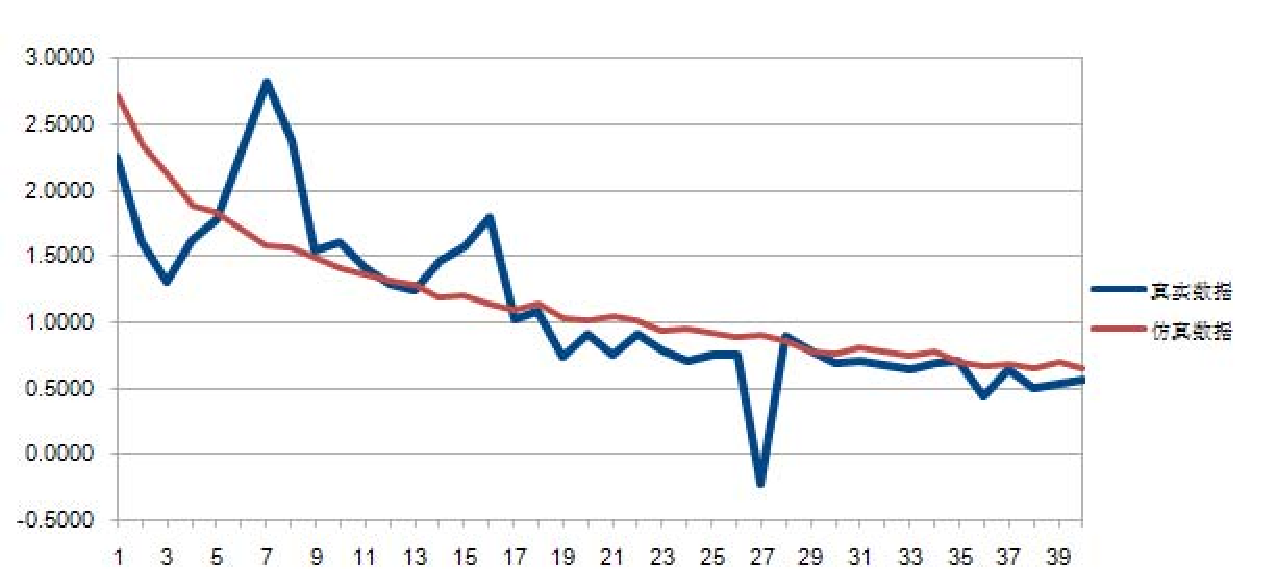
\includegraphics{simu-4.pdf}}
   % GNUPLOT: LaTeX picture
\setlength{\unitlength}{0.240900pt}
\ifx\plotpoint\undefined\newsavebox{\plotpoint}\fi
\begin{picture}(1500,900)(0,0)
\sbox{\plotpoint}{\rule[-0.200pt]{0.400pt}{0.400pt}}%
\put(131.0,82.0){\rule[-0.200pt]{4.818pt}{0.400pt}}
\put(111,82){\makebox(0,0)[r]{-1}}
\put(1419.0,82.0){\rule[-0.200pt]{4.818pt}{0.400pt}}
\put(131.0,237.0){\rule[-0.200pt]{4.818pt}{0.400pt}}
\put(111,237){\makebox(0,0)[r]{ 0}}
\put(1419.0,237.0){\rule[-0.200pt]{4.818pt}{0.400pt}}
\put(131.0,393.0){\rule[-0.200pt]{4.818pt}{0.400pt}}
\put(111,393){\makebox(0,0)[r]{ 1}}
\put(1419.0,393.0){\rule[-0.200pt]{4.818pt}{0.400pt}}
\put(131.0,548.0){\rule[-0.200pt]{4.818pt}{0.400pt}}
\put(111,548){\makebox(0,0)[r]{ 2}}
\put(1419.0,548.0){\rule[-0.200pt]{4.818pt}{0.400pt}}
\put(131.0,704.0){\rule[-0.200pt]{4.818pt}{0.400pt}}
\put(111,704){\makebox(0,0)[r]{ 3}}
\put(1419.0,704.0){\rule[-0.200pt]{4.818pt}{0.400pt}}
\put(131.0,82.0){\rule[-0.200pt]{0.400pt}{4.818pt}}
\put(131,41){\makebox(0,0){ 1}}
\put(131.0,839.0){\rule[-0.200pt]{0.400pt}{4.818pt}}
\put(198.0,82.0){\rule[-0.200pt]{0.400pt}{4.818pt}}
\put(198,41){\makebox(0,0){ 3}}
\put(198.0,839.0){\rule[-0.200pt]{0.400pt}{4.818pt}}
\put(265.0,82.0){\rule[-0.200pt]{0.400pt}{4.818pt}}
\put(265,41){\makebox(0,0){ 5}}
\put(265.0,839.0){\rule[-0.200pt]{0.400pt}{4.818pt}}
\put(332.0,82.0){\rule[-0.200pt]{0.400pt}{4.818pt}}
\put(332,41){\makebox(0,0){ 7}}
\put(332.0,839.0){\rule[-0.200pt]{0.400pt}{4.818pt}}
\put(399.0,82.0){\rule[-0.200pt]{0.400pt}{4.818pt}}
\put(399,41){\makebox(0,0){ 9}}
\put(399.0,839.0){\rule[-0.200pt]{0.400pt}{4.818pt}}
\put(466.0,82.0){\rule[-0.200pt]{0.400pt}{4.818pt}}
\put(466,41){\makebox(0,0){ 11}}
\put(466.0,839.0){\rule[-0.200pt]{0.400pt}{4.818pt}}
\put(533.0,82.0){\rule[-0.200pt]{0.400pt}{4.818pt}}
\put(533,41){\makebox(0,0){ 13}}
\put(533.0,839.0){\rule[-0.200pt]{0.400pt}{4.818pt}}
\put(601.0,82.0){\rule[-0.200pt]{0.400pt}{4.818pt}}
\put(601,41){\makebox(0,0){ 15}}
\put(601.0,839.0){\rule[-0.200pt]{0.400pt}{4.818pt}}
\put(668.0,82.0){\rule[-0.200pt]{0.400pt}{4.818pt}}
\put(668,41){\makebox(0,0){ 17}}
\put(668.0,839.0){\rule[-0.200pt]{0.400pt}{4.818pt}}
\put(735.0,82.0){\rule[-0.200pt]{0.400pt}{4.818pt}}
\put(735,41){\makebox(0,0){ 19}}
\put(735.0,839.0){\rule[-0.200pt]{0.400pt}{4.818pt}}
\put(802.0,82.0){\rule[-0.200pt]{0.400pt}{4.818pt}}
\put(802,41){\makebox(0,0){ 21}}
\put(802.0,839.0){\rule[-0.200pt]{0.400pt}{4.818pt}}
\put(869.0,82.0){\rule[-0.200pt]{0.400pt}{4.818pt}}
\put(869,41){\makebox(0,0){ 23}}
\put(869.0,839.0){\rule[-0.200pt]{0.400pt}{4.818pt}}
\put(936.0,82.0){\rule[-0.200pt]{0.400pt}{4.818pt}}
\put(936,41){\makebox(0,0){ 25}}
\put(936.0,839.0){\rule[-0.200pt]{0.400pt}{4.818pt}}
\put(1003.0,82.0){\rule[-0.200pt]{0.400pt}{4.818pt}}
\put(1003,41){\makebox(0,0){ 27}}
\put(1003.0,839.0){\rule[-0.200pt]{0.400pt}{4.818pt}}
\put(1070.0,82.0){\rule[-0.200pt]{0.400pt}{4.818pt}}
\put(1070,41){\makebox(0,0){ 29}}
\put(1070.0,839.0){\rule[-0.200pt]{0.400pt}{4.818pt}}
\put(1137.0,82.0){\rule[-0.200pt]{0.400pt}{4.818pt}}
\put(1137,41){\makebox(0,0){ 31}}
\put(1137.0,839.0){\rule[-0.200pt]{0.400pt}{4.818pt}}
\put(1204.0,82.0){\rule[-0.200pt]{0.400pt}{4.818pt}}
\put(1204,41){\makebox(0,0){ 33}}
\put(1204.0,839.0){\rule[-0.200pt]{0.400pt}{4.818pt}}
\put(1271.0,82.0){\rule[-0.200pt]{0.400pt}{4.818pt}}
\put(1271,41){\makebox(0,0){ 35}}
\put(1271.0,839.0){\rule[-0.200pt]{0.400pt}{4.818pt}}
\put(1338.0,82.0){\rule[-0.200pt]{0.400pt}{4.818pt}}
\put(1338,41){\makebox(0,0){ 37}}
\put(1338.0,839.0){\rule[-0.200pt]{0.400pt}{4.818pt}}
\put(1405.0,82.0){\rule[-0.200pt]{0.400pt}{4.818pt}}
\put(1405,41){\makebox(0,0){ 39}}
\put(1405.0,839.0){\rule[-0.200pt]{0.400pt}{4.818pt}}
\put(131.0,82.0){\rule[-0.200pt]{0.400pt}{187.179pt}}
\put(131.0,82.0){\rule[-0.200pt]{315.097pt}{0.400pt}}
\put(1439.0,82.0){\rule[-0.200pt]{0.400pt}{187.179pt}}
\put(131.0,859.0){\rule[-0.200pt]{315.097pt}{0.400pt}}
\put(30,470){\makebox(0,0){\rotatebox{90}{用户贡献}}}
\put(1279,819){\makebox(0,0)[r]{仿真数据}}
\put(785,-10){\makebox(0,0){月度}}
\put(1299.0,819.0){\rule[-0.200pt]{24.090pt}{0.400pt}}
\put(131,646){\usebox{\plotpoint}}
\multiput(131.58,643.05)(0.498,-0.766){65}{\rule{0.120pt}{0.712pt}}
\multiput(130.17,644.52)(34.000,-50.523){2}{\rule{0.400pt}{0.356pt}}
\multiput(165.00,592.92)(0.549,-0.497){57}{\rule{0.540pt}{0.120pt}}
\multiput(165.00,593.17)(31.879,-30.000){2}{\rule{0.270pt}{0.400pt}}
\multiput(198.00,562.92)(0.607,-0.497){53}{\rule{0.586pt}{0.120pt}}
\multiput(198.00,563.17)(32.784,-28.000){2}{\rule{0.293pt}{0.400pt}}
\multiput(232.00,534.92)(0.979,-0.495){31}{\rule{0.876pt}{0.119pt}}
\multiput(232.00,535.17)(31.181,-17.000){2}{\rule{0.438pt}{0.400pt}}
\multiput(265.00,517.92)(1.231,-0.494){25}{\rule{1.071pt}{0.119pt}}
\multiput(265.00,518.17)(31.776,-14.000){2}{\rule{0.536pt}{0.400pt}}
\multiput(299.00,503.92)(0.874,-0.495){35}{\rule{0.795pt}{0.119pt}}
\multiput(299.00,504.17)(31.350,-19.000){2}{\rule{0.397pt}{0.400pt}}
\multiput(332.00,484.93)(2.211,-0.488){13}{\rule{1.800pt}{0.117pt}}
\multiput(332.00,485.17)(30.264,-8.000){2}{\rule{0.900pt}{0.400pt}}
\multiput(366.00,476.93)(3.604,-0.477){7}{\rule{2.740pt}{0.115pt}}
\multiput(366.00,477.17)(27.313,-5.000){2}{\rule{1.370pt}{0.400pt}}
\multiput(399.00,471.92)(1.329,-0.493){23}{\rule{1.146pt}{0.119pt}}
\multiput(399.00,472.17)(31.621,-13.000){2}{\rule{0.573pt}{0.400pt}}
\multiput(433.00,458.92)(1.041,-0.494){29}{\rule{0.925pt}{0.119pt}}
\multiput(433.00,459.17)(31.080,-16.000){2}{\rule{0.463pt}{0.400pt}}
\put(466,443.67){\rule{8.191pt}{0.400pt}}
\multiput(466.00,443.17)(17.000,1.000){2}{\rule{4.095pt}{0.400pt}}
\multiput(500.00,443.93)(3.604,-0.477){7}{\rule{2.740pt}{0.115pt}}
\multiput(500.00,444.17)(27.313,-5.000){2}{\rule{1.370pt}{0.400pt}}
\multiput(533.00,438.93)(2.552,-0.485){11}{\rule{2.043pt}{0.117pt}}
\multiput(533.00,439.17)(29.760,-7.000){2}{\rule{1.021pt}{0.400pt}}
\multiput(567.00,431.93)(3.716,-0.477){7}{\rule{2.820pt}{0.115pt}}
\multiput(567.00,432.17)(28.147,-5.000){2}{\rule{1.410pt}{0.400pt}}
\multiput(601.00,426.93)(3.604,-0.477){7}{\rule{2.740pt}{0.115pt}}
\multiput(601.00,427.17)(27.313,-5.000){2}{\rule{1.370pt}{0.400pt}}
\multiput(634.00,421.93)(3.716,-0.477){7}{\rule{2.820pt}{0.115pt}}
\multiput(634.00,422.17)(28.147,-5.000){2}{\rule{1.410pt}{0.400pt}}
\multiput(668.00,416.93)(1.893,-0.489){15}{\rule{1.567pt}{0.118pt}}
\multiput(668.00,417.17)(29.748,-9.000){2}{\rule{0.783pt}{0.400pt}}
\multiput(701.00,407.94)(4.868,-0.468){5}{\rule{3.500pt}{0.113pt}}
\multiput(701.00,408.17)(26.736,-4.000){2}{\rule{1.750pt}{0.400pt}}
\multiput(735.00,403.93)(2.932,-0.482){9}{\rule{2.300pt}{0.116pt}}
\multiput(735.00,404.17)(28.226,-6.000){2}{\rule{1.150pt}{0.400pt}}
\multiput(768.00,397.93)(2.552,-0.485){11}{\rule{2.043pt}{0.117pt}}
\multiput(768.00,398.17)(29.760,-7.000){2}{\rule{1.021pt}{0.400pt}}
\put(802,391.67){\rule{7.950pt}{0.400pt}}
\multiput(802.00,391.17)(16.500,1.000){2}{\rule{3.975pt}{0.400pt}}
\multiput(835.00,391.93)(2.211,-0.488){13}{\rule{1.800pt}{0.117pt}}
\multiput(835.00,392.17)(30.264,-8.000){2}{\rule{0.900pt}{0.400pt}}
\multiput(869.00,383.93)(2.932,-0.482){9}{\rule{2.300pt}{0.116pt}}
\multiput(869.00,384.17)(28.226,-6.000){2}{\rule{1.150pt}{0.400pt}}
\multiput(902.00,377.95)(7.383,-0.447){3}{\rule{4.633pt}{0.108pt}}
\multiput(902.00,378.17)(24.383,-3.000){2}{\rule{2.317pt}{0.400pt}}
\put(936,376.17){\rule{6.700pt}{0.400pt}}
\multiput(936.00,375.17)(19.094,2.000){2}{\rule{3.350pt}{0.400pt}}
\multiput(969.00,376.94)(4.868,-0.468){5}{\rule{3.500pt}{0.113pt}}
\multiput(969.00,377.17)(26.736,-4.000){2}{\rule{1.750pt}{0.400pt}}
\multiput(1003.00,372.93)(2.211,-0.488){13}{\rule{1.800pt}{0.117pt}}
\multiput(1003.00,373.17)(30.264,-8.000){2}{\rule{0.900pt}{0.400pt}}
\multiput(1037.00,364.93)(2.476,-0.485){11}{\rule{1.986pt}{0.117pt}}
\multiput(1037.00,365.17)(28.879,-7.000){2}{\rule{0.993pt}{0.400pt}}
\put(1070,357.67){\rule{8.191pt}{0.400pt}}
\multiput(1070.00,358.17)(17.000,-1.000){2}{\rule{4.095pt}{0.400pt}}
\multiput(1104.00,356.94)(4.722,-0.468){5}{\rule{3.400pt}{0.113pt}}
\multiput(1104.00,357.17)(25.943,-4.000){2}{\rule{1.700pt}{0.400pt}}
\multiput(1137.00,352.94)(4.868,-0.468){5}{\rule{3.500pt}{0.113pt}}
\multiput(1137.00,353.17)(26.736,-4.000){2}{\rule{1.750pt}{0.400pt}}
\put(1171,348.67){\rule{7.950pt}{0.400pt}}
\multiput(1171.00,349.17)(16.500,-1.000){2}{\rule{3.975pt}{0.400pt}}
\put(1238,347.17){\rule{6.700pt}{0.400pt}}
\multiput(1238.00,348.17)(19.094,-2.000){2}{\rule{3.350pt}{0.400pt}}
\put(1271,345.67){\rule{8.191pt}{0.400pt}}
\multiput(1271.00,346.17)(17.000,-1.000){2}{\rule{4.095pt}{0.400pt}}
\put(1305,345.67){\rule{7.950pt}{0.400pt}}
\multiput(1305.00,345.17)(16.500,1.000){2}{\rule{3.975pt}{0.400pt}}
\put(1204.0,349.0){\rule[-0.200pt]{8.191pt}{0.400pt}}
\multiput(1372.00,345.93)(2.476,-0.485){11}{\rule{1.986pt}{0.117pt}}
\multiput(1372.00,346.17)(28.879,-7.000){2}{\rule{0.993pt}{0.400pt}}
\put(1405,338.17){\rule{6.900pt}{0.400pt}}
\multiput(1405.00,339.17)(19.679,-2.000){2}{\rule{3.450pt}{0.400pt}}
\put(1338.0,347.0){\rule[-0.200pt]{8.191pt}{0.400pt}}
\put(1279,768){\makebox(0,0)[r]{实际数据}}
\put(1299.0,768.0){\rule[-0.200pt]{24.090pt}{0.400pt}}
\put(131,587){\usebox{\plotpoint}}
\multiput(131.58,581.75)(0.498,-1.465){65}{\rule{0.120pt}{1.265pt}}
\multiput(130.17,584.38)(34.000,-96.375){2}{\rule{0.400pt}{0.632pt}}
\multiput(165.58,485.12)(0.497,-0.744){63}{\rule{0.120pt}{0.694pt}}
\multiput(164.17,486.56)(33.000,-47.560){2}{\rule{0.400pt}{0.347pt}}
\multiput(198.58,439.00)(0.498,0.751){65}{\rule{0.120pt}{0.700pt}}
\multiput(197.17,439.00)(34.000,49.547){2}{\rule{0.400pt}{0.350pt}}
\multiput(232.00,490.58)(0.719,0.496){43}{\rule{0.674pt}{0.120pt}}
\multiput(232.00,489.17)(31.601,23.000){2}{\rule{0.337pt}{0.400pt}}
\multiput(265.58,513.00)(0.498,1.197){65}{\rule{0.120pt}{1.053pt}}
\multiput(264.17,513.00)(34.000,78.815){2}{\rule{0.400pt}{0.526pt}}
\multiput(299.58,594.00)(0.497,1.265){63}{\rule{0.120pt}{1.106pt}}
\multiput(298.17,594.00)(33.000,80.704){2}{\rule{0.400pt}{0.553pt}}
\multiput(332.58,673.17)(0.498,-1.034){65}{\rule{0.120pt}{0.924pt}}
\multiput(331.17,675.08)(34.000,-68.083){2}{\rule{0.400pt}{0.462pt}}
\multiput(366.58,600.09)(0.497,-1.969){63}{\rule{0.120pt}{1.664pt}}
\multiput(365.17,603.55)(33.000,-125.547){2}{\rule{0.400pt}{0.832pt}}
\multiput(399.00,478.59)(1.951,0.489){15}{\rule{1.611pt}{0.118pt}}
\multiput(399.00,477.17)(30.656,9.000){2}{\rule{0.806pt}{0.400pt}}
\multiput(433.00,485.92)(0.549,-0.497){57}{\rule{0.540pt}{0.120pt}}
\multiput(433.00,486.17)(31.879,-30.000){2}{\rule{0.270pt}{0.400pt}}
\multiput(466.00,455.92)(0.855,-0.496){37}{\rule{0.780pt}{0.119pt}}
\multiput(466.00,456.17)(32.381,-20.000){2}{\rule{0.390pt}{0.400pt}}
\multiput(500.00,435.93)(2.476,-0.485){11}{\rule{1.986pt}{0.117pt}}
\multiput(500.00,436.17)(28.879,-7.000){2}{\rule{0.993pt}{0.400pt}}
\multiput(533.58,430.00)(0.498,0.514){65}{\rule{0.120pt}{0.512pt}}
\multiput(532.17,430.00)(34.000,33.938){2}{\rule{0.400pt}{0.256pt}}
\multiput(567.00,465.58)(1.009,0.495){31}{\rule{0.900pt}{0.119pt}}
\multiput(567.00,464.17)(32.132,17.000){2}{\rule{0.450pt}{0.400pt}}
\multiput(601.58,482.00)(0.497,0.529){63}{\rule{0.120pt}{0.524pt}}
\multiput(600.17,482.00)(33.000,33.912){2}{\rule{0.400pt}{0.262pt}}
\multiput(634.58,510.68)(0.498,-1.792){65}{\rule{0.120pt}{1.524pt}}
\multiput(633.17,513.84)(34.000,-117.838){2}{\rule{0.400pt}{0.762pt}}
\multiput(668.00,396.58)(1.694,0.491){17}{\rule{1.420pt}{0.118pt}}
\multiput(668.00,395.17)(30.053,10.000){2}{\rule{0.710pt}{0.400pt}}
\multiput(701.58,402.95)(0.498,-0.796){65}{\rule{0.120pt}{0.735pt}}
\multiput(700.17,404.47)(34.000,-52.474){2}{\rule{0.400pt}{0.368pt}}
\multiput(735.00,352.58)(0.635,0.497){49}{\rule{0.608pt}{0.120pt}}
\multiput(735.00,351.17)(31.739,26.000){2}{\rule{0.304pt}{0.400pt}}
\multiput(768.00,376.92)(0.775,-0.496){41}{\rule{0.718pt}{0.120pt}}
\multiput(768.00,377.17)(32.509,-22.000){2}{\rule{0.359pt}{0.400pt}}
\multiput(802.00,356.58)(0.752,0.496){41}{\rule{0.700pt}{0.120pt}}
\multiput(802.00,355.17)(31.547,22.000){2}{\rule{0.350pt}{0.400pt}}
\multiput(835.00,376.92)(0.952,-0.495){33}{\rule{0.856pt}{0.119pt}}
\multiput(835.00,377.17)(32.224,-18.000){2}{\rule{0.428pt}{0.400pt}}
\multiput(869.00,358.92)(1.401,-0.492){21}{\rule{1.200pt}{0.119pt}}
\multiput(869.00,359.17)(30.509,-12.000){2}{\rule{0.600pt}{0.400pt}}
\multiput(902.00,348.59)(2.552,0.485){11}{\rule{2.043pt}{0.117pt}}
\multiput(902.00,347.17)(29.760,7.000){2}{\rule{1.021pt}{0.400pt}}
\put(936,354.67){\rule{7.950pt}{0.400pt}}
\multiput(936.00,354.17)(16.500,1.000){2}{\rule{3.975pt}{0.400pt}}
\multiput(969.58,348.11)(0.498,-2.267){65}{\rule{0.120pt}{1.900pt}}
\multiput(968.17,352.06)(34.000,-149.056){2}{\rule{0.400pt}{0.950pt}}
\multiput(1003.58,203.00)(0.498,2.579){65}{\rule{0.120pt}{2.147pt}}
\multiput(1002.17,203.00)(34.000,169.544){2}{\rule{0.400pt}{1.074pt}}
\multiput(1037.00,375.92)(0.923,-0.495){33}{\rule{0.833pt}{0.119pt}}
\multiput(1037.00,376.17)(31.270,-18.000){2}{\rule{0.417pt}{0.400pt}}
\multiput(1070.00,357.92)(1.329,-0.493){23}{\rule{1.146pt}{0.119pt}}
\multiput(1070.00,358.17)(31.621,-13.000){2}{\rule{0.573pt}{0.400pt}}
\put(1104,345.67){\rule{7.950pt}{0.400pt}}
\multiput(1104.00,345.17)(16.500,1.000){2}{\rule{3.975pt}{0.400pt}}
\multiput(1137.00,345.94)(4.868,-0.468){5}{\rule{3.500pt}{0.113pt}}
\multiput(1137.00,346.17)(26.736,-4.000){2}{\rule{1.750pt}{0.400pt}}
\multiput(1171.00,341.93)(3.604,-0.477){7}{\rule{2.740pt}{0.115pt}}
\multiput(1171.00,342.17)(27.313,-5.000){2}{\rule{1.370pt}{0.400pt}}
\multiput(1204.00,338.59)(3.022,0.482){9}{\rule{2.367pt}{0.116pt}}
\multiput(1204.00,337.17)(29.088,6.000){2}{\rule{1.183pt}{0.400pt}}
\multiput(1238.00,344.61)(7.160,0.447){3}{\rule{4.500pt}{0.108pt}}
\multiput(1238.00,343.17)(23.660,3.000){2}{\rule{2.250pt}{0.400pt}}
\multiput(1271.58,344.63)(0.498,-0.588){65}{\rule{0.120pt}{0.571pt}}
\multiput(1270.17,345.82)(34.000,-38.816){2}{\rule{0.400pt}{0.285pt}}
\multiput(1305.00,307.58)(0.531,0.497){59}{\rule{0.526pt}{0.120pt}}
\multiput(1305.00,306.17)(31.909,31.000){2}{\rule{0.263pt}{0.400pt}}
\multiput(1338.00,336.92)(0.741,-0.496){43}{\rule{0.691pt}{0.120pt}}
\multiput(1338.00,337.17)(32.565,-23.000){2}{\rule{0.346pt}{0.400pt}}
\multiput(1372.00,315.59)(2.932,0.482){9}{\rule{2.300pt}{0.116pt}}
\multiput(1372.00,314.17)(28.226,6.000){2}{\rule{1.150pt}{0.400pt}}
\multiput(1405.00,321.60)(4.868,0.468){5}{\rule{3.500pt}{0.113pt}}
\multiput(1405.00,320.17)(26.736,4.000){2}{\rule{1.750pt}{0.400pt}}
\put(131,587){\makebox(0,0){$+$}}
\put(165,488){\makebox(0,0){$+$}}
\put(198,439){\makebox(0,0){$+$}}
\put(232,490){\makebox(0,0){$+$}}
\put(265,513){\makebox(0,0){$+$}}
\put(299,594){\makebox(0,0){$+$}}
\put(332,677){\makebox(0,0){$+$}}
\put(366,607){\makebox(0,0){$+$}}
\put(399,478){\makebox(0,0){$+$}}
\put(433,487){\makebox(0,0){$+$}}
\put(466,457){\makebox(0,0){$+$}}
\put(500,437){\makebox(0,0){$+$}}
\put(533,430){\makebox(0,0){$+$}}
\put(567,465){\makebox(0,0){$+$}}
\put(601,482){\makebox(0,0){$+$}}
\put(634,517){\makebox(0,0){$+$}}
\put(668,396){\makebox(0,0){$+$}}
\put(701,406){\makebox(0,0){$+$}}
\put(735,352){\makebox(0,0){$+$}}
\put(768,378){\makebox(0,0){$+$}}
\put(802,356){\makebox(0,0){$+$}}
\put(835,378){\makebox(0,0){$+$}}
\put(869,360){\makebox(0,0){$+$}}
\put(902,348){\makebox(0,0){$+$}}
\put(936,355){\makebox(0,0){$+$}}
\put(969,356){\makebox(0,0){$+$}}
\put(1003,203){\makebox(0,0){$+$}}
\put(1037,377){\makebox(0,0){$+$}}
\put(1070,359){\makebox(0,0){$+$}}
\put(1104,346){\makebox(0,0){$+$}}
\put(1137,347){\makebox(0,0){$+$}}
\put(1171,343){\makebox(0,0){$+$}}
\put(1204,338){\makebox(0,0){$+$}}
\put(1238,344){\makebox(0,0){$+$}}
\put(1271,347){\makebox(0,0){$+$}}
\put(1305,307){\makebox(0,0){$+$}}
\put(1338,338){\makebox(0,0){$+$}}
\put(1372,315){\makebox(0,0){$+$}}
\put(1405,321){\makebox(0,0){$+$}}
\put(1439,325){\makebox(0,0){$+$}}
\put(1349,768){\makebox(0,0){$+$}}
\put(131.0,82.0){\rule[-0.200pt]{0.400pt}{187.179pt}}
\put(131.0,82.0){\rule[-0.200pt]{315.097pt}{0.400pt}}
\put(1439.0,82.0){\rule[-0.200pt]{0.400pt}{187.179pt}}
\put(131.0,859.0){\rule[-0.200pt]{315.097pt}{0.400pt}}
\end{picture}
 
  \caption{\small{\textbf{内容维护者用户仿真结果}}}
  \label{fig:simu4}
\end{figure}

图\ref{fig:simu5}是边缘用户的仿真结果和真实数据图。边缘用户的月人均贡
献值是所有用户类型中最为特殊的:呈加速下滑趋势。模型仿真结果也显示月人均贡献是一条近
似于指数函数的曲线。虽然真实数据的波动水平比较大,但是模型的拟合结果仍
然反映了真实系统的变动趋势。
\begin{figure}[!htb]
  \centering
%  \scalebox{0.65}{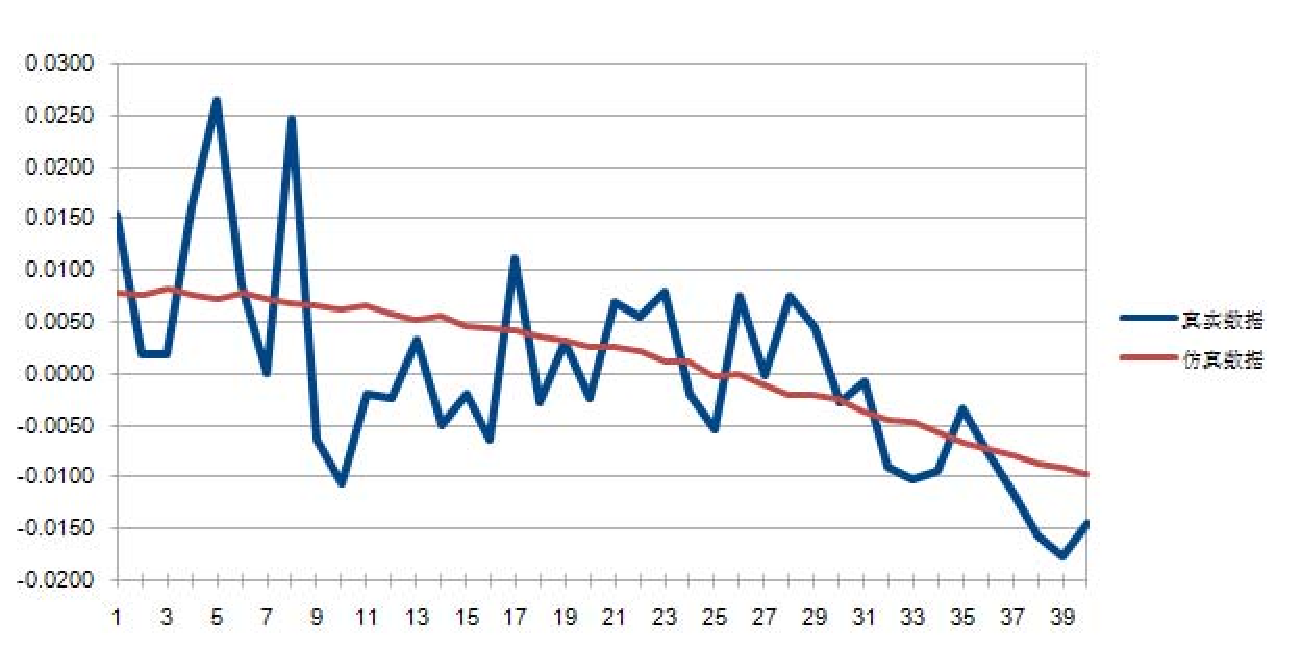
\includegraphics{simu-5.pdf}}
% GNUPLOT: LaTeX picture
\setlength{\unitlength}{0.240900pt}
\ifx\plotpoint\undefined\newsavebox{\plotpoint}\fi
\begin{picture}(1500,900)(0,0)
\sbox{\plotpoint}{\rule[-0.200pt]{0.400pt}{0.400pt}}%
\put(211.0,82.0){\rule[-0.200pt]{4.818pt}{0.400pt}}
\put(191,82){\makebox(0,0)[r]{-0.02}}
\put(1419.0,82.0){\rule[-0.200pt]{4.818pt}{0.400pt}}
\put(211.0,143.0){\rule[-0.200pt]{4.818pt}{0.400pt}}
\put(191,143){\makebox(0,0)[r]{-0.015}}
\put(1419.0,143.0){\rule[-0.200pt]{4.818pt}{0.400pt}}
\put(211.0,203.0){\rule[-0.200pt]{4.818pt}{0.400pt}}
\put(191,203){\makebox(0,0)[r]{-0.01}}
\put(1419.0,203.0){\rule[-0.200pt]{4.818pt}{0.400pt}}
\put(211.0,264.0){\rule[-0.200pt]{4.818pt}{0.400pt}}
\put(191,264){\makebox(0,0)[r]{-0.005}}
\put(1419.0,264.0){\rule[-0.200pt]{4.818pt}{0.400pt}}
\put(211.0,325.0){\rule[-0.200pt]{4.818pt}{0.400pt}}
\put(191,325){\makebox(0,0)[r]{ 0}}
\put(1419.0,325.0){\rule[-0.200pt]{4.818pt}{0.400pt}}
\put(211.0,386.0){\rule[-0.200pt]{4.818pt}{0.400pt}}
\put(191,386){\makebox(0,0)[r]{ 0.005}}
\put(1419.0,386.0){\rule[-0.200pt]{4.818pt}{0.400pt}}
\put(211.0,446.0){\rule[-0.200pt]{4.818pt}{0.400pt}}
\put(191,446){\makebox(0,0)[r]{ 0.01}}
\put(1419.0,446.0){\rule[-0.200pt]{4.818pt}{0.400pt}}
\put(211.0,507.0){\rule[-0.200pt]{4.818pt}{0.400pt}}
\put(191,507){\makebox(0,0)[r]{ 0.015}}
\put(1419.0,507.0){\rule[-0.200pt]{4.818pt}{0.400pt}}
\put(211.0,568.0){\rule[-0.200pt]{4.818pt}{0.400pt}}
\put(191,568){\makebox(0,0)[r]{ 0.02}}
\put(1419.0,568.0){\rule[-0.200pt]{4.818pt}{0.400pt}}
\put(211.0,628.0){\rule[-0.200pt]{4.818pt}{0.400pt}}
\put(191,628){\makebox(0,0)[r]{ 0.025}}
\put(1419.0,628.0){\rule[-0.200pt]{4.818pt}{0.400pt}}
\put(211.0,689.0){\rule[-0.200pt]{4.818pt}{0.400pt}}
\put(191,689){\makebox(0,0)[r]{ 0.03}}
\put(1419.0,689.0){\rule[-0.200pt]{4.818pt}{0.400pt}}
\put(211.0,82.0){\rule[-0.200pt]{0.400pt}{4.818pt}}
\put(211,41){\makebox(0,0){ 1}}
\put(211.0,839.0){\rule[-0.200pt]{0.400pt}{4.818pt}}
\put(274.0,82.0){\rule[-0.200pt]{0.400pt}{4.818pt}}
\put(274,41){\makebox(0,0){ 3}}
\put(274.0,839.0){\rule[-0.200pt]{0.400pt}{4.818pt}}
\put(337.0,82.0){\rule[-0.200pt]{0.400pt}{4.818pt}}
\put(337,41){\makebox(0,0){ 5}}
\put(337.0,839.0){\rule[-0.200pt]{0.400pt}{4.818pt}}
\put(400.0,82.0){\rule[-0.200pt]{0.400pt}{4.818pt}}
\put(400,41){\makebox(0,0){ 7}}
\put(400.0,839.0){\rule[-0.200pt]{0.400pt}{4.818pt}}
\put(463.0,82.0){\rule[-0.200pt]{0.400pt}{4.818pt}}
\put(463,41){\makebox(0,0){ 9}}
\put(463.0,839.0){\rule[-0.200pt]{0.400pt}{4.818pt}}
\put(526.0,82.0){\rule[-0.200pt]{0.400pt}{4.818pt}}
\put(526,41){\makebox(0,0){ 11}}
\put(526.0,839.0){\rule[-0.200pt]{0.400pt}{4.818pt}}
\put(589.0,82.0){\rule[-0.200pt]{0.400pt}{4.818pt}}
\put(589,41){\makebox(0,0){ 13}}
\put(589.0,839.0){\rule[-0.200pt]{0.400pt}{4.818pt}}
\put(652.0,82.0){\rule[-0.200pt]{0.400pt}{4.818pt}}
\put(652,41){\makebox(0,0){ 15}}
\put(652.0,839.0){\rule[-0.200pt]{0.400pt}{4.818pt}}
\put(715.0,82.0){\rule[-0.200pt]{0.400pt}{4.818pt}}
\put(715,41){\makebox(0,0){ 17}}
\put(715.0,839.0){\rule[-0.200pt]{0.400pt}{4.818pt}}
\put(778.0,82.0){\rule[-0.200pt]{0.400pt}{4.818pt}}
\put(778,41){\makebox(0,0){ 19}}
\put(778.0,839.0){\rule[-0.200pt]{0.400pt}{4.818pt}}
\put(841.0,82.0){\rule[-0.200pt]{0.400pt}{4.818pt}}
\put(841,41){\makebox(0,0){ 21}}
\put(841.0,839.0){\rule[-0.200pt]{0.400pt}{4.818pt}}
\put(904.0,82.0){\rule[-0.200pt]{0.400pt}{4.818pt}}
\put(904,41){\makebox(0,0){ 23}}
\put(904.0,839.0){\rule[-0.200pt]{0.400pt}{4.818pt}}
\put(967.0,82.0){\rule[-0.200pt]{0.400pt}{4.818pt}}
\put(967,41){\makebox(0,0){ 25}}
\put(967.0,839.0){\rule[-0.200pt]{0.400pt}{4.818pt}}
\put(1030.0,82.0){\rule[-0.200pt]{0.400pt}{4.818pt}}
\put(1030,41){\makebox(0,0){ 27}}
\put(1030.0,839.0){\rule[-0.200pt]{0.400pt}{4.818pt}}
\put(1093.0,82.0){\rule[-0.200pt]{0.400pt}{4.818pt}}
\put(1093,41){\makebox(0,0){ 29}}
\put(1093.0,839.0){\rule[-0.200pt]{0.400pt}{4.818pt}}
\put(1156.0,82.0){\rule[-0.200pt]{0.400pt}{4.818pt}}
\put(1156,41){\makebox(0,0){ 31}}
\put(1156.0,839.0){\rule[-0.200pt]{0.400pt}{4.818pt}}
\put(1219.0,82.0){\rule[-0.200pt]{0.400pt}{4.818pt}}
\put(1219,41){\makebox(0,0){ 33}}
\put(1219.0,839.0){\rule[-0.200pt]{0.400pt}{4.818pt}}
\put(1282.0,82.0){\rule[-0.200pt]{0.400pt}{4.818pt}}
\put(1282,41){\makebox(0,0){ 35}}
\put(1282.0,839.0){\rule[-0.200pt]{0.400pt}{4.818pt}}
\put(1345.0,82.0){\rule[-0.200pt]{0.400pt}{4.818pt}}
\put(1345,41){\makebox(0,0){ 37}}
\put(1345.0,839.0){\rule[-0.200pt]{0.400pt}{4.818pt}}
\put(1408.0,82.0){\rule[-0.200pt]{0.400pt}{4.818pt}}
\put(1408,41){\makebox(0,0){ 39}}
\put(1408.0,839.0){\rule[-0.200pt]{0.400pt}{4.818pt}}
\put(211.0,82.0){\rule[-0.200pt]{0.400pt}{187.179pt}}
\put(211.0,82.0){\rule[-0.200pt]{295.825pt}{0.400pt}}
\put(1439.0,82.0){\rule[-0.200pt]{0.400pt}{187.179pt}}
\put(211.0,859.0){\rule[-0.200pt]{295.825pt}{0.400pt}}
\put(30,470){\makebox(0,0){\rotatebox{90}{用户贡献}}}
\put(785,-10){\makebox(0,0){月度}}
\put(1279,819){\makebox(0,0)[r]{仿真数据}}
\put(1299.0,819.0){\rule[-0.200pt]{24.090pt}{0.400pt}}
\put(211,423){\usebox{\plotpoint}}
\put(211,421.17){\rule{6.300pt}{0.400pt}}
\multiput(211.00,422.17)(17.924,-2.000){2}{\rule{3.150pt}{0.400pt}}
\multiput(242.00,419.94)(4.575,-0.468){5}{\rule{3.300pt}{0.113pt}}
\multiput(242.00,420.17)(25.151,-4.000){2}{\rule{1.650pt}{0.400pt}}
\multiput(305.00,415.94)(4.575,-0.468){5}{\rule{3.300pt}{0.113pt}}
\multiput(305.00,416.17)(25.151,-4.000){2}{\rule{1.650pt}{0.400pt}}
\multiput(337.00,413.60)(4.429,0.468){5}{\rule{3.200pt}{0.113pt}}
\multiput(337.00,412.17)(24.358,4.000){2}{\rule{1.600pt}{0.400pt}}
\put(274.0,417.0){\rule[-0.200pt]{7.468pt}{0.400pt}}
\multiput(400.00,415.93)(2.013,-0.488){13}{\rule{1.650pt}{0.117pt}}
\multiput(400.00,416.17)(27.575,-8.000){2}{\rule{0.825pt}{0.400pt}}
\multiput(431.00,407.94)(4.575,-0.468){5}{\rule{3.300pt}{0.113pt}}
\multiput(431.00,408.17)(25.151,-4.000){2}{\rule{1.650pt}{0.400pt}}
\multiput(463.00,403.93)(3.382,-0.477){7}{\rule{2.580pt}{0.115pt}}
\multiput(463.00,404.17)(25.645,-5.000){2}{\rule{1.290pt}{0.400pt}}
\multiput(494.00,400.59)(3.493,0.477){7}{\rule{2.660pt}{0.115pt}}
\multiput(494.00,399.17)(26.479,5.000){2}{\rule{1.330pt}{0.400pt}}
\multiput(526.00,403.93)(3.382,-0.477){7}{\rule{2.580pt}{0.115pt}}
\multiput(526.00,404.17)(25.645,-5.000){2}{\rule{1.290pt}{0.400pt}}
\multiput(557.00,398.93)(2.079,-0.488){13}{\rule{1.700pt}{0.117pt}}
\multiput(557.00,399.17)(28.472,-8.000){2}{\rule{0.850pt}{0.400pt}}
\multiput(589.00,390.93)(3.382,-0.477){7}{\rule{2.580pt}{0.115pt}}
\multiput(589.00,391.17)(25.645,-5.000){2}{\rule{1.290pt}{0.400pt}}
\multiput(620.00,385.94)(4.575,-0.468){5}{\rule{3.300pt}{0.113pt}}
\multiput(620.00,386.17)(25.151,-4.000){2}{\rule{1.650pt}{0.400pt}}
\multiput(652.00,381.93)(2.013,-0.488){13}{\rule{1.650pt}{0.117pt}}
\multiput(652.00,382.17)(27.575,-8.000){2}{\rule{0.825pt}{0.400pt}}
\multiput(683.00,373.95)(6.937,-0.447){3}{\rule{4.367pt}{0.108pt}}
\multiput(683.00,374.17)(22.937,-3.000){2}{\rule{2.183pt}{0.400pt}}
\multiput(715.00,370.93)(3.382,-0.477){7}{\rule{2.580pt}{0.115pt}}
\multiput(715.00,371.17)(25.645,-5.000){2}{\rule{1.290pt}{0.400pt}}
\multiput(746.00,365.93)(1.834,-0.489){15}{\rule{1.522pt}{0.118pt}}
\multiput(746.00,366.17)(28.841,-9.000){2}{\rule{0.761pt}{0.400pt}}
\multiput(778.00,358.60)(4.429,0.468){5}{\rule{3.200pt}{0.113pt}}
\multiput(778.00,357.17)(24.358,4.000){2}{\rule{1.600pt}{0.400pt}}
\multiput(809.00,360.92)(1.250,-0.493){23}{\rule{1.085pt}{0.119pt}}
\multiput(809.00,361.17)(29.749,-13.000){2}{\rule{0.542pt}{0.400pt}}
\multiput(841.00,349.60)(4.429,0.468){5}{\rule{3.200pt}{0.113pt}}
\multiput(841.00,348.17)(24.358,4.000){2}{\rule{1.600pt}{0.400pt}}
\multiput(872.00,351.92)(1.009,-0.494){29}{\rule{0.900pt}{0.119pt}}
\multiput(872.00,352.17)(30.132,-16.000){2}{\rule{0.450pt}{0.400pt}}
\put(904,335.67){\rule{7.468pt}{0.400pt}}
\multiput(904.00,336.17)(15.500,-1.000){2}{\rule{3.734pt}{0.400pt}}
\multiput(935.00,334.93)(2.841,-0.482){9}{\rule{2.233pt}{0.116pt}}
\multiput(935.00,335.17)(27.365,-6.000){2}{\rule{1.117pt}{0.400pt}}
\multiput(967.00,328.92)(1.590,-0.491){17}{\rule{1.340pt}{0.118pt}}
\multiput(967.00,329.17)(28.219,-10.000){2}{\rule{0.670pt}{0.400pt}}
\put(998,318.17){\rule{6.500pt}{0.400pt}}
\multiput(998.00,319.17)(18.509,-2.000){2}{\rule{3.250pt}{0.400pt}}
\multiput(1030.00,316.92)(0.977,-0.494){29}{\rule{0.875pt}{0.119pt}}
\multiput(1030.00,317.17)(29.184,-16.000){2}{\rule{0.438pt}{0.400pt}}
\multiput(1061.00,300.93)(2.079,-0.488){13}{\rule{1.700pt}{0.117pt}}
\multiput(1061.00,301.17)(28.472,-8.000){2}{\rule{0.850pt}{0.400pt}}
\multiput(1093.00,292.93)(2.013,-0.488){13}{\rule{1.650pt}{0.117pt}}
\multiput(1093.00,293.17)(27.575,-8.000){2}{\rule{0.825pt}{0.400pt}}
\put(1124,284.67){\rule{7.709pt}{0.400pt}}
\multiput(1124.00,285.17)(16.000,-1.000){2}{\rule{3.854pt}{0.400pt}}
\multiput(1156.00,283.92)(1.590,-0.491){17}{\rule{1.340pt}{0.118pt}}
\multiput(1156.00,284.17)(28.219,-10.000){2}{\rule{0.670pt}{0.400pt}}
\multiput(1187.00,273.92)(1.642,-0.491){17}{\rule{1.380pt}{0.118pt}}
\multiput(1187.00,274.17)(29.136,-10.000){2}{\rule{0.690pt}{0.400pt}}
\multiput(1219.00,263.95)(6.714,-0.447){3}{\rule{4.233pt}{0.108pt}}
\multiput(1219.00,264.17)(22.214,-3.000){2}{\rule{2.117pt}{0.400pt}}
\multiput(1250.00,260.92)(1.642,-0.491){17}{\rule{1.380pt}{0.118pt}}
\multiput(1250.00,261.17)(29.136,-10.000){2}{\rule{0.690pt}{0.400pt}}
\multiput(1282.00,250.92)(1.439,-0.492){19}{\rule{1.227pt}{0.118pt}}
\multiput(1282.00,251.17)(28.453,-11.000){2}{\rule{0.614pt}{0.400pt}}
\multiput(1313.00,239.92)(1.642,-0.491){17}{\rule{1.380pt}{0.118pt}}
\multiput(1313.00,240.17)(29.136,-10.000){2}{\rule{0.690pt}{0.400pt}}
\multiput(1345.00,229.93)(2.013,-0.488){13}{\rule{1.650pt}{0.117pt}}
\multiput(1345.00,230.17)(27.575,-8.000){2}{\rule{0.825pt}{0.400pt}}
\multiput(1376.00,221.93)(3.493,-0.477){7}{\rule{2.660pt}{0.115pt}}
\multiput(1376.00,222.17)(26.479,-5.000){2}{\rule{1.330pt}{0.400pt}}
\multiput(1408.00,216.92)(1.315,-0.492){21}{\rule{1.133pt}{0.119pt}}
\multiput(1408.00,217.17)(28.648,-12.000){2}{\rule{0.567pt}{0.400pt}}
\put(368.0,417.0){\rule[-0.200pt]{7.709pt}{0.400pt}}
\put(1279,768){\makebox(0,0)[r]{实际数据}}
\put(1299.0,768.0){\rule[-0.200pt]{24.090pt}{0.400pt}}
\put(211,512){\usebox{\plotpoint}}
\multiput(211.58,502.80)(0.497,-2.669){59}{\rule{0.120pt}{2.216pt}}
\multiput(210.17,507.40)(31.000,-159.400){2}{\rule{0.400pt}{1.108pt}}
\multiput(274.58,348.00)(0.497,2.800){59}{\rule{0.120pt}{2.319pt}}
\multiput(273.17,348.00)(31.000,167.186){2}{\rule{0.400pt}{1.160pt}}
\multiput(305.58,520.00)(0.497,1.968){61}{\rule{0.120pt}{1.663pt}}
\multiput(304.17,520.00)(32.000,121.549){2}{\rule{0.400pt}{0.831pt}}
\multiput(337.58,639.44)(0.497,-1.559){59}{\rule{0.120pt}{1.339pt}}
\multiput(336.17,642.22)(31.000,-93.221){2}{\rule{0.400pt}{0.669pt}}
\multiput(368.58,543.24)(0.497,-1.621){61}{\rule{0.120pt}{1.388pt}}
\multiput(367.17,546.12)(32.000,-100.120){2}{\rule{0.400pt}{0.694pt}}
\multiput(400.58,442.10)(0.497,-1.054){59}{\rule{0.120pt}{0.939pt}}
\multiput(399.17,444.05)(31.000,-63.052){2}{\rule{0.400pt}{0.469pt}}
\multiput(431.00,381.58)(0.729,0.496){41}{\rule{0.682pt}{0.120pt}}
\multiput(431.00,380.17)(30.585,22.000){2}{\rule{0.341pt}{0.400pt}}
\multiput(463.58,403.00)(0.497,0.841){59}{\rule{0.120pt}{0.771pt}}
\multiput(462.17,403.00)(31.000,50.400){2}{\rule{0.400pt}{0.385pt}}
\multiput(494.58,449.03)(0.497,-1.684){61}{\rule{0.120pt}{1.438pt}}
\multiput(493.17,452.02)(32.000,-104.016){2}{\rule{0.400pt}{0.719pt}}
\multiput(526.00,348.59)(2.751,0.482){9}{\rule{2.167pt}{0.116pt}}
\multiput(526.00,347.17)(26.503,6.000){2}{\rule{1.083pt}{0.400pt}}
\multiput(557.00,354.58)(1.642,0.491){17}{\rule{1.380pt}{0.118pt}}
\multiput(557.00,353.17)(29.136,10.000){2}{\rule{0.690pt}{0.400pt}}
\multiput(589.00,364.58)(0.778,0.496){37}{\rule{0.720pt}{0.119pt}}
\multiput(589.00,363.17)(29.506,20.000){2}{\rule{0.360pt}{0.400pt}}
\multiput(620.58,381.77)(0.497,-0.546){61}{\rule{0.120pt}{0.538pt}}
\multiput(619.17,382.88)(32.000,-33.884){2}{\rule{0.400pt}{0.269pt}}
\multiput(652.58,349.00)(0.497,0.874){59}{\rule{0.120pt}{0.797pt}}
\multiput(651.17,349.00)(31.000,52.346){2}{\rule{0.400pt}{0.398pt}}
\multiput(683.58,403.00)(0.497,0.910){61}{\rule{0.120pt}{0.825pt}}
\multiput(682.17,403.00)(32.000,56.288){2}{\rule{0.400pt}{0.413pt}}
\multiput(715.58,451.48)(0.497,-2.767){59}{\rule{0.120pt}{2.294pt}}
\multiput(714.17,456.24)(31.000,-165.240){2}{\rule{0.400pt}{1.147pt}}
\multiput(746.58,291.00)(0.497,1.115){61}{\rule{0.120pt}{0.988pt}}
\multiput(745.17,291.00)(32.000,68.950){2}{\rule{0.400pt}{0.494pt}}
\multiput(778.58,358.05)(0.497,-1.070){59}{\rule{0.120pt}{0.952pt}}
\multiput(777.17,360.02)(31.000,-64.025){2}{\rule{0.400pt}{0.476pt}}
\multiput(809.58,296.00)(0.497,1.747){61}{\rule{0.120pt}{1.488pt}}
\multiput(808.17,296.00)(32.000,107.913){2}{\rule{0.400pt}{0.744pt}}
\multiput(841.00,405.92)(1.044,-0.494){27}{\rule{0.927pt}{0.119pt}}
\multiput(841.00,406.17)(29.077,-15.000){2}{\rule{0.463pt}{0.400pt}}
\multiput(872.00,392.58)(0.551,0.497){55}{\rule{0.541pt}{0.120pt}}
\multiput(872.00,391.17)(30.876,29.000){2}{\rule{0.271pt}{0.400pt}}
\multiput(904.58,414.21)(0.497,-1.935){59}{\rule{0.120pt}{1.635pt}}
\multiput(903.17,417.61)(31.000,-115.605){2}{\rule{0.400pt}{0.818pt}}
\multiput(935.58,299.35)(0.497,-0.673){61}{\rule{0.120pt}{0.637pt}}
\multiput(934.17,300.68)(32.000,-41.677){2}{\rule{0.400pt}{0.319pt}}
\multiput(967.58,259.00)(0.497,2.555){59}{\rule{0.120pt}{2.126pt}}
\multiput(966.17,259.00)(31.000,152.588){2}{\rule{0.400pt}{1.063pt}}
\multiput(998.58,410.71)(0.497,-1.478){61}{\rule{0.120pt}{1.275pt}}
\multiput(997.17,413.35)(32.000,-91.354){2}{\rule{0.400pt}{0.638pt}}
\multiput(1030.58,322.00)(0.497,1.543){59}{\rule{0.120pt}{1.326pt}}
\multiput(1029.17,322.00)(31.000,92.248){2}{\rule{0.400pt}{0.663pt}}
\multiput(1061.58,414.61)(0.497,-0.594){61}{\rule{0.120pt}{0.575pt}}
\multiput(1060.17,415.81)(32.000,-36.807){2}{\rule{0.400pt}{0.288pt}}
\multiput(1093.58,373.92)(0.497,-1.412){59}{\rule{0.120pt}{1.223pt}}
\multiput(1092.17,376.46)(31.000,-84.462){2}{\rule{0.400pt}{0.611pt}}
\multiput(1124.00,292.58)(0.668,0.496){45}{\rule{0.633pt}{0.120pt}}
\multiput(1124.00,291.17)(30.685,24.000){2}{\rule{0.317pt}{0.400pt}}
\multiput(1156.58,310.23)(0.497,-1.625){59}{\rule{0.120pt}{1.390pt}}
\multiput(1155.17,313.11)(31.000,-97.114){2}{\rule{0.400pt}{0.695pt}}
\multiput(1187.00,214.92)(1.079,-0.494){27}{\rule{0.953pt}{0.119pt}}
\multiput(1187.00,215.17)(30.021,-15.000){2}{\rule{0.477pt}{0.400pt}}
\multiput(1219.00,201.59)(2.013,0.488){13}{\rule{1.650pt}{0.117pt}}
\multiput(1219.00,200.17)(27.575,8.000){2}{\rule{0.825pt}{0.400pt}}
\multiput(1250.58,209.00)(0.497,1.178){61}{\rule{0.120pt}{1.038pt}}
\multiput(1249.17,209.00)(32.000,72.847){2}{\rule{0.400pt}{0.519pt}}
\multiput(1282.58,280.85)(0.497,-0.825){59}{\rule{0.120pt}{0.758pt}}
\multiput(1281.17,282.43)(31.000,-49.427){2}{\rule{0.400pt}{0.379pt}}
\multiput(1313.58,230.09)(0.497,-0.752){61}{\rule{0.120pt}{0.700pt}}
\multiput(1312.17,231.55)(32.000,-46.547){2}{\rule{0.400pt}{0.350pt}}
\multiput(1345.58,181.85)(0.497,-0.825){59}{\rule{0.120pt}{0.758pt}}
\multiput(1344.17,183.43)(31.000,-49.427){2}{\rule{0.400pt}{0.379pt}}
\multiput(1376.00,132.92)(0.668,-0.496){45}{\rule{0.633pt}{0.120pt}}
\multiput(1376.00,133.17)(30.685,-24.000){2}{\rule{0.317pt}{0.400pt}}
\multiput(1408.58,110.00)(0.497,0.646){59}{\rule{0.120pt}{0.616pt}}
\multiput(1407.17,110.00)(31.000,38.721){2}{\rule{0.400pt}{0.308pt}}
\put(211,512){\makebox(0,0){$+$}}
\put(242,348){\makebox(0,0){$+$}}
\put(274,348){\makebox(0,0){$+$}}
\put(305,520){\makebox(0,0){$+$}}
\put(337,645){\makebox(0,0){$+$}}
\put(368,549){\makebox(0,0){$+$}}
\put(400,446){\makebox(0,0){$+$}}
\put(431,381){\makebox(0,0){$+$}}
\put(463,403){\makebox(0,0){$+$}}
\put(494,455){\makebox(0,0){$+$}}
\put(526,348){\makebox(0,0){$+$}}
\put(557,354){\makebox(0,0){$+$}}
\put(589,364){\makebox(0,0){$+$}}
\put(620,384){\makebox(0,0){$+$}}
\put(652,349){\makebox(0,0){$+$}}
\put(683,403){\makebox(0,0){$+$}}
\put(715,461){\makebox(0,0){$+$}}
\put(746,291){\makebox(0,0){$+$}}
\put(778,362){\makebox(0,0){$+$}}
\put(809,296){\makebox(0,0){$+$}}
\put(841,407){\makebox(0,0){$+$}}
\put(872,392){\makebox(0,0){$+$}}
\put(904,421){\makebox(0,0){$+$}}
\put(935,302){\makebox(0,0){$+$}}
\put(967,259){\makebox(0,0){$+$}}
\put(998,416){\makebox(0,0){$+$}}
\put(1030,322){\makebox(0,0){$+$}}
\put(1061,417){\makebox(0,0){$+$}}
\put(1093,379){\makebox(0,0){$+$}}
\put(1124,292){\makebox(0,0){$+$}}
\put(1156,316){\makebox(0,0){$+$}}
\put(1187,216){\makebox(0,0){$+$}}
\put(1219,201){\makebox(0,0){$+$}}
\put(1250,209){\makebox(0,0){$+$}}
\put(1282,284){\makebox(0,0){$+$}}
\put(1313,233){\makebox(0,0){$+$}}
\put(1345,185){\makebox(0,0){$+$}}
\put(1376,134){\makebox(0,0){$+$}}
\put(1408,110){\makebox(0,0){$+$}}
\put(1439,150){\makebox(0,0){$+$}}
\put(1349,768){\makebox(0,0){$+$}}
\put(242.0,348.0){\rule[-0.200pt]{7.709pt}{0.400pt}}
\put(211.0,82.0){\rule[-0.200pt]{0.400pt}{187.179pt}}
\put(211.0,82.0){\rule[-0.200pt]{295.825pt}{0.400pt}}
\put(1439.0,82.0){\rule[-0.200pt]{0.400pt}{187.179pt}}
\put(211.0,859.0){\rule[-0.200pt]{295.825pt}{0.400pt}}
\end{picture}

  \caption{\small{\textbf{边缘用户仿真结果}}}
  \label{fig:simu5}
\end{figure}

从历史检验的效果上看,模型对于用户行为水平的变化趋势进行了比较准确的预
测。其中,对于内容贡献者和内容维护者的拟合程度非常高。但是,实际数据中
仍有一些显著的变动未能在仿真结果中体现出来。这主要是由于以下两方面原因
造成的:首先,某些类别的用户数量较少(如领导者)或者参与协同行为次数较
少(如边缘用户)使得群体的行为表现得随机性较强,个体行为的不确定性更容易凸显
出来,对于这种情况,系统动力学模型的预测精度并不高;第二,协同行为不仅
仅受动机因素影响,许多外界的变化因素都可能使用户行为发生改变,这种改变
是突发的,短暂的,难于预测的,因此会使预测值和实际值发生较大的偏离。

\section{敏感性分析}
\label{sec:sensitivity-test}
敏感性检验是确认模型可靠性的重要手段。一般来说,系统动力学模型擅长处理
那些无法实际观测到具体数值的变量,这些变量可以确定大致的变化范围,但是
很难估计精确的数值。因此估计这些变量在其范围内的变化对系统的影响是模型
检验的重要部分。

然而,大量的敏感性分析表明,模型对于大部分参数的变化都是不敏感的,即使
这些参数的变化非常大。因此,敏感性检验更多地是关注那些会改变系统行为,
使行为模式发生变化的参数,既杠杆点。事实上,敏感性分析的两个主要目的就
是:1)加深对模型的理解,促进模型描述从定性到定量;2)进行政策调控仿
真,分析参数变化对系统行为的影响。

根据检验的目的不同,敏感性可以定
义为三种类别:数值敏感性、行为敏感性以及政策敏感性。数值敏感性关注于参
数和模型输出结果的精确性;行为敏感性关注参数值的改变是否会改变系统行
为;政策敏感性则关注当模型假设发生改变时最优策略的变化情况。

在本文中,将重点研究那些可能是系统行为发生改变的参数。模型建立了
动机因素和协同行为的相互关系,因此系统行为的改变就意味着用户的行为模式
发生了改变,既用户从一种类型变为另一种类型,这对于社区的运营管理者非常
重要。因为这意味着用户从低级用户到优质用户的转变成为可能,通过采取一定
的措施,可以促进用户的转化,从而提升整个社区的质量。

由于系统对于大多数参数是不敏感的,因此对所有的参数进行敏感性分析是不必
要的。针对不同参数的敏感程度排序,快速筛选出那些最敏感、可能改变系统行
为的变量是非常重要的。Ford和Flynn提出使用Pearson相关分析进行进行快速筛
选。通过计算模型参数与输出结果之间的Pearson相关系数,选择系数较大的参
数进行敏感性分析。相关系数越大,说明参数对于输出结果的影响越大,其变化
越有可能改变系统行为。一般来讲,最好考虑相关系数$|r|>0.5$的参数。最终进行分析的参数如下:

\begin{enumerate}
\item 领导者用户。没有符合条件的参数,既模型对于所有动机因素的变化均不
  敏感。
\item 领域专家用户。成就需求是协同行为的主要影响因素,将分析其变化对模
  型的影响。
\item 内容贡献者。没有符合条件的参数,既模型对于所有动机因素的变化均不
  敏感。
\item 内容维护者。自我效能和认知失调是协同行为的主要影响因素,将分析其变化对模
  型的影响。
\item 边缘用户。自我效能和归属感是协同行为的主要影响因素,将分析其变化对模
  型的影响。
\end{enumerate}

选择了需要进行敏感性分析的参数后,将结合政策分析研究起对协同行为的影响。

\section{动机因素模型政策分析}
通过对比模型仿真结果和实际数据,可以判定模型基本反映了维基百科社区中各
类用户的知识协同动机和行为间的关系。利用仿真模型可以进一步分析用户的协
同模式、预测协同行为、分析不同的政策对于用户行为的影响。

\subsection{领导者用户}

领导者用户是整个用户群体中最积极、投入程度最高的群体。个体的人均贡
献远远要高于其他类型的用户。从图中可以看到,尽管有比较明显的波动,但是
月人均贡献还是接近30。领导者用户能有如此高的行为水平和其很强的参与动机是分
不开的。同时,领导者用户的水平很高,其参与的内容绝大部分都受到了其他用
户的认同。因此,协同行为于协同动机形成了正反馈环,使得领导者用户的月人
居贡献不断提高。但是,依据系统动力学原理,正反馈环所造成的良性循环应该
程指数增长,意味着月人均贡献应该是加速上扬的。但是数据显示,领导者用户
的月人均贡献虽然也在上升,但是上升速度确实不断递减的,到最后几乎停滞下
来。

造成这种情况的原因可能有两个:一种是系统本身的主导反馈是负反馈。同正反
馈不同,负反馈回路追求系统的平衡和停滞,一旦系统发生状态偏离,负反馈回
路将使其回到预定的目标或状态。另一种可能是系统的增长模式为S型增长。S型
增长产生的原因是系统中同时存在多个正反馈回路和负反馈回路。当增长达到一
定程度时,负反馈回路开始发挥作用一致增长,是增长不会一直持续下去。最
后,一个或多个条件约束将使增长停止。

根据领导者用户的行为特征,影响领导者的协同贡献的不太呈现完全的负反馈形
式。由于数据选取的时间段为领导者用户已经参与社区的中后期,考虑到较高的
协同贡献,说明领导者用户的月人均协同贡献应该是S型增长,并且到了增长的
末期。在领导者用户的因果回路图中,个人的最大工作时间回路是一个负反馈回
路。当用户的投入水平不断增强,该回路的作用也越来越明显。不管用户
的动机水平有多高,协同行为水平也不可能突破最大工作时间的限制,这时用户
已经是“心有余而力不足”,最终导致了协同贡
献增长的停滞。

为了验证这一点,本文做了两个仿真实验。首先将所有的用户动机程度提升
$10\%$,如果个体的协同行为已经达到了最大值,那么即使提升个体的协同动机
也不可能使协同贡献得到提升。仿真结果如图\ref{fig:improve1}所示。

\begin{figure}
  \centering
  % GNUPLOT: LaTeX picture
\setlength{\unitlength}{0.240900pt}
\ifx\plotpoint\undefined\newsavebox{\plotpoint}\fi
\sbox{\plotpoint}{\rule[-0.200pt]{0.400pt}{0.400pt}}%
\begin{picture}(1500,900)(0,0)
\sbox{\plotpoint}{\rule[-0.200pt]{0.400pt}{0.400pt}}%
\put(131.0,82.0){\rule[-0.200pt]{4.818pt}{0.400pt}}
\put(111,82){\makebox(0,0)[r]{10}}
\put(1419.0,82.0){\rule[-0.200pt]{4.818pt}{0.400pt}}
\put(131.0,211.0){\rule[-0.200pt]{4.818pt}{0.400pt}}
\put(111,211){\makebox(0,0)[r]{15}}
\put(1419.0,211.0){\rule[-0.200pt]{4.818pt}{0.400pt}}
\put(131.0,341.0){\rule[-0.200pt]{4.818pt}{0.400pt}}
\put(111,341){\makebox(0,0)[r]{20}}
\put(1419.0,341.0){\rule[-0.200pt]{4.818pt}{0.400pt}}
\put(131.0,470.0){\rule[-0.200pt]{4.818pt}{0.400pt}}
\put(111,470){\makebox(0,0)[r]{25}}
\put(1419.0,470.0){\rule[-0.200pt]{4.818pt}{0.400pt}}
\put(131.0,600.0){\rule[-0.200pt]{4.818pt}{0.400pt}}
\put(111,600){\makebox(0,0)[r]{30}}
\put(1419.0,600.0){\rule[-0.200pt]{4.818pt}{0.400pt}}
\put(131.0,729.0){\rule[-0.200pt]{4.818pt}{0.400pt}}
\put(111,729){\makebox(0,0)[r]{35}}
\put(1419.0,729.0){\rule[-0.200pt]{4.818pt}{0.400pt}}
\put(131.0,859.0){\rule[-0.200pt]{4.818pt}{0.400pt}}
\put(111,859){\makebox(0,0)[r]{40}}
\put(1419.0,859.0){\rule[-0.200pt]{4.818pt}{0.400pt}}
\put(131.0,82.0){\rule[-0.200pt]{0.400pt}{4.818pt}}
\put(131,41){\makebox(0,0){ 1}}
\put(131.0,839.0){\rule[-0.200pt]{0.400pt}{4.818pt}}
\put(198.0,82.0){\rule[-0.200pt]{0.400pt}{4.818pt}}
\put(198,41){\makebox(0,0){ 3}}
\put(198.0,839.0){\rule[-0.200pt]{0.400pt}{4.818pt}}
\put(265.0,82.0){\rule[-0.200pt]{0.400pt}{4.818pt}}
\put(265,41){\makebox(0,0){ 5}}
\put(265.0,839.0){\rule[-0.200pt]{0.400pt}{4.818pt}}
\put(332.0,82.0){\rule[-0.200pt]{0.400pt}{4.818pt}}
\put(332,41){\makebox(0,0){ 7}}
\put(332.0,839.0){\rule[-0.200pt]{0.400pt}{4.818pt}}
\put(399.0,82.0){\rule[-0.200pt]{0.400pt}{4.818pt}}
\put(399,41){\makebox(0,0){ 9}}
\put(399.0,839.0){\rule[-0.200pt]{0.400pt}{4.818pt}}
\put(466.0,82.0){\rule[-0.200pt]{0.400pt}{4.818pt}}
\put(466,41){\makebox(0,0){ 11}}
\put(466.0,839.0){\rule[-0.200pt]{0.400pt}{4.818pt}}
\put(533.0,82.0){\rule[-0.200pt]{0.400pt}{4.818pt}}
\put(533,41){\makebox(0,0){ 13}}
\put(533.0,839.0){\rule[-0.200pt]{0.400pt}{4.818pt}}
\put(601.0,82.0){\rule[-0.200pt]{0.400pt}{4.818pt}}
\put(601,41){\makebox(0,0){ 15}}
\put(601.0,839.0){\rule[-0.200pt]{0.400pt}{4.818pt}}
\put(668.0,82.0){\rule[-0.200pt]{0.400pt}{4.818pt}}
\put(668,41){\makebox(0,0){ 17}}
\put(668.0,839.0){\rule[-0.200pt]{0.400pt}{4.818pt}}
\put(735.0,82.0){\rule[-0.200pt]{0.400pt}{4.818pt}}
\put(735,41){\makebox(0,0){ 19}}
\put(735.0,839.0){\rule[-0.200pt]{0.400pt}{4.818pt}}
\put(802.0,82.0){\rule[-0.200pt]{0.400pt}{4.818pt}}
\put(802,41){\makebox(0,0){ 21}}
\put(802.0,839.0){\rule[-0.200pt]{0.400pt}{4.818pt}}
\put(869.0,82.0){\rule[-0.200pt]{0.400pt}{4.818pt}}
\put(869,41){\makebox(0,0){ 23}}
\put(869.0,839.0){\rule[-0.200pt]{0.400pt}{4.818pt}}
\put(936.0,82.0){\rule[-0.200pt]{0.400pt}{4.818pt}}
\put(936,41){\makebox(0,0){ 25}}
\put(936.0,839.0){\rule[-0.200pt]{0.400pt}{4.818pt}}
\put(1003.0,82.0){\rule[-0.200pt]{0.400pt}{4.818pt}}
\put(1003,41){\makebox(0,0){ 27}}
\put(1003.0,839.0){\rule[-0.200pt]{0.400pt}{4.818pt}}
\put(1070.0,82.0){\rule[-0.200pt]{0.400pt}{4.818pt}}
\put(1070,41){\makebox(0,0){ 29}}
\put(1070.0,839.0){\rule[-0.200pt]{0.400pt}{4.818pt}}
\put(1137.0,82.0){\rule[-0.200pt]{0.400pt}{4.818pt}}
\put(1137,41){\makebox(0,0){ 31}}
\put(1137.0,839.0){\rule[-0.200pt]{0.400pt}{4.818pt}}
\put(1204.0,82.0){\rule[-0.200pt]{0.400pt}{4.818pt}}
\put(1204,41){\makebox(0,0){ 33}}
\put(1204.0,839.0){\rule[-0.200pt]{0.400pt}{4.818pt}}
\put(1271.0,82.0){\rule[-0.200pt]{0.400pt}{4.818pt}}
\put(1271,41){\makebox(0,0){ 35}}
\put(1271.0,839.0){\rule[-0.200pt]{0.400pt}{4.818pt}}
\put(1338.0,82.0){\rule[-0.200pt]{0.400pt}{4.818pt}}
\put(1338,41){\makebox(0,0){ 37}}
\put(1338.0,839.0){\rule[-0.200pt]{0.400pt}{4.818pt}}
\put(1405.0,82.0){\rule[-0.200pt]{0.400pt}{4.818pt}}
\put(1405,41){\makebox(0,0){ 39}}
\put(1405.0,839.0){\rule[-0.200pt]{0.400pt}{4.818pt}}
\put(131.0,82.0){\rule[-0.200pt]{0.400pt}{187.179pt}}
\put(131.0,82.0){\rule[-0.200pt]{315.097pt}{0.400pt}}
\put(1439.0,82.0){\rule[-0.200pt]{0.400pt}{187.179pt}}
\put(131.0,859.0){\rule[-0.200pt]{315.097pt}{0.400pt}}
\put(30,470){\makebox(0,0){\rotatebox{90}{用户贡献}}}
\put(1279,819){\makebox(0,0)[r]{仿真数据}}
\put(1299.0,819.0){\rule[-0.200pt]{24.090pt}{0.400pt}}
\put(131,139){\usebox{\plotpoint}}
\multiput(131.58,139.00)(0.498,1.316){65}{\rule{0.120pt}{1.147pt}}
\multiput(130.17,139.00)(34.000,86.619){2}{\rule{0.400pt}{0.574pt}}
\multiput(165.58,228.00)(0.497,0.790){63}{\rule{0.120pt}{0.730pt}}
\multiput(164.17,228.00)(33.000,50.484){2}{\rule{0.400pt}{0.365pt}}
\multiput(198.58,280.00)(0.498,0.543){65}{\rule{0.120pt}{0.535pt}}
\multiput(197.17,280.00)(34.000,35.889){2}{\rule{0.400pt}{0.268pt}}
\multiput(232.00,317.58)(0.568,0.497){55}{\rule{0.555pt}{0.120pt}}
\multiput(232.00,316.17)(31.848,29.000){2}{\rule{0.278pt}{0.400pt}}
\multiput(265.00,346.58)(0.710,0.496){45}{\rule{0.667pt}{0.120pt}}
\multiput(265.00,345.17)(32.616,24.000){2}{\rule{0.333pt}{0.400pt}}
\multiput(299.00,370.58)(0.874,0.495){35}{\rule{0.795pt}{0.119pt}}
\multiput(299.00,369.17)(31.350,19.000){2}{\rule{0.397pt}{0.400pt}}
\multiput(332.00,389.58)(0.952,0.495){33}{\rule{0.856pt}{0.119pt}}
\multiput(332.00,388.17)(32.224,18.000){2}{\rule{0.428pt}{0.400pt}}
\multiput(366.00,407.58)(1.113,0.494){27}{\rule{0.980pt}{0.119pt}}
\multiput(366.00,406.17)(30.966,15.000){2}{\rule{0.490pt}{0.400pt}}
\multiput(399.00,422.58)(1.329,0.493){23}{\rule{1.146pt}{0.119pt}}
\multiput(399.00,421.17)(31.621,13.000){2}{\rule{0.573pt}{0.400pt}}
\multiput(433.00,435.58)(1.290,0.493){23}{\rule{1.115pt}{0.119pt}}
\multiput(433.00,434.17)(30.685,13.000){2}{\rule{0.558pt}{0.400pt}}
\multiput(466.00,448.58)(1.581,0.492){19}{\rule{1.336pt}{0.118pt}}
\multiput(466.00,447.17)(31.226,11.000){2}{\rule{0.668pt}{0.400pt}}
\multiput(500.00,459.58)(1.694,0.491){17}{\rule{1.420pt}{0.118pt}}
\multiput(500.00,458.17)(30.053,10.000){2}{\rule{0.710pt}{0.400pt}}
\multiput(533.00,469.58)(1.746,0.491){17}{\rule{1.460pt}{0.118pt}}
\multiput(533.00,468.17)(30.970,10.000){2}{\rule{0.730pt}{0.400pt}}
\multiput(567.00,479.59)(1.951,0.489){15}{\rule{1.611pt}{0.118pt}}
\multiput(567.00,478.17)(30.656,9.000){2}{\rule{0.806pt}{0.400pt}}
\multiput(601.00,488.59)(2.145,0.488){13}{\rule{1.750pt}{0.117pt}}
\multiput(601.00,487.17)(29.368,8.000){2}{\rule{0.875pt}{0.400pt}}
\multiput(634.00,496.59)(2.211,0.488){13}{\rule{1.800pt}{0.117pt}}
\multiput(634.00,495.17)(30.264,8.000){2}{\rule{0.900pt}{0.400pt}}
\multiput(668.00,504.59)(2.476,0.485){11}{\rule{1.986pt}{0.117pt}}
\multiput(668.00,503.17)(28.879,7.000){2}{\rule{0.993pt}{0.400pt}}
\multiput(701.00,511.59)(2.552,0.485){11}{\rule{2.043pt}{0.117pt}}
\multiput(701.00,510.17)(29.760,7.000){2}{\rule{1.021pt}{0.400pt}}
\multiput(735.00,518.59)(2.476,0.485){11}{\rule{1.986pt}{0.117pt}}
\multiput(735.00,517.17)(28.879,7.000){2}{\rule{0.993pt}{0.400pt}}
\multiput(768.00,525.59)(3.022,0.482){9}{\rule{2.367pt}{0.116pt}}
\multiput(768.00,524.17)(29.088,6.000){2}{\rule{1.183pt}{0.400pt}}
\multiput(802.00,531.59)(2.932,0.482){9}{\rule{2.300pt}{0.116pt}}
\multiput(802.00,530.17)(28.226,6.000){2}{\rule{1.150pt}{0.400pt}}
\multiput(835.00,537.59)(3.022,0.482){9}{\rule{2.367pt}{0.116pt}}
\multiput(835.00,536.17)(29.088,6.000){2}{\rule{1.183pt}{0.400pt}}
\multiput(869.00,543.59)(3.604,0.477){7}{\rule{2.740pt}{0.115pt}}
\multiput(869.00,542.17)(27.313,5.000){2}{\rule{1.370pt}{0.400pt}}
\multiput(902.00,548.59)(3.716,0.477){7}{\rule{2.820pt}{0.115pt}}
\multiput(902.00,547.17)(28.147,5.000){2}{\rule{1.410pt}{0.400pt}}
\multiput(936.00,553.59)(2.932,0.482){9}{\rule{2.300pt}{0.116pt}}
\multiput(936.00,552.17)(28.226,6.000){2}{\rule{1.150pt}{0.400pt}}
\multiput(969.00,559.60)(4.868,0.468){5}{\rule{3.500pt}{0.113pt}}
\multiput(969.00,558.17)(26.736,4.000){2}{\rule{1.750pt}{0.400pt}}
\multiput(1003.00,563.59)(3.716,0.477){7}{\rule{2.820pt}{0.115pt}}
\multiput(1003.00,562.17)(28.147,5.000){2}{\rule{1.410pt}{0.400pt}}
\multiput(1037.00,568.59)(3.604,0.477){7}{\rule{2.740pt}{0.115pt}}
\multiput(1037.00,567.17)(27.313,5.000){2}{\rule{1.370pt}{0.400pt}}
\multiput(1070.00,573.60)(4.868,0.468){5}{\rule{3.500pt}{0.113pt}}
\multiput(1070.00,572.17)(26.736,4.000){2}{\rule{1.750pt}{0.400pt}}
\multiput(1104.00,577.60)(4.722,0.468){5}{\rule{3.400pt}{0.113pt}}
\multiput(1104.00,576.17)(25.943,4.000){2}{\rule{1.700pt}{0.400pt}}
\multiput(1137.00,581.60)(4.868,0.468){5}{\rule{3.500pt}{0.113pt}}
\multiput(1137.00,580.17)(26.736,4.000){2}{\rule{1.750pt}{0.400pt}}
\multiput(1171.00,585.60)(4.722,0.468){5}{\rule{3.400pt}{0.113pt}}
\multiput(1171.00,584.17)(25.943,4.000){2}{\rule{1.700pt}{0.400pt}}
\multiput(1204.00,589.60)(4.868,0.468){5}{\rule{3.500pt}{0.113pt}}
\multiput(1204.00,588.17)(26.736,4.000){2}{\rule{1.750pt}{0.400pt}}
\multiput(1238.00,593.60)(4.722,0.468){5}{\rule{3.400pt}{0.113pt}}
\multiput(1238.00,592.17)(25.943,4.000){2}{\rule{1.700pt}{0.400pt}}
\multiput(1271.00,597.61)(7.383,0.447){3}{\rule{4.633pt}{0.108pt}}
\multiput(1271.00,596.17)(24.383,3.000){2}{\rule{2.317pt}{0.400pt}}
\multiput(1305.00,600.60)(4.722,0.468){5}{\rule{3.400pt}{0.113pt}}
\multiput(1305.00,599.17)(25.943,4.000){2}{\rule{1.700pt}{0.400pt}}
\multiput(1338.00,604.61)(7.383,0.447){3}{\rule{4.633pt}{0.108pt}}
\multiput(1338.00,603.17)(24.383,3.000){2}{\rule{2.317pt}{0.400pt}}
\multiput(1372.00,607.60)(4.722,0.468){5}{\rule{3.400pt}{0.113pt}}
\multiput(1372.00,606.17)(25.943,4.000){2}{\rule{1.700pt}{0.400pt}}
\multiput(1405.00,611.61)(7.383,0.447){3}{\rule{4.633pt}{0.108pt}}
\multiput(1405.00,610.17)(24.383,3.000){2}{\rule{2.317pt}{0.400pt}}
\put(1279,768){\makebox(0,0)[r]{改进数据}}
\put(1299.0,768.0){\rule[-0.200pt]{24.090pt}{0.400pt}}
\put(131,150){\usebox{\plotpoint}}
\multiput(131.58,150.00)(0.498,0.960){65}{\rule{0.120pt}{0.865pt}}
\multiput(130.17,150.00)(34.000,63.205){2}{\rule{0.400pt}{0.432pt}}
\multiput(165.58,215.00)(0.497,0.774){63}{\rule{0.120pt}{0.718pt}}
\multiput(164.17,215.00)(33.000,49.509){2}{\rule{0.400pt}{0.359pt}}
\multiput(198.58,266.00)(0.498,0.930){65}{\rule{0.120pt}{0.841pt}}
\multiput(197.17,266.00)(34.000,61.254){2}{\rule{0.400pt}{0.421pt}}
\multiput(232.00,329.58)(0.661,0.497){47}{\rule{0.628pt}{0.120pt}}
\multiput(232.00,328.17)(31.697,25.000){2}{\rule{0.314pt}{0.400pt}}
\put(265,352.67){\rule{8.191pt}{0.400pt}}
\multiput(265.00,353.17)(17.000,-1.000){2}{\rule{4.095pt}{0.400pt}}
\multiput(299.00,353.58)(0.752,0.496){41}{\rule{0.700pt}{0.120pt}}
\multiput(299.00,352.17)(31.547,22.000){2}{\rule{0.350pt}{0.400pt}}
\multiput(332.58,375.00)(0.498,0.633){65}{\rule{0.120pt}{0.606pt}}
\multiput(331.17,375.00)(34.000,41.742){2}{\rule{0.400pt}{0.303pt}}
\multiput(366.00,416.93)(2.932,-0.482){9}{\rule{2.300pt}{0.116pt}}
\multiput(366.00,417.17)(28.226,-6.000){2}{\rule{1.150pt}{0.400pt}}
\multiput(399.00,412.58)(0.630,0.497){51}{\rule{0.604pt}{0.120pt}}
\multiput(399.00,411.17)(32.747,27.000){2}{\rule{0.302pt}{0.400pt}}
\multiput(433.00,439.58)(0.752,0.496){41}{\rule{0.700pt}{0.120pt}}
\multiput(433.00,438.17)(31.547,22.000){2}{\rule{0.350pt}{0.400pt}}
\multiput(466.00,461.59)(2.552,0.485){11}{\rule{2.043pt}{0.117pt}}
\multiput(466.00,460.17)(29.760,7.000){2}{\rule{1.021pt}{0.400pt}}
\multiput(500.00,468.58)(0.923,0.495){33}{\rule{0.833pt}{0.119pt}}
\multiput(500.00,467.17)(31.270,18.000){2}{\rule{0.417pt}{0.400pt}}
\put(533,484.17){\rule{6.900pt}{0.400pt}}
\multiput(533.00,485.17)(19.679,-2.000){2}{\rule{3.450pt}{0.400pt}}
\multiput(567.00,484.58)(1.746,0.491){17}{\rule{1.460pt}{0.118pt}}
\multiput(567.00,483.17)(30.970,10.000){2}{\rule{0.730pt}{0.400pt}}
\multiput(601.00,492.92)(0.874,-0.495){35}{\rule{0.795pt}{0.119pt}}
\multiput(601.00,493.17)(31.350,-19.000){2}{\rule{0.397pt}{0.400pt}}
\multiput(634.58,475.00)(0.498,0.558){65}{\rule{0.120pt}{0.547pt}}
\multiput(633.17,475.00)(34.000,36.865){2}{\rule{0.400pt}{0.274pt}}
\put(668,511.67){\rule{7.950pt}{0.400pt}}
\multiput(668.00,512.17)(16.500,-1.000){2}{\rule{3.975pt}{0.400pt}}
\multiput(701.00,512.59)(2.552,0.485){11}{\rule{2.043pt}{0.117pt}}
\multiput(701.00,511.17)(29.760,7.000){2}{\rule{1.021pt}{0.400pt}}
\put(735,518.67){\rule{7.950pt}{0.400pt}}
\multiput(735.00,518.17)(16.500,1.000){2}{\rule{3.975pt}{0.400pt}}
\multiput(768.00,520.60)(4.868,0.468){5}{\rule{3.500pt}{0.113pt}}
\multiput(768.00,519.17)(26.736,4.000){2}{\rule{1.750pt}{0.400pt}}
\multiput(802.00,524.58)(0.568,0.497){55}{\rule{0.555pt}{0.120pt}}
\multiput(802.00,523.17)(31.848,29.000){2}{\rule{0.278pt}{0.400pt}}
\multiput(835.00,553.60)(4.868,0.468){5}{\rule{3.500pt}{0.113pt}}
\multiput(835.00,552.17)(26.736,4.000){2}{\rule{1.750pt}{0.400pt}}
\multiput(869.00,557.58)(1.401,0.492){21}{\rule{1.200pt}{0.119pt}}
\multiput(869.00,556.17)(30.509,12.000){2}{\rule{0.600pt}{0.400pt}}
\multiput(902.00,567.93)(1.951,-0.489){15}{\rule{1.611pt}{0.118pt}}
\multiput(902.00,568.17)(30.656,-9.000){2}{\rule{0.806pt}{0.400pt}}
\multiput(936.00,560.58)(1.534,0.492){19}{\rule{1.300pt}{0.118pt}}
\multiput(936.00,559.17)(30.302,11.000){2}{\rule{0.650pt}{0.400pt}}
\multiput(969.00,569.93)(2.211,-0.488){13}{\rule{1.800pt}{0.117pt}}
\multiput(969.00,570.17)(30.264,-8.000){2}{\rule{0.900pt}{0.400pt}}
\multiput(1003.00,563.58)(1.073,0.494){29}{\rule{0.950pt}{0.119pt}}
\multiput(1003.00,562.17)(32.028,16.000){2}{\rule{0.475pt}{0.400pt}}
\multiput(1037.00,579.58)(0.979,0.495){31}{\rule{0.876pt}{0.119pt}}
\multiput(1037.00,578.17)(31.181,17.000){2}{\rule{0.438pt}{0.400pt}}
\multiput(1070.00,596.61)(7.383,0.447){3}{\rule{4.633pt}{0.108pt}}
\multiput(1070.00,595.17)(24.383,3.000){2}{\rule{2.317pt}{0.400pt}}
\multiput(1104.00,597.92)(0.789,-0.496){39}{\rule{0.729pt}{0.119pt}}
\multiput(1104.00,598.17)(31.488,-21.000){2}{\rule{0.364pt}{0.400pt}}
\multiput(1137.00,578.58)(1.746,0.491){17}{\rule{1.460pt}{0.118pt}}
\multiput(1137.00,577.17)(30.970,10.000){2}{\rule{0.730pt}{0.400pt}}
\multiput(1171.00,586.92)(0.979,-0.495){31}{\rule{0.876pt}{0.119pt}}
\multiput(1171.00,587.17)(31.181,-17.000){2}{\rule{0.438pt}{0.400pt}}
\multiput(1204.00,571.58)(0.499,0.498){65}{\rule{0.500pt}{0.120pt}}
\multiput(1204.00,570.17)(32.962,34.000){2}{\rule{0.250pt}{0.400pt}}
\multiput(1238.00,605.58)(1.290,0.493){23}{\rule{1.115pt}{0.119pt}}
\multiput(1238.00,604.17)(30.685,13.000){2}{\rule{0.558pt}{0.400pt}}
\multiput(1271.00,616.92)(1.444,-0.492){21}{\rule{1.233pt}{0.119pt}}
\multiput(1271.00,617.17)(31.440,-12.000){2}{\rule{0.617pt}{0.400pt}}
\put(1305,604.17){\rule{6.700pt}{0.400pt}}
\multiput(1305.00,605.17)(19.094,-2.000){2}{\rule{3.350pt}{0.400pt}}
\multiput(1338.00,604.59)(1.951,0.489){15}{\rule{1.611pt}{0.118pt}}
\multiput(1338.00,603.17)(30.656,9.000){2}{\rule{0.806pt}{0.400pt}}
\multiput(1372.00,613.59)(2.932,0.482){9}{\rule{2.300pt}{0.116pt}}
\multiput(1372.00,612.17)(28.226,6.000){2}{\rule{1.150pt}{0.400pt}}
\put(1405,617.17){\rule{6.900pt}{0.400pt}}
\multiput(1405.00,618.17)(19.679,-2.000){2}{\rule{3.450pt}{0.400pt}}
\put(131,150){\makebox(0,0){$+$}}
\put(165,215){\makebox(0,0){$+$}}
\put(198,266){\makebox(0,0){$+$}}
\put(232,329){\makebox(0,0){$+$}}
\put(265,354){\makebox(0,0){$+$}}
\put(299,353){\makebox(0,0){$+$}}
\put(332,375){\makebox(0,0){$+$}}
\put(366,418){\makebox(0,0){$+$}}
\put(399,412){\makebox(0,0){$+$}}
\put(433,439){\makebox(0,0){$+$}}
\put(466,461){\makebox(0,0){$+$}}
\put(500,468){\makebox(0,0){$+$}}
\put(533,486){\makebox(0,0){$+$}}
\put(567,484){\makebox(0,0){$+$}}
\put(601,494){\makebox(0,0){$+$}}
\put(634,475){\makebox(0,0){$+$}}
\put(668,513){\makebox(0,0){$+$}}
\put(701,512){\makebox(0,0){$+$}}
\put(735,519){\makebox(0,0){$+$}}
\put(768,520){\makebox(0,0){$+$}}
\put(802,524){\makebox(0,0){$+$}}
\put(835,553){\makebox(0,0){$+$}}
\put(869,557){\makebox(0,0){$+$}}
\put(902,569){\makebox(0,0){$+$}}
\put(936,560){\makebox(0,0){$+$}}
\put(969,571){\makebox(0,0){$+$}}
\put(1003,563){\makebox(0,0){$+$}}
\put(1037,579){\makebox(0,0){$+$}}
\put(1070,596){\makebox(0,0){$+$}}
\put(1104,599){\makebox(0,0){$+$}}
\put(1137,578){\makebox(0,0){$+$}}
\put(1171,588){\makebox(0,0){$+$}}
\put(1204,571){\makebox(0,0){$+$}}
\put(1238,605){\makebox(0,0){$+$}}
\put(1271,618){\makebox(0,0){$+$}}
\put(1305,606){\makebox(0,0){$+$}}
\put(1338,604){\makebox(0,0){$+$}}
\put(1372,613){\makebox(0,0){$+$}}
\put(1405,619){\makebox(0,0){$+$}}
\put(1439,617){\makebox(0,0){$+$}}
\put(1349,778){\makebox(0,0){$+$}}
\put(131.0,82.0){\rule[-0.200pt]{0.400pt}{187.179pt}}
\put(131.0,82.0){\rule[-0.200pt]{315.097pt}{0.400pt}}
\put(1439.0,82.0){\rule[-0.200pt]{0.400pt}{187.179pt}}
\put(131.0,859.0){\rule[-0.200pt]{315.097pt}{0.400pt}}
\end{picture}

  \caption{\small{\textbf{提升领导者用户初始动机的仿真结果}}}
  \label{fig:improve1}
\end{figure}

从图中可以看出,领导者用户的月人均协同贡献几乎没有变化,这意味着协同动
机的提升对行为已经不能产生影响。接下来,保持其他条件不变,将个体的最大
工作时间加大$10\%$,尽管这已经同现实情况不相符,但是可以借由模拟观察到
最大工作时间对协同行为的限制。仿真结果如图\ref{fig:improve2}所示。

\begin{figure}
  \centering
  %\scalebox{0.65}{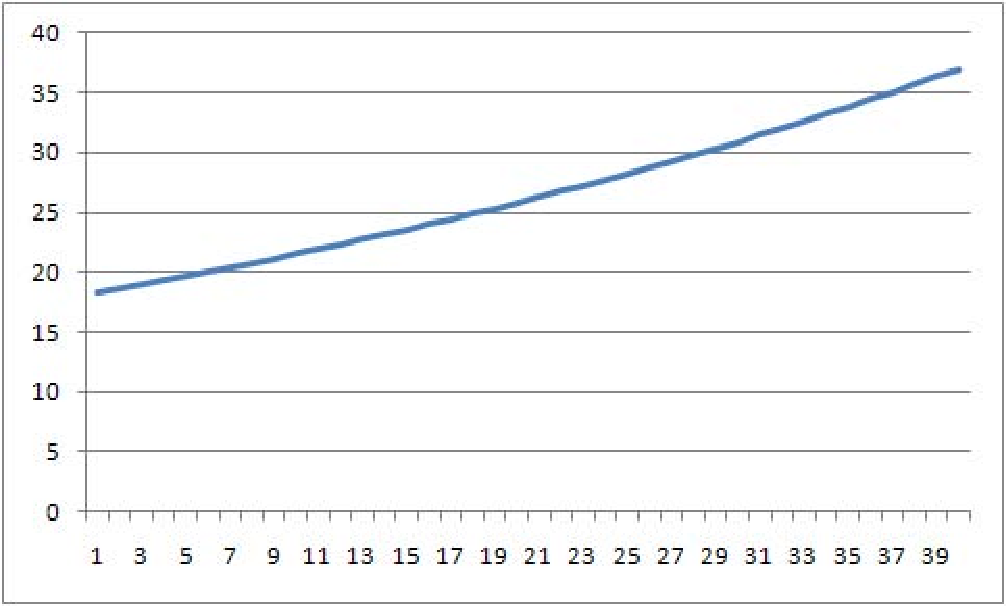
\includegraphics{improve2.pdf}}
% GNUPLOT: LaTeX picture
\setlength{\unitlength}{0.240900pt}
\ifx\plotpoint\undefined\newsavebox{\plotpoint}\fi
\begin{picture}(1500,900)(0,0)
\sbox{\plotpoint}{\rule[-0.200pt]{0.400pt}{0.400pt}}%
\put(131.0,131.0){\rule[-0.200pt]{4.818pt}{0.400pt}}
\put(111,131){\makebox(0,0)[r]{10}}
\put(1419.0,131.0){\rule[-0.200pt]{4.818pt}{0.400pt}}
\put(131.0,252.0){\rule[-0.200pt]{4.818pt}{0.400pt}}
\put(111,252){\makebox(0,0)[r]{15}}
\put(1419.0,252.0){\rule[-0.200pt]{4.818pt}{0.400pt}}
\put(131.0,374.0){\rule[-0.200pt]{4.818pt}{0.400pt}}
\put(111,374){\makebox(0,0)[r]{20}}
\put(1419.0,374.0){\rule[-0.200pt]{4.818pt}{0.400pt}}
\put(131.0,495.0){\rule[-0.200pt]{4.818pt}{0.400pt}}
\put(111,495){\makebox(0,0)[r]{25}}
\put(1419.0,495.0){\rule[-0.200pt]{4.818pt}{0.400pt}}
\put(131.0,616.0){\rule[-0.200pt]{4.818pt}{0.400pt}}
\put(111,616){\makebox(0,0)[r]{30}}
\put(1419.0,616.0){\rule[-0.200pt]{4.818pt}{0.400pt}}
\put(131.0,738.0){\rule[-0.200pt]{4.818pt}{0.400pt}}
\put(111,738){\makebox(0,0)[r]{35}}
\put(1419.0,738.0){\rule[-0.200pt]{4.818pt}{0.400pt}}
\put(131.0,859.0){\rule[-0.200pt]{4.818pt}{0.400pt}}
\put(111,859){\makebox(0,0)[r]{40}}
\put(1419.0,859.0){\rule[-0.200pt]{4.818pt}{0.400pt}}
\put(131.0,131.0){\rule[-0.200pt]{0.400pt}{4.818pt}}
\put(131,90){\makebox(0,0){ 1}}
\put(131.0,839.0){\rule[-0.200pt]{0.400pt}{4.818pt}}
\put(198.0,131.0){\rule[-0.200pt]{0.400pt}{4.818pt}}
\put(198,90){\makebox(0,0){ 3}}
\put(198.0,839.0){\rule[-0.200pt]{0.400pt}{4.818pt}}
\put(265.0,131.0){\rule[-0.200pt]{0.400pt}{4.818pt}}
\put(265,90){\makebox(0,0){ 5}}
\put(265.0,839.0){\rule[-0.200pt]{0.400pt}{4.818pt}}
\put(332.0,131.0){\rule[-0.200pt]{0.400pt}{4.818pt}}
\put(332,90){\makebox(0,0){ 7}}
\put(332.0,839.0){\rule[-0.200pt]{0.400pt}{4.818pt}}
\put(399.0,131.0){\rule[-0.200pt]{0.400pt}{4.818pt}}
\put(399,90){\makebox(0,0){ 9}}
\put(399.0,839.0){\rule[-0.200pt]{0.400pt}{4.818pt}}
\put(466.0,131.0){\rule[-0.200pt]{0.400pt}{4.818pt}}
\put(466,90){\makebox(0,0){ 11}}
\put(466.0,839.0){\rule[-0.200pt]{0.400pt}{4.818pt}}
\put(533.0,131.0){\rule[-0.200pt]{0.400pt}{4.818pt}}
\put(533,90){\makebox(0,0){ 13}}
\put(533.0,839.0){\rule[-0.200pt]{0.400pt}{4.818pt}}
\put(601.0,131.0){\rule[-0.200pt]{0.400pt}{4.818pt}}
\put(601,90){\makebox(0,0){ 15}}
\put(601.0,839.0){\rule[-0.200pt]{0.400pt}{4.818pt}}
\put(668.0,131.0){\rule[-0.200pt]{0.400pt}{4.818pt}}
\put(668,90){\makebox(0,0){ 17}}
\put(668.0,839.0){\rule[-0.200pt]{0.400pt}{4.818pt}}
\put(735.0,131.0){\rule[-0.200pt]{0.400pt}{4.818pt}}
\put(735,90){\makebox(0,0){ 19}}
\put(735.0,839.0){\rule[-0.200pt]{0.400pt}{4.818pt}}
\put(802.0,131.0){\rule[-0.200pt]{0.400pt}{4.818pt}}
\put(802,90){\makebox(0,0){ 21}}
\put(802.0,839.0){\rule[-0.200pt]{0.400pt}{4.818pt}}
\put(869.0,131.0){\rule[-0.200pt]{0.400pt}{4.818pt}}
\put(869,90){\makebox(0,0){ 23}}
\put(869.0,839.0){\rule[-0.200pt]{0.400pt}{4.818pt}}
\put(936.0,131.0){\rule[-0.200pt]{0.400pt}{4.818pt}}
\put(936,90){\makebox(0,0){ 25}}
\put(936.0,839.0){\rule[-0.200pt]{0.400pt}{4.818pt}}
\put(1003.0,131.0){\rule[-0.200pt]{0.400pt}{4.818pt}}
\put(1003,90){\makebox(0,0){ 27}}
\put(1003.0,839.0){\rule[-0.200pt]{0.400pt}{4.818pt}}
\put(1070.0,131.0){\rule[-0.200pt]{0.400pt}{4.818pt}}
\put(1070,90){\makebox(0,0){ 29}}
\put(1070.0,839.0){\rule[-0.200pt]{0.400pt}{4.818pt}}
\put(1137.0,131.0){\rule[-0.200pt]{0.400pt}{4.818pt}}
\put(1137,90){\makebox(0,0){ 31}}
\put(1137.0,839.0){\rule[-0.200pt]{0.400pt}{4.818pt}}
\put(1204.0,131.0){\rule[-0.200pt]{0.400pt}{4.818pt}}
\put(1204,90){\makebox(0,0){ 33}}
\put(1204.0,839.0){\rule[-0.200pt]{0.400pt}{4.818pt}}
\put(1271.0,131.0){\rule[-0.200pt]{0.400pt}{4.818pt}}
\put(1271,90){\makebox(0,0){ 35}}
\put(1271.0,839.0){\rule[-0.200pt]{0.400pt}{4.818pt}}
\put(1338.0,131.0){\rule[-0.200pt]{0.400pt}{4.818pt}}
\put(1338,90){\makebox(0,0){ 37}}
\put(1338.0,839.0){\rule[-0.200pt]{0.400pt}{4.818pt}}
\put(1405.0,131.0){\rule[-0.200pt]{0.400pt}{4.818pt}}
\put(1405,90){\makebox(0,0){ 39}}
\put(1405.0,839.0){\rule[-0.200pt]{0.400pt}{4.818pt}}
\put(131.0,131.0){\rule[-0.200pt]{0.400pt}{175.375pt}}
\put(131.0,131.0){\rule[-0.200pt]{315.097pt}{0.400pt}}
\put(1439.0,131.0){\rule[-0.200pt]{0.400pt}{175.375pt}}
\put(131.0,859.0){\rule[-0.200pt]{315.097pt}{0.400pt}}
\put(30,495){\makebox(0,0){\rotatebox{90}{用户贡献}}}
\put(785,-10){\makebox(0,0){月度}}
\put(1279,819){\makebox(0,0)[r]{仿真数据}}
\put(1299.0,819.0){\rule[-0.200pt]{24.090pt}{0.400pt}}
\put(131,184){\usebox{\plotpoint}}
\multiput(131.58,184.00)(0.498,1.242){65}{\rule{0.120pt}{1.088pt}}
\multiput(130.17,184.00)(34.000,81.741){2}{\rule{0.400pt}{0.544pt}}
\multiput(165.58,268.00)(0.497,0.744){63}{\rule{0.120pt}{0.694pt}}
\multiput(164.17,268.00)(33.000,47.560){2}{\rule{0.400pt}{0.347pt}}
\multiput(198.58,317.00)(0.498,0.514){65}{\rule{0.120pt}{0.512pt}}
\multiput(197.17,317.00)(34.000,33.938){2}{\rule{0.400pt}{0.256pt}}
\multiput(232.00,352.58)(0.635,0.497){49}{\rule{0.608pt}{0.120pt}}
\multiput(232.00,351.17)(31.739,26.000){2}{\rule{0.304pt}{0.400pt}}
\multiput(265.00,378.58)(0.775,0.496){41}{\rule{0.718pt}{0.120pt}}
\multiput(265.00,377.17)(32.509,22.000){2}{\rule{0.359pt}{0.400pt}}
\multiput(299.00,400.58)(0.874,0.495){35}{\rule{0.795pt}{0.119pt}}
\multiput(299.00,399.17)(31.350,19.000){2}{\rule{0.397pt}{0.400pt}}
\multiput(332.00,419.58)(1.073,0.494){29}{\rule{0.950pt}{0.119pt}}
\multiput(332.00,418.17)(32.028,16.000){2}{\rule{0.475pt}{0.400pt}}
\multiput(366.00,435.58)(1.195,0.494){25}{\rule{1.043pt}{0.119pt}}
\multiput(366.00,434.17)(30.835,14.000){2}{\rule{0.521pt}{0.400pt}}
\multiput(399.00,449.58)(1.329,0.493){23}{\rule{1.146pt}{0.119pt}}
\multiput(399.00,448.17)(31.621,13.000){2}{\rule{0.573pt}{0.400pt}}
\multiput(433.00,462.58)(1.401,0.492){21}{\rule{1.200pt}{0.119pt}}
\multiput(433.00,461.17)(30.509,12.000){2}{\rule{0.600pt}{0.400pt}}
\multiput(466.00,474.58)(1.746,0.491){17}{\rule{1.460pt}{0.118pt}}
\multiput(466.00,473.17)(30.970,10.000){2}{\rule{0.730pt}{0.400pt}}
\multiput(500.00,484.58)(1.694,0.491){17}{\rule{1.420pt}{0.118pt}}
\multiput(500.00,483.17)(30.053,10.000){2}{\rule{0.710pt}{0.400pt}}
\multiput(533.00,494.59)(1.951,0.489){15}{\rule{1.611pt}{0.118pt}}
\multiput(533.00,493.17)(30.656,9.000){2}{\rule{0.806pt}{0.400pt}}
\multiput(567.00,503.59)(2.211,0.488){13}{\rule{1.800pt}{0.117pt}}
\multiput(567.00,502.17)(30.264,8.000){2}{\rule{0.900pt}{0.400pt}}
\multiput(601.00,511.59)(2.145,0.488){13}{\rule{1.750pt}{0.117pt}}
\multiput(601.00,510.17)(29.368,8.000){2}{\rule{0.875pt}{0.400pt}}
\multiput(634.00,519.59)(2.552,0.485){11}{\rule{2.043pt}{0.117pt}}
\multiput(634.00,518.17)(29.760,7.000){2}{\rule{1.021pt}{0.400pt}}
\multiput(668.00,526.59)(2.476,0.485){11}{\rule{1.986pt}{0.117pt}}
\multiput(668.00,525.17)(28.879,7.000){2}{\rule{0.993pt}{0.400pt}}
\multiput(701.00,533.59)(2.552,0.485){11}{\rule{2.043pt}{0.117pt}}
\multiput(701.00,532.17)(29.760,7.000){2}{\rule{1.021pt}{0.400pt}}
\multiput(735.00,540.59)(2.932,0.482){9}{\rule{2.300pt}{0.116pt}}
\multiput(735.00,539.17)(28.226,6.000){2}{\rule{1.150pt}{0.400pt}}
\multiput(768.00,546.59)(3.022,0.482){9}{\rule{2.367pt}{0.116pt}}
\multiput(768.00,545.17)(29.088,6.000){2}{\rule{1.183pt}{0.400pt}}
\multiput(802.00,552.59)(3.604,0.477){7}{\rule{2.740pt}{0.115pt}}
\multiput(802.00,551.17)(27.313,5.000){2}{\rule{1.370pt}{0.400pt}}
\multiput(835.00,557.59)(3.022,0.482){9}{\rule{2.367pt}{0.116pt}}
\multiput(835.00,556.17)(29.088,6.000){2}{\rule{1.183pt}{0.400pt}}
\multiput(869.00,563.59)(3.604,0.477){7}{\rule{2.740pt}{0.115pt}}
\multiput(869.00,562.17)(27.313,5.000){2}{\rule{1.370pt}{0.400pt}}
\multiput(902.00,568.59)(3.716,0.477){7}{\rule{2.820pt}{0.115pt}}
\multiput(902.00,567.17)(28.147,5.000){2}{\rule{1.410pt}{0.400pt}}
\multiput(936.00,573.60)(4.722,0.468){5}{\rule{3.400pt}{0.113pt}}
\multiput(936.00,572.17)(25.943,4.000){2}{\rule{1.700pt}{0.400pt}}
\multiput(969.00,577.59)(3.716,0.477){7}{\rule{2.820pt}{0.115pt}}
\multiput(969.00,576.17)(28.147,5.000){2}{\rule{1.410pt}{0.400pt}}
\multiput(1003.00,582.60)(4.868,0.468){5}{\rule{3.500pt}{0.113pt}}
\multiput(1003.00,581.17)(26.736,4.000){2}{\rule{1.750pt}{0.400pt}}
\multiput(1037.00,586.59)(3.604,0.477){7}{\rule{2.740pt}{0.115pt}}
\multiput(1037.00,585.17)(27.313,5.000){2}{\rule{1.370pt}{0.400pt}}
\multiput(1070.00,591.60)(4.868,0.468){5}{\rule{3.500pt}{0.113pt}}
\multiput(1070.00,590.17)(26.736,4.000){2}{\rule{1.750pt}{0.400pt}}
\multiput(1104.00,595.60)(4.722,0.468){5}{\rule{3.400pt}{0.113pt}}
\multiput(1104.00,594.17)(25.943,4.000){2}{\rule{1.700pt}{0.400pt}}
\multiput(1137.00,599.60)(4.868,0.468){5}{\rule{3.500pt}{0.113pt}}
\multiput(1137.00,598.17)(26.736,4.000){2}{\rule{1.750pt}{0.400pt}}
\multiput(1171.00,603.61)(7.160,0.447){3}{\rule{4.500pt}{0.108pt}}
\multiput(1171.00,602.17)(23.660,3.000){2}{\rule{2.250pt}{0.400pt}}
\multiput(1204.00,606.60)(4.868,0.468){5}{\rule{3.500pt}{0.113pt}}
\multiput(1204.00,605.17)(26.736,4.000){2}{\rule{1.750pt}{0.400pt}}
\multiput(1238.00,610.61)(7.160,0.447){3}{\rule{4.500pt}{0.108pt}}
\multiput(1238.00,609.17)(23.660,3.000){2}{\rule{2.250pt}{0.400pt}}
\multiput(1271.00,613.60)(4.868,0.468){5}{\rule{3.500pt}{0.113pt}}
\multiput(1271.00,612.17)(26.736,4.000){2}{\rule{1.750pt}{0.400pt}}
\multiput(1305.00,617.61)(7.160,0.447){3}{\rule{4.500pt}{0.108pt}}
\multiput(1305.00,616.17)(23.660,3.000){2}{\rule{2.250pt}{0.400pt}}
\multiput(1338.00,620.61)(7.383,0.447){3}{\rule{4.633pt}{0.108pt}}
\multiput(1338.00,619.17)(24.383,3.000){2}{\rule{2.317pt}{0.400pt}}
\multiput(1372.00,623.61)(7.160,0.447){3}{\rule{4.500pt}{0.108pt}}
\multiput(1372.00,622.17)(23.660,3.000){2}{\rule{2.250pt}{0.400pt}}
\multiput(1405.00,626.61)(7.383,0.447){3}{\rule{4.633pt}{0.108pt}}
\multiput(1405.00,625.17)(24.383,3.000){2}{\rule{2.317pt}{0.400pt}}
\put(131,184){\makebox(0,0){$+$}}
\put(165,268){\makebox(0,0){$+$}}
\put(198,317){\makebox(0,0){$+$}}
\put(232,352){\makebox(0,0){$+$}}
\put(265,378){\makebox(0,0){$+$}}
\put(299,400){\makebox(0,0){$+$}}
\put(332,419){\makebox(0,0){$+$}}
\put(366,435){\makebox(0,0){$+$}}
\put(399,449){\makebox(0,0){$+$}}
\put(433,462){\makebox(0,0){$+$}}
\put(466,474){\makebox(0,0){$+$}}
\put(500,484){\makebox(0,0){$+$}}
\put(533,494){\makebox(0,0){$+$}}
\put(567,503){\makebox(0,0){$+$}}
\put(601,511){\makebox(0,0){$+$}}
\put(634,519){\makebox(0,0){$+$}}
\put(668,526){\makebox(0,0){$+$}}
\put(701,533){\makebox(0,0){$+$}}
\put(735,540){\makebox(0,0){$+$}}
\put(768,546){\makebox(0,0){$+$}}
\put(802,552){\makebox(0,0){$+$}}
\put(835,557){\makebox(0,0){$+$}}
\put(869,563){\makebox(0,0){$+$}}
\put(902,568){\makebox(0,0){$+$}}
\put(936,573){\makebox(0,0){$+$}}
\put(969,577){\makebox(0,0){$+$}}
\put(1003,582){\makebox(0,0){$+$}}
\put(1037,586){\makebox(0,0){$+$}}
\put(1070,591){\makebox(0,0){$+$}}
\put(1104,595){\makebox(0,0){$+$}}
\put(1137,599){\makebox(0,0){$+$}}
\put(1171,603){\makebox(0,0){$+$}}
\put(1204,606){\makebox(0,0){$+$}}
\put(1238,610){\makebox(0,0){$+$}}
\put(1271,613){\makebox(0,0){$+$}}
\put(1305,617){\makebox(0,0){$+$}}
\put(1338,620){\makebox(0,0){$+$}}
\put(1372,623){\makebox(0,0){$+$}}
\put(1405,626){\makebox(0,0){$+$}}
\put(1439,629){\makebox(0,0){$+$}}
\put(1349,819){\makebox(0,0){$+$}}
\put(1279,768){\makebox(0,0)[r]{改进数据}}
\put(1299.0,768.0){\rule[-0.200pt]{24.090pt}{0.400pt}}
\put(131,333){\usebox{\plotpoint}}
\multiput(131.00,333.59)(2.211,0.488){13}{\rule{1.800pt}{0.117pt}}
\multiput(131.00,332.17)(30.264,8.000){2}{\rule{0.900pt}{0.400pt}}
\multiput(165.00,341.59)(2.145,0.488){13}{\rule{1.750pt}{0.117pt}}
\multiput(165.00,340.17)(29.368,8.000){2}{\rule{0.875pt}{0.400pt}}
\multiput(198.00,349.59)(1.951,0.489){15}{\rule{1.611pt}{0.118pt}}
\multiput(198.00,348.17)(30.656,9.000){2}{\rule{0.806pt}{0.400pt}}
\multiput(232.00,358.59)(2.145,0.488){13}{\rule{1.750pt}{0.117pt}}
\multiput(232.00,357.17)(29.368,8.000){2}{\rule{0.875pt}{0.400pt}}
\multiput(265.00,366.59)(1.951,0.489){15}{\rule{1.611pt}{0.118pt}}
\multiput(265.00,365.17)(30.656,9.000){2}{\rule{0.806pt}{0.400pt}}
\multiput(299.00,375.59)(1.893,0.489){15}{\rule{1.567pt}{0.118pt}}
\multiput(299.00,374.17)(29.748,9.000){2}{\rule{0.783pt}{0.400pt}}
\multiput(332.00,384.59)(1.951,0.489){15}{\rule{1.611pt}{0.118pt}}
\multiput(332.00,383.17)(30.656,9.000){2}{\rule{0.806pt}{0.400pt}}
\multiput(366.00,393.59)(1.893,0.489){15}{\rule{1.567pt}{0.118pt}}
\multiput(366.00,392.17)(29.748,9.000){2}{\rule{0.783pt}{0.400pt}}
\multiput(399.00,402.59)(1.951,0.489){15}{\rule{1.611pt}{0.118pt}}
\multiput(399.00,401.17)(30.656,9.000){2}{\rule{0.806pt}{0.400pt}}
\multiput(433.00,411.58)(1.694,0.491){17}{\rule{1.420pt}{0.118pt}}
\multiput(433.00,410.17)(30.053,10.000){2}{\rule{0.710pt}{0.400pt}}
\multiput(466.00,421.59)(1.951,0.489){15}{\rule{1.611pt}{0.118pt}}
\multiput(466.00,420.17)(30.656,9.000){2}{\rule{0.806pt}{0.400pt}}
\multiput(500.00,430.58)(1.694,0.491){17}{\rule{1.420pt}{0.118pt}}
\multiput(500.00,429.17)(30.053,10.000){2}{\rule{0.710pt}{0.400pt}}
\multiput(533.00,440.58)(1.746,0.491){17}{\rule{1.460pt}{0.118pt}}
\multiput(533.00,439.17)(30.970,10.000){2}{\rule{0.730pt}{0.400pt}}
\multiput(567.00,450.58)(1.581,0.492){19}{\rule{1.336pt}{0.118pt}}
\multiput(567.00,449.17)(31.226,11.000){2}{\rule{0.668pt}{0.400pt}}
\multiput(601.00,461.58)(1.694,0.491){17}{\rule{1.420pt}{0.118pt}}
\multiput(601.00,460.17)(30.053,10.000){2}{\rule{0.710pt}{0.400pt}}
\multiput(634.00,471.58)(1.746,0.491){17}{\rule{1.460pt}{0.118pt}}
\multiput(634.00,470.17)(30.970,10.000){2}{\rule{0.730pt}{0.400pt}}
\multiput(668.00,481.58)(1.534,0.492){19}{\rule{1.300pt}{0.118pt}}
\multiput(668.00,480.17)(30.302,11.000){2}{\rule{0.650pt}{0.400pt}}
\multiput(701.00,492.58)(1.581,0.492){19}{\rule{1.336pt}{0.118pt}}
\multiput(701.00,491.17)(31.226,11.000){2}{\rule{0.668pt}{0.400pt}}
\multiput(735.00,503.58)(1.534,0.492){19}{\rule{1.300pt}{0.118pt}}
\multiput(735.00,502.17)(30.302,11.000){2}{\rule{0.650pt}{0.400pt}}
\multiput(768.00,514.58)(1.444,0.492){21}{\rule{1.233pt}{0.119pt}}
\multiput(768.00,513.17)(31.440,12.000){2}{\rule{0.617pt}{0.400pt}}
\multiput(802.00,526.58)(1.534,0.492){19}{\rule{1.300pt}{0.118pt}}
\multiput(802.00,525.17)(30.302,11.000){2}{\rule{0.650pt}{0.400pt}}
\multiput(835.00,537.58)(1.444,0.492){21}{\rule{1.233pt}{0.119pt}}
\multiput(835.00,536.17)(31.440,12.000){2}{\rule{0.617pt}{0.400pt}}
\multiput(869.00,549.58)(1.401,0.492){21}{\rule{1.200pt}{0.119pt}}
\multiput(869.00,548.17)(30.509,12.000){2}{\rule{0.600pt}{0.400pt}}
\multiput(902.00,561.58)(1.444,0.492){21}{\rule{1.233pt}{0.119pt}}
\multiput(902.00,560.17)(31.440,12.000){2}{\rule{0.617pt}{0.400pt}}
\multiput(936.00,573.58)(1.290,0.493){23}{\rule{1.115pt}{0.119pt}}
\multiput(936.00,572.17)(30.685,13.000){2}{\rule{0.558pt}{0.400pt}}
\multiput(969.00,586.58)(1.444,0.492){21}{\rule{1.233pt}{0.119pt}}
\multiput(969.00,585.17)(31.440,12.000){2}{\rule{0.617pt}{0.400pt}}
\multiput(1003.00,598.58)(1.329,0.493){23}{\rule{1.146pt}{0.119pt}}
\multiput(1003.00,597.17)(31.621,13.000){2}{\rule{0.573pt}{0.400pt}}
\multiput(1037.00,611.58)(1.195,0.494){25}{\rule{1.043pt}{0.119pt}}
\multiput(1037.00,610.17)(30.835,14.000){2}{\rule{0.521pt}{0.400pt}}
\multiput(1070.00,625.58)(1.329,0.493){23}{\rule{1.146pt}{0.119pt}}
\multiput(1070.00,624.17)(31.621,13.000){2}{\rule{0.573pt}{0.400pt}}
\multiput(1104.00,638.58)(1.195,0.494){25}{\rule{1.043pt}{0.119pt}}
\multiput(1104.00,637.17)(30.835,14.000){2}{\rule{0.521pt}{0.400pt}}
\multiput(1137.00,652.58)(1.329,0.493){23}{\rule{1.146pt}{0.119pt}}
\multiput(1137.00,651.17)(31.621,13.000){2}{\rule{0.573pt}{0.400pt}}
\multiput(1171.00,665.58)(1.195,0.494){25}{\rule{1.043pt}{0.119pt}}
\multiput(1171.00,664.17)(30.835,14.000){2}{\rule{0.521pt}{0.400pt}}
\multiput(1204.00,679.58)(1.147,0.494){27}{\rule{1.007pt}{0.119pt}}
\multiput(1204.00,678.17)(31.911,15.000){2}{\rule{0.503pt}{0.400pt}}
\multiput(1238.00,694.58)(1.113,0.494){27}{\rule{0.980pt}{0.119pt}}
\multiput(1238.00,693.17)(30.966,15.000){2}{\rule{0.490pt}{0.400pt}}
\multiput(1271.00,709.58)(1.231,0.494){25}{\rule{1.071pt}{0.119pt}}
\multiput(1271.00,708.17)(31.776,14.000){2}{\rule{0.536pt}{0.400pt}}
\multiput(1305.00,723.58)(1.041,0.494){29}{\rule{0.925pt}{0.119pt}}
\multiput(1305.00,722.17)(31.080,16.000){2}{\rule{0.463pt}{0.400pt}}
\multiput(1338.00,739.58)(1.147,0.494){27}{\rule{1.007pt}{0.119pt}}
\multiput(1338.00,738.17)(31.911,15.000){2}{\rule{0.503pt}{0.400pt}}
\multiput(1372.00,754.58)(1.041,0.494){29}{\rule{0.925pt}{0.119pt}}
\multiput(1372.00,753.17)(31.080,16.000){2}{\rule{0.463pt}{0.400pt}}
\multiput(1405.00,770.58)(1.073,0.494){29}{\rule{0.950pt}{0.119pt}}
\multiput(1405.00,769.17)(32.028,16.000){2}{\rule{0.475pt}{0.400pt}}
\put(131,333){\makebox(0,0){$\times$}}
\put(165,341){\makebox(0,0){$\times$}}
\put(198,349){\makebox(0,0){$\times$}}
\put(232,358){\makebox(0,0){$\times$}}
\put(265,366){\makebox(0,0){$\times$}}
\put(299,375){\makebox(0,0){$\times$}}
\put(332,384){\makebox(0,0){$\times$}}
\put(366,393){\makebox(0,0){$\times$}}
\put(399,402){\makebox(0,0){$\times$}}
\put(433,411){\makebox(0,0){$\times$}}
\put(466,421){\makebox(0,0){$\times$}}
\put(500,430){\makebox(0,0){$\times$}}
\put(533,440){\makebox(0,0){$\times$}}
\put(567,450){\makebox(0,0){$\times$}}
\put(601,461){\makebox(0,0){$\times$}}
\put(634,471){\makebox(0,0){$\times$}}
\put(668,481){\makebox(0,0){$\times$}}
\put(701,492){\makebox(0,0){$\times$}}
\put(735,503){\makebox(0,0){$\times$}}
\put(768,514){\makebox(0,0){$\times$}}
\put(802,526){\makebox(0,0){$\times$}}
\put(835,537){\makebox(0,0){$\times$}}
\put(869,549){\makebox(0,0){$\times$}}
\put(902,561){\makebox(0,0){$\times$}}
\put(936,573){\makebox(0,0){$\times$}}
\put(969,586){\makebox(0,0){$\times$}}
\put(1003,598){\makebox(0,0){$\times$}}
\put(1037,611){\makebox(0,0){$\times$}}
\put(1070,625){\makebox(0,0){$\times$}}
\put(1104,638){\makebox(0,0){$\times$}}
\put(1137,652){\makebox(0,0){$\times$}}
\put(1171,665){\makebox(0,0){$\times$}}
\put(1204,679){\makebox(0,0){$\times$}}
\put(1238,694){\makebox(0,0){$\times$}}
\put(1271,709){\makebox(0,0){$\times$}}
\put(1305,723){\makebox(0,0){$\times$}}
\put(1338,739){\makebox(0,0){$\times$}}
\put(1372,754){\makebox(0,0){$\times$}}
\put(1405,770){\makebox(0,0){$\times$}}
\put(1439,786){\makebox(0,0){$\times$}}
\put(1349,778){\makebox(0,0){$\times$}}
\put(131.0,131.0){\rule[-0.200pt]{0.400pt}{175.375pt}}
\put(131.0,131.0){\rule[-0.200pt]{315.097pt}{0.400pt}}
\put(1439.0,131.0){\rule[-0.200pt]{0.400pt}{175.375pt}}
\put(131.0,859.0){\rule[-0.200pt]{315.097pt}{0.400pt}}
\end{picture}
  
\caption{\small{\textbf{提升领导者用户最大工作时间的仿真结果}}}
  \label{fig:improve2}
\end{figure}

在提升了个体的最大工作时间后,个体的贡献显著增长,同时增长的速度呈增加
的趋势。这证明了个体的协同行为确实受到了该因素的制约,使得贡献形成了S
型增长。随着时间推移,个体的贡献将稳定维持在一个较高的水平,除非外界因
素发
生明显的变化,否则不会发生太大的波动。

领导者用户主要受到个体层次的动机驱动参与知识协同,他们在很短的时间内就
达到了个人能力的最大值。为了维持领导者用户的参与水平,社区所能采取的措施和其他群体
有显著的不同。激励措施对于领导者用户并不重要,即使动机水平再高也不能提
升其参与程度。社区所要做的应该是保护用户的热情,不要使社区中的一些负面
因素降低参与者的动机。领导者用户是真正希望从工作中获得快乐的一类用户,
如果他们不能从中获得满足感,则参与动机会很快消失。为此,社区应该多听取
用户意见,把握好社区发展的方向,尽力满足用户需求,努力维护用户的动机不
受到伤害。同时社区应该注意到,尽管领导者用户是社区的核心力量,但是其他
类型用户的作用也不应该被忽视。如果社区不能平衡核心用户的需求和其他成员
的利益,那么社区的发展会受到很大的制约。

\subsection{领域专家用户}
领域专家用户同领导者用户有着相似的协同模式,同时他们对于所参与的条目也
有极高的贡献度。但是,领域专家用户的月人均贡献却和领导者用户大相径庭,
不但数值很低,而且呈递减趋势,最后到1左右稳定下来。贡献度的下降趋势显
示了对数函数的特征,模型仿真的结果说明用户协同贡献的变化符合寻的模式,即负反馈成
为了领域专家动机和行为间关系的主导关系。

在因果模型中存在两个负反馈环:一个是个体最大工作时间的负反馈环,另一个
是成就动机的负反馈环。前者限制了协同行为的最大水平,后者则有可能改变整
个因果链的主导关系。考虑到领域专家用户的月人均贡献非常低,因此决定行为
模式的负反馈环是最大工作时间的可能性不大,也就是说用户的实际能力还远远
没有发挥出来。真正影响用户协同水平的是成就动机。成就需求在个体完成任务
的过程中得到满足,这种满足感会削弱成就动机,从而降低个体的协同参与水平。
成就动机成为主导的负反馈环有两个必要条件:首先成就动机的初始值必须很
高,这样成就动机的重要性才能超过其他动机;其次满足感必须持续处于较高水
平,也就是成就感的流失非常慢。只有这样,个体的动机才会以成就动机为主,
同时成就需求可以在较长时间段内得到满足,降低了个体的协同行为水平。 

以上推断可以利用仿真来验证。图\ref{fig:improve4}是将领域专家用户所有的
动机因素水平提升$20\%$后得到的结果。结果显示用户的协同水平有所提高,说
明提升动机因素水平是有作用的。但是,协同水平的变化趋势仍然没有改变,还
是呈现缓慢下降的趋势。这意味着负反馈的力量依然强大。消除负反馈的影响而
不是激励用户提升其动机水平是改进领域专家用户绩效行之有效的方法。
\begin{figure}[!htb]
  \centering
%  \scalebox{0.65}{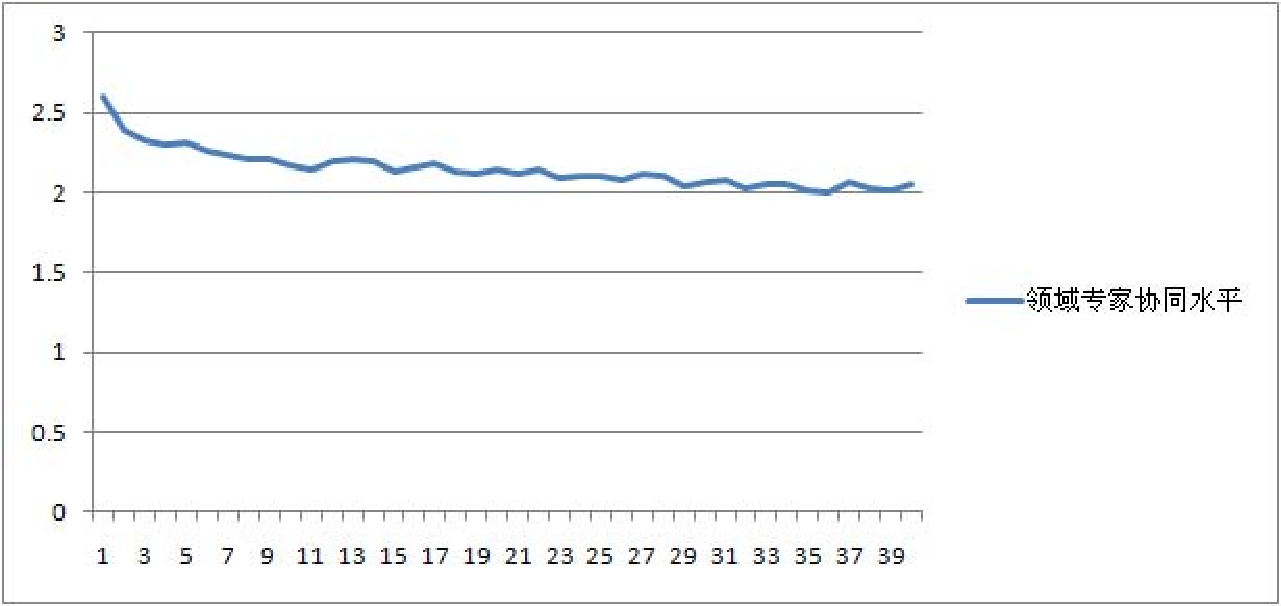
\includegraphics{improve4.pdf}}
  % GNUPLOT: LaTeX picture
\setlength{\unitlength}{0.240900pt}
\ifx\plotpoint\undefined\newsavebox{\plotpoint}\fi
\begin{picture}(1500,900)(0,0)
\sbox{\plotpoint}{\rule[-0.200pt]{0.400pt}{0.400pt}}%
\put(131.0,82.0){\rule[-0.200pt]{4.818pt}{0.400pt}}
\put(111,82){\makebox(0,0)[r]{ 0}}
\put(1419.0,82.0){\rule[-0.200pt]{4.818pt}{0.400pt}}
\put(131.0,276.0){\rule[-0.200pt]{4.818pt}{0.400pt}}
\put(111,276){\makebox(0,0)[r]{ 1}}
\put(1419.0,276.0){\rule[-0.200pt]{4.818pt}{0.400pt}}
\put(131.0,471.0){\rule[-0.200pt]{4.818pt}{0.400pt}}
\put(111,471){\makebox(0,0)[r]{ 2}}
\put(1419.0,471.0){\rule[-0.200pt]{4.818pt}{0.400pt}}
\put(131.0,665.0){\rule[-0.200pt]{4.818pt}{0.400pt}}
\put(111,665){\makebox(0,0)[r]{ 3}}
\put(1419.0,665.0){\rule[-0.200pt]{4.818pt}{0.400pt}}
\put(131.0,82.0){\rule[-0.200pt]{0.400pt}{4.818pt}}
\put(131,41){\makebox(0,0){ 1}}
\put(131.0,839.0){\rule[-0.200pt]{0.400pt}{4.818pt}}
\put(198.0,82.0){\rule[-0.200pt]{0.400pt}{4.818pt}}
\put(198,41){\makebox(0,0){ 3}}
\put(198.0,839.0){\rule[-0.200pt]{0.400pt}{4.818pt}}
\put(265.0,82.0){\rule[-0.200pt]{0.400pt}{4.818pt}}
\put(265,41){\makebox(0,0){ 5}}
\put(265.0,839.0){\rule[-0.200pt]{0.400pt}{4.818pt}}
\put(332.0,82.0){\rule[-0.200pt]{0.400pt}{4.818pt}}
\put(332,41){\makebox(0,0){ 7}}
\put(332.0,839.0){\rule[-0.200pt]{0.400pt}{4.818pt}}
\put(399.0,82.0){\rule[-0.200pt]{0.400pt}{4.818pt}}
\put(399,41){\makebox(0,0){ 9}}
\put(399.0,839.0){\rule[-0.200pt]{0.400pt}{4.818pt}}
\put(466.0,82.0){\rule[-0.200pt]{0.400pt}{4.818pt}}
\put(466,41){\makebox(0,0){ 11}}
\put(466.0,839.0){\rule[-0.200pt]{0.400pt}{4.818pt}}
\put(533.0,82.0){\rule[-0.200pt]{0.400pt}{4.818pt}}
\put(533,41){\makebox(0,0){ 13}}
\put(533.0,839.0){\rule[-0.200pt]{0.400pt}{4.818pt}}
\put(601.0,82.0){\rule[-0.200pt]{0.400pt}{4.818pt}}
\put(601,41){\makebox(0,0){ 15}}
\put(601.0,839.0){\rule[-0.200pt]{0.400pt}{4.818pt}}
\put(668.0,82.0){\rule[-0.200pt]{0.400pt}{4.818pt}}
\put(668,41){\makebox(0,0){ 17}}
\put(668.0,839.0){\rule[-0.200pt]{0.400pt}{4.818pt}}
\put(735.0,82.0){\rule[-0.200pt]{0.400pt}{4.818pt}}
\put(735,41){\makebox(0,0){ 19}}
\put(735.0,839.0){\rule[-0.200pt]{0.400pt}{4.818pt}}
\put(802.0,82.0){\rule[-0.200pt]{0.400pt}{4.818pt}}
\put(802,41){\makebox(0,0){ 21}}
\put(802.0,839.0){\rule[-0.200pt]{0.400pt}{4.818pt}}
\put(869.0,82.0){\rule[-0.200pt]{0.400pt}{4.818pt}}
\put(869,41){\makebox(0,0){ 23}}
\put(869.0,839.0){\rule[-0.200pt]{0.400pt}{4.818pt}}
\put(936.0,82.0){\rule[-0.200pt]{0.400pt}{4.818pt}}
\put(936,41){\makebox(0,0){ 25}}
\put(936.0,839.0){\rule[-0.200pt]{0.400pt}{4.818pt}}
\put(1003.0,82.0){\rule[-0.200pt]{0.400pt}{4.818pt}}
\put(1003,41){\makebox(0,0){ 27}}
\put(1003.0,839.0){\rule[-0.200pt]{0.400pt}{4.818pt}}
\put(1070.0,82.0){\rule[-0.200pt]{0.400pt}{4.818pt}}
\put(1070,41){\makebox(0,0){ 29}}
\put(1070.0,839.0){\rule[-0.200pt]{0.400pt}{4.818pt}}
\put(1137.0,82.0){\rule[-0.200pt]{0.400pt}{4.818pt}}
\put(1137,41){\makebox(0,0){ 31}}
\put(1137.0,839.0){\rule[-0.200pt]{0.400pt}{4.818pt}}
\put(1204.0,82.0){\rule[-0.200pt]{0.400pt}{4.818pt}}
\put(1204,41){\makebox(0,0){ 33}}
\put(1204.0,839.0){\rule[-0.200pt]{0.400pt}{4.818pt}}
\put(1271.0,82.0){\rule[-0.200pt]{0.400pt}{4.818pt}}
\put(1271,41){\makebox(0,0){ 35}}
\put(1271.0,839.0){\rule[-0.200pt]{0.400pt}{4.818pt}}
\put(1338.0,82.0){\rule[-0.200pt]{0.400pt}{4.818pt}}
\put(1338,41){\makebox(0,0){ 37}}
\put(1338.0,839.0){\rule[-0.200pt]{0.400pt}{4.818pt}}
\put(1405.0,82.0){\rule[-0.200pt]{0.400pt}{4.818pt}}
\put(1405,41){\makebox(0,0){ 39}}
\put(1405.0,839.0){\rule[-0.200pt]{0.400pt}{4.818pt}}
\put(131.0,82.0){\rule[-0.200pt]{0.400pt}{187.179pt}}
\put(131.0,82.0){\rule[-0.200pt]{315.097pt}{0.400pt}}
\put(1439.0,82.0){\rule[-0.200pt]{0.400pt}{187.179pt}}
\put(131.0,859.0){\rule[-0.200pt]{315.097pt}{0.400pt}}
\put(30,470){\makebox(0,0){\rotatebox{90}{用户贡献}}}
\put(1279,819){\makebox(0,0)[r]{仿真数据}}
\put(1299.0,819.0){\rule[-0.200pt]{24.090pt}{0.400pt}}
\put(131,366){\usebox{\plotpoint}}
\multiput(131.00,364.92)(0.952,-0.495){33}{\rule{0.856pt}{0.119pt}}
\multiput(131.00,365.17)(32.224,-18.000){2}{\rule{0.428pt}{0.400pt}}
\multiput(165.00,346.92)(1.401,-0.492){21}{\rule{1.200pt}{0.119pt}}
\multiput(165.00,347.17)(30.509,-12.000){2}{\rule{0.600pt}{0.400pt}}
\multiput(198.00,334.93)(3.716,-0.477){7}{\rule{2.820pt}{0.115pt}}
\multiput(198.00,335.17)(28.147,-5.000){2}{\rule{1.410pt}{0.400pt}}
\multiput(232.00,329.93)(2.932,-0.482){9}{\rule{2.300pt}{0.116pt}}
\multiput(232.00,330.17)(28.226,-6.000){2}{\rule{1.150pt}{0.400pt}}
\multiput(265.00,323.93)(3.022,-0.482){9}{\rule{2.367pt}{0.116pt}}
\multiput(265.00,324.17)(29.088,-6.000){2}{\rule{1.183pt}{0.400pt}}
\multiput(299.00,317.94)(4.722,-0.468){5}{\rule{3.400pt}{0.113pt}}
\multiput(299.00,318.17)(25.943,-4.000){2}{\rule{1.700pt}{0.400pt}}
\put(332,313.17){\rule{6.900pt}{0.400pt}}
\multiput(332.00,314.17)(19.679,-2.000){2}{\rule{3.450pt}{0.400pt}}
\multiput(366.00,311.94)(4.722,-0.468){5}{\rule{3.400pt}{0.113pt}}
\multiput(366.00,312.17)(25.943,-4.000){2}{\rule{1.700pt}{0.400pt}}
\put(399,307.17){\rule{6.900pt}{0.400pt}}
\multiput(399.00,308.17)(19.679,-2.000){2}{\rule{3.450pt}{0.400pt}}
\put(433,305.17){\rule{6.700pt}{0.400pt}}
\multiput(433.00,306.17)(19.094,-2.000){2}{\rule{3.350pt}{0.400pt}}
\put(466,303.17){\rule{6.900pt}{0.400pt}}
\multiput(466.00,304.17)(19.679,-2.000){2}{\rule{3.450pt}{0.400pt}}
\put(500,301.67){\rule{7.950pt}{0.400pt}}
\multiput(500.00,302.17)(16.500,-1.000){2}{\rule{3.975pt}{0.400pt}}
\put(533,300.17){\rule{6.900pt}{0.400pt}}
\multiput(533.00,301.17)(19.679,-2.000){2}{\rule{3.450pt}{0.400pt}}
\put(567,298.17){\rule{6.900pt}{0.400pt}}
\multiput(567.00,299.17)(19.679,-2.000){2}{\rule{3.450pt}{0.400pt}}
\put(601,296.17){\rule{6.700pt}{0.400pt}}
\multiput(601.00,297.17)(19.094,-2.000){2}{\rule{3.350pt}{0.400pt}}
\put(634,294.17){\rule{6.900pt}{0.400pt}}
\multiput(634.00,295.17)(19.679,-2.000){2}{\rule{3.450pt}{0.400pt}}
\put(668,292.17){\rule{6.700pt}{0.400pt}}
\multiput(668.00,293.17)(19.094,-2.000){2}{\rule{3.350pt}{0.400pt}}
\put(735,290.17){\rule{6.700pt}{0.400pt}}
\multiput(735.00,291.17)(19.094,-2.000){2}{\rule{3.350pt}{0.400pt}}
\put(768,288.17){\rule{6.900pt}{0.400pt}}
\multiput(768.00,289.17)(19.679,-2.000){2}{\rule{3.450pt}{0.400pt}}
\put(701.0,292.0){\rule[-0.200pt]{8.191pt}{0.400pt}}
\put(835,286.17){\rule{6.900pt}{0.400pt}}
\multiput(835.00,287.17)(19.679,-2.000){2}{\rule{3.450pt}{0.400pt}}
\put(802.0,288.0){\rule[-0.200pt]{7.950pt}{0.400pt}}
\put(902,284.17){\rule{6.900pt}{0.400pt}}
\multiput(902.00,285.17)(19.679,-2.000){2}{\rule{3.450pt}{0.400pt}}
\put(869.0,286.0){\rule[-0.200pt]{7.950pt}{0.400pt}}
\put(969,282.17){\rule{6.900pt}{0.400pt}}
\multiput(969.00,283.17)(19.679,-2.000){2}{\rule{3.450pt}{0.400pt}}
\put(936.0,284.0){\rule[-0.200pt]{7.950pt}{0.400pt}}
\put(1037,280.17){\rule{6.700pt}{0.400pt}}
\multiput(1037.00,281.17)(19.094,-2.000){2}{\rule{3.350pt}{0.400pt}}
\put(1003.0,282.0){\rule[-0.200pt]{8.191pt}{0.400pt}}
\put(1104,278.17){\rule{6.700pt}{0.400pt}}
\multiput(1104.00,279.17)(19.094,-2.000){2}{\rule{3.350pt}{0.400pt}}
\put(1070.0,280.0){\rule[-0.200pt]{8.191pt}{0.400pt}}
\put(1171,276.17){\rule{6.700pt}{0.400pt}}
\multiput(1171.00,277.17)(19.094,-2.000){2}{\rule{3.350pt}{0.400pt}}
\put(1137.0,278.0){\rule[-0.200pt]{8.191pt}{0.400pt}}
\put(1271,274.17){\rule{6.900pt}{0.400pt}}
\multiput(1271.00,275.17)(19.679,-2.000){2}{\rule{3.450pt}{0.400pt}}
\put(1204.0,276.0){\rule[-0.200pt]{16.140pt}{0.400pt}}
\put(1372,272.17){\rule{6.700pt}{0.400pt}}
\multiput(1372.00,273.17)(19.094,-2.000){2}{\rule{3.350pt}{0.400pt}}
\put(1305.0,274.0){\rule[-0.200pt]{16.140pt}{0.400pt}}
\put(1405.0,272.0){\rule[-0.200pt]{8.191pt}{0.400pt}}
\put(1279,768){\makebox(0,0)[r]{改进数据}}
\put(1299.0,768.0){\rule[-0.200pt]{24.090pt}{0.400pt}}
\put(131,587){\usebox{\plotpoint}}
\multiput(131.00,585.92)(0.514,-0.497){63}{\rule{0.512pt}{0.120pt}}
\multiput(131.00,586.17)(32.937,-33.000){2}{\rule{0.256pt}{0.400pt}}
\multiput(165.00,552.93)(2.145,-0.488){13}{\rule{1.750pt}{0.117pt}}
\multiput(165.00,553.17)(29.368,-8.000){2}{\rule{0.875pt}{0.400pt}}
\multiput(198.00,544.92)(1.581,-0.492){19}{\rule{1.336pt}{0.118pt}}
\multiput(198.00,545.17)(31.226,-11.000){2}{\rule{0.668pt}{0.400pt}}
\multiput(232.00,533.93)(2.145,-0.488){13}{\rule{1.750pt}{0.117pt}}
\multiput(232.00,534.17)(29.368,-8.000){2}{\rule{0.875pt}{0.400pt}}
\put(265,527.17){\rule{6.900pt}{0.400pt}}
\multiput(265.00,526.17)(19.679,2.000){2}{\rule{3.450pt}{0.400pt}}
\multiput(299.00,527.93)(2.932,-0.482){9}{\rule{2.300pt}{0.116pt}}
\multiput(299.00,528.17)(28.226,-6.000){2}{\rule{1.150pt}{0.400pt}}
\put(332,523.17){\rule{6.900pt}{0.400pt}}
\multiput(332.00,522.17)(19.679,2.000){2}{\rule{3.450pt}{0.400pt}}
\multiput(366.00,523.92)(1.694,-0.491){17}{\rule{1.420pt}{0.118pt}}
\multiput(366.00,524.17)(30.053,-10.000){2}{\rule{0.710pt}{0.400pt}}
\put(399,515.17){\rule{6.900pt}{0.400pt}}
\multiput(399.00,514.17)(19.679,2.000){2}{\rule{3.450pt}{0.400pt}}
\multiput(433.00,515.93)(2.145,-0.488){13}{\rule{1.750pt}{0.117pt}}
\multiput(433.00,516.17)(29.368,-8.000){2}{\rule{0.875pt}{0.400pt}}
\put(466,507.17){\rule{6.900pt}{0.400pt}}
\multiput(466.00,508.17)(19.679,-2.000){2}{\rule{3.450pt}{0.400pt}}
\multiput(500.00,507.60)(4.722,0.468){5}{\rule{3.400pt}{0.113pt}}
\multiput(500.00,506.17)(25.943,4.000){2}{\rule{1.700pt}{0.400pt}}
\put(533,509.17){\rule{6.900pt}{0.400pt}}
\multiput(533.00,510.17)(19.679,-2.000){2}{\rule{3.450pt}{0.400pt}}
\multiput(567.00,507.94)(4.868,-0.468){5}{\rule{3.500pt}{0.113pt}}
\multiput(567.00,508.17)(26.736,-4.000){2}{\rule{1.750pt}{0.400pt}}
\multiput(601.00,503.95)(7.160,-0.447){3}{\rule{4.500pt}{0.108pt}}
\multiput(601.00,504.17)(23.660,-3.000){2}{\rule{2.250pt}{0.400pt}}
\put(634,500.17){\rule{6.900pt}{0.400pt}}
\multiput(634.00,501.17)(19.679,-2.000){2}{\rule{3.450pt}{0.400pt}}
\multiput(668.00,500.60)(4.722,0.468){5}{\rule{3.400pt}{0.113pt}}
\multiput(668.00,499.17)(25.943,4.000){2}{\rule{1.700pt}{0.400pt}}
\multiput(701.00,502.94)(4.868,-0.468){5}{\rule{3.500pt}{0.113pt}}
\multiput(701.00,503.17)(26.736,-4.000){2}{\rule{1.750pt}{0.400pt}}
\multiput(735.00,500.60)(4.722,0.468){5}{\rule{3.400pt}{0.113pt}}
\multiput(735.00,499.17)(25.943,4.000){2}{\rule{1.700pt}{0.400pt}}
\multiput(768.00,502.93)(2.211,-0.488){13}{\rule{1.800pt}{0.117pt}}
\multiput(768.00,503.17)(30.264,-8.000){2}{\rule{0.900pt}{0.400pt}}
\put(802,494.17){\rule{6.700pt}{0.400pt}}
\multiput(802.00,495.17)(19.094,-2.000){2}{\rule{3.350pt}{0.400pt}}
\multiput(835.00,492.93)(3.022,-0.482){9}{\rule{2.367pt}{0.116pt}}
\multiput(835.00,493.17)(29.088,-6.000){2}{\rule{1.183pt}{0.400pt}}
\multiput(869.00,488.59)(2.932,0.482){9}{\rule{2.300pt}{0.116pt}}
\multiput(869.00,487.17)(28.226,6.000){2}{\rule{1.150pt}{0.400pt}}
\put(902,492.17){\rule{6.900pt}{0.400pt}}
\multiput(902.00,493.17)(19.679,-2.000){2}{\rule{3.450pt}{0.400pt}}
\multiput(969.00,490.94)(4.868,-0.468){5}{\rule{3.500pt}{0.113pt}}
\multiput(969.00,491.17)(26.736,-4.000){2}{\rule{1.750pt}{0.400pt}}
\put(1003,488.17){\rule{6.900pt}{0.400pt}}
\multiput(1003.00,487.17)(19.679,2.000){2}{\rule{3.450pt}{0.400pt}}
\multiput(1037.00,490.60)(4.722,0.468){5}{\rule{3.400pt}{0.113pt}}
\multiput(1037.00,489.17)(25.943,4.000){2}{\rule{1.700pt}{0.400pt}}
\multiput(1070.00,492.93)(2.211,-0.488){13}{\rule{1.800pt}{0.117pt}}
\multiput(1070.00,493.17)(30.264,-8.000){2}{\rule{0.900pt}{0.400pt}}
\multiput(1104.00,484.93)(2.932,-0.482){9}{\rule{2.300pt}{0.116pt}}
\multiput(1104.00,485.17)(28.226,-6.000){2}{\rule{1.150pt}{0.400pt}}
\put(1137,478.17){\rule{6.900pt}{0.400pt}}
\multiput(1137.00,479.17)(19.679,-2.000){2}{\rule{3.450pt}{0.400pt}}
\put(1171,476.17){\rule{6.700pt}{0.400pt}}
\multiput(1171.00,477.17)(19.094,-2.000){2}{\rule{3.350pt}{0.400pt}}
\multiput(1204.00,476.59)(2.211,0.488){13}{\rule{1.800pt}{0.117pt}}
\multiput(1204.00,475.17)(30.264,8.000){2}{\rule{0.900pt}{0.400pt}}
\multiput(1238.00,482.92)(1.694,-0.491){17}{\rule{1.420pt}{0.118pt}}
\multiput(1238.00,483.17)(30.053,-10.000){2}{\rule{0.710pt}{0.400pt}}
\put(1271,472.17){\rule{6.900pt}{0.400pt}}
\multiput(1271.00,473.17)(19.679,-2.000){2}{\rule{3.450pt}{0.400pt}}
\multiput(1305.00,472.58)(1.694,0.491){17}{\rule{1.420pt}{0.118pt}}
\multiput(1305.00,471.17)(30.053,10.000){2}{\rule{0.710pt}{0.400pt}}
\multiput(1338.00,480.92)(1.581,-0.492){19}{\rule{1.336pt}{0.118pt}}
\multiput(1338.00,481.17)(31.226,-11.000){2}{\rule{0.668pt}{0.400pt}}
\multiput(1372.00,471.59)(3.604,0.477){7}{\rule{2.740pt}{0.115pt}}
\multiput(1372.00,470.17)(27.313,5.000){2}{\rule{1.370pt}{0.400pt}}
\multiput(1405.00,476.59)(3.022,0.482){9}{\rule{2.367pt}{0.116pt}}
\multiput(1405.00,475.17)(29.088,6.000){2}{\rule{1.183pt}{0.400pt}}
\put(131,587){\makebox(0,0){$+$}}
\put(165,554){\makebox(0,0){$+$}}
\put(198,546){\makebox(0,0){$+$}}
\put(232,535){\makebox(0,0){$+$}}
\put(265,527){\makebox(0,0){$+$}}
\put(299,529){\makebox(0,0){$+$}}
\put(332,523){\makebox(0,0){$+$}}
\put(366,525){\makebox(0,0){$+$}}
\put(399,515){\makebox(0,0){$+$}}
\put(433,517){\makebox(0,0){$+$}}
\put(466,509){\makebox(0,0){$+$}}
\put(500,507){\makebox(0,0){$+$}}
\put(533,511){\makebox(0,0){$+$}}
\put(567,509){\makebox(0,0){$+$}}
\put(601,505){\makebox(0,0){$+$}}
\put(634,502){\makebox(0,0){$+$}}
\put(668,500){\makebox(0,0){$+$}}
\put(701,504){\makebox(0,0){$+$}}
\put(735,500){\makebox(0,0){$+$}}
\put(768,504){\makebox(0,0){$+$}}
\put(802,496){\makebox(0,0){$+$}}
\put(835,494){\makebox(0,0){$+$}}
\put(869,488){\makebox(0,0){$+$}}
\put(902,494){\makebox(0,0){$+$}}
\put(936,492){\makebox(0,0){$+$}}
\put(969,492){\makebox(0,0){$+$}}
\put(1003,488){\makebox(0,0){$+$}}
\put(1037,490){\makebox(0,0){$+$}}
\put(1070,494){\makebox(0,0){$+$}}
\put(1104,486){\makebox(0,0){$+$}}
\put(1137,480){\makebox(0,0){$+$}}
\put(1171,478){\makebox(0,0){$+$}}
\put(1204,476){\makebox(0,0){$+$}}
\put(1238,484){\makebox(0,0){$+$}}
\put(1271,474){\makebox(0,0){$+$}}
\put(1305,472){\makebox(0,0){$+$}}
\put(1338,482){\makebox(0,0){$+$}}
\put(1372,471){\makebox(0,0){$+$}}
\put(1405,476){\makebox(0,0){$+$}}
\put(1439,482){\makebox(0,0){$+$}}
\put(1349,768){\makebox(0,0){$+$}}
\put(936.0,492.0){\rule[-0.200pt]{7.950pt}{0.400pt}}
\put(131.0,82.0){\rule[-0.200pt]{0.400pt}{187.179pt}}
\put(131.0,82.0){\rule[-0.200pt]{315.097pt}{0.400pt}}
\put(1439.0,82.0){\rule[-0.200pt]{0.400pt}{187.179pt}}
\put(131.0,859.0){\rule[-0.200pt]{315.097pt}{0.400pt}}
\end{picture}
 
 \caption{\small{\textbf{提升领域专家所有动机的仿真结果}}}
  \label{fig:improve4}
\end{figure}

%图是领域专家用户和领导者成就感变量的仿真结果。可以看到领域专家的成就
%感一直处在非常高的位置,而领导者的成就感则稳定在一个很低的水平。
图\ref{fig:improve3}是将领域专家用户除了成就需求以外的其他动机因素提升$10\%$
的结果。提升后贡献值的趋势发生了较大的变化,不在是逐步下降,而是稳步上
升。这两个仿真结果揭示了两类用户的根本差异。领域专家用户的成就需求在所
有动机中占了较大的比重,也就说领域专家用户相对来说更注重成就的取得。但
是,该类用户的成就感消失的很慢,他们在协同过程中迅速满足了自身的成就需
求,并且一直在享受所取得的成就。相比之下,领导者用户的成就感很快消失,
能使其一直保持参与知识协同的动力。

\begin{figure}[!htb]
  \centering
%  \scalebox{0.65}{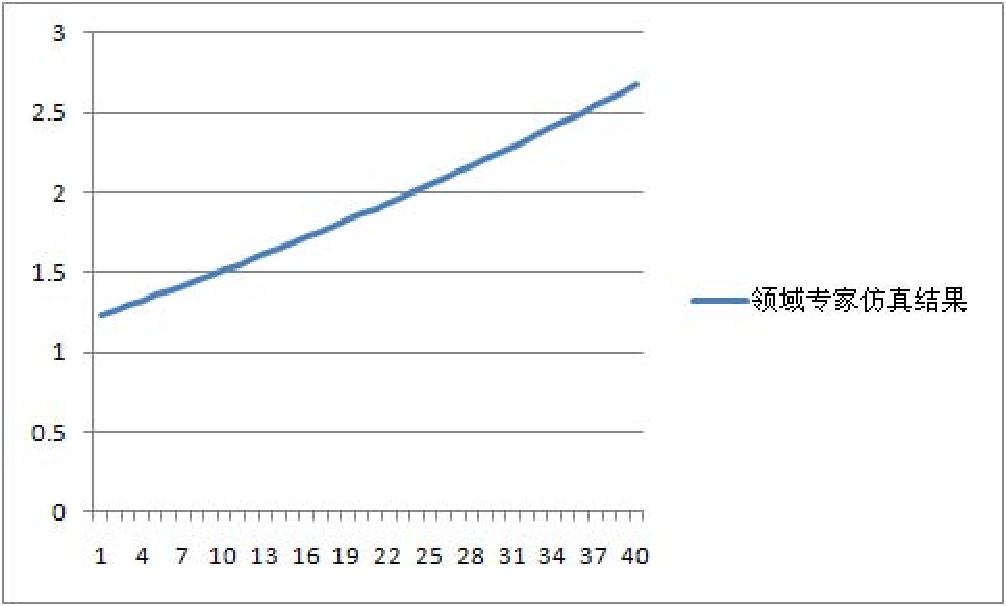
\includegraphics{improve3.pdf}}
  \caption{\small{\textbf{提升领域专家成就动机的仿真结果}}}
  % GNUPLOT: LaTeX picture
\setlength{\unitlength}{0.240900pt}
\ifx\plotpoint\undefined\newsavebox{\plotpoint}\fi
\begin{picture}(1500,900)(0,0)
\sbox{\plotpoint}{\rule[-0.200pt]{0.400pt}{0.400pt}}%
\put(131.0,82.0){\rule[-0.200pt]{4.818pt}{0.400pt}}
\put(111,82){\makebox(0,0)[r]{ 0}}
\put(1419.0,82.0){\rule[-0.200pt]{4.818pt}{0.400pt}}
\put(131.0,276.0){\rule[-0.200pt]{4.818pt}{0.400pt}}
\put(111,276){\makebox(0,0)[r]{ 1}}
\put(1419.0,276.0){\rule[-0.200pt]{4.818pt}{0.400pt}}
\put(131.0,471.0){\rule[-0.200pt]{4.818pt}{0.400pt}}
\put(111,471){\makebox(0,0)[r]{ 2}}
\put(1419.0,471.0){\rule[-0.200pt]{4.818pt}{0.400pt}}
\put(131.0,665.0){\rule[-0.200pt]{4.818pt}{0.400pt}}
\put(111,665){\makebox(0,0)[r]{ 3}}
\put(1419.0,665.0){\rule[-0.200pt]{4.818pt}{0.400pt}}
\put(131.0,82.0){\rule[-0.200pt]{0.400pt}{4.818pt}}
\put(131,41){\makebox(0,0){ 1}}
\put(131.0,839.0){\rule[-0.200pt]{0.400pt}{4.818pt}}
\put(198.0,82.0){\rule[-0.200pt]{0.400pt}{4.818pt}}
\put(198,41){\makebox(0,0){ 3}}
\put(198.0,839.0){\rule[-0.200pt]{0.400pt}{4.818pt}}
\put(265.0,82.0){\rule[-0.200pt]{0.400pt}{4.818pt}}
\put(265,41){\makebox(0,0){ 5}}
\put(265.0,839.0){\rule[-0.200pt]{0.400pt}{4.818pt}}
\put(332.0,82.0){\rule[-0.200pt]{0.400pt}{4.818pt}}
\put(332,41){\makebox(0,0){ 7}}
\put(332.0,839.0){\rule[-0.200pt]{0.400pt}{4.818pt}}
\put(399.0,82.0){\rule[-0.200pt]{0.400pt}{4.818pt}}
\put(399,41){\makebox(0,0){ 9}}
\put(399.0,839.0){\rule[-0.200pt]{0.400pt}{4.818pt}}
\put(466.0,82.0){\rule[-0.200pt]{0.400pt}{4.818pt}}
\put(466,41){\makebox(0,0){ 11}}
\put(466.0,839.0){\rule[-0.200pt]{0.400pt}{4.818pt}}
\put(533.0,82.0){\rule[-0.200pt]{0.400pt}{4.818pt}}
\put(533,41){\makebox(0,0){ 13}}
\put(533.0,839.0){\rule[-0.200pt]{0.400pt}{4.818pt}}
\put(601.0,82.0){\rule[-0.200pt]{0.400pt}{4.818pt}}
\put(601,41){\makebox(0,0){ 15}}
\put(601.0,839.0){\rule[-0.200pt]{0.400pt}{4.818pt}}
\put(668.0,82.0){\rule[-0.200pt]{0.400pt}{4.818pt}}
\put(668,41){\makebox(0,0){ 17}}
\put(668.0,839.0){\rule[-0.200pt]{0.400pt}{4.818pt}}
\put(735.0,82.0){\rule[-0.200pt]{0.400pt}{4.818pt}}
\put(735,41){\makebox(0,0){ 19}}
\put(735.0,839.0){\rule[-0.200pt]{0.400pt}{4.818pt}}
\put(802.0,82.0){\rule[-0.200pt]{0.400pt}{4.818pt}}
\put(802,41){\makebox(0,0){ 21}}
\put(802.0,839.0){\rule[-0.200pt]{0.400pt}{4.818pt}}
\put(869.0,82.0){\rule[-0.200pt]{0.400pt}{4.818pt}}
\put(869,41){\makebox(0,0){ 23}}
\put(869.0,839.0){\rule[-0.200pt]{0.400pt}{4.818pt}}
\put(936.0,82.0){\rule[-0.200pt]{0.400pt}{4.818pt}}
\put(936,41){\makebox(0,0){ 25}}
\put(936.0,839.0){\rule[-0.200pt]{0.400pt}{4.818pt}}
\put(1003.0,82.0){\rule[-0.200pt]{0.400pt}{4.818pt}}
\put(1003,41){\makebox(0,0){ 27}}
\put(1003.0,839.0){\rule[-0.200pt]{0.400pt}{4.818pt}}
\put(1070.0,82.0){\rule[-0.200pt]{0.400pt}{4.818pt}}
\put(1070,41){\makebox(0,0){ 29}}
\put(1070.0,839.0){\rule[-0.200pt]{0.400pt}{4.818pt}}
\put(1137.0,82.0){\rule[-0.200pt]{0.400pt}{4.818pt}}
\put(1137,41){\makebox(0,0){ 31}}
\put(1137.0,839.0){\rule[-0.200pt]{0.400pt}{4.818pt}}
\put(1204.0,82.0){\rule[-0.200pt]{0.400pt}{4.818pt}}
\put(1204,41){\makebox(0,0){ 33}}
\put(1204.0,839.0){\rule[-0.200pt]{0.400pt}{4.818pt}}
\put(1271.0,82.0){\rule[-0.200pt]{0.400pt}{4.818pt}}
\put(1271,41){\makebox(0,0){ 35}}
\put(1271.0,839.0){\rule[-0.200pt]{0.400pt}{4.818pt}}
\put(1338.0,82.0){\rule[-0.200pt]{0.400pt}{4.818pt}}
\put(1338,41){\makebox(0,0){ 37}}
\put(1338.0,839.0){\rule[-0.200pt]{0.400pt}{4.818pt}}
\put(1405.0,82.0){\rule[-0.200pt]{0.400pt}{4.818pt}}
\put(1405,41){\makebox(0,0){ 39}}
\put(1405.0,839.0){\rule[-0.200pt]{0.400pt}{4.818pt}}
\put(131.0,82.0){\rule[-0.200pt]{0.400pt}{187.179pt}}
\put(131.0,82.0){\rule[-0.200pt]{315.097pt}{0.400pt}}
\put(1439.0,82.0){\rule[-0.200pt]{0.400pt}{187.179pt}}
\put(131.0,859.0){\rule[-0.200pt]{315.097pt}{0.400pt}}
\put(30,470){\makebox(0,0){\rotatebox{90}{用户贡献}}}
\put(1279,819){\makebox(0,0)[r]{仿真数据}}
\put(1299.0,819.0){\rule[-0.200pt]{24.090pt}{0.400pt}}
\put(131,366){\usebox{\plotpoint}}
\multiput(131.00,364.92)(0.952,-0.495){33}{\rule{0.856pt}{0.119pt}}
\multiput(131.00,365.17)(32.224,-18.000){2}{\rule{0.428pt}{0.400pt}}
\multiput(165.00,346.92)(1.401,-0.492){21}{\rule{1.200pt}{0.119pt}}
\multiput(165.00,347.17)(30.509,-12.000){2}{\rule{0.600pt}{0.400pt}}
\multiput(198.00,334.93)(3.716,-0.477){7}{\rule{2.820pt}{0.115pt}}
\multiput(198.00,335.17)(28.147,-5.000){2}{\rule{1.410pt}{0.400pt}}
\multiput(232.00,329.93)(2.932,-0.482){9}{\rule{2.300pt}{0.116pt}}
\multiput(232.00,330.17)(28.226,-6.000){2}{\rule{1.150pt}{0.400pt}}
\multiput(265.00,323.93)(3.022,-0.482){9}{\rule{2.367pt}{0.116pt}}
\multiput(265.00,324.17)(29.088,-6.000){2}{\rule{1.183pt}{0.400pt}}
\multiput(299.00,317.94)(4.722,-0.468){5}{\rule{3.400pt}{0.113pt}}
\multiput(299.00,318.17)(25.943,-4.000){2}{\rule{1.700pt}{0.400pt}}
\put(332,313.17){\rule{6.900pt}{0.400pt}}
\multiput(332.00,314.17)(19.679,-2.000){2}{\rule{3.450pt}{0.400pt}}
\multiput(366.00,311.94)(4.722,-0.468){5}{\rule{3.400pt}{0.113pt}}
\multiput(366.00,312.17)(25.943,-4.000){2}{\rule{1.700pt}{0.400pt}}
\put(399,307.17){\rule{6.900pt}{0.400pt}}
\multiput(399.00,308.17)(19.679,-2.000){2}{\rule{3.450pt}{0.400pt}}
\put(433,305.17){\rule{6.700pt}{0.400pt}}
\multiput(433.00,306.17)(19.094,-2.000){2}{\rule{3.350pt}{0.400pt}}
\put(466,303.17){\rule{6.900pt}{0.400pt}}
\multiput(466.00,304.17)(19.679,-2.000){2}{\rule{3.450pt}{0.400pt}}
\put(500,301.67){\rule{7.950pt}{0.400pt}}
\multiput(500.00,302.17)(16.500,-1.000){2}{\rule{3.975pt}{0.400pt}}
\put(533,300.17){\rule{6.900pt}{0.400pt}}
\multiput(533.00,301.17)(19.679,-2.000){2}{\rule{3.450pt}{0.400pt}}
\put(567,298.17){\rule{6.900pt}{0.400pt}}
\multiput(567.00,299.17)(19.679,-2.000){2}{\rule{3.450pt}{0.400pt}}
\put(601,296.17){\rule{6.700pt}{0.400pt}}
\multiput(601.00,297.17)(19.094,-2.000){2}{\rule{3.350pt}{0.400pt}}
\put(634,294.17){\rule{6.900pt}{0.400pt}}
\multiput(634.00,295.17)(19.679,-2.000){2}{\rule{3.450pt}{0.400pt}}
\put(668,292.17){\rule{6.700pt}{0.400pt}}
\multiput(668.00,293.17)(19.094,-2.000){2}{\rule{3.350pt}{0.400pt}}
\put(735,290.17){\rule{6.700pt}{0.400pt}}
\multiput(735.00,291.17)(19.094,-2.000){2}{\rule{3.350pt}{0.400pt}}
\put(768,288.17){\rule{6.900pt}{0.400pt}}
\multiput(768.00,289.17)(19.679,-2.000){2}{\rule{3.450pt}{0.400pt}}
\put(701.0,292.0){\rule[-0.200pt]{8.191pt}{0.400pt}}
\put(835,286.17){\rule{6.900pt}{0.400pt}}
\multiput(835.00,287.17)(19.679,-2.000){2}{\rule{3.450pt}{0.400pt}}
\put(802.0,288.0){\rule[-0.200pt]{7.950pt}{0.400pt}}
\put(902,284.17){\rule{6.900pt}{0.400pt}}
\multiput(902.00,285.17)(19.679,-2.000){2}{\rule{3.450pt}{0.400pt}}
\put(869.0,286.0){\rule[-0.200pt]{7.950pt}{0.400pt}}
\put(969,282.17){\rule{6.900pt}{0.400pt}}
\multiput(969.00,283.17)(19.679,-2.000){2}{\rule{3.450pt}{0.400pt}}
\put(936.0,284.0){\rule[-0.200pt]{7.950pt}{0.400pt}}
\put(1037,280.17){\rule{6.700pt}{0.400pt}}
\multiput(1037.00,281.17)(19.094,-2.000){2}{\rule{3.350pt}{0.400pt}}
\put(1003.0,282.0){\rule[-0.200pt]{8.191pt}{0.400pt}}
\put(1104,278.17){\rule{6.700pt}{0.400pt}}
\multiput(1104.00,279.17)(19.094,-2.000){2}{\rule{3.350pt}{0.400pt}}
\put(1070.0,280.0){\rule[-0.200pt]{8.191pt}{0.400pt}}
\put(1171,276.17){\rule{6.700pt}{0.400pt}}
\multiput(1171.00,277.17)(19.094,-2.000){2}{\rule{3.350pt}{0.400pt}}
\put(1137.0,278.0){\rule[-0.200pt]{8.191pt}{0.400pt}}
\put(1271,274.17){\rule{6.900pt}{0.400pt}}
\multiput(1271.00,275.17)(19.679,-2.000){2}{\rule{3.450pt}{0.400pt}}
\put(1204.0,276.0){\rule[-0.200pt]{16.140pt}{0.400pt}}
\put(1372,272.17){\rule{6.700pt}{0.400pt}}
\multiput(1372.00,273.17)(19.094,-2.000){2}{\rule{3.350pt}{0.400pt}}
\put(1305.0,274.0){\rule[-0.200pt]{16.140pt}{0.400pt}}
\put(1405.0,272.0){\rule[-0.200pt]{8.191pt}{0.400pt}}
\put(1279,768){\makebox(0,0)[r]{改进数据}}
\put(1299.0,768.0){\rule[-0.200pt]{24.090pt}{0.400pt}}
\put(131,379){\usebox{\plotpoint}}
\multiput(131.00,379.59)(3.022,0.482){9}{\rule{2.367pt}{0.116pt}}
\multiput(131.00,378.17)(29.088,6.000){2}{\rule{1.183pt}{0.400pt}}
\multiput(165.00,385.59)(2.932,0.482){9}{\rule{2.300pt}{0.116pt}}
\multiput(165.00,384.17)(28.226,6.000){2}{\rule{1.150pt}{0.400pt}}
\multiput(198.00,391.59)(3.022,0.482){9}{\rule{2.367pt}{0.116pt}}
\multiput(198.00,390.17)(29.088,6.000){2}{\rule{1.183pt}{0.400pt}}
\multiput(265.00,397.61)(7.383,0.447){3}{\rule{4.633pt}{0.108pt}}
\multiput(265.00,396.17)(24.383,3.000){2}{\rule{2.317pt}{0.400pt}}
\multiput(299.00,400.59)(2.932,0.482){9}{\rule{2.300pt}{0.116pt}}
\multiput(299.00,399.17)(28.226,6.000){2}{\rule{1.150pt}{0.400pt}}
\multiput(332.00,406.59)(2.211,0.488){13}{\rule{1.800pt}{0.117pt}}
\multiput(332.00,405.17)(30.264,8.000){2}{\rule{0.900pt}{0.400pt}}
\multiput(366.00,414.61)(7.160,0.447){3}{\rule{4.500pt}{0.108pt}}
\multiput(366.00,413.17)(23.660,3.000){2}{\rule{2.250pt}{0.400pt}}
\put(399,417.17){\rule{6.900pt}{0.400pt}}
\multiput(399.00,416.17)(19.679,2.000){2}{\rule{3.450pt}{0.400pt}}
\multiput(433.00,419.61)(7.160,0.447){3}{\rule{4.500pt}{0.108pt}}
\multiput(433.00,418.17)(23.660,3.000){2}{\rule{2.250pt}{0.400pt}}
\multiput(466.00,422.59)(3.022,0.482){9}{\rule{2.367pt}{0.116pt}}
\multiput(466.00,421.17)(29.088,6.000){2}{\rule{1.183pt}{0.400pt}}
\put(500,427.67){\rule{7.950pt}{0.400pt}}
\multiput(500.00,427.17)(16.500,1.000){2}{\rule{3.975pt}{0.400pt}}
\multiput(533.00,429.58)(1.329,0.493){23}{\rule{1.146pt}{0.119pt}}
\multiput(533.00,428.17)(31.621,13.000){2}{\rule{0.573pt}{0.400pt}}
\multiput(567.00,442.59)(3.022,0.482){9}{\rule{2.367pt}{0.116pt}}
\multiput(567.00,441.17)(29.088,6.000){2}{\rule{1.183pt}{0.400pt}}
\multiput(601.00,448.59)(2.476,0.485){11}{\rule{1.986pt}{0.117pt}}
\multiput(601.00,447.17)(28.879,7.000){2}{\rule{0.993pt}{0.400pt}}
\multiput(634.00,455.58)(1.009,0.495){31}{\rule{0.900pt}{0.119pt}}
\multiput(634.00,454.17)(32.132,17.000){2}{\rule{0.450pt}{0.400pt}}
\multiput(668.00,472.59)(1.893,0.489){15}{\rule{1.567pt}{0.118pt}}
\multiput(668.00,471.17)(29.748,9.000){2}{\rule{0.783pt}{0.400pt}}
\multiput(701.00,481.58)(1.746,0.491){17}{\rule{1.460pt}{0.118pt}}
\multiput(701.00,480.17)(30.970,10.000){2}{\rule{0.730pt}{0.400pt}}
\multiput(735.00,491.60)(4.722,0.468){5}{\rule{3.400pt}{0.113pt}}
\multiput(735.00,490.17)(25.943,4.000){2}{\rule{1.700pt}{0.400pt}}
\multiput(768.00,495.61)(7.383,0.447){3}{\rule{4.633pt}{0.108pt}}
\multiput(768.00,494.17)(24.383,3.000){2}{\rule{2.317pt}{0.400pt}}
\multiput(802.00,498.59)(2.145,0.488){13}{\rule{1.750pt}{0.117pt}}
\multiput(802.00,497.17)(29.368,8.000){2}{\rule{0.875pt}{0.400pt}}
\multiput(835.00,506.59)(2.211,0.488){13}{\rule{1.800pt}{0.117pt}}
\multiput(835.00,505.17)(30.264,8.000){2}{\rule{0.900pt}{0.400pt}}
\multiput(869.00,514.58)(1.041,0.494){29}{\rule{0.925pt}{0.119pt}}
\multiput(869.00,513.17)(31.080,16.000){2}{\rule{0.463pt}{0.400pt}}
\multiput(902.00,530.59)(3.716,0.477){7}{\rule{2.820pt}{0.115pt}}
\multiput(902.00,529.17)(28.147,5.000){2}{\rule{1.410pt}{0.400pt}}
\multiput(936.00,535.59)(2.145,0.488){13}{\rule{1.750pt}{0.117pt}}
\multiput(936.00,534.17)(29.368,8.000){2}{\rule{0.875pt}{0.400pt}}
\multiput(969.00,543.58)(1.581,0.492){19}{\rule{1.336pt}{0.118pt}}
\multiput(969.00,542.17)(31.226,11.000){2}{\rule{0.668pt}{0.400pt}}
\multiput(1003.00,554.59)(2.211,0.488){13}{\rule{1.800pt}{0.117pt}}
\multiput(1003.00,553.17)(30.264,8.000){2}{\rule{0.900pt}{0.400pt}}
\multiput(1037.00,562.59)(2.476,0.485){11}{\rule{1.986pt}{0.117pt}}
\multiput(1037.00,561.17)(28.879,7.000){2}{\rule{0.993pt}{0.400pt}}
\multiput(1070.00,569.59)(2.211,0.488){13}{\rule{1.800pt}{0.117pt}}
\multiput(1070.00,568.17)(30.264,8.000){2}{\rule{0.900pt}{0.400pt}}
\multiput(1104.00,577.59)(2.145,0.488){13}{\rule{1.750pt}{0.117pt}}
\multiput(1104.00,576.17)(29.368,8.000){2}{\rule{0.875pt}{0.400pt}}
\multiput(1137.00,585.59)(2.211,0.488){13}{\rule{1.800pt}{0.117pt}}
\multiput(1137.00,584.17)(30.264,8.000){2}{\rule{0.900pt}{0.400pt}}
\multiput(1171.00,593.59)(2.145,0.488){13}{\rule{1.750pt}{0.117pt}}
\multiput(1171.00,592.17)(29.368,8.000){2}{\rule{0.875pt}{0.400pt}}
\multiput(1204.00,601.59)(2.211,0.488){13}{\rule{1.800pt}{0.117pt}}
\multiput(1204.00,600.17)(30.264,8.000){2}{\rule{0.900pt}{0.400pt}}
\multiput(1238.00,609.59)(1.893,0.489){15}{\rule{1.567pt}{0.118pt}}
\multiput(1238.00,608.17)(29.748,9.000){2}{\rule{0.783pt}{0.400pt}}
\multiput(1271.00,618.59)(2.211,0.488){13}{\rule{1.800pt}{0.117pt}}
\multiput(1271.00,617.17)(30.264,8.000){2}{\rule{0.900pt}{0.400pt}}
\multiput(1305.00,626.59)(2.145,0.488){13}{\rule{1.750pt}{0.117pt}}
\multiput(1305.00,625.17)(29.368,8.000){2}{\rule{0.875pt}{0.400pt}}
\multiput(1338.00,634.59)(1.951,0.489){15}{\rule{1.611pt}{0.118pt}}
\multiput(1338.00,633.17)(30.656,9.000){2}{\rule{0.806pt}{0.400pt}}
\multiput(1372.00,643.59)(2.145,0.488){13}{\rule{1.750pt}{0.117pt}}
\multiput(1372.00,642.17)(29.368,8.000){2}{\rule{0.875pt}{0.400pt}}
\multiput(1405.00,651.59)(1.951,0.489){15}{\rule{1.611pt}{0.118pt}}
\multiput(1405.00,650.17)(30.656,9.000){2}{\rule{0.806pt}{0.400pt}}
\put(131,379){\makebox(0,0){$+$}}
\put(165,385){\makebox(0,0){$+$}}
\put(198,391){\makebox(0,0){$+$}}
\put(232,397){\makebox(0,0){$+$}}
\put(265,397){\makebox(0,0){$+$}}
\put(299,400){\makebox(0,0){$+$}}
\put(332,406){\makebox(0,0){$+$}}
\put(366,414){\makebox(0,0){$+$}}
\put(399,417){\makebox(0,0){$+$}}
\put(433,419){\makebox(0,0){$+$}}
\put(466,422){\makebox(0,0){$+$}}
\put(500,428){\makebox(0,0){$+$}}
\put(533,429){\makebox(0,0){$+$}}
\put(567,442){\makebox(0,0){$+$}}
\put(601,448){\makebox(0,0){$+$}}
\put(634,455){\makebox(0,0){$+$}}
\put(668,472){\makebox(0,0){$+$}}
\put(701,481){\makebox(0,0){$+$}}
\put(735,491){\makebox(0,0){$+$}}
\put(768,495){\makebox(0,0){$+$}}
\put(802,498){\makebox(0,0){$+$}}
\put(835,506){\makebox(0,0){$+$}}
\put(869,514){\makebox(0,0){$+$}}
\put(902,530){\makebox(0,0){$+$}}
\put(936,535){\makebox(0,0){$+$}}
\put(969,543){\makebox(0,0){$+$}}
\put(1003,554){\makebox(0,0){$+$}}
\put(1037,562){\makebox(0,0){$+$}}
\put(1070,569){\makebox(0,0){$+$}}
\put(1104,577){\makebox(0,0){$+$}}
\put(1137,585){\makebox(0,0){$+$}}
\put(1171,593){\makebox(0,0){$+$}}
\put(1204,601){\makebox(0,0){$+$}}
\put(1238,609){\makebox(0,0){$+$}}
\put(1271,618){\makebox(0,0){$+$}}
\put(1305,626){\makebox(0,0){$+$}}
\put(1338,634){\makebox(0,0){$+$}}
\put(1372,643){\makebox(0,0){$+$}}
\put(1405,651){\makebox(0,0){$+$}}
\put(1439,660){\makebox(0,0){$+$}}
\put(1349,768){\makebox(0,0){$+$}}
\put(232.0,397.0){\rule[-0.200pt]{7.950pt}{0.400pt}}
\put(131.0,82.0){\rule[-0.200pt]{0.400pt}{187.179pt}}
\put(131.0,82.0){\rule[-0.200pt]{315.097pt}{0.400pt}}
\put(1439.0,82.0){\rule[-0.200pt]{0.400pt}{187.179pt}}
\put(131.0,859.0){\rule[-0.200pt]{315.097pt}{0.400pt}}
\end{picture}
 
  \label{fig:improve3}
\end{figure}

领域专家用户具有和领导者相似的协同模式和个人能力,但是其容易“自满”的
特点限制了其发挥自身的最大能力。如果社区能够采取措施将领域专家转化为领
导者,那么对于社区的发展将是大有裨益的。首先,应该加强领域专家用户的成
就期待感,让他们认识到仅仅完成一两个条目的撰写还远远不是成功的终点,只
有唤起他们更大的成功欲望,才能有效地克服“自满”情绪。同时,社区给与这
类用户充分的支持和鼓励,这样有助于调整内部动机各个因素间的比率,降低成
就需求的比重,使那些具有正反馈关系的动机占据主要地位,最大限度地提升领
域专家用户的参与水平。

\subsection{内容贡献者}

内容贡献者是社区的中坚力量。个体层面的动机和群体层面的动机都会影响他们
参与知识协同的程度。内容贡献者的月人均贡献度的变化很平缓,但是仍然可以
看到加速上升的趋势,这意味着正反馈对协同水平起到了主要作用。同时,内容
贡献者的贡献度水平非常高,在所有用户群体中仅次于领导者用户。因此,这类
用户并不存在领域专家那种容易“自满”的特点。

尽管内容贡献者的贡献度呈现指数增长的特点,但是其增长速度非常缓慢。通过
对比其月度的总贡献和月度的正贡献可以发现:总贡献和正贡献的值非常接近,
就平均水平而言,正贡献与总贡献的差小于$10\%$,而二者最大的差值仅为
$18\%$。这意味着内容贡献者的工作水平非常高,大部分编辑内容都被其他协同
着接受而得以保留。因此内容贡献者所得到的负反馈实际上是非常少的。造成内
容贡献者贡献增长较慢的主要原因是其动机的初始值较低。只有在经历较长时间
后,正反馈的效应才能逐渐体现出来。内容贡献者同领导者用户不同,他们的动
机水平是在协同过程中不断获得正反馈得到的,而不是一开始就有很强的动机。
以下两个仿真验证了这一点。

图\ref{fig:improve5}是将所有的个体层次动机的初始值提升了$10\%$后的仿真结果。动机提升后个
体的贡献度有了一定的提高,同时随时间加速上升的趋势也要比提升前明显。这
个结果证明如果初始动机水平高,那么参与水平的提升速度也会提高。

\begin{figure}[!htb]
  \centering
%  \scalebox{0.65}{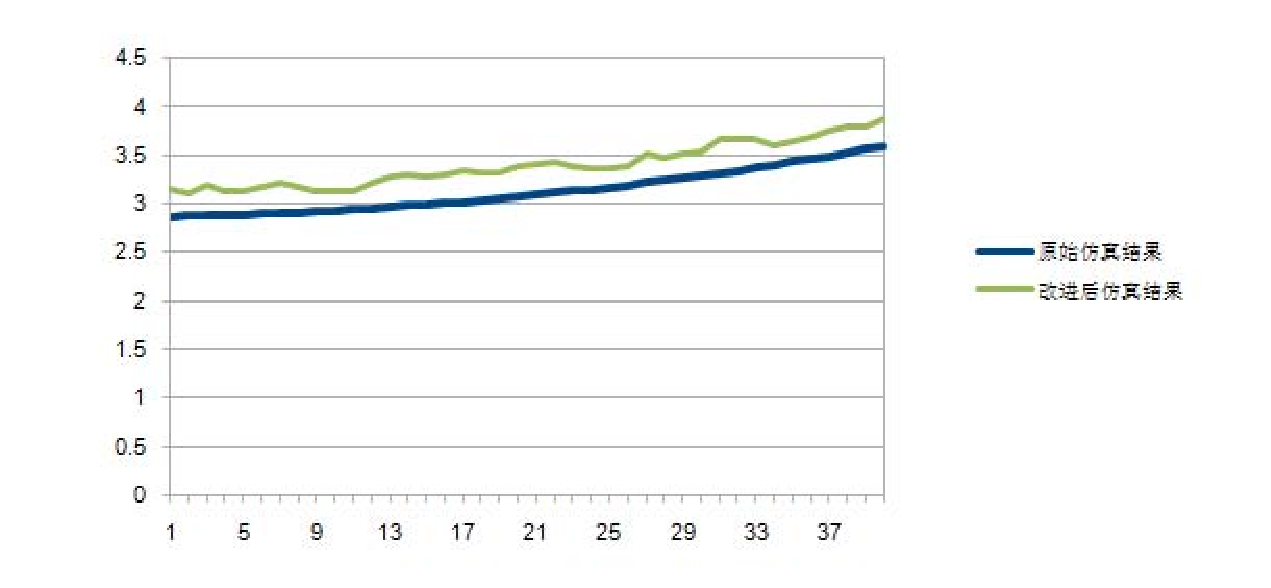
\includegraphics{improve5.pdf}}
  % GNUPLOT: LaTeX picture
\setlength{\unitlength}{0.240900pt}
\ifx\plotpoint\undefined\newsavebox{\plotpoint}\fi
\begin{picture}(1500,900)(0,0)
\sbox{\plotpoint}{\rule[-0.200pt]{0.400pt}{0.400pt}}%
\put(131.0,82.0){\rule[-0.200pt]{4.818pt}{0.400pt}}
\put(111,82){\makebox(0,0)[r]{ 0}}
\put(1419.0,82.0){\rule[-0.200pt]{4.818pt}{0.400pt}}
\put(131.0,237.0){\rule[-0.200pt]{4.818pt}{0.400pt}}
\put(111,237){\makebox(0,0)[r]{ 1}}
\put(1419.0,237.0){\rule[-0.200pt]{4.818pt}{0.400pt}}
\put(131.0,393.0){\rule[-0.200pt]{4.818pt}{0.400pt}}
\put(111,393){\makebox(0,0)[r]{ 2}}
\put(1419.0,393.0){\rule[-0.200pt]{4.818pt}{0.400pt}}
\put(131.0,548.0){\rule[-0.200pt]{4.818pt}{0.400pt}}
\put(111,548){\makebox(0,0)[r]{ 3}}
\put(1419.0,548.0){\rule[-0.200pt]{4.818pt}{0.400pt}}
\put(131.0,704.0){\rule[-0.200pt]{4.818pt}{0.400pt}}
\put(111,704){\makebox(0,0)[r]{ 4}}
\put(1419.0,704.0){\rule[-0.200pt]{4.818pt}{0.400pt}}
\put(131.0,82.0){\rule[-0.200pt]{0.400pt}{4.818pt}}
\put(131,41){\makebox(0,0){ 1}}
\put(131.0,839.0){\rule[-0.200pt]{0.400pt}{4.818pt}}
\put(198.0,82.0){\rule[-0.200pt]{0.400pt}{4.818pt}}
\put(198,41){\makebox(0,0){ 3}}
\put(198.0,839.0){\rule[-0.200pt]{0.400pt}{4.818pt}}
\put(265.0,82.0){\rule[-0.200pt]{0.400pt}{4.818pt}}
\put(265,41){\makebox(0,0){ 5}}
\put(265.0,839.0){\rule[-0.200pt]{0.400pt}{4.818pt}}
\put(332.0,82.0){\rule[-0.200pt]{0.400pt}{4.818pt}}
\put(332,41){\makebox(0,0){ 7}}
\put(332.0,839.0){\rule[-0.200pt]{0.400pt}{4.818pt}}
\put(399.0,82.0){\rule[-0.200pt]{0.400pt}{4.818pt}}
\put(399,41){\makebox(0,0){ 9}}
\put(399.0,839.0){\rule[-0.200pt]{0.400pt}{4.818pt}}
\put(466.0,82.0){\rule[-0.200pt]{0.400pt}{4.818pt}}
\put(466,41){\makebox(0,0){ 11}}
\put(466.0,839.0){\rule[-0.200pt]{0.400pt}{4.818pt}}
\put(533.0,82.0){\rule[-0.200pt]{0.400pt}{4.818pt}}
\put(533,41){\makebox(0,0){ 13}}
\put(533.0,839.0){\rule[-0.200pt]{0.400pt}{4.818pt}}
\put(601.0,82.0){\rule[-0.200pt]{0.400pt}{4.818pt}}
\put(601,41){\makebox(0,0){ 15}}
\put(601.0,839.0){\rule[-0.200pt]{0.400pt}{4.818pt}}
\put(668.0,82.0){\rule[-0.200pt]{0.400pt}{4.818pt}}
\put(668,41){\makebox(0,0){ 17}}
\put(668.0,839.0){\rule[-0.200pt]{0.400pt}{4.818pt}}
\put(735.0,82.0){\rule[-0.200pt]{0.400pt}{4.818pt}}
\put(735,41){\makebox(0,0){ 19}}
\put(735.0,839.0){\rule[-0.200pt]{0.400pt}{4.818pt}}
\put(802.0,82.0){\rule[-0.200pt]{0.400pt}{4.818pt}}
\put(802,41){\makebox(0,0){ 21}}
\put(802.0,839.0){\rule[-0.200pt]{0.400pt}{4.818pt}}
\put(869.0,82.0){\rule[-0.200pt]{0.400pt}{4.818pt}}
\put(869,41){\makebox(0,0){ 23}}
\put(869.0,839.0){\rule[-0.200pt]{0.400pt}{4.818pt}}
\put(936.0,82.0){\rule[-0.200pt]{0.400pt}{4.818pt}}
\put(936,41){\makebox(0,0){ 25}}
\put(936.0,839.0){\rule[-0.200pt]{0.400pt}{4.818pt}}
\put(1003.0,82.0){\rule[-0.200pt]{0.400pt}{4.818pt}}
\put(1003,41){\makebox(0,0){ 27}}
\put(1003.0,839.0){\rule[-0.200pt]{0.400pt}{4.818pt}}
\put(1070.0,82.0){\rule[-0.200pt]{0.400pt}{4.818pt}}
\put(1070,41){\makebox(0,0){ 29}}
\put(1070.0,839.0){\rule[-0.200pt]{0.400pt}{4.818pt}}
\put(1137.0,82.0){\rule[-0.200pt]{0.400pt}{4.818pt}}
\put(1137,41){\makebox(0,0){ 31}}
\put(1137.0,839.0){\rule[-0.200pt]{0.400pt}{4.818pt}}
\put(1204.0,82.0){\rule[-0.200pt]{0.400pt}{4.818pt}}
\put(1204,41){\makebox(0,0){ 33}}
\put(1204.0,839.0){\rule[-0.200pt]{0.400pt}{4.818pt}}
\put(1271.0,82.0){\rule[-0.200pt]{0.400pt}{4.818pt}}
\put(1271,41){\makebox(0,0){ 35}}
\put(1271.0,839.0){\rule[-0.200pt]{0.400pt}{4.818pt}}
\put(1338.0,82.0){\rule[-0.200pt]{0.400pt}{4.818pt}}
\put(1338,41){\makebox(0,0){ 37}}
\put(1338.0,839.0){\rule[-0.200pt]{0.400pt}{4.818pt}}
\put(1405.0,82.0){\rule[-0.200pt]{0.400pt}{4.818pt}}
\put(1405,41){\makebox(0,0){ 39}}
\put(1405.0,839.0){\rule[-0.200pt]{0.400pt}{4.818pt}}
\put(131.0,82.0){\rule[-0.200pt]{0.400pt}{187.179pt}}
\put(131.0,82.0){\rule[-0.200pt]{315.097pt}{0.400pt}}
\put(1439.0,82.0){\rule[-0.200pt]{0.400pt}{187.179pt}}
\put(131.0,859.0){\rule[-0.200pt]{315.097pt}{0.400pt}}
\put(30,470){\makebox(0,0){\rotatebox{90}{用户贡献}}}
\put(785,-10){\makebox(0,0){月度}}
\put(1279,819){\makebox(0,0)[r]{仿真数据}}
\put(1299.0,819.0){\rule[-0.200pt]{24.090pt}{0.400pt}}
\put(1439,640){\usebox{\plotpoint}}
\multiput(1427.29,638.93)(-3.716,-0.477){7}{\rule{2.820pt}{0.115pt}}
\multiput(1433.15,639.17)(-28.147,-5.000){2}{\rule{1.410pt}{0.400pt}}
\multiput(1393.63,633.93)(-3.604,-0.477){7}{\rule{2.740pt}{0.115pt}}
\multiput(1399.31,634.17)(-27.313,-5.000){2}{\rule{1.370pt}{0.400pt}}
\multiput(1360.29,628.93)(-3.716,-0.477){7}{\rule{2.820pt}{0.115pt}}
\multiput(1366.15,629.17)(-28.147,-5.000){2}{\rule{1.410pt}{0.400pt}}
\multiput(1326.63,623.93)(-3.604,-0.477){7}{\rule{2.740pt}{0.115pt}}
\multiput(1332.31,624.17)(-27.313,-5.000){2}{\rule{1.370pt}{0.400pt}}
\multiput(1293.29,618.93)(-3.716,-0.477){7}{\rule{2.820pt}{0.115pt}}
\multiput(1299.15,619.17)(-28.147,-5.000){2}{\rule{1.410pt}{0.400pt}}
\multiput(1256.89,613.94)(-4.722,-0.468){5}{\rule{3.400pt}{0.113pt}}
\multiput(1263.94,614.17)(-25.943,-4.000){2}{\rule{1.700pt}{0.400pt}}
\multiput(1226.29,609.93)(-3.716,-0.477){7}{\rule{2.820pt}{0.115pt}}
\multiput(1232.15,610.17)(-28.147,-5.000){2}{\rule{1.410pt}{0.400pt}}
\multiput(1189.89,604.94)(-4.722,-0.468){5}{\rule{3.400pt}{0.113pt}}
\multiput(1196.94,605.17)(-25.943,-4.000){2}{\rule{1.700pt}{0.400pt}}
\multiput(1156.47,600.94)(-4.868,-0.468){5}{\rule{3.500pt}{0.113pt}}
\multiput(1163.74,601.17)(-26.736,-4.000){2}{\rule{1.750pt}{0.400pt}}
\multiput(1125.63,596.93)(-3.604,-0.477){7}{\rule{2.740pt}{0.115pt}}
\multiput(1131.31,597.17)(-27.313,-5.000){2}{\rule{1.370pt}{0.400pt}}
\multiput(1089.47,591.94)(-4.868,-0.468){5}{\rule{3.500pt}{0.113pt}}
\multiput(1096.74,592.17)(-26.736,-4.000){2}{\rule{1.750pt}{0.400pt}}
\multiput(1051.32,587.95)(-7.160,-0.447){3}{\rule{4.500pt}{0.108pt}}
\multiput(1060.66,588.17)(-23.660,-3.000){2}{\rule{2.250pt}{0.400pt}}
\multiput(1022.47,584.94)(-4.868,-0.468){5}{\rule{3.500pt}{0.113pt}}
\multiput(1029.74,585.17)(-26.736,-4.000){2}{\rule{1.750pt}{0.400pt}}
\multiput(988.47,580.94)(-4.868,-0.468){5}{\rule{3.500pt}{0.113pt}}
\multiput(995.74,581.17)(-26.736,-4.000){2}{\rule{1.750pt}{0.400pt}}
\multiput(950.32,576.95)(-7.160,-0.447){3}{\rule{4.500pt}{0.108pt}}
\multiput(959.66,577.17)(-23.660,-3.000){2}{\rule{2.250pt}{0.400pt}}
\multiput(921.47,573.94)(-4.868,-0.468){5}{\rule{3.500pt}{0.113pt}}
\multiput(928.74,574.17)(-26.736,-4.000){2}{\rule{1.750pt}{0.400pt}}
\multiput(883.32,569.95)(-7.160,-0.447){3}{\rule{4.500pt}{0.108pt}}
\multiput(892.66,570.17)(-23.660,-3.000){2}{\rule{2.250pt}{0.400pt}}
\multiput(849.77,566.95)(-7.383,-0.447){3}{\rule{4.633pt}{0.108pt}}
\multiput(859.38,567.17)(-24.383,-3.000){2}{\rule{2.317pt}{0.400pt}}
\multiput(816.32,563.95)(-7.160,-0.447){3}{\rule{4.500pt}{0.108pt}}
\multiput(825.66,564.17)(-23.660,-3.000){2}{\rule{2.250pt}{0.400pt}}
\multiput(782.77,560.95)(-7.383,-0.447){3}{\rule{4.633pt}{0.108pt}}
\multiput(792.38,561.17)(-24.383,-3.000){2}{\rule{2.317pt}{0.400pt}}
\put(735,557.17){\rule{6.700pt}{0.400pt}}
\multiput(754.09,558.17)(-19.094,-2.000){2}{\rule{3.350pt}{0.400pt}}
\multiput(715.77,555.95)(-7.383,-0.447){3}{\rule{4.633pt}{0.108pt}}
\multiput(725.38,556.17)(-24.383,-3.000){2}{\rule{2.317pt}{0.400pt}}
\multiput(682.32,552.95)(-7.160,-0.447){3}{\rule{4.500pt}{0.108pt}}
\multiput(691.66,553.17)(-23.660,-3.000){2}{\rule{2.250pt}{0.400pt}}
\put(634,549.17){\rule{6.900pt}{0.400pt}}
\multiput(653.68,550.17)(-19.679,-2.000){2}{\rule{3.450pt}{0.400pt}}
\put(601,547.17){\rule{6.700pt}{0.400pt}}
\multiput(620.09,548.17)(-19.094,-2.000){2}{\rule{3.350pt}{0.400pt}}
\put(567,545.17){\rule{6.900pt}{0.400pt}}
\multiput(586.68,546.17)(-19.679,-2.000){2}{\rule{3.450pt}{0.400pt}}
\put(533,543.17){\rule{6.900pt}{0.400pt}}
\multiput(552.68,544.17)(-19.679,-2.000){2}{\rule{3.450pt}{0.400pt}}
\put(500,541.17){\rule{6.700pt}{0.400pt}}
\multiput(519.09,542.17)(-19.094,-2.000){2}{\rule{3.350pt}{0.400pt}}
\put(466,539.17){\rule{6.900pt}{0.400pt}}
\multiput(485.68,540.17)(-19.679,-2.000){2}{\rule{3.450pt}{0.400pt}}
\put(433,537.17){\rule{6.700pt}{0.400pt}}
\multiput(452.09,538.17)(-19.094,-2.000){2}{\rule{3.350pt}{0.400pt}}
\put(399,535.67){\rule{8.191pt}{0.400pt}}
\multiput(416.00,536.17)(-17.000,-1.000){2}{\rule{4.095pt}{0.400pt}}
\put(366,534.67){\rule{7.950pt}{0.400pt}}
\multiput(382.50,535.17)(-16.500,-1.000){2}{\rule{3.975pt}{0.400pt}}
\put(332,533.17){\rule{6.900pt}{0.400pt}}
\multiput(351.68,534.17)(-19.679,-2.000){2}{\rule{3.450pt}{0.400pt}}
\put(299,531.67){\rule{7.950pt}{0.400pt}}
\multiput(315.50,532.17)(-16.500,-1.000){2}{\rule{3.975pt}{0.400pt}}
\put(265,530.67){\rule{8.191pt}{0.400pt}}
\multiput(282.00,531.17)(-17.000,-1.000){2}{\rule{4.095pt}{0.400pt}}
\put(232,529.67){\rule{7.950pt}{0.400pt}}
\multiput(248.50,530.17)(-16.500,-1.000){2}{\rule{3.975pt}{0.400pt}}
\put(165,528.67){\rule{7.950pt}{0.400pt}}
\multiput(181.50,529.17)(-16.500,-1.000){2}{\rule{3.975pt}{0.400pt}}
\put(198.0,530.0){\rule[-0.200pt]{8.191pt}{0.400pt}}
\put(131.0,529.0){\rule[-0.200pt]{8.191pt}{0.400pt}}
\put(1279,768){\makebox(0,0)[r]{改进数据}}
\put(1299.0,768.0){\rule[-0.200pt]{24.090pt}{0.400pt}}
\put(1439,659){\usebox{\plotpoint}}
\multiput(1432.31,657.93)(-1.951,-0.489){15}{\rule{1.611pt}{0.118pt}}
\multiput(1435.66,658.17)(-30.656,-9.000){2}{\rule{0.806pt}{0.400pt}}
\put(1372,648.17){\rule{6.700pt}{0.400pt}}
\multiput(1391.09,649.17)(-19.094,-2.000){2}{\rule{3.350pt}{0.400pt}}
\multiput(1364.53,646.93)(-2.211,-0.488){13}{\rule{1.800pt}{0.117pt}}
\multiput(1368.26,647.17)(-30.264,-8.000){2}{\rule{0.900pt}{0.400pt}}
\multiput(1319.32,638.95)(-7.160,-0.447){3}{\rule{4.500pt}{0.108pt}}
\multiput(1328.66,639.17)(-23.660,-3.000){2}{\rule{2.250pt}{0.400pt}}
\put(1271,635.67){\rule{8.191pt}{0.400pt}}
\multiput(1288.00,636.17)(-17.000,-1.000){2}{\rule{4.095pt}{0.400pt}}
\multiput(1256.89,634.94)(-4.722,-0.468){5}{\rule{3.400pt}{0.113pt}}
\multiput(1263.94,635.17)(-25.943,-4.000){2}{\rule{1.700pt}{0.400pt}}
\put(1204,630.17){\rule{6.900pt}{0.400pt}}
\multiput(1223.68,631.17)(-19.679,-2.000){2}{\rule{3.450pt}{0.400pt}}
\multiput(1198.60,628.92)(-1.534,-0.492){19}{\rule{1.300pt}{0.118pt}}
\multiput(1201.30,629.17)(-30.302,-11.000){2}{\rule{0.650pt}{0.400pt}}
\multiput(1122.89,617.94)(-4.722,-0.468){5}{\rule{3.400pt}{0.113pt}}
\multiput(1129.94,618.17)(-25.943,-4.000){2}{\rule{1.700pt}{0.400pt}}
\put(1137.0,619.0){\rule[-0.200pt]{8.191pt}{0.400pt}}
\multiput(1058.63,613.93)(-3.604,-0.477){7}{\rule{2.740pt}{0.115pt}}
\multiput(1064.31,614.17)(-27.313,-5.000){2}{\rule{1.370pt}{0.400pt}}
\multiput(1025.29,608.93)(-3.716,-0.477){7}{\rule{2.820pt}{0.115pt}}
\multiput(1031.15,609.17)(-28.147,-5.000){2}{\rule{1.410pt}{0.400pt}}
\put(969,603.17){\rule{6.900pt}{0.400pt}}
\multiput(988.68,604.17)(-19.679,-2.000){2}{\rule{3.450pt}{0.400pt}}
\multiput(963.60,601.92)(-1.534,-0.492){19}{\rule{1.300pt}{0.118pt}}
\multiput(966.30,602.17)(-30.302,-11.000){2}{\rule{0.650pt}{0.400pt}}
\put(902,590.67){\rule{8.191pt}{0.400pt}}
\multiput(919.00,591.17)(-17.000,-1.000){2}{\rule{4.095pt}{0.400pt}}
\multiput(883.32,589.95)(-7.160,-0.447){3}{\rule{4.500pt}{0.108pt}}
\multiput(892.66,590.17)(-23.660,-3.000){2}{\rule{2.250pt}{0.400pt}}
\multiput(849.77,586.95)(-7.383,-0.447){3}{\rule{4.633pt}{0.108pt}}
\multiput(859.38,587.17)(-24.383,-3.000){2}{\rule{2.317pt}{0.400pt}}
\multiput(826.76,583.93)(-2.476,-0.485){11}{\rule{1.986pt}{0.117pt}}
\multiput(830.88,584.17)(-28.879,-7.000){2}{\rule{0.993pt}{0.400pt}}
\multiput(782.77,578.61)(-7.383,0.447){3}{\rule{4.633pt}{0.108pt}}
\multiput(792.38,577.17)(-24.383,3.000){2}{\rule{2.317pt}{0.400pt}}
\multiput(759.76,579.93)(-2.476,-0.485){11}{\rule{1.986pt}{0.117pt}}
\multiput(763.88,580.17)(-28.879,-7.000){2}{\rule{0.993pt}{0.400pt}}
\multiput(715.77,572.95)(-7.383,-0.447){3}{\rule{4.633pt}{0.108pt}}
\multiput(725.38,573.17)(-24.383,-3.000){2}{\rule{2.317pt}{0.400pt}}
\put(668,569.67){\rule{7.950pt}{0.400pt}}
\multiput(684.50,570.17)(-16.500,-1.000){2}{\rule{3.975pt}{0.400pt}}
\put(1070.0,615.0){\rule[-0.200pt]{8.191pt}{0.400pt}}
\multiput(586.47,568.94)(-4.868,-0.468){5}{\rule{3.500pt}{0.113pt}}
\multiput(593.74,569.17)(-26.736,-4.000){2}{\rule{1.750pt}{0.400pt}}
\put(533,566.17){\rule{6.900pt}{0.400pt}}
\multiput(552.68,565.17)(-19.679,2.000){2}{\rule{3.450pt}{0.400pt}}
\put(500,568.17){\rule{6.700pt}{0.400pt}}
\multiput(519.09,567.17)(-19.094,2.000){2}{\rule{3.350pt}{0.400pt}}
\multiput(485.47,568.94)(-4.868,-0.468){5}{\rule{3.500pt}{0.113pt}}
\multiput(492.74,569.17)(-26.736,-4.000){2}{\rule{1.750pt}{0.400pt}}
\put(433,565.67){\rule{7.950pt}{0.400pt}}
\multiput(449.50,565.17)(-16.500,1.000){2}{\rule{3.975pt}{0.400pt}}
\multiput(423.18,565.93)(-3.022,-0.482){9}{\rule{2.367pt}{0.116pt}}
\multiput(428.09,566.17)(-29.088,-6.000){2}{\rule{1.183pt}{0.400pt}}
\multiput(387.63,559.93)(-3.604,-0.477){7}{\rule{2.740pt}{0.115pt}}
\multiput(393.31,560.17)(-27.313,-5.000){2}{\rule{1.370pt}{0.400pt}}
\put(332,555.67){\rule{8.191pt}{0.400pt}}
\multiput(349.00,555.17)(-17.000,1.000){2}{\rule{4.095pt}{0.400pt}}
\multiput(313.32,555.95)(-7.160,-0.447){3}{\rule{4.500pt}{0.108pt}}
\multiput(322.66,556.17)(-23.660,-3.000){2}{\rule{2.250pt}{0.400pt}}
\multiput(291.53,552.93)(-2.211,-0.488){13}{\rule{1.800pt}{0.117pt}}
\multiput(295.26,553.17)(-30.264,-8.000){2}{\rule{0.900pt}{0.400pt}}
\multiput(246.32,546.61)(-7.160,0.447){3}{\rule{4.500pt}{0.108pt}}
\multiput(255.66,545.17)(-23.660,3.000){2}{\rule{2.250pt}{0.400pt}}
\multiput(224.53,547.93)(-2.211,-0.488){13}{\rule{1.800pt}{0.117pt}}
\multiput(228.26,548.17)(-30.264,-8.000){2}{\rule{0.900pt}{0.400pt}}
\multiput(179.32,539.95)(-7.160,-0.447){3}{\rule{4.500pt}{0.108pt}}
\multiput(188.66,540.17)(-23.660,-3.000){2}{\rule{2.250pt}{0.400pt}}
\multiput(156.52,536.93)(-2.552,-0.485){11}{\rule{2.043pt}{0.117pt}}
\multiput(160.76,537.17)(-29.760,-7.000){2}{\rule{1.021pt}{0.400pt}}
\put(1439,659){\makebox(0,0){$+$}}
\put(1405,650){\makebox(0,0){$+$}}
\put(1372,648){\makebox(0,0){$+$}}
\put(1338,640){\makebox(0,0){$+$}}
\put(1305,637){\makebox(0,0){$+$}}
\put(1271,636){\makebox(0,0){$+$}}
\put(1238,632){\makebox(0,0){$+$}}
\put(1204,630){\makebox(0,0){$+$}}
\put(1171,619){\makebox(0,0){$+$}}
\put(1137,619){\makebox(0,0){$+$}}
\put(1104,615){\makebox(0,0){$+$}}
\put(1070,615){\makebox(0,0){$+$}}
\put(1037,610){\makebox(0,0){$+$}}
\put(1003,605){\makebox(0,0){$+$}}
\put(969,603){\makebox(0,0){$+$}}
\put(936,592){\makebox(0,0){$+$}}
\put(902,591){\makebox(0,0){$+$}}
\put(869,588){\makebox(0,0){$+$}}
\put(835,585){\makebox(0,0){$+$}}
\put(802,578){\makebox(0,0){$+$}}
\put(768,581){\makebox(0,0){$+$}}
\put(735,574){\makebox(0,0){$+$}}
\put(701,571){\makebox(0,0){$+$}}
\put(668,570){\makebox(0,0){$+$}}
\put(634,570){\makebox(0,0){$+$}}
\put(601,570){\makebox(0,0){$+$}}
\put(567,566){\makebox(0,0){$+$}}
\put(533,568){\makebox(0,0){$+$}}
\put(500,570){\makebox(0,0){$+$}}
\put(466,566){\makebox(0,0){$+$}}
\put(433,567){\makebox(0,0){$+$}}
\put(399,561){\makebox(0,0){$+$}}
\put(366,556){\makebox(0,0){$+$}}
\put(332,557){\makebox(0,0){$+$}}
\put(299,554){\makebox(0,0){$+$}}
\put(265,546){\makebox(0,0){$+$}}
\put(232,549){\makebox(0,0){$+$}}
\put(198,541){\makebox(0,0){$+$}}
\put(165,538){\makebox(0,0){$+$}}
\put(131,531){\makebox(0,0){$+$}}
\put(1349,768){\makebox(0,0){$+$}}
\put(601.0,570.0){\rule[-0.200pt]{16.140pt}{0.400pt}}
\put(131.0,82.0){\rule[-0.200pt]{0.400pt}{187.179pt}}
\put(131.0,82.0){\rule[-0.200pt]{315.097pt}{0.400pt}}
\put(1439.0,82.0){\rule[-0.200pt]{0.400pt}{187.179pt}}
\put(131.0,859.0){\rule[-0.200pt]{315.097pt}{0.400pt}}
\end{picture}

 \caption{\small{\textbf{提升内容贡献者个体动机的仿真结果}}}
  \label{fig:improve5}
\end{figure}

图\ref{fig:improve6}是将所有的群体层次动机的初始值提升了$10\%$后的仿真结果。动机提升后个
体的贡献度同样有了一定的提高,同时随时间加速上升的趋势也要比提升前明显。
两个仿真的结果还表明,提升个体动机和人际间动机效果是一样
的。内容贡献者既重视在知识协同中获得心理上的满足感,同时也从与他人的互
动过程中获得良好的体验。

\begin{figure}[!htb]
  \centering
%  \scalebox{0.65}{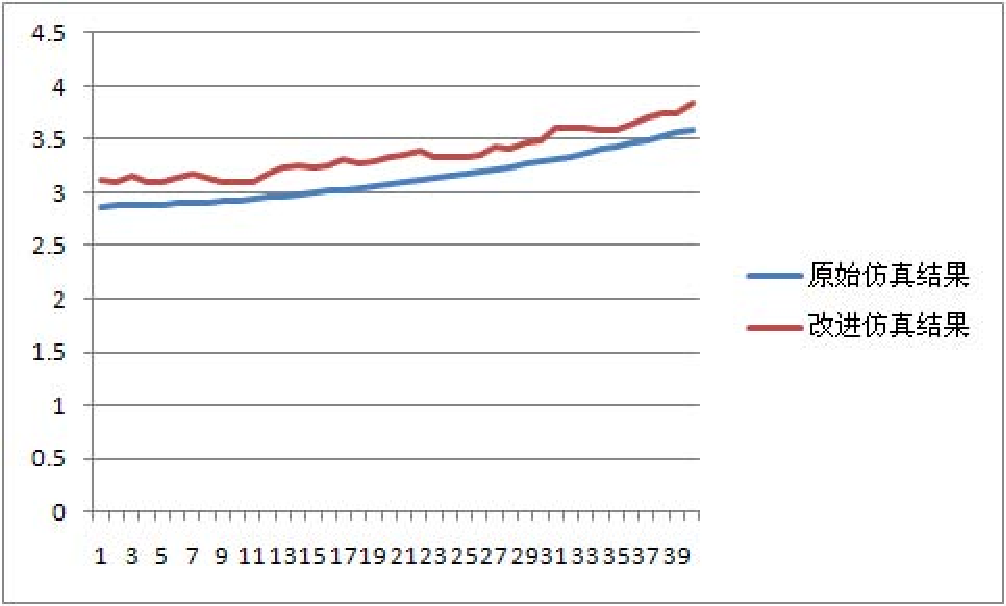
\includegraphics{improve6.pdf}}
  % GNUPLOT: LaTeX picture
\setlength{\unitlength}{0.240900pt}
\ifx\plotpoint\undefined\newsavebox{\plotpoint}\fi
\begin{picture}(1500,900)(0,0)
\sbox{\plotpoint}{\rule[-0.200pt]{0.400pt}{0.400pt}}%
\put(131.0,82.0){\rule[-0.200pt]{4.818pt}{0.400pt}}
\put(111,82){\makebox(0,0)[r]{ 0}}
\put(1419.0,82.0){\rule[-0.200pt]{4.818pt}{0.400pt}}
\put(131.0,237.0){\rule[-0.200pt]{4.818pt}{0.400pt}}
\put(111,237){\makebox(0,0)[r]{ 1}}
\put(1419.0,237.0){\rule[-0.200pt]{4.818pt}{0.400pt}}
\put(131.0,393.0){\rule[-0.200pt]{4.818pt}{0.400pt}}
\put(111,393){\makebox(0,0)[r]{ 2}}
\put(1419.0,393.0){\rule[-0.200pt]{4.818pt}{0.400pt}}
\put(131.0,548.0){\rule[-0.200pt]{4.818pt}{0.400pt}}
\put(111,548){\makebox(0,0)[r]{ 3}}
\put(1419.0,548.0){\rule[-0.200pt]{4.818pt}{0.400pt}}
\put(131.0,704.0){\rule[-0.200pt]{4.818pt}{0.400pt}}
\put(111,704){\makebox(0,0)[r]{ 4}}
\put(1419.0,704.0){\rule[-0.200pt]{4.818pt}{0.400pt}}
\put(131.0,82.0){\rule[-0.200pt]{0.400pt}{4.818pt}}
\put(131,41){\makebox(0,0){ 1}}
\put(131.0,839.0){\rule[-0.200pt]{0.400pt}{4.818pt}}
\put(198.0,82.0){\rule[-0.200pt]{0.400pt}{4.818pt}}
\put(198,41){\makebox(0,0){ 3}}
\put(198.0,839.0){\rule[-0.200pt]{0.400pt}{4.818pt}}
\put(265.0,82.0){\rule[-0.200pt]{0.400pt}{4.818pt}}
\put(265,41){\makebox(0,0){ 5}}
\put(265.0,839.0){\rule[-0.200pt]{0.400pt}{4.818pt}}
\put(332.0,82.0){\rule[-0.200pt]{0.400pt}{4.818pt}}
\put(332,41){\makebox(0,0){ 7}}
\put(332.0,839.0){\rule[-0.200pt]{0.400pt}{4.818pt}}
\put(399.0,82.0){\rule[-0.200pt]{0.400pt}{4.818pt}}
\put(399,41){\makebox(0,0){ 9}}
\put(399.0,839.0){\rule[-0.200pt]{0.400pt}{4.818pt}}
\put(466.0,82.0){\rule[-0.200pt]{0.400pt}{4.818pt}}
\put(466,41){\makebox(0,0){ 11}}
\put(466.0,839.0){\rule[-0.200pt]{0.400pt}{4.818pt}}
\put(533.0,82.0){\rule[-0.200pt]{0.400pt}{4.818pt}}
\put(533,41){\makebox(0,0){ 13}}
\put(533.0,839.0){\rule[-0.200pt]{0.400pt}{4.818pt}}
\put(601.0,82.0){\rule[-0.200pt]{0.400pt}{4.818pt}}
\put(601,41){\makebox(0,0){ 15}}
\put(601.0,839.0){\rule[-0.200pt]{0.400pt}{4.818pt}}
\put(668.0,82.0){\rule[-0.200pt]{0.400pt}{4.818pt}}
\put(668,41){\makebox(0,0){ 17}}
\put(668.0,839.0){\rule[-0.200pt]{0.400pt}{4.818pt}}
\put(735.0,82.0){\rule[-0.200pt]{0.400pt}{4.818pt}}
\put(735,41){\makebox(0,0){ 19}}
\put(735.0,839.0){\rule[-0.200pt]{0.400pt}{4.818pt}}
\put(802.0,82.0){\rule[-0.200pt]{0.400pt}{4.818pt}}
\put(802,41){\makebox(0,0){ 21}}
\put(802.0,839.0){\rule[-0.200pt]{0.400pt}{4.818pt}}
\put(869.0,82.0){\rule[-0.200pt]{0.400pt}{4.818pt}}
\put(869,41){\makebox(0,0){ 23}}
\put(869.0,839.0){\rule[-0.200pt]{0.400pt}{4.818pt}}
\put(936.0,82.0){\rule[-0.200pt]{0.400pt}{4.818pt}}
\put(936,41){\makebox(0,0){ 25}}
\put(936.0,839.0){\rule[-0.200pt]{0.400pt}{4.818pt}}
\put(1003.0,82.0){\rule[-0.200pt]{0.400pt}{4.818pt}}
\put(1003,41){\makebox(0,0){ 27}}
\put(1003.0,839.0){\rule[-0.200pt]{0.400pt}{4.818pt}}
\put(1070.0,82.0){\rule[-0.200pt]{0.400pt}{4.818pt}}
\put(1070,41){\makebox(0,0){ 29}}
\put(1070.0,839.0){\rule[-0.200pt]{0.400pt}{4.818pt}}
\put(1137.0,82.0){\rule[-0.200pt]{0.400pt}{4.818pt}}
\put(1137,41){\makebox(0,0){ 31}}
\put(1137.0,839.0){\rule[-0.200pt]{0.400pt}{4.818pt}}
\put(1204.0,82.0){\rule[-0.200pt]{0.400pt}{4.818pt}}
\put(1204,41){\makebox(0,0){ 33}}
\put(1204.0,839.0){\rule[-0.200pt]{0.400pt}{4.818pt}}
\put(1271.0,82.0){\rule[-0.200pt]{0.400pt}{4.818pt}}
\put(1271,41){\makebox(0,0){ 35}}
\put(1271.0,839.0){\rule[-0.200pt]{0.400pt}{4.818pt}}
\put(1338.0,82.0){\rule[-0.200pt]{0.400pt}{4.818pt}}
\put(1338,41){\makebox(0,0){ 37}}
\put(1338.0,839.0){\rule[-0.200pt]{0.400pt}{4.818pt}}
\put(1405.0,82.0){\rule[-0.200pt]{0.400pt}{4.818pt}}
\put(1405,41){\makebox(0,0){ 39}}
\put(1405.0,839.0){\rule[-0.200pt]{0.400pt}{4.818pt}}
\put(131.0,82.0){\rule[-0.200pt]{0.400pt}{187.179pt}}
\put(131.0,82.0){\rule[-0.200pt]{315.097pt}{0.400pt}}
\put(1439.0,82.0){\rule[-0.200pt]{0.400pt}{187.179pt}}
\put(131.0,859.0){\rule[-0.200pt]{315.097pt}{0.400pt}}
\put(30,470){\makebox(0,0){\rotatebox{90}{用户贡献}}}
\put(1279,819){\makebox(0,0)[r]{仿真数据}}
\put(1299.0,819.0){\rule[-0.200pt]{24.090pt}{0.400pt}}
\put(1439,640){\usebox{\plotpoint}}
\multiput(1427.29,638.93)(-3.716,-0.477){7}{\rule{2.820pt}{0.115pt}}
\multiput(1433.15,639.17)(-28.147,-5.000){2}{\rule{1.410pt}{0.400pt}}
\multiput(1393.63,633.93)(-3.604,-0.477){7}{\rule{2.740pt}{0.115pt}}
\multiput(1399.31,634.17)(-27.313,-5.000){2}{\rule{1.370pt}{0.400pt}}
\multiput(1360.29,628.93)(-3.716,-0.477){7}{\rule{2.820pt}{0.115pt}}
\multiput(1366.15,629.17)(-28.147,-5.000){2}{\rule{1.410pt}{0.400pt}}
\multiput(1326.63,623.93)(-3.604,-0.477){7}{\rule{2.740pt}{0.115pt}}
\multiput(1332.31,624.17)(-27.313,-5.000){2}{\rule{1.370pt}{0.400pt}}
\multiput(1293.29,618.93)(-3.716,-0.477){7}{\rule{2.820pt}{0.115pt}}
\multiput(1299.15,619.17)(-28.147,-5.000){2}{\rule{1.410pt}{0.400pt}}
\multiput(1256.89,613.94)(-4.722,-0.468){5}{\rule{3.400pt}{0.113pt}}
\multiput(1263.94,614.17)(-25.943,-4.000){2}{\rule{1.700pt}{0.400pt}}
\multiput(1226.29,609.93)(-3.716,-0.477){7}{\rule{2.820pt}{0.115pt}}
\multiput(1232.15,610.17)(-28.147,-5.000){2}{\rule{1.410pt}{0.400pt}}
\multiput(1189.89,604.94)(-4.722,-0.468){5}{\rule{3.400pt}{0.113pt}}
\multiput(1196.94,605.17)(-25.943,-4.000){2}{\rule{1.700pt}{0.400pt}}
\multiput(1156.47,600.94)(-4.868,-0.468){5}{\rule{3.500pt}{0.113pt}}
\multiput(1163.74,601.17)(-26.736,-4.000){2}{\rule{1.750pt}{0.400pt}}
\multiput(1125.63,596.93)(-3.604,-0.477){7}{\rule{2.740pt}{0.115pt}}
\multiput(1131.31,597.17)(-27.313,-5.000){2}{\rule{1.370pt}{0.400pt}}
\multiput(1089.47,591.94)(-4.868,-0.468){5}{\rule{3.500pt}{0.113pt}}
\multiput(1096.74,592.17)(-26.736,-4.000){2}{\rule{1.750pt}{0.400pt}}
\multiput(1051.32,587.95)(-7.160,-0.447){3}{\rule{4.500pt}{0.108pt}}
\multiput(1060.66,588.17)(-23.660,-3.000){2}{\rule{2.250pt}{0.400pt}}
\multiput(1022.47,584.94)(-4.868,-0.468){5}{\rule{3.500pt}{0.113pt}}
\multiput(1029.74,585.17)(-26.736,-4.000){2}{\rule{1.750pt}{0.400pt}}
\multiput(988.47,580.94)(-4.868,-0.468){5}{\rule{3.500pt}{0.113pt}}
\multiput(995.74,581.17)(-26.736,-4.000){2}{\rule{1.750pt}{0.400pt}}
\multiput(950.32,576.95)(-7.160,-0.447){3}{\rule{4.500pt}{0.108pt}}
\multiput(959.66,577.17)(-23.660,-3.000){2}{\rule{2.250pt}{0.400pt}}
\multiput(921.47,573.94)(-4.868,-0.468){5}{\rule{3.500pt}{0.113pt}}
\multiput(928.74,574.17)(-26.736,-4.000){2}{\rule{1.750pt}{0.400pt}}
\multiput(883.32,569.95)(-7.160,-0.447){3}{\rule{4.500pt}{0.108pt}}
\multiput(892.66,570.17)(-23.660,-3.000){2}{\rule{2.250pt}{0.400pt}}
\multiput(849.77,566.95)(-7.383,-0.447){3}{\rule{4.633pt}{0.108pt}}
\multiput(859.38,567.17)(-24.383,-3.000){2}{\rule{2.317pt}{0.400pt}}
\multiput(816.32,563.95)(-7.160,-0.447){3}{\rule{4.500pt}{0.108pt}}
\multiput(825.66,564.17)(-23.660,-3.000){2}{\rule{2.250pt}{0.400pt}}
\multiput(782.77,560.95)(-7.383,-0.447){3}{\rule{4.633pt}{0.108pt}}
\multiput(792.38,561.17)(-24.383,-3.000){2}{\rule{2.317pt}{0.400pt}}
\put(735,557.17){\rule{6.700pt}{0.400pt}}
\multiput(754.09,558.17)(-19.094,-2.000){2}{\rule{3.350pt}{0.400pt}}
\multiput(715.77,555.95)(-7.383,-0.447){3}{\rule{4.633pt}{0.108pt}}
\multiput(725.38,556.17)(-24.383,-3.000){2}{\rule{2.317pt}{0.400pt}}
\multiput(682.32,552.95)(-7.160,-0.447){3}{\rule{4.500pt}{0.108pt}}
\multiput(691.66,553.17)(-23.660,-3.000){2}{\rule{2.250pt}{0.400pt}}
\put(634,549.17){\rule{6.900pt}{0.400pt}}
\multiput(653.68,550.17)(-19.679,-2.000){2}{\rule{3.450pt}{0.400pt}}
\put(601,547.17){\rule{6.700pt}{0.400pt}}
\multiput(620.09,548.17)(-19.094,-2.000){2}{\rule{3.350pt}{0.400pt}}
\put(567,545.17){\rule{6.900pt}{0.400pt}}
\multiput(586.68,546.17)(-19.679,-2.000){2}{\rule{3.450pt}{0.400pt}}
\put(533,543.17){\rule{6.900pt}{0.400pt}}
\multiput(552.68,544.17)(-19.679,-2.000){2}{\rule{3.450pt}{0.400pt}}
\put(500,541.17){\rule{6.700pt}{0.400pt}}
\multiput(519.09,542.17)(-19.094,-2.000){2}{\rule{3.350pt}{0.400pt}}
\put(466,539.17){\rule{6.900pt}{0.400pt}}
\multiput(485.68,540.17)(-19.679,-2.000){2}{\rule{3.450pt}{0.400pt}}
\put(433,537.17){\rule{6.700pt}{0.400pt}}
\multiput(452.09,538.17)(-19.094,-2.000){2}{\rule{3.350pt}{0.400pt}}
\put(399,535.67){\rule{8.191pt}{0.400pt}}
\multiput(416.00,536.17)(-17.000,-1.000){2}{\rule{4.095pt}{0.400pt}}
\put(366,534.67){\rule{7.950pt}{0.400pt}}
\multiput(382.50,535.17)(-16.500,-1.000){2}{\rule{3.975pt}{0.400pt}}
\put(332,533.17){\rule{6.900pt}{0.400pt}}
\multiput(351.68,534.17)(-19.679,-2.000){2}{\rule{3.450pt}{0.400pt}}
\put(299,531.67){\rule{7.950pt}{0.400pt}}
\multiput(315.50,532.17)(-16.500,-1.000){2}{\rule{3.975pt}{0.400pt}}
\put(265,530.67){\rule{8.191pt}{0.400pt}}
\multiput(282.00,531.17)(-17.000,-1.000){2}{\rule{4.095pt}{0.400pt}}
\put(232,529.67){\rule{7.950pt}{0.400pt}}
\multiput(248.50,530.17)(-16.500,-1.000){2}{\rule{3.975pt}{0.400pt}}
\put(165,528.67){\rule{7.950pt}{0.400pt}}
\multiput(181.50,529.17)(-16.500,-1.000){2}{\rule{3.975pt}{0.400pt}}
\put(198.0,530.0){\rule[-0.200pt]{8.191pt}{0.400pt}}
\put(131.0,529.0){\rule[-0.200pt]{8.191pt}{0.400pt}}
\put(1279,768){\makebox(0,0)[r]{改进数据}}
\put(1299.0,768.0){\rule[-0.200pt]{24.090pt}{0.400pt}}
\put(131,548){\usebox{\plotpoint}}
\multiput(131.00,548.59)(2.211,0.488){13}{\rule{1.800pt}{0.117pt}}
\multiput(131.00,547.17)(30.264,8.000){2}{\rule{0.900pt}{0.400pt}}
\multiput(165.00,556.59)(2.932,0.482){9}{\rule{2.300pt}{0.116pt}}
\multiput(165.00,555.17)(28.226,6.000){2}{\rule{1.150pt}{0.400pt}}
\put(198,562.17){\rule{6.900pt}{0.400pt}}
\multiput(198.00,561.17)(19.679,2.000){2}{\rule{3.450pt}{0.400pt}}
\multiput(232.00,564.59)(2.932,0.482){9}{\rule{2.300pt}{0.116pt}}
\multiput(232.00,563.17)(28.226,6.000){2}{\rule{1.150pt}{0.400pt}}
\put(265,568.17){\rule{6.900pt}{0.400pt}}
\multiput(265.00,569.17)(19.679,-2.000){2}{\rule{3.450pt}{0.400pt}}
\put(299,568.17){\rule{6.700pt}{0.400pt}}
\multiput(299.00,567.17)(19.094,2.000){2}{\rule{3.350pt}{0.400pt}}
\put(332,570.17){\rule{6.900pt}{0.400pt}}
\multiput(332.00,569.17)(19.679,2.000){2}{\rule{3.450pt}{0.400pt}}
\put(366,571.67){\rule{7.950pt}{0.400pt}}
\multiput(366.00,571.17)(16.500,1.000){2}{\rule{3.975pt}{0.400pt}}
\multiput(399.00,573.61)(7.383,0.447){3}{\rule{4.633pt}{0.108pt}}
\multiput(399.00,572.17)(24.383,3.000){2}{\rule{2.317pt}{0.400pt}}
\put(433,576.17){\rule{6.700pt}{0.400pt}}
\multiput(433.00,575.17)(19.094,2.000){2}{\rule{3.350pt}{0.400pt}}
\multiput(466.00,576.95)(7.383,-0.447){3}{\rule{4.633pt}{0.108pt}}
\multiput(466.00,577.17)(24.383,-3.000){2}{\rule{2.317pt}{0.400pt}}
\multiput(500.00,575.59)(1.893,0.489){15}{\rule{1.567pt}{0.118pt}}
\multiput(500.00,574.17)(29.748,9.000){2}{\rule{0.783pt}{0.400pt}}
\put(533,583.67){\rule{8.191pt}{0.400pt}}
\multiput(533.00,583.17)(17.000,1.000){2}{\rule{4.095pt}{0.400pt}}
\multiput(567.00,583.95)(7.383,-0.447){3}{\rule{4.633pt}{0.108pt}}
\multiput(567.00,584.17)(24.383,-3.000){2}{\rule{2.317pt}{0.400pt}}
\multiput(601.00,582.59)(2.145,0.488){13}{\rule{1.750pt}{0.117pt}}
\multiput(601.00,581.17)(29.368,8.000){2}{\rule{0.875pt}{0.400pt}}
\multiput(634.00,590.61)(7.383,0.447){3}{\rule{4.633pt}{0.108pt}}
\multiput(634.00,589.17)(24.383,3.000){2}{\rule{2.317pt}{0.400pt}}
\put(668,591.67){\rule{7.950pt}{0.400pt}}
\multiput(668.00,592.17)(16.500,-1.000){2}{\rule{3.975pt}{0.400pt}}
\multiput(701.00,592.61)(7.383,0.447){3}{\rule{4.633pt}{0.108pt}}
\multiput(701.00,591.17)(24.383,3.000){2}{\rule{2.317pt}{0.400pt}}
\multiput(735.00,595.61)(7.160,0.447){3}{\rule{4.500pt}{0.108pt}}
\multiput(735.00,594.17)(23.660,3.000){2}{\rule{2.250pt}{0.400pt}}
\put(768,597.67){\rule{8.191pt}{0.400pt}}
\multiput(768.00,597.17)(17.000,1.000){2}{\rule{4.095pt}{0.400pt}}
\put(802,599.17){\rule{6.700pt}{0.400pt}}
\multiput(802.00,598.17)(19.094,2.000){2}{\rule{3.350pt}{0.400pt}}
\multiput(835.00,601.59)(3.716,0.477){7}{\rule{2.820pt}{0.115pt}}
\multiput(835.00,600.17)(28.147,5.000){2}{\rule{1.410pt}{0.400pt}}
\put(869,605.67){\rule{7.950pt}{0.400pt}}
\multiput(869.00,605.17)(16.500,1.000){2}{\rule{3.975pt}{0.400pt}}
\multiput(902.00,607.59)(3.716,0.477){7}{\rule{2.820pt}{0.115pt}}
\multiput(902.00,606.17)(28.147,5.000){2}{\rule{1.410pt}{0.400pt}}
\multiput(936.00,612.61)(7.160,0.447){3}{\rule{4.500pt}{0.108pt}}
\multiput(936.00,611.17)(23.660,3.000){2}{\rule{2.250pt}{0.400pt}}
\put(969,615.17){\rule{6.900pt}{0.400pt}}
\multiput(969.00,614.17)(19.679,2.000){2}{\rule{3.450pt}{0.400pt}}
\put(1003,615.17){\rule{6.900pt}{0.400pt}}
\multiput(1003.00,616.17)(19.679,-2.000){2}{\rule{3.450pt}{0.400pt}}
\multiput(1037.00,615.61)(7.160,0.447){3}{\rule{4.500pt}{0.108pt}}
\multiput(1037.00,614.17)(23.660,3.000){2}{\rule{2.250pt}{0.400pt}}
\put(1070,618.17){\rule{6.900pt}{0.400pt}}
\multiput(1070.00,617.17)(19.679,2.000){2}{\rule{3.450pt}{0.400pt}}
\multiput(1104.00,620.59)(2.932,0.482){9}{\rule{2.300pt}{0.116pt}}
\multiput(1104.00,619.17)(28.226,6.000){2}{\rule{1.150pt}{0.400pt}}
\multiput(1137.00,626.59)(3.022,0.482){9}{\rule{2.367pt}{0.116pt}}
\multiput(1137.00,625.17)(29.088,6.000){2}{\rule{1.183pt}{0.400pt}}
\multiput(1171.00,632.59)(2.145,0.488){13}{\rule{1.750pt}{0.117pt}}
\multiput(1171.00,631.17)(29.368,8.000){2}{\rule{0.875pt}{0.400pt}}
\put(1204,639.67){\rule{8.191pt}{0.400pt}}
\multiput(1204.00,639.17)(17.000,1.000){2}{\rule{4.095pt}{0.400pt}}
\put(1238,641.17){\rule{6.700pt}{0.400pt}}
\multiput(1238.00,640.17)(19.094,2.000){2}{\rule{3.350pt}{0.400pt}}
\multiput(1271.00,643.61)(7.383,0.447){3}{\rule{4.633pt}{0.108pt}}
\multiput(1271.00,642.17)(24.383,3.000){2}{\rule{2.317pt}{0.400pt}}
\put(1305,646.17){\rule{6.700pt}{0.400pt}}
\multiput(1305.00,645.17)(19.094,2.000){2}{\rule{3.350pt}{0.400pt}}
\multiput(1338.00,648.61)(7.383,0.447){3}{\rule{4.633pt}{0.108pt}}
\multiput(1338.00,647.17)(24.383,3.000){2}{\rule{2.317pt}{0.400pt}}
\multiput(1372.00,651.60)(4.722,0.468){5}{\rule{3.400pt}{0.113pt}}
\multiput(1372.00,650.17)(25.943,4.000){2}{\rule{1.700pt}{0.400pt}}
\put(1405,655.17){\rule{6.900pt}{0.400pt}}
\multiput(1405.00,654.17)(19.679,2.000){2}{\rule{3.450pt}{0.400pt}}
\put(131,548){\makebox(0,0){$+$}}
\put(165,556){\makebox(0,0){$+$}}
\put(198,562){\makebox(0,0){$+$}}
\put(232,564){\makebox(0,0){$+$}}
\put(265,570){\makebox(0,0){$+$}}
\put(299,568){\makebox(0,0){$+$}}
\put(332,570){\makebox(0,0){$+$}}
\put(366,572){\makebox(0,0){$+$}}
\put(399,573){\makebox(0,0){$+$}}
\put(433,576){\makebox(0,0){$+$}}
\put(466,578){\makebox(0,0){$+$}}
\put(500,575){\makebox(0,0){$+$}}
\put(533,584){\makebox(0,0){$+$}}
\put(567,585){\makebox(0,0){$+$}}
\put(601,582){\makebox(0,0){$+$}}
\put(634,590){\makebox(0,0){$+$}}
\put(668,593){\makebox(0,0){$+$}}
\put(701,592){\makebox(0,0){$+$}}
\put(735,595){\makebox(0,0){$+$}}
\put(768,598){\makebox(0,0){$+$}}
\put(802,599){\makebox(0,0){$+$}}
\put(835,601){\makebox(0,0){$+$}}
\put(869,606){\makebox(0,0){$+$}}
\put(902,607){\makebox(0,0){$+$}}
\put(936,612){\makebox(0,0){$+$}}
\put(969,615){\makebox(0,0){$+$}}
\put(1003,617){\makebox(0,0){$+$}}
\put(1037,615){\makebox(0,0){$+$}}
\put(1070,618){\makebox(0,0){$+$}}
\put(1104,620){\makebox(0,0){$+$}}
\put(1137,626){\makebox(0,0){$+$}}
\put(1171,632){\makebox(0,0){$+$}}
\put(1204,640){\makebox(0,0){$+$}}
\put(1238,641){\makebox(0,0){$+$}}
\put(1271,643){\makebox(0,0){$+$}}
\put(1305,646){\makebox(0,0){$+$}}
\put(1338,648){\makebox(0,0){$+$}}
\put(1372,651){\makebox(0,0){$+$}}
\put(1405,655){\makebox(0,0){$+$}}
\put(1439,657){\makebox(0,0){$+$}}
\put(1349,768){\makebox(0,0){$+$}}
\put(131.0,82.0){\rule[-0.200pt]{0.400pt}{187.179pt}}
\put(131.0,82.0){\rule[-0.200pt]{315.097pt}{0.400pt}}
\put(1439.0,82.0){\rule[-0.200pt]{0.400pt}{187.179pt}}
\put(131.0,859.0){\rule[-0.200pt]{315.097pt}{0.400pt}}
\end{picture}

  \caption{\small{\textbf{提升内容贡献者人际间动机的仿真结果}}}
  \label{fig:improve6}
\end{figure}

社区对于内容贡献者的激励可以从两方面展开。一方面,社区应该积极鼓励内容
协同者,重视他们的工作并及时给予积极的反馈,促进内容协同者动机水平的迅
速提升。另一方面,这类用户具有对社区的从属和依赖感,因此社区应采取措施
保护用户对社区的感情。尤其是当社区的规模不断扩大时,其他用户各种不合意的行为会
不断涌现出来,而内容贡献者对他人的行为要比领导者敏感的多。不断指定各种
制度、规定保障知识协同的顺利开展,已有的成果不被破坏,是保证内容贡献者
的知识协同动机不断提升的保证。

\subsection{内容维护者}
内容维护者在社区中属于积极参与,但是贡献水平较低,工作质量较差的群体。
其编辑的内容受到认可的程度要远远低于前三类用户。根据统计结果,内容维护
者的总贡献只相当于其正贡献值的$60\%$,这意味着有$40\%$的贡献未受到其他
协同者的承认。随着时间推移,负面效应
累计的影响越来于多,使得其月人均贡献度不断下降。仿真的结果显示贡献度呈
对数下降趋势,证明负反馈对其协同水平其主要作用。

负反馈之所以能够占据主导地位,是因为内容维护者对于负反馈的敏感程度要大
于正反馈的敏感程度。考虑到内容维护者的贡献还是以正贡献居多,如果个体更
看重正反馈的话是不可能使贡献度不断下降的。图\ref{fig:improveX}是将所有的负反馈的转换系数
降低$35\%$后的仿真结果。降低转换系数意味着个体的负反馈的敏感程度下降,
由此可以检验其对个体动机的影响。仿真结果显示个体的贡献度变化趋势发生了
明显变化,由下降趋势转为缓慢上升,意味着正反馈占据了主导力量。

\begin{figure}[!htb]
  \centering
   % GNUPLOT: LaTeX picture
\setlength{\unitlength}{0.240900pt}
\ifx\plotpoint\undefined\newsavebox{\plotpoint}\fi
\begin{picture}(1500,900)(0,0)
\sbox{\plotpoint}{\rule[-0.200pt]{0.400pt}{0.400pt}}%
\put(131.0,82.0){\rule[-0.200pt]{4.818pt}{0.400pt}}
\put(111,82){\makebox(0,0)[r]{-1}}
\put(1419.0,82.0){\rule[-0.200pt]{4.818pt}{0.400pt}}
\put(131.0,212.0){\rule[-0.200pt]{4.818pt}{0.400pt}}
\put(111,212){\makebox(0,0)[r]{ 0}}
\put(1419.0,212.0){\rule[-0.200pt]{4.818pt}{0.400pt}}
\put(131.0,341.0){\rule[-0.200pt]{4.818pt}{0.400pt}}
\put(111,341){\makebox(0,0)[r]{ 1}}
\put(1419.0,341.0){\rule[-0.200pt]{4.818pt}{0.400pt}}
\put(131.0,471.0){\rule[-0.200pt]{4.818pt}{0.400pt}}
\put(111,471){\makebox(0,0)[r]{ 2}}
\put(1419.0,471.0){\rule[-0.200pt]{4.818pt}{0.400pt}}
\put(131.0,600.0){\rule[-0.200pt]{4.818pt}{0.400pt}}
\put(111,600){\makebox(0,0)[r]{ 3}}
\put(1419.0,600.0){\rule[-0.200pt]{4.818pt}{0.400pt}}
\put(131.0,730.0){\rule[-0.200pt]{4.818pt}{0.400pt}}
\put(111,730){\makebox(0,0)[r]{ 4}}
\put(1419.0,730.0){\rule[-0.200pt]{4.818pt}{0.400pt}}
\put(131.0,82.0){\rule[-0.200pt]{0.400pt}{4.818pt}}
\put(131,41){\makebox(0,0){ 1}}
\put(131.0,839.0){\rule[-0.200pt]{0.400pt}{4.818pt}}
\put(198.0,82.0){\rule[-0.200pt]{0.400pt}{4.818pt}}
\put(198,41){\makebox(0,0){ 3}}
\put(198.0,839.0){\rule[-0.200pt]{0.400pt}{4.818pt}}
\put(265.0,82.0){\rule[-0.200pt]{0.400pt}{4.818pt}}
\put(265,41){\makebox(0,0){ 5}}
\put(265.0,839.0){\rule[-0.200pt]{0.400pt}{4.818pt}}
\put(332.0,82.0){\rule[-0.200pt]{0.400pt}{4.818pt}}
\put(332,41){\makebox(0,0){ 7}}
\put(332.0,839.0){\rule[-0.200pt]{0.400pt}{4.818pt}}
\put(399.0,82.0){\rule[-0.200pt]{0.400pt}{4.818pt}}
\put(399,41){\makebox(0,0){ 9}}
\put(399.0,839.0){\rule[-0.200pt]{0.400pt}{4.818pt}}
\put(466.0,82.0){\rule[-0.200pt]{0.400pt}{4.818pt}}
\put(466,41){\makebox(0,0){ 11}}
\put(466.0,839.0){\rule[-0.200pt]{0.400pt}{4.818pt}}
\put(533.0,82.0){\rule[-0.200pt]{0.400pt}{4.818pt}}
\put(533,41){\makebox(0,0){ 13}}
\put(533.0,839.0){\rule[-0.200pt]{0.400pt}{4.818pt}}
\put(601.0,82.0){\rule[-0.200pt]{0.400pt}{4.818pt}}
\put(601,41){\makebox(0,0){ 15}}
\put(601.0,839.0){\rule[-0.200pt]{0.400pt}{4.818pt}}
\put(668.0,82.0){\rule[-0.200pt]{0.400pt}{4.818pt}}
\put(668,41){\makebox(0,0){ 17}}
\put(668.0,839.0){\rule[-0.200pt]{0.400pt}{4.818pt}}
\put(735.0,82.0){\rule[-0.200pt]{0.400pt}{4.818pt}}
\put(735,41){\makebox(0,0){ 19}}
\put(735.0,839.0){\rule[-0.200pt]{0.400pt}{4.818pt}}
\put(802.0,82.0){\rule[-0.200pt]{0.400pt}{4.818pt}}
\put(802,41){\makebox(0,0){ 21}}
\put(802.0,839.0){\rule[-0.200pt]{0.400pt}{4.818pt}}
\put(869.0,82.0){\rule[-0.200pt]{0.400pt}{4.818pt}}
\put(869,41){\makebox(0,0){ 23}}
\put(869.0,839.0){\rule[-0.200pt]{0.400pt}{4.818pt}}
\put(936.0,82.0){\rule[-0.200pt]{0.400pt}{4.818pt}}
\put(936,41){\makebox(0,0){ 25}}
\put(936.0,839.0){\rule[-0.200pt]{0.400pt}{4.818pt}}
\put(1003.0,82.0){\rule[-0.200pt]{0.400pt}{4.818pt}}
\put(1003,41){\makebox(0,0){ 27}}
\put(1003.0,839.0){\rule[-0.200pt]{0.400pt}{4.818pt}}
\put(1070.0,82.0){\rule[-0.200pt]{0.400pt}{4.818pt}}
\put(1070,41){\makebox(0,0){ 29}}
\put(1070.0,839.0){\rule[-0.200pt]{0.400pt}{4.818pt}}
\put(1137.0,82.0){\rule[-0.200pt]{0.400pt}{4.818pt}}
\put(1137,41){\makebox(0,0){ 31}}
\put(1137.0,839.0){\rule[-0.200pt]{0.400pt}{4.818pt}}
\put(1204.0,82.0){\rule[-0.200pt]{0.400pt}{4.818pt}}
\put(1204,41){\makebox(0,0){ 33}}
\put(1204.0,839.0){\rule[-0.200pt]{0.400pt}{4.818pt}}
\put(1271.0,82.0){\rule[-0.200pt]{0.400pt}{4.818pt}}
\put(1271,41){\makebox(0,0){ 35}}
\put(1271.0,839.0){\rule[-0.200pt]{0.400pt}{4.818pt}}
\put(1338.0,82.0){\rule[-0.200pt]{0.400pt}{4.818pt}}
\put(1338,41){\makebox(0,0){ 37}}
\put(1338.0,839.0){\rule[-0.200pt]{0.400pt}{4.818pt}}
\put(1405.0,82.0){\rule[-0.200pt]{0.400pt}{4.818pt}}
\put(1405,41){\makebox(0,0){ 39}}
\put(1405.0,839.0){\rule[-0.200pt]{0.400pt}{4.818pt}}
\put(131.0,82.0){\rule[-0.200pt]{0.400pt}{187.179pt}}
\put(131.0,82.0){\rule[-0.200pt]{315.097pt}{0.400pt}}
\put(1439.0,82.0){\rule[-0.200pt]{0.400pt}{187.179pt}}
\put(131.0,859.0){\rule[-0.200pt]{315.097pt}{0.400pt}}
\put(30,470){\makebox(0,0){\rotatebox{90}{用户贡献}}}
\put(1279,819){\makebox(0,0)[r]{仿真数据}}
\put(785,-10){\makebox(0,0){月度}}
\put(1299.0,819.0){\rule[-0.200pt]{24.090pt}{0.400pt}}
\put(131,552){\usebox{\plotpoint}}
\multiput(131.58,549.44)(0.498,-0.647){65}{\rule{0.120pt}{0.618pt}}
\multiput(130.17,550.72)(34.000,-42.718){2}{\rule{0.400pt}{0.309pt}}
\multiput(165.00,506.92)(0.661,-0.497){47}{\rule{0.628pt}{0.120pt}}
\multiput(165.00,507.17)(31.697,-25.000){2}{\rule{0.314pt}{0.400pt}}
\multiput(198.00,481.92)(0.775,-0.496){41}{\rule{0.718pt}{0.120pt}}
\multiput(198.00,482.17)(32.509,-22.000){2}{\rule{0.359pt}{0.400pt}}
\multiput(232.00,459.92)(1.113,-0.494){27}{\rule{0.980pt}{0.119pt}}
\multiput(232.00,460.17)(30.966,-15.000){2}{\rule{0.490pt}{0.400pt}}
\multiput(265.00,444.92)(1.581,-0.492){19}{\rule{1.336pt}{0.118pt}}
\multiput(265.00,445.17)(31.226,-11.000){2}{\rule{0.668pt}{0.400pt}}
\multiput(299.00,433.92)(1.041,-0.494){29}{\rule{0.925pt}{0.119pt}}
\multiput(299.00,434.17)(31.080,-16.000){2}{\rule{0.463pt}{0.400pt}}
\multiput(332.00,417.93)(2.552,-0.485){11}{\rule{2.043pt}{0.117pt}}
\multiput(332.00,418.17)(29.760,-7.000){2}{\rule{1.021pt}{0.400pt}}
\multiput(366.00,410.93)(3.604,-0.477){7}{\rule{2.740pt}{0.115pt}}
\multiput(366.00,411.17)(27.313,-5.000){2}{\rule{1.370pt}{0.400pt}}
\multiput(399.00,405.92)(1.746,-0.491){17}{\rule{1.460pt}{0.118pt}}
\multiput(399.00,406.17)(30.970,-10.000){2}{\rule{0.730pt}{0.400pt}}
\multiput(433.00,395.92)(1.290,-0.493){23}{\rule{1.115pt}{0.119pt}}
\multiput(433.00,396.17)(30.685,-13.000){2}{\rule{0.558pt}{0.400pt}}
\multiput(500.00,382.94)(4.722,-0.468){5}{\rule{3.400pt}{0.113pt}}
\multiput(500.00,383.17)(25.943,-4.000){2}{\rule{1.700pt}{0.400pt}}
\multiput(533.00,378.93)(3.022,-0.482){9}{\rule{2.367pt}{0.116pt}}
\multiput(533.00,379.17)(29.088,-6.000){2}{\rule{1.183pt}{0.400pt}}
\multiput(567.00,372.95)(7.383,-0.447){3}{\rule{4.633pt}{0.108pt}}
\multiput(567.00,373.17)(24.383,-3.000){2}{\rule{2.317pt}{0.400pt}}
\multiput(601.00,369.93)(3.604,-0.477){7}{\rule{2.740pt}{0.115pt}}
\multiput(601.00,370.17)(27.313,-5.000){2}{\rule{1.370pt}{0.400pt}}
\multiput(634.00,364.94)(4.868,-0.468){5}{\rule{3.500pt}{0.113pt}}
\multiput(634.00,365.17)(26.736,-4.000){2}{\rule{1.750pt}{0.400pt}}
\multiput(668.00,360.93)(2.145,-0.488){13}{\rule{1.750pt}{0.117pt}}
\multiput(668.00,361.17)(29.368,-8.000){2}{\rule{0.875pt}{0.400pt}}
\multiput(701.00,352.95)(7.383,-0.447){3}{\rule{4.633pt}{0.108pt}}
\multiput(701.00,353.17)(24.383,-3.000){2}{\rule{2.317pt}{0.400pt}}
\multiput(735.00,349.93)(3.604,-0.477){7}{\rule{2.740pt}{0.115pt}}
\multiput(735.00,350.17)(27.313,-5.000){2}{\rule{1.370pt}{0.400pt}}
\multiput(768.00,344.93)(3.022,-0.482){9}{\rule{2.367pt}{0.116pt}}
\multiput(768.00,345.17)(29.088,-6.000){2}{\rule{1.183pt}{0.400pt}}
\put(802,340.17){\rule{6.700pt}{0.400pt}}
\multiput(802.00,339.17)(19.094,2.000){2}{\rule{3.350pt}{0.400pt}}
\multiput(835.00,340.93)(2.552,-0.485){11}{\rule{2.043pt}{0.117pt}}
\multiput(835.00,341.17)(29.760,-7.000){2}{\rule{1.021pt}{0.400pt}}
\multiput(869.00,333.93)(2.932,-0.482){9}{\rule{2.300pt}{0.116pt}}
\multiput(869.00,334.17)(28.226,-6.000){2}{\rule{1.150pt}{0.400pt}}
\put(902,327.17){\rule{6.900pt}{0.400pt}}
\multiput(902.00,328.17)(19.679,-2.000){2}{\rule{3.450pt}{0.400pt}}
\put(936,327.17){\rule{6.700pt}{0.400pt}}
\multiput(936.00,326.17)(19.094,2.000){2}{\rule{3.350pt}{0.400pt}}
\multiput(969.00,327.94)(4.868,-0.468){5}{\rule{3.500pt}{0.113pt}}
\multiput(969.00,328.17)(26.736,-4.000){2}{\rule{1.750pt}{0.400pt}}
\multiput(1003.00,323.93)(3.022,-0.482){9}{\rule{2.367pt}{0.116pt}}
\multiput(1003.00,324.17)(29.088,-6.000){2}{\rule{1.183pt}{0.400pt}}
\multiput(1037.00,317.93)(2.932,-0.482){9}{\rule{2.300pt}{0.116pt}}
\multiput(1037.00,318.17)(28.226,-6.000){2}{\rule{1.150pt}{0.400pt}}
\put(1070,311.67){\rule{8.191pt}{0.400pt}}
\multiput(1070.00,312.17)(17.000,-1.000){2}{\rule{4.095pt}{0.400pt}}
\multiput(1104.00,310.95)(7.160,-0.447){3}{\rule{4.500pt}{0.108pt}}
\multiput(1104.00,311.17)(23.660,-3.000){2}{\rule{2.250pt}{0.400pt}}
\multiput(1137.00,307.94)(4.868,-0.468){5}{\rule{3.500pt}{0.113pt}}
\multiput(1137.00,308.17)(26.736,-4.000){2}{\rule{1.750pt}{0.400pt}}
\put(466.0,384.0){\rule[-0.200pt]{8.191pt}{0.400pt}}
\put(1238,303.17){\rule{6.700pt}{0.400pt}}
\multiput(1238.00,304.17)(19.094,-2.000){2}{\rule{3.350pt}{0.400pt}}
\put(1271,301.67){\rule{8.191pt}{0.400pt}}
\multiput(1271.00,302.17)(17.000,-1.000){2}{\rule{4.095pt}{0.400pt}}
\put(1171.0,305.0){\rule[-0.200pt]{16.140pt}{0.400pt}}
\put(1338,301.67){\rule{8.191pt}{0.400pt}}
\multiput(1338.00,301.17)(17.000,1.000){2}{\rule{4.095pt}{0.400pt}}
\multiput(1372.00,301.93)(2.932,-0.482){9}{\rule{2.300pt}{0.116pt}}
\multiput(1372.00,302.17)(28.226,-6.000){2}{\rule{1.150pt}{0.400pt}}
\put(1405,295.67){\rule{8.191pt}{0.400pt}}
\multiput(1405.00,296.17)(17.000,-1.000){2}{\rule{4.095pt}{0.400pt}}
\put(1305.0,302.0){\rule[-0.200pt]{7.950pt}{0.400pt}}
\put(1279,768){\makebox(0,0)[r]{改进数据}}
\put(1299.0,768.0){\rule[-0.200pt]{24.090pt}{0.400pt}}
\put(131,583){\usebox{\plotpoint}}
\put(131,582.67){\rule{8.191pt}{0.400pt}}
\multiput(131.00,582.17)(17.000,1.000){2}{\rule{4.095pt}{0.400pt}}
\put(198,584.17){\rule{6.900pt}{0.400pt}}
\multiput(198.00,583.17)(19.679,2.000){2}{\rule{3.450pt}{0.400pt}}
\put(165.0,584.0){\rule[-0.200pt]{7.950pt}{0.400pt}}
\put(265,585.67){\rule{8.191pt}{0.400pt}}
\multiput(265.00,585.17)(17.000,1.000){2}{\rule{4.095pt}{0.400pt}}
\put(232.0,586.0){\rule[-0.200pt]{7.950pt}{0.400pt}}
\put(332,586.67){\rule{8.191pt}{0.400pt}}
\multiput(332.00,586.17)(17.000,1.000){2}{\rule{4.095pt}{0.400pt}}
\put(366,588.17){\rule{6.700pt}{0.400pt}}
\multiput(366.00,587.17)(19.094,2.000){2}{\rule{3.350pt}{0.400pt}}
\put(399,589.67){\rule{8.191pt}{0.400pt}}
\multiput(399.00,589.17)(17.000,1.000){2}{\rule{4.095pt}{0.400pt}}
\put(433,590.67){\rule{7.950pt}{0.400pt}}
\multiput(433.00,590.17)(16.500,1.000){2}{\rule{3.975pt}{0.400pt}}
\put(466,592.17){\rule{6.900pt}{0.400pt}}
\multiput(466.00,591.17)(19.679,2.000){2}{\rule{3.450pt}{0.400pt}}
\put(500,593.67){\rule{7.950pt}{0.400pt}}
\multiput(500.00,593.17)(16.500,1.000){2}{\rule{3.975pt}{0.400pt}}
\put(533,595.17){\rule{6.900pt}{0.400pt}}
\multiput(533.00,594.17)(19.679,2.000){2}{\rule{3.450pt}{0.400pt}}
\put(567,597.17){\rule{6.900pt}{0.400pt}}
\multiput(567.00,596.17)(19.679,2.000){2}{\rule{3.450pt}{0.400pt}}
\put(601,599.17){\rule{6.700pt}{0.400pt}}
\multiput(601.00,598.17)(19.094,2.000){2}{\rule{3.350pt}{0.400pt}}
\put(634,601.17){\rule{6.900pt}{0.400pt}}
\multiput(634.00,600.17)(19.679,2.000){2}{\rule{3.450pt}{0.400pt}}
\put(668,603.17){\rule{6.700pt}{0.400pt}}
\multiput(668.00,602.17)(19.094,2.000){2}{\rule{3.350pt}{0.400pt}}
\put(701,604.67){\rule{8.191pt}{0.400pt}}
\multiput(701.00,604.17)(17.000,1.000){2}{\rule{4.095pt}{0.400pt}}
\multiput(735.00,606.61)(7.160,0.447){3}{\rule{4.500pt}{0.108pt}}
\multiput(735.00,605.17)(23.660,3.000){2}{\rule{2.250pt}{0.400pt}}
\multiput(768.00,609.61)(7.383,0.447){3}{\rule{4.633pt}{0.108pt}}
\multiput(768.00,608.17)(24.383,3.000){2}{\rule{2.317pt}{0.400pt}}
\put(802,612.17){\rule{6.700pt}{0.400pt}}
\multiput(802.00,611.17)(19.094,2.000){2}{\rule{3.350pt}{0.400pt}}
\multiput(835.00,614.61)(7.383,0.447){3}{\rule{4.633pt}{0.108pt}}
\multiput(835.00,613.17)(24.383,3.000){2}{\rule{2.317pt}{0.400pt}}
\put(869,617.17){\rule{6.700pt}{0.400pt}}
\multiput(869.00,616.17)(19.094,2.000){2}{\rule{3.350pt}{0.400pt}}
\multiput(902.00,619.61)(7.383,0.447){3}{\rule{4.633pt}{0.108pt}}
\multiput(902.00,618.17)(24.383,3.000){2}{\rule{2.317pt}{0.400pt}}
\multiput(936.00,622.61)(7.160,0.447){3}{\rule{4.500pt}{0.108pt}}
\multiput(936.00,621.17)(23.660,3.000){2}{\rule{2.250pt}{0.400pt}}
\multiput(969.00,625.61)(7.383,0.447){3}{\rule{4.633pt}{0.108pt}}
\multiput(969.00,624.17)(24.383,3.000){2}{\rule{2.317pt}{0.400pt}}
\multiput(1003.00,628.61)(7.383,0.447){3}{\rule{4.633pt}{0.108pt}}
\multiput(1003.00,627.17)(24.383,3.000){2}{\rule{2.317pt}{0.400pt}}
\multiput(1037.00,631.60)(4.722,0.468){5}{\rule{3.400pt}{0.113pt}}
\multiput(1037.00,630.17)(25.943,4.000){2}{\rule{1.700pt}{0.400pt}}
\multiput(1070.00,635.61)(7.383,0.447){3}{\rule{4.633pt}{0.108pt}}
\multiput(1070.00,634.17)(24.383,3.000){2}{\rule{2.317pt}{0.400pt}}
\multiput(1104.00,638.61)(7.160,0.447){3}{\rule{4.500pt}{0.108pt}}
\multiput(1104.00,637.17)(23.660,3.000){2}{\rule{2.250pt}{0.400pt}}
\multiput(1137.00,641.61)(7.383,0.447){3}{\rule{4.633pt}{0.108pt}}
\multiput(1137.00,640.17)(24.383,3.000){2}{\rule{2.317pt}{0.400pt}}
\multiput(1171.00,644.60)(4.722,0.468){5}{\rule{3.400pt}{0.113pt}}
\multiput(1171.00,643.17)(25.943,4.000){2}{\rule{1.700pt}{0.400pt}}
\multiput(1204.00,648.60)(4.868,0.468){5}{\rule{3.500pt}{0.113pt}}
\multiput(1204.00,647.17)(26.736,4.000){2}{\rule{1.750pt}{0.400pt}}
\multiput(1238.00,652.60)(4.722,0.468){5}{\rule{3.400pt}{0.113pt}}
\multiput(1238.00,651.17)(25.943,4.000){2}{\rule{1.700pt}{0.400pt}}
\multiput(1271.00,656.60)(4.868,0.468){5}{\rule{3.500pt}{0.113pt}}
\multiput(1271.00,655.17)(26.736,4.000){2}{\rule{1.750pt}{0.400pt}}
\multiput(1305.00,660.61)(7.160,0.447){3}{\rule{4.500pt}{0.108pt}}
\multiput(1305.00,659.17)(23.660,3.000){2}{\rule{2.250pt}{0.400pt}}
\multiput(1338.00,663.60)(4.868,0.468){5}{\rule{3.500pt}{0.113pt}}
\multiput(1338.00,662.17)(26.736,4.000){2}{\rule{1.750pt}{0.400pt}}
\multiput(1372.00,667.59)(2.932,0.482){9}{\rule{2.300pt}{0.116pt}}
\multiput(1372.00,666.17)(28.226,6.000){2}{\rule{1.150pt}{0.400pt}}
\multiput(1405.00,673.61)(7.383,0.447){3}{\rule{4.633pt}{0.108pt}}
\multiput(1405.00,672.17)(24.383,3.000){2}{\rule{2.317pt}{0.400pt}}
\put(131,583){\makebox(0,0){$+$}}
\put(165,584){\makebox(0,0){$+$}}
\put(198,584){\makebox(0,0){$+$}}
\put(232,586){\makebox(0,0){$+$}}
\put(265,586){\makebox(0,0){$+$}}
\put(299,587){\makebox(0,0){$+$}}
\put(332,587){\makebox(0,0){$+$}}
\put(366,588){\makebox(0,0){$+$}}
\put(399,590){\makebox(0,0){$+$}}
\put(433,591){\makebox(0,0){$+$}}
\put(466,592){\makebox(0,0){$+$}}
\put(500,594){\makebox(0,0){$+$}}
\put(533,595){\makebox(0,0){$+$}}
\put(567,597){\makebox(0,0){$+$}}
\put(601,599){\makebox(0,0){$+$}}
\put(634,601){\makebox(0,0){$+$}}
\put(668,603){\makebox(0,0){$+$}}
\put(701,605){\makebox(0,0){$+$}}
\put(735,606){\makebox(0,0){$+$}}
\put(768,609){\makebox(0,0){$+$}}
\put(802,612){\makebox(0,0){$+$}}
\put(835,614){\makebox(0,0){$+$}}
\put(869,617){\makebox(0,0){$+$}}
\put(902,619){\makebox(0,0){$+$}}
\put(936,622){\makebox(0,0){$+$}}
\put(969,625){\makebox(0,0){$+$}}
\put(1003,628){\makebox(0,0){$+$}}
\put(1037,631){\makebox(0,0){$+$}}
\put(1070,635){\makebox(0,0){$+$}}
\put(1104,638){\makebox(0,0){$+$}}
\put(1137,641){\makebox(0,0){$+$}}
\put(1171,644){\makebox(0,0){$+$}}
\put(1204,648){\makebox(0,0){$+$}}
\put(1238,652){\makebox(0,0){$+$}}
\put(1271,656){\makebox(0,0){$+$}}
\put(1305,660){\makebox(0,0){$+$}}
\put(1338,663){\makebox(0,0){$+$}}
\put(1372,667){\makebox(0,0){$+$}}
\put(1405,673){\makebox(0,0){$+$}}
\put(1439,676){\makebox(0,0){$+$}}
\put(1349,768){\makebox(0,0){$+$}}
\put(299.0,587.0){\rule[-0.200pt]{7.950pt}{0.400pt}}
\put(131.0,82.0){\rule[-0.200pt]{0.400pt}{187.179pt}}
\put(131.0,82.0){\rule[-0.200pt]{315.097pt}{0.400pt}}
\put(1439.0,82.0){\rule[-0.200pt]{0.400pt}{187.179pt}}
\put(131.0,859.0){\rule[-0.200pt]{315.097pt}{0.400pt}}
\end{picture}

  \caption{\small{\textbf{降低内容维护者负反馈转换系数的仿真结果}}}
  \label{fig:improveX}
\end{figure}

图\ref{fig:improve7}和图\ref{fig:improve8}进一步比较了个体动机因素和人际间动机因素对内容维护者的影响。
仿真分别降低个体层次动机的负反馈的转换系数和群体层次的动机负反馈的转换
系数各$10\%$。结果显示两种方案都使负反馈的力量减小,但是人际间动机改
变的程度较大,意味着提升内容维护者的贡献度的措施针对其群体层次的动机开展会更有效。

\begin{figure}[!htb]
  \centering
 % \scalebox{0.65}{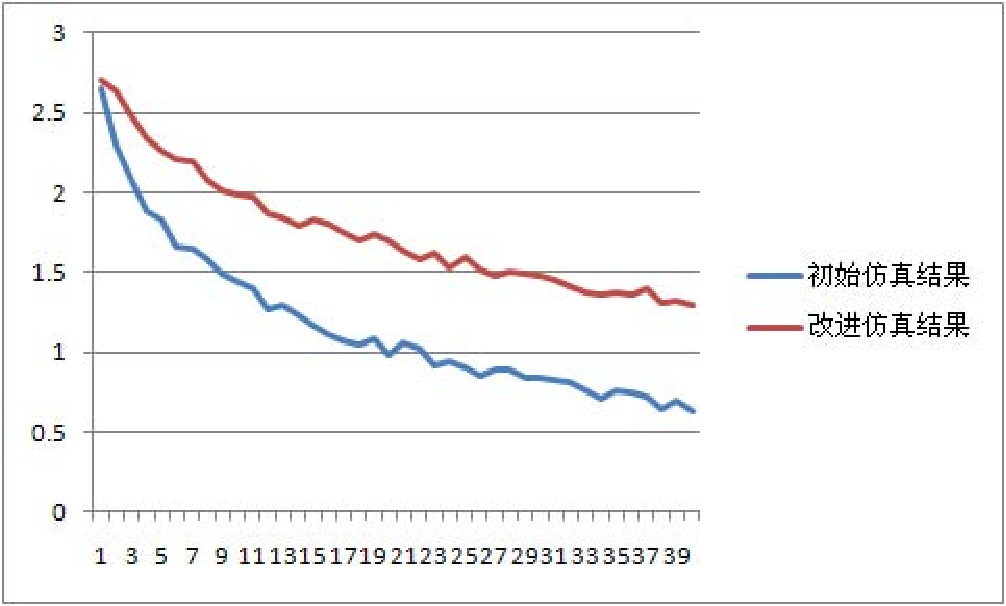
\includegraphics{improve7.pdf}}
  % GNUPLOT: LaTeX picture
\setlength{\unitlength}{0.240900pt}
\ifx\plotpoint\undefined\newsavebox{\plotpoint}\fi
\sbox{\plotpoint}{\rule[-0.200pt]{0.400pt}{0.400pt}}%
\begin{picture}(1500,900)(0,0)
\sbox{\plotpoint}{\rule[-0.200pt]{0.400pt}{0.400pt}}%
\put(131.0,82.0){\rule[-0.200pt]{4.818pt}{0.400pt}}
\put(111,82){\makebox(0,0)[r]{-1}}
\put(1419.0,82.0){\rule[-0.200pt]{4.818pt}{0.400pt}}
\put(131.0,237.0){\rule[-0.200pt]{4.818pt}{0.400pt}}
\put(111,237){\makebox(0,0)[r]{ 0}}
\put(1419.0,237.0){\rule[-0.200pt]{4.818pt}{0.400pt}}
\put(131.0,393.0){\rule[-0.200pt]{4.818pt}{0.400pt}}
\put(111,393){\makebox(0,0)[r]{ 1}}
\put(1419.0,393.0){\rule[-0.200pt]{4.818pt}{0.400pt}}
\put(131.0,548.0){\rule[-0.200pt]{4.818pt}{0.400pt}}
\put(111,548){\makebox(0,0)[r]{ 2}}
\put(1419.0,548.0){\rule[-0.200pt]{4.818pt}{0.400pt}}
\put(131.0,704.0){\rule[-0.200pt]{4.818pt}{0.400pt}}
\put(111,704){\makebox(0,0)[r]{ 3}}
\put(1419.0,704.0){\rule[-0.200pt]{4.818pt}{0.400pt}}
\put(131.0,82.0){\rule[-0.200pt]{0.400pt}{4.818pt}}
\put(131,41){\makebox(0,0){ 1}}
\put(131.0,839.0){\rule[-0.200pt]{0.400pt}{4.818pt}}
\put(198.0,82.0){\rule[-0.200pt]{0.400pt}{4.818pt}}
\put(198,41){\makebox(0,0){ 3}}
\put(198.0,839.0){\rule[-0.200pt]{0.400pt}{4.818pt}}
\put(265.0,82.0){\rule[-0.200pt]{0.400pt}{4.818pt}}
\put(265,41){\makebox(0,0){ 5}}
\put(265.0,839.0){\rule[-0.200pt]{0.400pt}{4.818pt}}
\put(332.0,82.0){\rule[-0.200pt]{0.400pt}{4.818pt}}
\put(332,41){\makebox(0,0){ 7}}
\put(332.0,839.0){\rule[-0.200pt]{0.400pt}{4.818pt}}
\put(399.0,82.0){\rule[-0.200pt]{0.400pt}{4.818pt}}
\put(399,41){\makebox(0,0){ 9}}
\put(399.0,839.0){\rule[-0.200pt]{0.400pt}{4.818pt}}
\put(466.0,82.0){\rule[-0.200pt]{0.400pt}{4.818pt}}
\put(466,41){\makebox(0,0){ 11}}
\put(466.0,839.0){\rule[-0.200pt]{0.400pt}{4.818pt}}
\put(533.0,82.0){\rule[-0.200pt]{0.400pt}{4.818pt}}
\put(533,41){\makebox(0,0){ 13}}
\put(533.0,839.0){\rule[-0.200pt]{0.400pt}{4.818pt}}
\put(601.0,82.0){\rule[-0.200pt]{0.400pt}{4.818pt}}
\put(601,41){\makebox(0,0){ 15}}
\put(601.0,839.0){\rule[-0.200pt]{0.400pt}{4.818pt}}
\put(668.0,82.0){\rule[-0.200pt]{0.400pt}{4.818pt}}
\put(668,41){\makebox(0,0){ 17}}
\put(668.0,839.0){\rule[-0.200pt]{0.400pt}{4.818pt}}
\put(735.0,82.0){\rule[-0.200pt]{0.400pt}{4.818pt}}
\put(735,41){\makebox(0,0){ 19}}
\put(735.0,839.0){\rule[-0.200pt]{0.400pt}{4.818pt}}
\put(802.0,82.0){\rule[-0.200pt]{0.400pt}{4.818pt}}
\put(802,41){\makebox(0,0){ 21}}
\put(802.0,839.0){\rule[-0.200pt]{0.400pt}{4.818pt}}
\put(869.0,82.0){\rule[-0.200pt]{0.400pt}{4.818pt}}
\put(869,41){\makebox(0,0){ 23}}
\put(869.0,839.0){\rule[-0.200pt]{0.400pt}{4.818pt}}
\put(936.0,82.0){\rule[-0.200pt]{0.400pt}{4.818pt}}
\put(936,41){\makebox(0,0){ 25}}
\put(936.0,839.0){\rule[-0.200pt]{0.400pt}{4.818pt}}
\put(1003.0,82.0){\rule[-0.200pt]{0.400pt}{4.818pt}}
\put(1003,41){\makebox(0,0){ 27}}
\put(1003.0,839.0){\rule[-0.200pt]{0.400pt}{4.818pt}}
\put(1070.0,82.0){\rule[-0.200pt]{0.400pt}{4.818pt}}
\put(1070,41){\makebox(0,0){ 29}}
\put(1070.0,839.0){\rule[-0.200pt]{0.400pt}{4.818pt}}
\put(1137.0,82.0){\rule[-0.200pt]{0.400pt}{4.818pt}}
\put(1137,41){\makebox(0,0){ 31}}
\put(1137.0,839.0){\rule[-0.200pt]{0.400pt}{4.818pt}}
\put(1204.0,82.0){\rule[-0.200pt]{0.400pt}{4.818pt}}
\put(1204,41){\makebox(0,0){ 33}}
\put(1204.0,839.0){\rule[-0.200pt]{0.400pt}{4.818pt}}
\put(1271.0,82.0){\rule[-0.200pt]{0.400pt}{4.818pt}}
\put(1271,41){\makebox(0,0){ 35}}
\put(1271.0,839.0){\rule[-0.200pt]{0.400pt}{4.818pt}}
\put(1338.0,82.0){\rule[-0.200pt]{0.400pt}{4.818pt}}
\put(1338,41){\makebox(0,0){ 37}}
\put(1338.0,839.0){\rule[-0.200pt]{0.400pt}{4.818pt}}
\put(1405.0,82.0){\rule[-0.200pt]{0.400pt}{4.818pt}}
\put(1405,41){\makebox(0,0){ 39}}
\put(1405.0,839.0){\rule[-0.200pt]{0.400pt}{4.818pt}}
\put(131.0,82.0){\rule[-0.200pt]{0.400pt}{187.179pt}}
\put(131.0,82.0){\rule[-0.200pt]{315.097pt}{0.400pt}}
\put(1439.0,82.0){\rule[-0.200pt]{0.400pt}{187.179pt}}
\put(131.0,859.0){\rule[-0.200pt]{315.097pt}{0.400pt}}
\put(30,470){\makebox(0,0){\rotatebox{90}{用户贡献}}}
\put(785,-10){\makebox(0,0){月度}}
\put(1279,819){\makebox(0,0)[r]{仿真数据}}
\put(1299.0,819.0){\rule[-0.200pt]{24.090pt}{0.400pt}}
\put(131,646){\usebox{\plotpoint}}
\multiput(131.58,643.05)(0.498,-0.766){65}{\rule{0.120pt}{0.712pt}}
\multiput(130.17,644.52)(34.000,-50.523){2}{\rule{0.400pt}{0.356pt}}
\multiput(165.00,592.92)(0.549,-0.497){57}{\rule{0.540pt}{0.120pt}}
\multiput(165.00,593.17)(31.879,-30.000){2}{\rule{0.270pt}{0.400pt}}
\multiput(198.00,562.92)(0.607,-0.497){53}{\rule{0.586pt}{0.120pt}}
\multiput(198.00,563.17)(32.784,-28.000){2}{\rule{0.293pt}{0.400pt}}
\multiput(232.00,534.92)(0.979,-0.495){31}{\rule{0.876pt}{0.119pt}}
\multiput(232.00,535.17)(31.181,-17.000){2}{\rule{0.438pt}{0.400pt}}
\multiput(265.00,517.92)(1.231,-0.494){25}{\rule{1.071pt}{0.119pt}}
\multiput(265.00,518.17)(31.776,-14.000){2}{\rule{0.536pt}{0.400pt}}
\multiput(299.00,503.92)(0.874,-0.495){35}{\rule{0.795pt}{0.119pt}}
\multiput(299.00,504.17)(31.350,-19.000){2}{\rule{0.397pt}{0.400pt}}
\multiput(332.00,484.93)(2.211,-0.488){13}{\rule{1.800pt}{0.117pt}}
\multiput(332.00,485.17)(30.264,-8.000){2}{\rule{0.900pt}{0.400pt}}
\multiput(366.00,476.93)(3.604,-0.477){7}{\rule{2.740pt}{0.115pt}}
\multiput(366.00,477.17)(27.313,-5.000){2}{\rule{1.370pt}{0.400pt}}
\multiput(399.00,471.92)(1.329,-0.493){23}{\rule{1.146pt}{0.119pt}}
\multiput(399.00,472.17)(31.621,-13.000){2}{\rule{0.573pt}{0.400pt}}
\multiput(433.00,458.92)(1.041,-0.494){29}{\rule{0.925pt}{0.119pt}}
\multiput(433.00,459.17)(31.080,-16.000){2}{\rule{0.463pt}{0.400pt}}
\put(466,443.67){\rule{8.191pt}{0.400pt}}
\multiput(466.00,443.17)(17.000,1.000){2}{\rule{4.095pt}{0.400pt}}
\multiput(500.00,443.93)(3.604,-0.477){7}{\rule{2.740pt}{0.115pt}}
\multiput(500.00,444.17)(27.313,-5.000){2}{\rule{1.370pt}{0.400pt}}
\multiput(533.00,438.93)(2.552,-0.485){11}{\rule{2.043pt}{0.117pt}}
\multiput(533.00,439.17)(29.760,-7.000){2}{\rule{1.021pt}{0.400pt}}
\multiput(567.00,431.93)(3.716,-0.477){7}{\rule{2.820pt}{0.115pt}}
\multiput(567.00,432.17)(28.147,-5.000){2}{\rule{1.410pt}{0.400pt}}
\multiput(601.00,426.93)(3.604,-0.477){7}{\rule{2.740pt}{0.115pt}}
\multiput(601.00,427.17)(27.313,-5.000){2}{\rule{1.370pt}{0.400pt}}
\multiput(634.00,421.93)(3.716,-0.477){7}{\rule{2.820pt}{0.115pt}}
\multiput(634.00,422.17)(28.147,-5.000){2}{\rule{1.410pt}{0.400pt}}
\multiput(668.00,416.93)(1.893,-0.489){15}{\rule{1.567pt}{0.118pt}}
\multiput(668.00,417.17)(29.748,-9.000){2}{\rule{0.783pt}{0.400pt}}
\multiput(701.00,407.94)(4.868,-0.468){5}{\rule{3.500pt}{0.113pt}}
\multiput(701.00,408.17)(26.736,-4.000){2}{\rule{1.750pt}{0.400pt}}
\multiput(735.00,403.93)(2.932,-0.482){9}{\rule{2.300pt}{0.116pt}}
\multiput(735.00,404.17)(28.226,-6.000){2}{\rule{1.150pt}{0.400pt}}
\multiput(768.00,397.93)(2.552,-0.485){11}{\rule{2.043pt}{0.117pt}}
\multiput(768.00,398.17)(29.760,-7.000){2}{\rule{1.021pt}{0.400pt}}
\put(802,391.67){\rule{7.950pt}{0.400pt}}
\multiput(802.00,391.17)(16.500,1.000){2}{\rule{3.975pt}{0.400pt}}
\multiput(835.00,391.93)(2.211,-0.488){13}{\rule{1.800pt}{0.117pt}}
\multiput(835.00,392.17)(30.264,-8.000){2}{\rule{0.900pt}{0.400pt}}
\multiput(869.00,383.93)(2.932,-0.482){9}{\rule{2.300pt}{0.116pt}}
\multiput(869.00,384.17)(28.226,-6.000){2}{\rule{1.150pt}{0.400pt}}
\multiput(902.00,377.95)(7.383,-0.447){3}{\rule{4.633pt}{0.108pt}}
\multiput(902.00,378.17)(24.383,-3.000){2}{\rule{2.317pt}{0.400pt}}
\put(936,376.17){\rule{6.700pt}{0.400pt}}
\multiput(936.00,375.17)(19.094,2.000){2}{\rule{3.350pt}{0.400pt}}
\multiput(969.00,376.94)(4.868,-0.468){5}{\rule{3.500pt}{0.113pt}}
\multiput(969.00,377.17)(26.736,-4.000){2}{\rule{1.750pt}{0.400pt}}
\multiput(1003.00,372.93)(2.211,-0.488){13}{\rule{1.800pt}{0.117pt}}
\multiput(1003.00,373.17)(30.264,-8.000){2}{\rule{0.900pt}{0.400pt}}
\multiput(1037.00,364.93)(2.476,-0.485){11}{\rule{1.986pt}{0.117pt}}
\multiput(1037.00,365.17)(28.879,-7.000){2}{\rule{0.993pt}{0.400pt}}
\put(1070,357.67){\rule{8.191pt}{0.400pt}}
\multiput(1070.00,358.17)(17.000,-1.000){2}{\rule{4.095pt}{0.400pt}}
\multiput(1104.00,356.94)(4.722,-0.468){5}{\rule{3.400pt}{0.113pt}}
\multiput(1104.00,357.17)(25.943,-4.000){2}{\rule{1.700pt}{0.400pt}}
\multiput(1137.00,352.94)(4.868,-0.468){5}{\rule{3.500pt}{0.113pt}}
\multiput(1137.00,353.17)(26.736,-4.000){2}{\rule{1.750pt}{0.400pt}}
\put(1171,348.67){\rule{7.950pt}{0.400pt}}
\multiput(1171.00,349.17)(16.500,-1.000){2}{\rule{3.975pt}{0.400pt}}
\put(1238,347.17){\rule{6.700pt}{0.400pt}}
\multiput(1238.00,348.17)(19.094,-2.000){2}{\rule{3.350pt}{0.400pt}}
\put(1271,345.67){\rule{8.191pt}{0.400pt}}
\multiput(1271.00,346.17)(17.000,-1.000){2}{\rule{4.095pt}{0.400pt}}
\put(1305,345.67){\rule{7.950pt}{0.400pt}}
\multiput(1305.00,345.17)(16.500,1.000){2}{\rule{3.975pt}{0.400pt}}
\put(1204.0,349.0){\rule[-0.200pt]{8.191pt}{0.400pt}}
\multiput(1372.00,345.93)(2.476,-0.485){11}{\rule{1.986pt}{0.117pt}}
\multiput(1372.00,346.17)(28.879,-7.000){2}{\rule{0.993pt}{0.400pt}}
\put(1405,338.17){\rule{6.900pt}{0.400pt}}
\multiput(1405.00,339.17)(19.679,-2.000){2}{\rule{3.450pt}{0.400pt}}
\put(1338.0,347.0){\rule[-0.200pt]{8.191pt}{0.400pt}}
\put(1279,768){\makebox(0,0)[r]{改进数据}}
\put(1299.0,768.0){\rule[-0.200pt]{24.090pt}{0.400pt}}
\put(131,669){\usebox{\plotpoint}}
\multiput(131.00,667.92)(1.009,-0.495){31}{\rule{0.900pt}{0.119pt}}
\multiput(131.00,668.17)(32.132,-17.000){2}{\rule{0.450pt}{0.400pt}}
\multiput(165.00,650.92)(0.589,-0.497){53}{\rule{0.571pt}{0.120pt}}
\multiput(165.00,651.17)(31.814,-28.000){2}{\rule{0.286pt}{0.400pt}}
\multiput(198.00,622.92)(1.009,-0.495){31}{\rule{0.900pt}{0.119pt}}
\multiput(198.00,623.17)(32.132,-17.000){2}{\rule{0.450pt}{0.400pt}}
\multiput(232.00,605.93)(2.932,-0.482){9}{\rule{2.300pt}{0.116pt}}
\multiput(232.00,606.17)(28.226,-6.000){2}{\rule{1.150pt}{0.400pt}}
\multiput(265.00,599.92)(1.581,-0.492){19}{\rule{1.336pt}{0.118pt}}
\multiput(265.00,600.17)(31.226,-11.000){2}{\rule{0.668pt}{0.400pt}}
\multiput(299.00,588.92)(1.041,-0.494){29}{\rule{0.925pt}{0.119pt}}
\multiput(299.00,589.17)(31.080,-16.000){2}{\rule{0.463pt}{0.400pt}}
\multiput(332.00,572.92)(1.444,-0.492){21}{\rule{1.233pt}{0.119pt}}
\multiput(332.00,573.17)(31.440,-12.000){2}{\rule{0.617pt}{0.400pt}}
\multiput(366.00,560.92)(1.113,-0.494){27}{\rule{0.980pt}{0.119pt}}
\multiput(366.00,561.17)(30.966,-15.000){2}{\rule{0.490pt}{0.400pt}}
\multiput(399.00,545.93)(2.211,-0.488){13}{\rule{1.800pt}{0.117pt}}
\multiput(399.00,546.17)(30.264,-8.000){2}{\rule{0.900pt}{0.400pt}}
\put(433,537.17){\rule{6.700pt}{0.400pt}}
\multiput(433.00,538.17)(19.094,-2.000){2}{\rule{3.350pt}{0.400pt}}
\multiput(466.00,535.93)(1.951,-0.489){15}{\rule{1.611pt}{0.118pt}}
\multiput(466.00,536.17)(30.656,-9.000){2}{\rule{0.806pt}{0.400pt}}
\multiput(500.00,526.93)(2.145,-0.488){13}{\rule{1.750pt}{0.117pt}}
\multiput(500.00,527.17)(29.368,-8.000){2}{\rule{0.875pt}{0.400pt}}
\multiput(533.00,518.92)(1.581,-0.492){19}{\rule{1.336pt}{0.118pt}}
\multiput(533.00,519.17)(31.226,-11.000){2}{\rule{0.668pt}{0.400pt}}
\multiput(567.00,507.92)(1.147,-0.494){27}{\rule{1.007pt}{0.119pt}}
\multiput(567.00,508.17)(31.911,-15.000){2}{\rule{0.503pt}{0.400pt}}
\multiput(601.00,492.93)(2.932,-0.482){9}{\rule{2.300pt}{0.116pt}}
\multiput(601.00,493.17)(28.226,-6.000){2}{\rule{1.150pt}{0.400pt}}
\multiput(634.00,486.94)(4.868,-0.468){5}{\rule{3.500pt}{0.113pt}}
\multiput(634.00,487.17)(26.736,-4.000){2}{\rule{1.750pt}{0.400pt}}
\multiput(668.00,482.93)(2.476,-0.485){11}{\rule{1.986pt}{0.117pt}}
\multiput(668.00,483.17)(28.879,-7.000){2}{\rule{0.993pt}{0.400pt}}
\multiput(701.00,475.95)(7.383,-0.447){3}{\rule{4.633pt}{0.108pt}}
\multiput(701.00,476.17)(24.383,-3.000){2}{\rule{2.317pt}{0.400pt}}
\multiput(735.00,472.95)(7.160,-0.447){3}{\rule{4.500pt}{0.108pt}}
\multiput(735.00,473.17)(23.660,-3.000){2}{\rule{2.250pt}{0.400pt}}
\multiput(768.00,469.93)(3.716,-0.477){7}{\rule{2.820pt}{0.115pt}}
\multiput(768.00,470.17)(28.147,-5.000){2}{\rule{1.410pt}{0.400pt}}
\multiput(802.00,464.93)(2.145,-0.488){13}{\rule{1.750pt}{0.117pt}}
\multiput(802.00,465.17)(29.368,-8.000){2}{\rule{0.875pt}{0.400pt}}
\multiput(835.00,456.93)(3.716,-0.477){7}{\rule{2.820pt}{0.115pt}}
\multiput(835.00,457.17)(28.147,-5.000){2}{\rule{1.410pt}{0.400pt}}
\multiput(869.00,451.93)(1.893,-0.489){15}{\rule{1.567pt}{0.118pt}}
\multiput(869.00,452.17)(29.748,-9.000){2}{\rule{0.783pt}{0.400pt}}
\multiput(902.00,442.93)(3.022,-0.482){9}{\rule{2.367pt}{0.116pt}}
\multiput(902.00,443.17)(29.088,-6.000){2}{\rule{1.183pt}{0.400pt}}
\multiput(936.00,436.93)(2.145,-0.488){13}{\rule{1.750pt}{0.117pt}}
\multiput(936.00,437.17)(29.368,-8.000){2}{\rule{0.875pt}{0.400pt}}
\multiput(969.00,428.93)(2.211,-0.488){13}{\rule{1.800pt}{0.117pt}}
\multiput(969.00,429.17)(30.264,-8.000){2}{\rule{0.900pt}{0.400pt}}
\multiput(1003.00,420.94)(4.868,-0.468){5}{\rule{3.500pt}{0.113pt}}
\multiput(1003.00,421.17)(26.736,-4.000){2}{\rule{1.750pt}{0.400pt}}
\multiput(1037.00,416.93)(3.604,-0.477){7}{\rule{2.740pt}{0.115pt}}
\multiput(1037.00,417.17)(27.313,-5.000){2}{\rule{1.370pt}{0.400pt}}
\multiput(1070.00,411.93)(2.211,-0.488){13}{\rule{1.800pt}{0.117pt}}
\multiput(1070.00,412.17)(30.264,-8.000){2}{\rule{0.900pt}{0.400pt}}
\multiput(1104.00,403.92)(1.401,-0.492){21}{\rule{1.200pt}{0.119pt}}
\multiput(1104.00,404.17)(30.509,-12.000){2}{\rule{0.600pt}{0.400pt}}
\put(1137,391.17){\rule{6.900pt}{0.400pt}}
\multiput(1137.00,392.17)(19.679,-2.000){2}{\rule{3.450pt}{0.400pt}}
\put(1171,389.67){\rule{7.950pt}{0.400pt}}
\multiput(1171.00,390.17)(16.500,-1.000){2}{\rule{3.975pt}{0.400pt}}
\multiput(1204.00,388.93)(3.716,-0.477){7}{\rule{2.820pt}{0.115pt}}
\multiput(1204.00,389.17)(28.147,-5.000){2}{\rule{1.410pt}{0.400pt}}
\multiput(1238.00,383.95)(7.160,-0.447){3}{\rule{4.500pt}{0.108pt}}
\multiput(1238.00,384.17)(23.660,-3.000){2}{\rule{2.250pt}{0.400pt}}
\multiput(1271.00,380.93)(3.716,-0.477){7}{\rule{2.820pt}{0.115pt}}
\multiput(1271.00,381.17)(28.147,-5.000){2}{\rule{1.410pt}{0.400pt}}
\multiput(1305.00,375.93)(3.604,-0.477){7}{\rule{2.740pt}{0.115pt}}
\multiput(1305.00,376.17)(27.313,-5.000){2}{\rule{1.370pt}{0.400pt}}
\put(1338,370.67){\rule{8.191pt}{0.400pt}}
\multiput(1338.00,371.17)(17.000,-1.000){2}{\rule{4.095pt}{0.400pt}}
\put(1372,369.17){\rule{6.700pt}{0.400pt}}
\multiput(1372.00,370.17)(19.094,-2.000){2}{\rule{3.350pt}{0.400pt}}
\put(131,669){\makebox(0,0){$+$}}
\put(165,652){\makebox(0,0){$+$}}
\put(198,624){\makebox(0,0){$+$}}
\put(232,607){\makebox(0,0){$+$}}
\put(265,601){\makebox(0,0){$+$}}
\put(299,590){\makebox(0,0){$+$}}
\put(332,574){\makebox(0,0){$+$}}
\put(366,562){\makebox(0,0){$+$}}
\put(399,547){\makebox(0,0){$+$}}
\put(433,539){\makebox(0,0){$+$}}
\put(466,537){\makebox(0,0){$+$}}
\put(500,528){\makebox(0,0){$+$}}
\put(533,520){\makebox(0,0){$+$}}
\put(567,509){\makebox(0,0){$+$}}
\put(601,494){\makebox(0,0){$+$}}
\put(634,488){\makebox(0,0){$+$}}
\put(668,484){\makebox(0,0){$+$}}
\put(701,477){\makebox(0,0){$+$}}
\put(735,474){\makebox(0,0){$+$}}
\put(768,471){\makebox(0,0){$+$}}
\put(802,466){\makebox(0,0){$+$}}
\put(835,458){\makebox(0,0){$+$}}
\put(869,453){\makebox(0,0){$+$}}
\put(902,444){\makebox(0,0){$+$}}
\put(936,438){\makebox(0,0){$+$}}
\put(969,430){\makebox(0,0){$+$}}
\put(1003,422){\makebox(0,0){$+$}}
\put(1037,418){\makebox(0,0){$+$}}
\put(1070,413){\makebox(0,0){$+$}}
\put(1104,405){\makebox(0,0){$+$}}
\put(1137,393){\makebox(0,0){$+$}}
\put(1171,391){\makebox(0,0){$+$}}
\put(1204,390){\makebox(0,0){$+$}}
\put(1238,385){\makebox(0,0){$+$}}
\put(1271,382){\makebox(0,0){$+$}}
\put(1305,377){\makebox(0,0){$+$}}
\put(1338,372){\makebox(0,0){$+$}}
\put(1372,371){\makebox(0,0){$+$}}
\put(1405,369){\makebox(0,0){$+$}}
\put(1439,369){\makebox(0,0){$+$}}
\put(1349,768){\makebox(0,0){$+$}}
\put(1405.0,369.0){\rule[-0.200pt]{8.191pt}{0.400pt}}
\put(131.0,82.0){\rule[-0.200pt]{0.400pt}{187.179pt}}
\put(131.0,82.0){\rule[-0.200pt]{315.097pt}{0.400pt}}
\put(1439.0,82.0){\rule[-0.200pt]{0.400pt}{187.179pt}}
\put(131.0,859.0){\rule[-0.200pt]{315.097pt}{0.400pt}}
\end{picture}

  \caption{\small{\textbf{提升内容维护者个体动机的仿真结果}}}
  \label{fig:improve7}
\end{figure}

\begin{figure}[!htb]
  \centering
  %\scalebox{0.65}{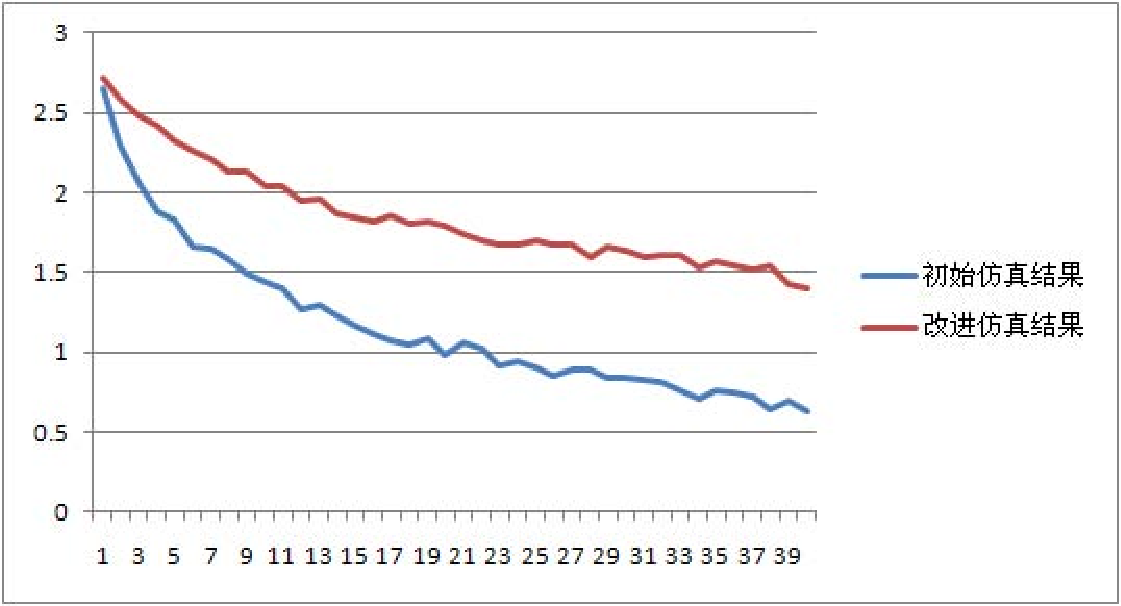
\includegraphics{improve8.pdf}}
  % GNUPLOT: LaTeX picture
\setlength{\unitlength}{0.240900pt}
\ifx\plotpoint\undefined\newsavebox{\plotpoint}\fi
\begin{picture}(1500,900)(0,0)
\sbox{\plotpoint}{\rule[-0.200pt]{0.400pt}{0.400pt}}%
\put(131.0,82.0){\rule[-0.200pt]{4.818pt}{0.400pt}}
\put(111,82){\makebox(0,0)[r]{-1}}
\put(1419.0,82.0){\rule[-0.200pt]{4.818pt}{0.400pt}}
\put(131.0,237.0){\rule[-0.200pt]{4.818pt}{0.400pt}}
\put(111,237){\makebox(0,0)[r]{ 0}}
\put(1419.0,237.0){\rule[-0.200pt]{4.818pt}{0.400pt}}
\put(131.0,393.0){\rule[-0.200pt]{4.818pt}{0.400pt}}
\put(111,393){\makebox(0,0)[r]{ 1}}
\put(1419.0,393.0){\rule[-0.200pt]{4.818pt}{0.400pt}}
\put(131.0,548.0){\rule[-0.200pt]{4.818pt}{0.400pt}}
\put(111,548){\makebox(0,0)[r]{ 2}}
\put(1419.0,548.0){\rule[-0.200pt]{4.818pt}{0.400pt}}
\put(131.0,704.0){\rule[-0.200pt]{4.818pt}{0.400pt}}
\put(111,704){\makebox(0,0)[r]{ 3}}
\put(1419.0,704.0){\rule[-0.200pt]{4.818pt}{0.400pt}}
\put(131.0,82.0){\rule[-0.200pt]{0.400pt}{4.818pt}}
\put(131,41){\makebox(0,0){ 1}}
\put(131.0,839.0){\rule[-0.200pt]{0.400pt}{4.818pt}}
\put(198.0,82.0){\rule[-0.200pt]{0.400pt}{4.818pt}}
\put(198,41){\makebox(0,0){ 3}}
\put(198.0,839.0){\rule[-0.200pt]{0.400pt}{4.818pt}}
\put(265.0,82.0){\rule[-0.200pt]{0.400pt}{4.818pt}}
\put(265,41){\makebox(0,0){ 5}}
\put(265.0,839.0){\rule[-0.200pt]{0.400pt}{4.818pt}}
\put(332.0,82.0){\rule[-0.200pt]{0.400pt}{4.818pt}}
\put(332,41){\makebox(0,0){ 7}}
\put(332.0,839.0){\rule[-0.200pt]{0.400pt}{4.818pt}}
\put(399.0,82.0){\rule[-0.200pt]{0.400pt}{4.818pt}}
\put(399,41){\makebox(0,0){ 9}}
\put(399.0,839.0){\rule[-0.200pt]{0.400pt}{4.818pt}}
\put(466.0,82.0){\rule[-0.200pt]{0.400pt}{4.818pt}}
\put(466,41){\makebox(0,0){ 11}}
\put(466.0,839.0){\rule[-0.200pt]{0.400pt}{4.818pt}}
\put(533.0,82.0){\rule[-0.200pt]{0.400pt}{4.818pt}}
\put(533,41){\makebox(0,0){ 13}}
\put(533.0,839.0){\rule[-0.200pt]{0.400pt}{4.818pt}}
\put(601.0,82.0){\rule[-0.200pt]{0.400pt}{4.818pt}}
\put(601,41){\makebox(0,0){ 15}}
\put(601.0,839.0){\rule[-0.200pt]{0.400pt}{4.818pt}}
\put(668.0,82.0){\rule[-0.200pt]{0.400pt}{4.818pt}}
\put(668,41){\makebox(0,0){ 17}}
\put(668.0,839.0){\rule[-0.200pt]{0.400pt}{4.818pt}}
\put(735.0,82.0){\rule[-0.200pt]{0.400pt}{4.818pt}}
\put(735,41){\makebox(0,0){ 19}}
\put(735.0,839.0){\rule[-0.200pt]{0.400pt}{4.818pt}}
\put(802.0,82.0){\rule[-0.200pt]{0.400pt}{4.818pt}}
\put(802,41){\makebox(0,0){ 21}}
\put(802.0,839.0){\rule[-0.200pt]{0.400pt}{4.818pt}}
\put(869.0,82.0){\rule[-0.200pt]{0.400pt}{4.818pt}}
\put(869,41){\makebox(0,0){ 23}}
\put(869.0,839.0){\rule[-0.200pt]{0.400pt}{4.818pt}}
\put(936.0,82.0){\rule[-0.200pt]{0.400pt}{4.818pt}}
\put(936,41){\makebox(0,0){ 25}}
\put(936.0,839.0){\rule[-0.200pt]{0.400pt}{4.818pt}}
\put(1003.0,82.0){\rule[-0.200pt]{0.400pt}{4.818pt}}
\put(1003,41){\makebox(0,0){ 27}}
\put(1003.0,839.0){\rule[-0.200pt]{0.400pt}{4.818pt}}
\put(1070.0,82.0){\rule[-0.200pt]{0.400pt}{4.818pt}}
\put(1070,41){\makebox(0,0){ 29}}
\put(1070.0,839.0){\rule[-0.200pt]{0.400pt}{4.818pt}}
\put(1137.0,82.0){\rule[-0.200pt]{0.400pt}{4.818pt}}
\put(1137,41){\makebox(0,0){ 31}}
\put(1137.0,839.0){\rule[-0.200pt]{0.400pt}{4.818pt}}
\put(1204.0,82.0){\rule[-0.200pt]{0.400pt}{4.818pt}}
\put(1204,41){\makebox(0,0){ 33}}
\put(1204.0,839.0){\rule[-0.200pt]{0.400pt}{4.818pt}}
\put(1271.0,82.0){\rule[-0.200pt]{0.400pt}{4.818pt}}
\put(1271,41){\makebox(0,0){ 35}}
\put(1271.0,839.0){\rule[-0.200pt]{0.400pt}{4.818pt}}
\put(1338.0,82.0){\rule[-0.200pt]{0.400pt}{4.818pt}}
\put(1338,41){\makebox(0,0){ 37}}
\put(1338.0,839.0){\rule[-0.200pt]{0.400pt}{4.818pt}}
\put(1405.0,82.0){\rule[-0.200pt]{0.400pt}{4.818pt}}
\put(1405,41){\makebox(0,0){ 39}}
\put(1405.0,839.0){\rule[-0.200pt]{0.400pt}{4.818pt}}
\put(131.0,82.0){\rule[-0.200pt]{0.400pt}{187.179pt}}
\put(131.0,82.0){\rule[-0.200pt]{315.097pt}{0.400pt}}
\put(1439.0,82.0){\rule[-0.200pt]{0.400pt}{187.179pt}}
\put(131.0,859.0){\rule[-0.200pt]{315.097pt}{0.400pt}}
\put(30,470){\makebox(0,0){\rotatebox{90}{用户贡献}}}
\put(785,-10){\makebox(0,0){月度}}
\put(1279,819){\makebox(0,0)[r]{仿真数据}}
\put(1299.0,819.0){\rule[-0.200pt]{24.090pt}{0.400pt}}
\put(131,646){\usebox{\plotpoint}}
\multiput(131.58,643.05)(0.498,-0.766){65}{\rule{0.120pt}{0.712pt}}
\multiput(130.17,644.52)(34.000,-50.523){2}{\rule{0.400pt}{0.356pt}}
\multiput(165.00,592.92)(0.549,-0.497){57}{\rule{0.540pt}{0.120pt}}
\multiput(165.00,593.17)(31.879,-30.000){2}{\rule{0.270pt}{0.400pt}}
\multiput(198.00,562.92)(0.607,-0.497){53}{\rule{0.586pt}{0.120pt}}
\multiput(198.00,563.17)(32.784,-28.000){2}{\rule{0.293pt}{0.400pt}}
\multiput(232.00,534.92)(0.979,-0.495){31}{\rule{0.876pt}{0.119pt}}
\multiput(232.00,535.17)(31.181,-17.000){2}{\rule{0.438pt}{0.400pt}}
\multiput(265.00,517.92)(1.231,-0.494){25}{\rule{1.071pt}{0.119pt}}
\multiput(265.00,518.17)(31.776,-14.000){2}{\rule{0.536pt}{0.400pt}}
\multiput(299.00,503.92)(0.874,-0.495){35}{\rule{0.795pt}{0.119pt}}
\multiput(299.00,504.17)(31.350,-19.000){2}{\rule{0.397pt}{0.400pt}}
\multiput(332.00,484.93)(2.211,-0.488){13}{\rule{1.800pt}{0.117pt}}
\multiput(332.00,485.17)(30.264,-8.000){2}{\rule{0.900pt}{0.400pt}}
\multiput(366.00,476.93)(3.604,-0.477){7}{\rule{2.740pt}{0.115pt}}
\multiput(366.00,477.17)(27.313,-5.000){2}{\rule{1.370pt}{0.400pt}}
\multiput(399.00,471.92)(1.329,-0.493){23}{\rule{1.146pt}{0.119pt}}
\multiput(399.00,472.17)(31.621,-13.000){2}{\rule{0.573pt}{0.400pt}}
\multiput(433.00,458.92)(1.041,-0.494){29}{\rule{0.925pt}{0.119pt}}
\multiput(433.00,459.17)(31.080,-16.000){2}{\rule{0.463pt}{0.400pt}}
\put(466,443.67){\rule{8.191pt}{0.400pt}}
\multiput(466.00,443.17)(17.000,1.000){2}{\rule{4.095pt}{0.400pt}}
\multiput(500.00,443.93)(3.604,-0.477){7}{\rule{2.740pt}{0.115pt}}
\multiput(500.00,444.17)(27.313,-5.000){2}{\rule{1.370pt}{0.400pt}}
\multiput(533.00,438.93)(2.552,-0.485){11}{\rule{2.043pt}{0.117pt}}
\multiput(533.00,439.17)(29.760,-7.000){2}{\rule{1.021pt}{0.400pt}}
\multiput(567.00,431.93)(3.716,-0.477){7}{\rule{2.820pt}{0.115pt}}
\multiput(567.00,432.17)(28.147,-5.000){2}{\rule{1.410pt}{0.400pt}}
\multiput(601.00,426.93)(3.604,-0.477){7}{\rule{2.740pt}{0.115pt}}
\multiput(601.00,427.17)(27.313,-5.000){2}{\rule{1.370pt}{0.400pt}}
\multiput(634.00,421.93)(3.716,-0.477){7}{\rule{2.820pt}{0.115pt}}
\multiput(634.00,422.17)(28.147,-5.000){2}{\rule{1.410pt}{0.400pt}}
\multiput(668.00,416.93)(1.893,-0.489){15}{\rule{1.567pt}{0.118pt}}
\multiput(668.00,417.17)(29.748,-9.000){2}{\rule{0.783pt}{0.400pt}}
\multiput(701.00,407.94)(4.868,-0.468){5}{\rule{3.500pt}{0.113pt}}
\multiput(701.00,408.17)(26.736,-4.000){2}{\rule{1.750pt}{0.400pt}}
\multiput(735.00,403.93)(2.932,-0.482){9}{\rule{2.300pt}{0.116pt}}
\multiput(735.00,404.17)(28.226,-6.000){2}{\rule{1.150pt}{0.400pt}}
\multiput(768.00,397.93)(2.552,-0.485){11}{\rule{2.043pt}{0.117pt}}
\multiput(768.00,398.17)(29.760,-7.000){2}{\rule{1.021pt}{0.400pt}}
\put(802,391.67){\rule{7.950pt}{0.400pt}}
\multiput(802.00,391.17)(16.500,1.000){2}{\rule{3.975pt}{0.400pt}}
\multiput(835.00,391.93)(2.211,-0.488){13}{\rule{1.800pt}{0.117pt}}
\multiput(835.00,392.17)(30.264,-8.000){2}{\rule{0.900pt}{0.400pt}}
\multiput(869.00,383.93)(2.932,-0.482){9}{\rule{2.300pt}{0.116pt}}
\multiput(869.00,384.17)(28.226,-6.000){2}{\rule{1.150pt}{0.400pt}}
\multiput(902.00,377.95)(7.383,-0.447){3}{\rule{4.633pt}{0.108pt}}
\multiput(902.00,378.17)(24.383,-3.000){2}{\rule{2.317pt}{0.400pt}}
\put(936,376.17){\rule{6.700pt}{0.400pt}}
\multiput(936.00,375.17)(19.094,2.000){2}{\rule{3.350pt}{0.400pt}}
\multiput(969.00,376.94)(4.868,-0.468){5}{\rule{3.500pt}{0.113pt}}
\multiput(969.00,377.17)(26.736,-4.000){2}{\rule{1.750pt}{0.400pt}}
\multiput(1003.00,372.93)(2.211,-0.488){13}{\rule{1.800pt}{0.117pt}}
\multiput(1003.00,373.17)(30.264,-8.000){2}{\rule{0.900pt}{0.400pt}}
\multiput(1037.00,364.93)(2.476,-0.485){11}{\rule{1.986pt}{0.117pt}}
\multiput(1037.00,365.17)(28.879,-7.000){2}{\rule{0.993pt}{0.400pt}}
\put(1070,357.67){\rule{8.191pt}{0.400pt}}
\multiput(1070.00,358.17)(17.000,-1.000){2}{\rule{4.095pt}{0.400pt}}
\multiput(1104.00,356.94)(4.722,-0.468){5}{\rule{3.400pt}{0.113pt}}
\multiput(1104.00,357.17)(25.943,-4.000){2}{\rule{1.700pt}{0.400pt}}
\multiput(1137.00,352.94)(4.868,-0.468){5}{\rule{3.500pt}{0.113pt}}
\multiput(1137.00,353.17)(26.736,-4.000){2}{\rule{1.750pt}{0.400pt}}
\put(1171,348.67){\rule{7.950pt}{0.400pt}}
\multiput(1171.00,349.17)(16.500,-1.000){2}{\rule{3.975pt}{0.400pt}}
\put(1238,347.17){\rule{6.700pt}{0.400pt}}
\multiput(1238.00,348.17)(19.094,-2.000){2}{\rule{3.350pt}{0.400pt}}
\put(1271,345.67){\rule{8.191pt}{0.400pt}}
\multiput(1271.00,346.17)(17.000,-1.000){2}{\rule{4.095pt}{0.400pt}}
\put(1305,345.67){\rule{7.950pt}{0.400pt}}
\multiput(1305.00,345.17)(16.500,1.000){2}{\rule{3.975pt}{0.400pt}}
\put(1204.0,349.0){\rule[-0.200pt]{8.191pt}{0.400pt}}
\multiput(1372.00,345.93)(2.476,-0.485){11}{\rule{1.986pt}{0.117pt}}
\multiput(1372.00,346.17)(28.879,-7.000){2}{\rule{0.993pt}{0.400pt}}
\put(1405,338.17){\rule{6.900pt}{0.400pt}}
\multiput(1405.00,339.17)(19.679,-2.000){2}{\rule{3.450pt}{0.400pt}}
\put(1338.0,347.0){\rule[-0.200pt]{8.191pt}{0.400pt}}
\put(1279,768){\makebox(0,0)[r]{改进数据}}
\put(1299.0,768.0){\rule[-0.200pt]{24.090pt}{0.400pt}}
\put(131,671){\usebox{\plotpoint}}
\multiput(131.00,669.92)(1.073,-0.494){29}{\rule{0.950pt}{0.119pt}}
\multiput(131.00,670.17)(32.028,-16.000){2}{\rule{0.475pt}{0.400pt}}
\multiput(165.00,653.92)(0.923,-0.495){33}{\rule{0.833pt}{0.119pt}}
\multiput(165.00,654.17)(31.270,-18.000){2}{\rule{0.417pt}{0.400pt}}
\multiput(198.00,635.92)(0.855,-0.496){37}{\rule{0.780pt}{0.119pt}}
\multiput(198.00,636.17)(32.381,-20.000){2}{\rule{0.390pt}{0.400pt}}
\multiput(232.00,615.93)(2.476,-0.485){11}{\rule{1.986pt}{0.117pt}}
\multiput(232.00,616.17)(28.879,-7.000){2}{\rule{0.993pt}{0.400pt}}
\multiput(265.00,608.92)(1.581,-0.492){19}{\rule{1.336pt}{0.118pt}}
\multiput(265.00,609.17)(31.226,-11.000){2}{\rule{0.668pt}{0.400pt}}
\multiput(299.00,597.92)(1.694,-0.491){17}{\rule{1.420pt}{0.118pt}}
\multiput(299.00,598.17)(30.053,-10.000){2}{\rule{0.710pt}{0.400pt}}
\multiput(332.00,587.92)(1.231,-0.494){25}{\rule{1.071pt}{0.119pt}}
\multiput(332.00,588.17)(31.776,-14.000){2}{\rule{0.536pt}{0.400pt}}
\multiput(366.00,573.92)(1.290,-0.493){23}{\rule{1.115pt}{0.119pt}}
\multiput(366.00,574.17)(30.685,-13.000){2}{\rule{0.558pt}{0.400pt}}
\multiput(399.00,560.93)(2.211,-0.488){13}{\rule{1.800pt}{0.117pt}}
\multiput(399.00,561.17)(30.264,-8.000){2}{\rule{0.900pt}{0.400pt}}
\multiput(433.00,552.93)(1.893,-0.489){15}{\rule{1.567pt}{0.118pt}}
\multiput(433.00,553.17)(29.748,-9.000){2}{\rule{0.783pt}{0.400pt}}
\multiput(466.00,543.93)(3.022,-0.482){9}{\rule{2.367pt}{0.116pt}}
\multiput(466.00,544.17)(29.088,-6.000){2}{\rule{1.183pt}{0.400pt}}
\multiput(500.00,537.93)(3.604,-0.477){7}{\rule{2.740pt}{0.115pt}}
\multiput(500.00,538.17)(27.313,-5.000){2}{\rule{1.370pt}{0.400pt}}
\multiput(533.00,532.95)(7.383,-0.447){3}{\rule{4.633pt}{0.108pt}}
\multiput(533.00,533.17)(24.383,-3.000){2}{\rule{2.317pt}{0.400pt}}
\multiput(567.00,529.93)(3.022,-0.482){9}{\rule{2.367pt}{0.116pt}}
\multiput(567.00,530.17)(29.088,-6.000){2}{\rule{1.183pt}{0.400pt}}
\multiput(601.00,523.95)(7.160,-0.447){3}{\rule{4.500pt}{0.108pt}}
\multiput(601.00,524.17)(23.660,-3.000){2}{\rule{2.250pt}{0.400pt}}
\multiput(634.00,520.92)(1.581,-0.492){19}{\rule{1.336pt}{0.118pt}}
\multiput(634.00,521.17)(31.226,-11.000){2}{\rule{0.668pt}{0.400pt}}
\multiput(668.00,509.93)(3.604,-0.477){7}{\rule{2.740pt}{0.115pt}}
\multiput(668.00,510.17)(27.313,-5.000){2}{\rule{1.370pt}{0.400pt}}
\multiput(701.00,504.93)(3.022,-0.482){9}{\rule{2.367pt}{0.116pt}}
\multiput(701.00,505.17)(29.088,-6.000){2}{\rule{1.183pt}{0.400pt}}
\multiput(735.00,498.93)(2.932,-0.482){9}{\rule{2.300pt}{0.116pt}}
\multiput(735.00,499.17)(28.226,-6.000){2}{\rule{1.150pt}{0.400pt}}
\multiput(768.00,492.93)(3.022,-0.482){9}{\rule{2.367pt}{0.116pt}}
\multiput(768.00,493.17)(29.088,-6.000){2}{\rule{1.183pt}{0.400pt}}
\multiput(802.00,486.94)(4.722,-0.468){5}{\rule{3.400pt}{0.113pt}}
\multiput(802.00,487.17)(25.943,-4.000){2}{\rule{1.700pt}{0.400pt}}
\multiput(835.00,482.92)(1.231,-0.494){25}{\rule{1.071pt}{0.119pt}}
\multiput(835.00,483.17)(31.776,-14.000){2}{\rule{0.536pt}{0.400pt}}
\multiput(869.00,468.94)(4.722,-0.468){5}{\rule{3.400pt}{0.113pt}}
\multiput(869.00,469.17)(25.943,-4.000){2}{\rule{1.700pt}{0.400pt}}
\multiput(902.00,464.93)(3.022,-0.482){9}{\rule{2.367pt}{0.116pt}}
\multiput(902.00,465.17)(29.088,-6.000){2}{\rule{1.183pt}{0.400pt}}
\multiput(936.00,458.95)(7.160,-0.447){3}{\rule{4.500pt}{0.108pt}}
\multiput(936.00,459.17)(23.660,-3.000){2}{\rule{2.250pt}{0.400pt}}
\multiput(969.00,455.93)(2.552,-0.485){11}{\rule{2.043pt}{0.117pt}}
\multiput(969.00,456.17)(29.760,-7.000){2}{\rule{1.021pt}{0.400pt}}
\multiput(1003.00,448.94)(4.868,-0.468){5}{\rule{3.500pt}{0.113pt}}
\multiput(1003.00,449.17)(26.736,-4.000){2}{\rule{1.750pt}{0.400pt}}
\multiput(1037.00,444.93)(3.604,-0.477){7}{\rule{2.740pt}{0.115pt}}
\multiput(1037.00,445.17)(27.313,-5.000){2}{\rule{1.370pt}{0.400pt}}
\multiput(1104.00,439.93)(3.604,-0.477){7}{\rule{2.740pt}{0.115pt}}
\multiput(1104.00,440.17)(27.313,-5.000){2}{\rule{1.370pt}{0.400pt}}
\multiput(1137.00,434.93)(3.022,-0.482){9}{\rule{2.367pt}{0.116pt}}
\multiput(1137.00,435.17)(29.088,-6.000){2}{\rule{1.183pt}{0.400pt}}
\multiput(1171.00,428.93)(2.932,-0.482){9}{\rule{2.300pt}{0.116pt}}
\multiput(1171.00,429.17)(28.226,-6.000){2}{\rule{1.150pt}{0.400pt}}
\multiput(1204.00,422.93)(1.951,-0.489){15}{\rule{1.611pt}{0.118pt}}
\multiput(1204.00,423.17)(30.656,-9.000){2}{\rule{0.806pt}{0.400pt}}
\multiput(1238.00,413.93)(2.476,-0.485){11}{\rule{1.986pt}{0.117pt}}
\multiput(1238.00,414.17)(28.879,-7.000){2}{\rule{0.993pt}{0.400pt}}
\multiput(1271.00,406.95)(7.383,-0.447){3}{\rule{4.633pt}{0.108pt}}
\multiput(1271.00,407.17)(24.383,-3.000){2}{\rule{2.317pt}{0.400pt}}
\multiput(1305.00,403.95)(7.160,-0.447){3}{\rule{4.500pt}{0.108pt}}
\multiput(1305.00,404.17)(23.660,-3.000){2}{\rule{2.250pt}{0.400pt}}
\multiput(1338.00,400.93)(3.022,-0.482){9}{\rule{2.367pt}{0.116pt}}
\multiput(1338.00,401.17)(29.088,-6.000){2}{\rule{1.183pt}{0.400pt}}
\put(1372,394.17){\rule{6.700pt}{0.400pt}}
\multiput(1372.00,395.17)(19.094,-2.000){2}{\rule{3.350pt}{0.400pt}}
\put(1405,392.67){\rule{8.191pt}{0.400pt}}
\multiput(1405.00,393.17)(17.000,-1.000){2}{\rule{4.095pt}{0.400pt}}
\put(131,671){\makebox(0,0){$+$}}
\put(165,655){\makebox(0,0){$+$}}
\put(198,637){\makebox(0,0){$+$}}
\put(232,617){\makebox(0,0){$+$}}
\put(265,610){\makebox(0,0){$+$}}
\put(299,599){\makebox(0,0){$+$}}
\put(332,589){\makebox(0,0){$+$}}
\put(366,575){\makebox(0,0){$+$}}
\put(399,562){\makebox(0,0){$+$}}
\put(433,554){\makebox(0,0){$+$}}
\put(466,545){\makebox(0,0){$+$}}
\put(500,539){\makebox(0,0){$+$}}
\put(533,534){\makebox(0,0){$+$}}
\put(567,531){\makebox(0,0){$+$}}
\put(601,525){\makebox(0,0){$+$}}
\put(634,522){\makebox(0,0){$+$}}
\put(668,511){\makebox(0,0){$+$}}
\put(701,506){\makebox(0,0){$+$}}
\put(735,500){\makebox(0,0){$+$}}
\put(768,494){\makebox(0,0){$+$}}
\put(802,488){\makebox(0,0){$+$}}
\put(835,484){\makebox(0,0){$+$}}
\put(869,470){\makebox(0,0){$+$}}
\put(902,466){\makebox(0,0){$+$}}
\put(936,460){\makebox(0,0){$+$}}
\put(969,457){\makebox(0,0){$+$}}
\put(1003,450){\makebox(0,0){$+$}}
\put(1037,446){\makebox(0,0){$+$}}
\put(1070,441){\makebox(0,0){$+$}}
\put(1104,441){\makebox(0,0){$+$}}
\put(1137,436){\makebox(0,0){$+$}}
\put(1171,430){\makebox(0,0){$+$}}
\put(1204,424){\makebox(0,0){$+$}}
\put(1238,415){\makebox(0,0){$+$}}
\put(1271,408){\makebox(0,0){$+$}}
\put(1305,405){\makebox(0,0){$+$}}
\put(1338,402){\makebox(0,0){$+$}}
\put(1372,396){\makebox(0,0){$+$}}
\put(1405,394){\makebox(0,0){$+$}}
\put(1439,393){\makebox(0,0){$+$}}
\put(1349,768){\makebox(0,0){$+$}}
\put(1070.0,441.0){\rule[-0.200pt]{8.191pt}{0.400pt}}
\put(131.0,82.0){\rule[-0.200pt]{0.400pt}{187.179pt}}
\put(131.0,82.0){\rule[-0.200pt]{315.097pt}{0.400pt}}
\put(1439.0,82.0){\rule[-0.200pt]{0.400pt}{187.179pt}}
\put(131.0,859.0){\rule[-0.200pt]{315.097pt}{0.400pt}}
\end{picture}

  \caption{\small{\textbf{提升内容维护者人际间动机的仿真结果}}}
  \label{fig:improve8}
\end{figure}
满足自身的社会需求是内容维护者参与社区的主要因素。内容维护者希望借由参
与社区感受到社区的温暖和支持,渴望获得社区的接纳和认同。同时,内容维护者自身的动机
水平偏低,害怕失败,尤其对于他人的行为比较敏感,动机水平容易受到外界因
素影响。这些特点决定了社区对其支持的方向应该是从保护其协同动
机入手,努力降低其对失败的关注程度,增加个体之间的协调和互动。社区管理
者应该鼓励用户之间多沟通,
多讨论,尤其是当拒绝某个人编辑的内容时应该尽力使其了解拒绝的理由、指明
改进的方向,帮助其提升编辑的水平。这样,参与者既感受到了来自于社区的支
持,同时可以将负面的感觉降低,转而多关注自身的成功,不断提升参与的信
心,使正反馈成为主导力
量。

\subsection{边缘用户}
边缘用户同内容维护者有着类似的行为模式,但是内容贡献度更低,参与次数更
少。边缘用户的月人均贡献是所有用户中唯一低于0的群体,并且变化趋势是加
速下降。边缘用户的正贡献和负贡献的比例基本是1:1,也就是说边缘用户的所
有用户贡献正负各一半,是所有用户中比例最接近的,负反馈对其的影响也是最
大的。

根据边缘用户的动机因素模型中存在着明显的负反馈环:当各体的动机降低是,
协同行为水平也会相应降低,这会导致负反馈的减少;负反馈的减少会增强个体
的动机。但是,边缘用户的行为特点显示负反馈环并未起到主导作用,这是由于
边缘用户参与的次数非常少,以至于他们不可能通过减少参与水平来达到提升个
体动机的目的。如果提升个体的动机,那么边缘用户将能够显著提升参与程度,
并转化为内容维护者,摆脱之前越不参与动机越低,动机越低越不
参与的恶性循环。

图\ref{fig:improve9}是将边缘用户的所有动机初始水平提升$30\%$所做的仿真实验。在提升初始动
机水平后,边缘用户的参与水平得到提高,并且在更多的参与中吸取了经验,熟
悉了编辑的规则和流程,提升了编辑的质量。这时边缘用户已经转化为内容贡献
者,内容贡献度的变化趋势也由加速下降转变为减速下降。仿真结果表明初始动
机水平较低是边缘用户最大的弱点,改善这一点将有助于其从社区的外围真正融
入到社区中。

\begin{figure}[!htb]
  \centering
%  \scalebox{0.65}{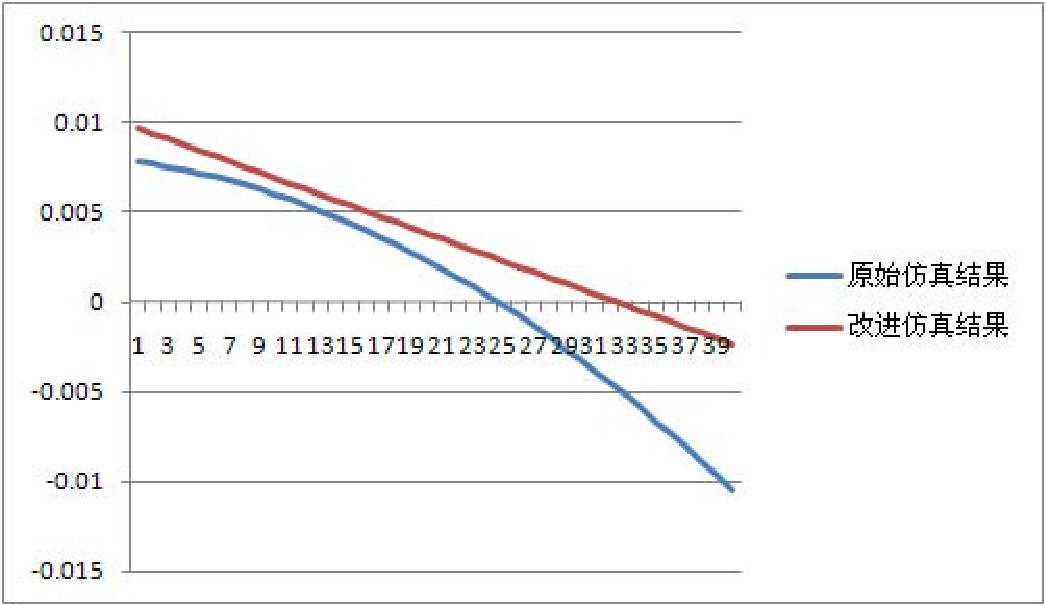
\includegraphics{improve9.pdf}}
 % GNUPLOT: LaTeX picture
\setlength{\unitlength}{0.240900pt}
\ifx\plotpoint\undefined\newsavebox{\plotpoint}\fi
\begin{picture}(1500,900)(0,0)
\sbox{\plotpoint}{\rule[-0.200pt]{0.400pt}{0.400pt}}%
\put(211.0,82.0){\rule[-0.200pt]{4.818pt}{0.400pt}}
\put(191,82){\makebox(0,0)[r]{-0.02}}
\put(1419.0,82.0){\rule[-0.200pt]{4.818pt}{0.400pt}}
\put(211.0,143.0){\rule[-0.200pt]{4.818pt}{0.400pt}}
\put(191,143){\makebox(0,0)[r]{-0.015}}
\put(1419.0,143.0){\rule[-0.200pt]{4.818pt}{0.400pt}}
\put(211.0,203.0){\rule[-0.200pt]{4.818pt}{0.400pt}}
\put(191,203){\makebox(0,0)[r]{-0.01}}
\put(1419.0,203.0){\rule[-0.200pt]{4.818pt}{0.400pt}}
\put(211.0,264.0){\rule[-0.200pt]{4.818pt}{0.400pt}}
\put(191,264){\makebox(0,0)[r]{-0.005}}
\put(1419.0,264.0){\rule[-0.200pt]{4.818pt}{0.400pt}}
\put(211.0,325.0){\rule[-0.200pt]{4.818pt}{0.400pt}}
\put(191,325){\makebox(0,0)[r]{ 0}}
\put(1419.0,325.0){\rule[-0.200pt]{4.818pt}{0.400pt}}
\put(211.0,386.0){\rule[-0.200pt]{4.818pt}{0.400pt}}
\put(191,386){\makebox(0,0)[r]{ 0.005}}
\put(1419.0,386.0){\rule[-0.200pt]{4.818pt}{0.400pt}}
\put(211.0,446.0){\rule[-0.200pt]{4.818pt}{0.400pt}}
\put(191,446){\makebox(0,0)[r]{ 0.01}}
\put(1419.0,446.0){\rule[-0.200pt]{4.818pt}{0.400pt}}
\put(211.0,507.0){\rule[-0.200pt]{4.818pt}{0.400pt}}
\put(191,507){\makebox(0,0)[r]{ 0.015}}
\put(1419.0,507.0){\rule[-0.200pt]{4.818pt}{0.400pt}}
\put(211.0,568.0){\rule[-0.200pt]{4.818pt}{0.400pt}}
\put(191,568){\makebox(0,0)[r]{ 0.02}}
\put(1419.0,568.0){\rule[-0.200pt]{4.818pt}{0.400pt}}
\put(211.0,628.0){\rule[-0.200pt]{4.818pt}{0.400pt}}
\put(191,628){\makebox(0,0)[r]{ 0.025}}
\put(1419.0,628.0){\rule[-0.200pt]{4.818pt}{0.400pt}}
\put(211.0,689.0){\rule[-0.200pt]{4.818pt}{0.400pt}}
\put(191,689){\makebox(0,0)[r]{ 0.03}}
\put(1419.0,689.0){\rule[-0.200pt]{4.818pt}{0.400pt}}
\put(211.0,82.0){\rule[-0.200pt]{0.400pt}{4.818pt}}
\put(211,41){\makebox(0,0){ 1}}
\put(211.0,839.0){\rule[-0.200pt]{0.400pt}{4.818pt}}
\put(274.0,82.0){\rule[-0.200pt]{0.400pt}{4.818pt}}
\put(274,41){\makebox(0,0){ 3}}
\put(274.0,839.0){\rule[-0.200pt]{0.400pt}{4.818pt}}
\put(337.0,82.0){\rule[-0.200pt]{0.400pt}{4.818pt}}
\put(337,41){\makebox(0,0){ 5}}
\put(337.0,839.0){\rule[-0.200pt]{0.400pt}{4.818pt}}
\put(400.0,82.0){\rule[-0.200pt]{0.400pt}{4.818pt}}
\put(400,41){\makebox(0,0){ 7}}
\put(400.0,839.0){\rule[-0.200pt]{0.400pt}{4.818pt}}
\put(463.0,82.0){\rule[-0.200pt]{0.400pt}{4.818pt}}
\put(463,41){\makebox(0,0){ 9}}
\put(463.0,839.0){\rule[-0.200pt]{0.400pt}{4.818pt}}
\put(526.0,82.0){\rule[-0.200pt]{0.400pt}{4.818pt}}
\put(526,41){\makebox(0,0){ 11}}
\put(526.0,839.0){\rule[-0.200pt]{0.400pt}{4.818pt}}
\put(589.0,82.0){\rule[-0.200pt]{0.400pt}{4.818pt}}
\put(589,41){\makebox(0,0){ 13}}
\put(589.0,839.0){\rule[-0.200pt]{0.400pt}{4.818pt}}
\put(652.0,82.0){\rule[-0.200pt]{0.400pt}{4.818pt}}
\put(652,41){\makebox(0,0){ 15}}
\put(652.0,839.0){\rule[-0.200pt]{0.400pt}{4.818pt}}
\put(715.0,82.0){\rule[-0.200pt]{0.400pt}{4.818pt}}
\put(715,41){\makebox(0,0){ 17}}
\put(715.0,839.0){\rule[-0.200pt]{0.400pt}{4.818pt}}
\put(778.0,82.0){\rule[-0.200pt]{0.400pt}{4.818pt}}
\put(778,41){\makebox(0,0){ 19}}
\put(778.0,839.0){\rule[-0.200pt]{0.400pt}{4.818pt}}
\put(841.0,82.0){\rule[-0.200pt]{0.400pt}{4.818pt}}
\put(841,41){\makebox(0,0){ 21}}
\put(841.0,839.0){\rule[-0.200pt]{0.400pt}{4.818pt}}
\put(904.0,82.0){\rule[-0.200pt]{0.400pt}{4.818pt}}
\put(904,41){\makebox(0,0){ 23}}
\put(904.0,839.0){\rule[-0.200pt]{0.400pt}{4.818pt}}
\put(967.0,82.0){\rule[-0.200pt]{0.400pt}{4.818pt}}
\put(967,41){\makebox(0,0){ 25}}
\put(967.0,839.0){\rule[-0.200pt]{0.400pt}{4.818pt}}
\put(1030.0,82.0){\rule[-0.200pt]{0.400pt}{4.818pt}}
\put(1030,41){\makebox(0,0){ 27}}
\put(1030.0,839.0){\rule[-0.200pt]{0.400pt}{4.818pt}}
\put(1093.0,82.0){\rule[-0.200pt]{0.400pt}{4.818pt}}
\put(1093,41){\makebox(0,0){ 29}}
\put(1093.0,839.0){\rule[-0.200pt]{0.400pt}{4.818pt}}
\put(1156.0,82.0){\rule[-0.200pt]{0.400pt}{4.818pt}}
\put(1156,41){\makebox(0,0){ 31}}
\put(1156.0,839.0){\rule[-0.200pt]{0.400pt}{4.818pt}}
\put(1219.0,82.0){\rule[-0.200pt]{0.400pt}{4.818pt}}
\put(1219,41){\makebox(0,0){ 33}}
\put(1219.0,839.0){\rule[-0.200pt]{0.400pt}{4.818pt}}
\put(1282.0,82.0){\rule[-0.200pt]{0.400pt}{4.818pt}}
\put(1282,41){\makebox(0,0){ 35}}
\put(1282.0,839.0){\rule[-0.200pt]{0.400pt}{4.818pt}}
\put(1345.0,82.0){\rule[-0.200pt]{0.400pt}{4.818pt}}
\put(1345,41){\makebox(0,0){ 37}}
\put(1345.0,839.0){\rule[-0.200pt]{0.400pt}{4.818pt}}
\put(1408.0,82.0){\rule[-0.200pt]{0.400pt}{4.818pt}}
\put(1408,41){\makebox(0,0){ 39}}
\put(1408.0,839.0){\rule[-0.200pt]{0.400pt}{4.818pt}}
\put(211.0,82.0){\rule[-0.200pt]{0.400pt}{187.179pt}}
\put(211.0,82.0){\rule[-0.200pt]{295.825pt}{0.400pt}}
\put(1439.0,82.0){\rule[-0.200pt]{0.400pt}{187.179pt}}
\put(211.0,859.0){\rule[-0.200pt]{295.825pt}{0.400pt}}
\put(30,470){\makebox(0,0){\rotatebox{90}{用户贡献}}}
\put(1279,819){\makebox(0,0)[r]{仿真数据}}
\put(1299.0,819.0){\rule[-0.200pt]{24.090pt}{0.400pt}}
\put(211,423){\usebox{\plotpoint}}
\put(211,421.17){\rule{6.300pt}{0.400pt}}
\multiput(211.00,422.17)(17.924,-2.000){2}{\rule{3.150pt}{0.400pt}}
\multiput(242.00,419.94)(4.575,-0.468){5}{\rule{3.300pt}{0.113pt}}
\multiput(242.00,420.17)(25.151,-4.000){2}{\rule{1.650pt}{0.400pt}}
\multiput(305.00,415.94)(4.575,-0.468){5}{\rule{3.300pt}{0.113pt}}
\multiput(305.00,416.17)(25.151,-4.000){2}{\rule{1.650pt}{0.400pt}}
\multiput(337.00,413.60)(4.429,0.468){5}{\rule{3.200pt}{0.113pt}}
\multiput(337.00,412.17)(24.358,4.000){2}{\rule{1.600pt}{0.400pt}}
\put(274.0,417.0){\rule[-0.200pt]{7.468pt}{0.400pt}}
\multiput(400.00,415.93)(2.013,-0.488){13}{\rule{1.650pt}{0.117pt}}
\multiput(400.00,416.17)(27.575,-8.000){2}{\rule{0.825pt}{0.400pt}}
\multiput(431.00,407.94)(4.575,-0.468){5}{\rule{3.300pt}{0.113pt}}
\multiput(431.00,408.17)(25.151,-4.000){2}{\rule{1.650pt}{0.400pt}}
\multiput(463.00,403.93)(3.382,-0.477){7}{\rule{2.580pt}{0.115pt}}
\multiput(463.00,404.17)(25.645,-5.000){2}{\rule{1.290pt}{0.400pt}}
\multiput(494.00,400.59)(3.493,0.477){7}{\rule{2.660pt}{0.115pt}}
\multiput(494.00,399.17)(26.479,5.000){2}{\rule{1.330pt}{0.400pt}}
\multiput(526.00,403.93)(3.382,-0.477){7}{\rule{2.580pt}{0.115pt}}
\multiput(526.00,404.17)(25.645,-5.000){2}{\rule{1.290pt}{0.400pt}}
\multiput(557.00,398.93)(2.079,-0.488){13}{\rule{1.700pt}{0.117pt}}
\multiput(557.00,399.17)(28.472,-8.000){2}{\rule{0.850pt}{0.400pt}}
\multiput(589.00,390.93)(3.382,-0.477){7}{\rule{2.580pt}{0.115pt}}
\multiput(589.00,391.17)(25.645,-5.000){2}{\rule{1.290pt}{0.400pt}}
\multiput(620.00,385.94)(4.575,-0.468){5}{\rule{3.300pt}{0.113pt}}
\multiput(620.00,386.17)(25.151,-4.000){2}{\rule{1.650pt}{0.400pt}}
\multiput(652.00,381.93)(2.013,-0.488){13}{\rule{1.650pt}{0.117pt}}
\multiput(652.00,382.17)(27.575,-8.000){2}{\rule{0.825pt}{0.400pt}}
\multiput(683.00,373.95)(6.937,-0.447){3}{\rule{4.367pt}{0.108pt}}
\multiput(683.00,374.17)(22.937,-3.000){2}{\rule{2.183pt}{0.400pt}}
\multiput(715.00,370.93)(3.382,-0.477){7}{\rule{2.580pt}{0.115pt}}
\multiput(715.00,371.17)(25.645,-5.000){2}{\rule{1.290pt}{0.400pt}}
\multiput(746.00,365.93)(1.834,-0.489){15}{\rule{1.522pt}{0.118pt}}
\multiput(746.00,366.17)(28.841,-9.000){2}{\rule{0.761pt}{0.400pt}}
\multiput(778.00,358.60)(4.429,0.468){5}{\rule{3.200pt}{0.113pt}}
\multiput(778.00,357.17)(24.358,4.000){2}{\rule{1.600pt}{0.400pt}}
\multiput(809.00,360.92)(1.250,-0.493){23}{\rule{1.085pt}{0.119pt}}
\multiput(809.00,361.17)(29.749,-13.000){2}{\rule{0.542pt}{0.400pt}}
\multiput(841.00,349.60)(4.429,0.468){5}{\rule{3.200pt}{0.113pt}}
\multiput(841.00,348.17)(24.358,4.000){2}{\rule{1.600pt}{0.400pt}}
\multiput(872.00,351.92)(1.009,-0.494){29}{\rule{0.900pt}{0.119pt}}
\multiput(872.00,352.17)(30.132,-16.000){2}{\rule{0.450pt}{0.400pt}}
\put(904,335.67){\rule{7.468pt}{0.400pt}}
\multiput(904.00,336.17)(15.500,-1.000){2}{\rule{3.734pt}{0.400pt}}
\multiput(935.00,334.93)(2.841,-0.482){9}{\rule{2.233pt}{0.116pt}}
\multiput(935.00,335.17)(27.365,-6.000){2}{\rule{1.117pt}{0.400pt}}
\multiput(967.00,328.92)(1.590,-0.491){17}{\rule{1.340pt}{0.118pt}}
\multiput(967.00,329.17)(28.219,-10.000){2}{\rule{0.670pt}{0.400pt}}
\put(998,318.17){\rule{6.500pt}{0.400pt}}
\multiput(998.00,319.17)(18.509,-2.000){2}{\rule{3.250pt}{0.400pt}}
\multiput(1030.00,316.92)(0.977,-0.494){29}{\rule{0.875pt}{0.119pt}}
\multiput(1030.00,317.17)(29.184,-16.000){2}{\rule{0.438pt}{0.400pt}}
\multiput(1061.00,300.93)(2.079,-0.488){13}{\rule{1.700pt}{0.117pt}}
\multiput(1061.00,301.17)(28.472,-8.000){2}{\rule{0.850pt}{0.400pt}}
\multiput(1093.00,292.93)(2.013,-0.488){13}{\rule{1.650pt}{0.117pt}}
\multiput(1093.00,293.17)(27.575,-8.000){2}{\rule{0.825pt}{0.400pt}}
\put(1124,284.67){\rule{7.709pt}{0.400pt}}
\multiput(1124.00,285.17)(16.000,-1.000){2}{\rule{3.854pt}{0.400pt}}
\multiput(1156.00,283.92)(1.590,-0.491){17}{\rule{1.340pt}{0.118pt}}
\multiput(1156.00,284.17)(28.219,-10.000){2}{\rule{0.670pt}{0.400pt}}
\multiput(1187.00,273.92)(1.642,-0.491){17}{\rule{1.380pt}{0.118pt}}
\multiput(1187.00,274.17)(29.136,-10.000){2}{\rule{0.690pt}{0.400pt}}
\multiput(1219.00,263.95)(6.714,-0.447){3}{\rule{4.233pt}{0.108pt}}
\multiput(1219.00,264.17)(22.214,-3.000){2}{\rule{2.117pt}{0.400pt}}
\multiput(1250.00,260.92)(1.642,-0.491){17}{\rule{1.380pt}{0.118pt}}
\multiput(1250.00,261.17)(29.136,-10.000){2}{\rule{0.690pt}{0.400pt}}
\multiput(1282.00,250.92)(1.439,-0.492){19}{\rule{1.227pt}{0.118pt}}
\multiput(1282.00,251.17)(28.453,-11.000){2}{\rule{0.614pt}{0.400pt}}
\multiput(1313.00,239.92)(1.642,-0.491){17}{\rule{1.380pt}{0.118pt}}
\multiput(1313.00,240.17)(29.136,-10.000){2}{\rule{0.690pt}{0.400pt}}
\multiput(1345.00,229.93)(2.013,-0.488){13}{\rule{1.650pt}{0.117pt}}
\multiput(1345.00,230.17)(27.575,-8.000){2}{\rule{0.825pt}{0.400pt}}
\multiput(1376.00,221.93)(3.493,-0.477){7}{\rule{2.660pt}{0.115pt}}
\multiput(1376.00,222.17)(26.479,-5.000){2}{\rule{1.330pt}{0.400pt}}
\multiput(1408.00,216.92)(1.315,-0.492){21}{\rule{1.133pt}{0.119pt}}
\multiput(1408.00,217.17)(28.648,-12.000){2}{\rule{0.567pt}{0.400pt}}
\put(368.0,417.0){\rule[-0.200pt]{7.709pt}{0.400pt}}
\put(1279,768){\makebox(0,0)[r]{改进数据}}
\put(1299.0,768.0){\rule[-0.200pt]{24.090pt}{0.400pt}}
\put(211,526){\usebox{\plotpoint}}
\multiput(211.58,523.28)(0.497,-0.695){59}{\rule{0.120pt}{0.655pt}}
\multiput(210.17,524.64)(31.000,-41.641){2}{\rule{0.400pt}{0.327pt}}
\multiput(242.00,481.92)(0.697,-0.496){43}{\rule{0.657pt}{0.120pt}}
\multiput(242.00,482.17)(30.637,-23.000){2}{\rule{0.328pt}{0.400pt}}
\multiput(274.00,458.92)(0.919,-0.495){31}{\rule{0.829pt}{0.119pt}}
\multiput(274.00,459.17)(29.279,-17.000){2}{\rule{0.415pt}{0.400pt}}
\multiput(305.00,441.92)(1.486,-0.492){19}{\rule{1.264pt}{0.118pt}}
\multiput(305.00,442.17)(29.377,-11.000){2}{\rule{0.632pt}{0.400pt}}
\multiput(337.00,430.93)(1.776,-0.489){15}{\rule{1.478pt}{0.118pt}}
\multiput(337.00,431.17)(27.933,-9.000){2}{\rule{0.739pt}{0.400pt}}
\multiput(368.00,421.92)(0.847,-0.495){35}{\rule{0.774pt}{0.119pt}}
\multiput(368.00,422.17)(30.394,-19.000){2}{\rule{0.387pt}{0.400pt}}
\multiput(431.00,402.92)(1.158,-0.494){25}{\rule{1.014pt}{0.119pt}}
\multiput(431.00,403.17)(29.895,-14.000){2}{\rule{0.507pt}{0.400pt}}
\multiput(463.00,388.95)(6.714,-0.447){3}{\rule{4.233pt}{0.108pt}}
\multiput(463.00,389.17)(22.214,-3.000){2}{\rule{2.117pt}{0.400pt}}
\put(494,386.67){\rule{7.709pt}{0.400pt}}
\multiput(494.00,386.17)(16.000,1.000){2}{\rule{3.854pt}{0.400pt}}
\multiput(526.00,386.93)(1.776,-0.489){15}{\rule{1.478pt}{0.118pt}}
\multiput(526.00,387.17)(27.933,-9.000){2}{\rule{0.739pt}{0.400pt}}
\multiput(557.00,377.93)(2.079,-0.488){13}{\rule{1.700pt}{0.117pt}}
\multiput(557.00,378.17)(28.472,-8.000){2}{\rule{0.850pt}{0.400pt}}
\multiput(589.00,369.93)(3.382,-0.477){7}{\rule{2.580pt}{0.115pt}}
\multiput(589.00,370.17)(25.645,-5.000){2}{\rule{1.290pt}{0.400pt}}
\put(400.0,404.0){\rule[-0.200pt]{7.468pt}{0.400pt}}
\multiput(652.00,366.61)(6.714,0.447){3}{\rule{4.233pt}{0.108pt}}
\multiput(652.00,365.17)(22.214,3.000){2}{\rule{2.117pt}{0.400pt}}
\multiput(683.00,367.93)(1.834,-0.489){15}{\rule{1.522pt}{0.118pt}}
\multiput(683.00,368.17)(28.841,-9.000){2}{\rule{0.761pt}{0.400pt}}
\multiput(715.00,358.93)(3.382,-0.477){7}{\rule{2.580pt}{0.115pt}}
\multiput(715.00,359.17)(25.645,-5.000){2}{\rule{1.290pt}{0.400pt}}
\put(746,353.67){\rule{7.709pt}{0.400pt}}
\multiput(746.00,354.17)(16.000,-1.000){2}{\rule{3.854pt}{0.400pt}}
\multiput(778.00,352.93)(3.382,-0.477){7}{\rule{2.580pt}{0.115pt}}
\multiput(778.00,353.17)(25.645,-5.000){2}{\rule{1.290pt}{0.400pt}}
\put(809,348.67){\rule{7.709pt}{0.400pt}}
\multiput(809.00,348.17)(16.000,1.000){2}{\rule{3.854pt}{0.400pt}}
\multiput(841.00,350.60)(4.429,0.468){5}{\rule{3.200pt}{0.113pt}}
\multiput(841.00,349.17)(24.358,4.000){2}{\rule{1.600pt}{0.400pt}}
\multiput(872.00,352.92)(1.642,-0.491){17}{\rule{1.380pt}{0.118pt}}
\multiput(872.00,353.17)(29.136,-10.000){2}{\rule{0.690pt}{0.400pt}}
\multiput(904.00,344.59)(2.751,0.482){9}{\rule{2.167pt}{0.116pt}}
\multiput(904.00,343.17)(26.503,6.000){2}{\rule{1.083pt}{0.400pt}}
\multiput(935.00,348.93)(3.493,-0.477){7}{\rule{2.660pt}{0.115pt}}
\multiput(935.00,349.17)(26.479,-5.000){2}{\rule{1.330pt}{0.400pt}}
\multiput(967.00,343.94)(4.429,-0.468){5}{\rule{3.200pt}{0.113pt}}
\multiput(967.00,344.17)(24.358,-4.000){2}{\rule{1.600pt}{0.400pt}}
\multiput(998.00,341.60)(4.575,0.468){5}{\rule{3.300pt}{0.113pt}}
\multiput(998.00,340.17)(25.151,4.000){2}{\rule{1.650pt}{0.400pt}}
\multiput(1030.00,343.93)(2.751,-0.482){9}{\rule{2.167pt}{0.116pt}}
\multiput(1030.00,344.17)(26.503,-6.000){2}{\rule{1.083pt}{0.400pt}}
\multiput(1061.00,339.60)(4.575,0.468){5}{\rule{3.300pt}{0.113pt}}
\multiput(1061.00,338.17)(25.151,4.000){2}{\rule{1.650pt}{0.400pt}}
\multiput(1093.00,341.93)(2.323,-0.485){11}{\rule{1.871pt}{0.117pt}}
\multiput(1093.00,342.17)(27.116,-7.000){2}{\rule{0.936pt}{0.400pt}}
\multiput(1124.00,336.59)(3.493,0.477){7}{\rule{2.660pt}{0.115pt}}
\multiput(1124.00,335.17)(26.479,5.000){2}{\rule{1.330pt}{0.400pt}}
\multiput(1156.00,339.95)(6.714,-0.447){3}{\rule{4.233pt}{0.108pt}}
\multiput(1156.00,340.17)(22.214,-3.000){2}{\rule{2.117pt}{0.400pt}}
\put(1187,336.17){\rule{6.500pt}{0.400pt}}
\multiput(1187.00,337.17)(18.509,-2.000){2}{\rule{3.250pt}{0.400pt}}
\multiput(1219.00,336.59)(3.382,0.477){7}{\rule{2.580pt}{0.115pt}}
\multiput(1219.00,335.17)(25.645,5.000){2}{\rule{1.290pt}{0.400pt}}
\put(1250,339.17){\rule{6.500pt}{0.400pt}}
\multiput(1250.00,340.17)(18.509,-2.000){2}{\rule{3.250pt}{0.400pt}}
\multiput(1282.00,337.95)(6.714,-0.447){3}{\rule{4.233pt}{0.108pt}}
\multiput(1282.00,338.17)(22.214,-3.000){2}{\rule{2.117pt}{0.400pt}}
\put(1313,335.67){\rule{7.709pt}{0.400pt}}
\multiput(1313.00,335.17)(16.000,1.000){2}{\rule{3.854pt}{0.400pt}}
\put(1345,335.17){\rule{6.300pt}{0.400pt}}
\multiput(1345.00,336.17)(17.924,-2.000){2}{\rule{3.150pt}{0.400pt}}
\multiput(1376.00,333.94)(4.575,-0.468){5}{\rule{3.300pt}{0.113pt}}
\multiput(1376.00,334.17)(25.151,-4.000){2}{\rule{1.650pt}{0.400pt}}
\put(1408,329.67){\rule{7.468pt}{0.400pt}}
\multiput(1408.00,330.17)(15.500,-1.000){2}{\rule{3.734pt}{0.400pt}}
\put(211,526){\makebox(0,0){$+$}}
\put(242,483){\makebox(0,0){$+$}}
\put(274,460){\makebox(0,0){$+$}}
\put(305,443){\makebox(0,0){$+$}}
\put(337,432){\makebox(0,0){$+$}}
\put(368,423){\makebox(0,0){$+$}}
\put(400,404){\makebox(0,0){$+$}}
\put(431,404){\makebox(0,0){$+$}}
\put(463,390){\makebox(0,0){$+$}}
\put(494,387){\makebox(0,0){$+$}}
\put(526,388){\makebox(0,0){$+$}}
\put(557,379){\makebox(0,0){$+$}}
\put(589,371){\makebox(0,0){$+$}}
\put(620,366){\makebox(0,0){$+$}}
\put(652,366){\makebox(0,0){$+$}}
\put(683,369){\makebox(0,0){$+$}}
\put(715,360){\makebox(0,0){$+$}}
\put(746,355){\makebox(0,0){$+$}}
\put(778,354){\makebox(0,0){$+$}}
\put(809,349){\makebox(0,0){$+$}}
\put(841,350){\makebox(0,0){$+$}}
\put(872,354){\makebox(0,0){$+$}}
\put(904,344){\makebox(0,0){$+$}}
\put(935,350){\makebox(0,0){$+$}}
\put(967,345){\makebox(0,0){$+$}}
\put(998,341){\makebox(0,0){$+$}}
\put(1030,345){\makebox(0,0){$+$}}
\put(1061,339){\makebox(0,0){$+$}}
\put(1093,343){\makebox(0,0){$+$}}
\put(1124,336){\makebox(0,0){$+$}}
\put(1156,341){\makebox(0,0){$+$}}
\put(1187,338){\makebox(0,0){$+$}}
\put(1219,336){\makebox(0,0){$+$}}
\put(1250,341){\makebox(0,0){$+$}}
\put(1282,339){\makebox(0,0){$+$}}
\put(1313,336){\makebox(0,0){$+$}}
\put(1345,337){\makebox(0,0){$+$}}
\put(1376,335){\makebox(0,0){$+$}}
\put(1408,331){\makebox(0,0){$+$}}
\put(1439,330){\makebox(0,0){$+$}}
\put(1349,768){\makebox(0,0){$+$}}
\put(620.0,366.0){\rule[-0.200pt]{7.709pt}{0.400pt}}
\put(211.0,82.0){\rule[-0.200pt]{0.400pt}{187.179pt}}
\put(211.0,82.0){\rule[-0.200pt]{295.825pt}{0.400pt}}
\put(1439.0,82.0){\rule[-0.200pt]{0.400pt}{187.179pt}}
\put(211.0,859.0){\rule[-0.200pt]{295.825pt}{0.400pt}}
\end{picture}
 
 \caption{\small{\textbf{提升边缘用户动机的仿真结果}}}
  \label{fig:improve9}
\end{figure}

边缘用户是整个社区中参与动机最弱,参与程度最低的群体。运用各种手段提升
其参与动机,使其转变为其它类型的用户是社区的重要任务之一。社区可以采取
的措施包括鼓励用户多参与协同活动,可以设置一些实验性作品供用户练习、熟
悉,同时还不必考虑是否会得到负面反馈。准备各种示范材料、帮助手册用以提
升用户的编辑水平,帮助他们尽快适应协同编辑的模式。在宽松的环境下,边缘
用户容易培养自信,提升参与动机,同时提升编辑的质量。尽管绝大部分边缘用户在
其整个社区生涯中都不会改变其行为特点,但是社区仍然应该注重对边缘用户的关注。
社区只有拥有数量庞大的边缘用户才能不断涌现出高质量的用户。

\section{本章小结}

动机因素模型的建立为分析维基百科社区中的用户动机提供了有力的工具。仿真
的结果表明,动机模型能够较好地反应用户参与知识协同的动机。利用
系统动力学模型,不但揭示了不同动机因素对于用户行为的影响,还反映了行为
结果对于动机水平的影响,使得动机与行为间的关系形成了完整的闭环。在此基础上,进
一步针对不同类型用户的特点提出管理建议,并利用仿真模型验证改进的有效性。
社区建设者可以根据这些结果有针对性地做出改进,从而促进社区更好地发展。



%%% Local Variables: 
%%% mode: latex
%%% TeX-master: t
%%% End: 

\bibliographystyle{unabuser}
\bibliography{../../bibtex/elsevier,../../bibtex/emerald,../../bibtex/chinese,../../bibtex/jstor,../../bibtex/citeseer,../../bibtex/acm,../../bibtex/wiley,../../bibtex/book,../../bibtex/thesis,../../bibtex/ebsco,../../bibtex/old,../../bibtex/ieee,../../bibtex/internet,../../bibtex/ssrn,../../bibtex/apa,../../bibtex/blackwell,../../bibtex/sage,../../bibtex/springer,../../bibtex/MESharp,../../bibtex/taylor}

\end{document}

%%% Local Variables: 
%%% mode: latex
%%% TeX-master: t
%%% End: 
